% version of 03-19-18
\documentclass[envcountchap]{svmono}
%\usepackage{amsfonts,amsmath,amsthm,amssymb,fullpage,makeidx,epsfig}

\usepackage{mathptmx}
\usepackage{amssymb}
\usepackage{helvet}
\usepackage{courier}
\usepackage{makeidx}
\usepackage{graphicx}
\usepackage{multicol}
\usepackage{epsfig}
\usepackage[bottom]{footmisc}% places footnotes at page bottom

\setcounter{tocdepth}{5}

%\newtheorem{note}{Note}
\newtheorem{corol}{Corollary}[chapter]
\newtheorem{prop}{Proposition}[chapter]
%\newtheorem{lem}{Lemma}[chapter]
%\newtheorem{thm}{Theorem}[chapter]

\makeindex

\begin{document}


\input preamble

\author{Arnold L.~Rosenberg \and Denis Trystram}
\title{Understand Mathematics, Understand Computing}
\subtitle{Discrete Mathematics that All Computing Students Should Know}

\maketitle

\begin{center}
{\Large\bf Understand Mathematics, Understand Computing} \\
{\large\it Discrete Mathematics that All Computing Students Should Know}
\end{center}


\begin{center}
\begin{tabular}{ccc}
{\large Arnold L.~Rosenberg} & & {\large Denis Trystram} \\
Distinguished University Professor Emeritus
  & & Distinguished Professor \\
University of Massachusetts  & & University of Grenoble \\
Amherst, MA 01003, USA       & & Grenoble, FRANCE \\
{\small\tt rsnbrg@cs.umass.edu} & & {\small\tt denis.trystram@imag.fr}
\end{tabular}
\end{center}

\vspace*{.25in}

{\it Mathematics is the foundation on which the edifice of Computing
  stands}

\begin{figure}[h]
\centerline{\epsfig{figure=MATH.eps,height=5truein}}
\end{figure}



%{\small
%\copyright 2006,2007,2008,2009 Arnold L.~Rosenberg} \\
%{\small All rights reserved}
%\end{center}


\frontmatter

%%version of 05-01-20
%%%%%%%%%%%%%%%%%%%%%%% dedic.tex %%%%%%%%%%%%%%%%%%%%%%%%%%%%%%%%%
%
% sample dedication
%
% Use this file as a template for your own input.
%
%%%%%%%%%%%%%%%%%%%%%%%% Springer %%%%%%%%%%%%%%%%%%%%%%%%%%

\begin{dedication}
To my beloved wife, Susan, for her infinite patience during my extended episodes of ``cerebral absence.''

\smallskip

\noindent
To Professor Oscar Zariski, who changed my life by introducing me to ``real" mathematics.
\smallskip

\noindent
With love to my wife C\'ecile and my children Alice and No\'e who help me to stay connected to the ``real'' world. 
\bigskip

\noindent To all past students who inspired this book.

\noindent To all future students who will read this book.
\end{dedication}

\vspace*{.25in}

\centerline{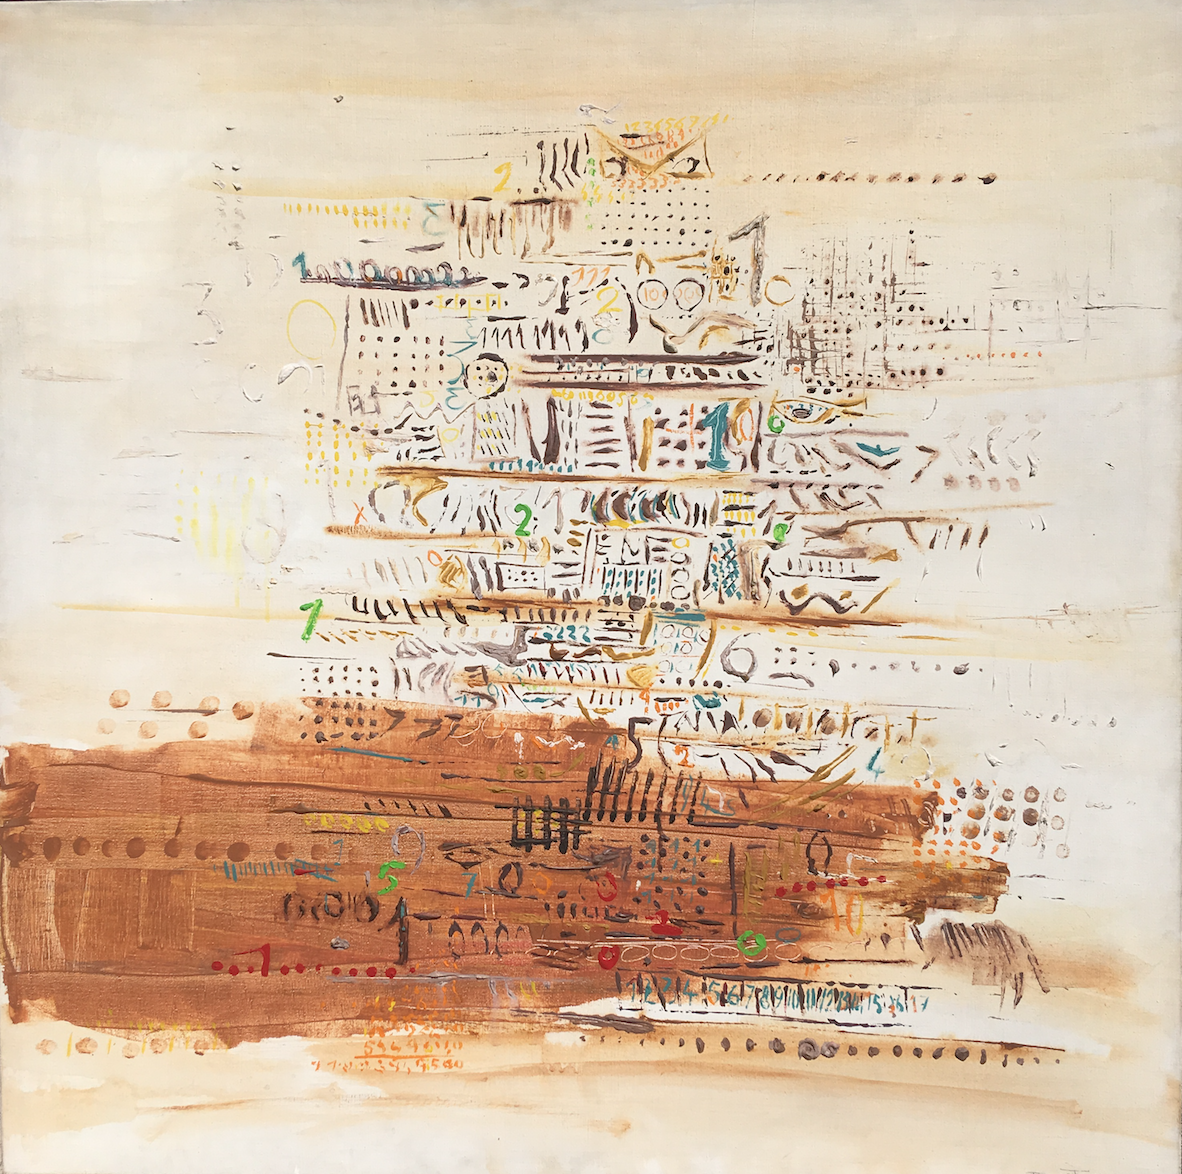
\includegraphics[scale=0.75]{AdditionForSpringer.png}}

\medskip

\centerline{{\large\em  Addition} \hspace*{4.5in} {\small Roger Trystram, 1973}}



%*********REVISED 01-31-08

%\addcontentsline{toc}{chapter}{Capsule Biography of the Author}
%\input{capsulebio}
%*********REVISED 07-02-08

\tableofcontents

%\addcontentsline{toc}{chapter}{Preface and Manifesto}
%%version of 04-09-19 

\chapter*{PREFACE AND MANIFESTO}


\begin{center}
{\it Entia non sunt multiplicanda praeter necessitatem.} \\
\hspace*{3in}{\footnotesize {\bf Occam's Razor}}
\end{center}

\noindent
This famous admonition by William of Occam (14th cent.) to strive for
simplicity is worth heeding when seeking mathematical models of
computational phenomena.

\section{The ``Manifesto'' Underlying This Text}
\label{sec:Manifesto}

**ADD SHORT PARAGRAPH FOR EACH POINT

\begin{itemize}
\item
We aim for UNDERSTANDING rather than just knowledge
\item
We want to help students/readers THINK rather than just learn —
which explains multiple proofs
\item
We want to expose the reader to some culture (as an aid to thinking
and understanding) — which explains some digressions and stories
\item
Part of the culture comes via the $\oplus$ sections … even if they are
rather short and informal.
\end{itemize}




As the technology that enabled both the hardware and software systems
of modern computers has advanced, the ability to design and utilize
such systems ``by the seat of one's pants'' has commensurately
decreased.  A vast array of formal aids for the activities of
designing, analyzing, utilizing, and verifying computer systemshas
developed, and mathematical tools have always been at or near the
forefront of such aids.

The fundamental goal of this book---and, therefore, of each of its
chapters and sections---is to endow the reader with an operational
level of conceptual and methodological understanding of the discrete
mathematics that is used to study and understand the activity of
computing and the systems that enable that activity.  We construe an
``operational'' level of understanding to be one that enables the
reader to ``do'' the relevant mathematics.

Somewhat surprising to the non-mathematician, a large portion of
``doing'' mathematics, the often-touted ``queen of the sciences'', is
pattern-matching---albeit of a monumentally sophisticated variety.
Mathematicians are trained to understand pieces of reality to a depth
that allows them to understand how apparently unrelated concepts $A$
and $B$ can be conceptualized via the same abstract representation,
and to analyze (computational, in our bailiwick) advantages to
exploiting such representations.

Toward the end of guiding the reader through this forest of
abstractions, we categorize our targets in three ways
\begin{enumerate}
\item
{\it Fundamental concepts}

{\sf Examples:}
\begin{itemize}
\item
sets---and their embellishments: tuples, arrays, tables, etc.---as the
embodiment of {\it object}
\item
numbers---and their operational manifestations, numerals---as the
embodiment of {\it quantity}
\item
graphs---in their many, varied, forms---as the embodiment of {\it
  connectivity} and {\it relationship}
\item
algebras---adding operations to sets, numbers, and graphs---as the
embodiment of {\it structured dynamism} and {\it computing}
\end{itemize}

\item
{\it Fundamental representations}

{\sf Examples:}
\begin{itemize}
\item
viewing numbers via the metaphors of: slices of pie, tokens arranged in
stylized ways, rectangles of varying dimensions
\item
using grouping and/or replication to represent relationships among
objects
\item
viewing interrelated objects via varying structures: tables, tuples,
graphs, geometric drawing
\end{itemize}

\item
{\it Fundamental tools/techniques}

{\sf Examples:}
\begin{itemize}
\item
using induction to expand from simple examples to complex ones
\item
using integration to approximate summation, and vice versa, to
(mentally) ``hop'' between the discrete and continuous worlds
\item
using the conceptual tools of asymptotics to argue qualitatively about
quantitative phenomena.
\end{itemize}
\end{enumerate}

%chapter
%*********REVISED 02-04-08


%\addcontentsline{toc}{chapter}{List of Acronyms}
%\input{acronym}


\mainmatter

%%%%%%%%%%%%%%%%%%%%%%%%%%%%%

%version of 06-18-19

\chapter{INTRODUCTION}
\label{ch:intro}

\begin{quote}
{\em I have only made this letter longer because I have not had the
  time to make it shorter.}  \\
\hspace*{1.5in}Blaise Pascal, {\it The Provincial Letters}
(Letter 16, 1657)
\end{quote}


\section{Why Is This Book {\em Needed?}}
\label{sec:bookneeded}

How much mathematics does an aspiring computing professional
need---and at what level of expertise?  We believe that the answer to
this pedagogically fundamental question is time dependent.

\medskip

\noindent {\it The early generation}.
In the early days of computing, all aspects of the field were
considered the domain of the ``techies''---the engineers and
scientists and mathematicians who designed the early computers and
figured out how to use them to solve a range of (mostly
compute-intensive) problems.  Back then, one expected every computing
professional to have a mastery of many mathematical topics.

\medskip

\noindent {\it Children of the early generation}.
Times---and the field of computing---changed.  The ``techies'' were
able to craft a variety of sophisticated tools that opened up the
world of computing to the general population.  Even people at the
lower levels of the educational edifice were able to use imagination
and ingenuity, rather than theorems and formulas, to produce
impressive software artifacts of considerable utility.

\medskip

\noindent {\it The modern generation}.
Pendulums were made to swing.  As we note in our {\it Manifesto}, we
now encounter almost daily problems that arise from unanticipated
concomitants of the often unstructured ingenuity that produced various
software artifacts.  Many would say that we need a renewed commitment
to technical discipline that will endow artifacts with
\begin{itemize}
\item
{\em understandable structure}, so that we can determine {\em what} went
wrong when something {\em does} go wrong.
\item
{\em sustainability}, so that changes, which are inevitable in complex
artifacts, will not create new problems
\item
{\em controllability}, so that ``smart'' artifacts do not become
modern instances of Dr.~Frankenstein's monster.\footnote{See Mary
  Shelley (English author), {\it Frankenstein}, or, {\it The Modern
    Prometheus}.}
\end{itemize}
While we certainly need not return to the era of the ``techies'', it
is unquestionable that we do need a larger contingent of computing
professionals who have bona fide expertise that enables the needed
technical discipline.  This text is devoted to the mathematics that
underlies the needed science and engineering.


\section{Why Is {\em This} Book Needed?}
\label{sec:thisbookneed}

There are many introductory texts on discrete mathematics.  What
separates this text from its siblings is the stratagem we have
implemented to accommodate our intended audience of aspiring computing
professionals.

We begin by recognizing that we live in a world of ever-increasing
professional and social diversity.

\medskip

Historically, computing curricula began as predominantly
technically-oriented studies within a school of science or
engineering.  The evolution of the computing field has led us to move
beyond that historical curricular worldview.  Modern
computing-oriented curricula offer a variety of educational
trajectories, including:
\begin{itemize}
\item
the traditional path, which emphasizes science and engineering and
mathematics,
\item
paths which emphasize subfields of the humanities or social studies,
\item
paths which emphasize the {\em practice} of computing, either in a
general setting or within a focused applied field such as business or
finance or law or \ldots.
\end{itemize}
The preceding reality has led to a phenomenal broadening of the
audience for computing-related curricula, hence for some level of
mathematics education.  It has also engendered two far-reaching
changes in the way we think about the mathematical component of
computing-related education.

\noindent {\bf 1}.
Many of today's aspiring computer professionals---particularly those
targeting the newer subareas of computing---arguably need only
specialized knowledge of mathematics.  Educators in computing-related
fields must, consequently, serve a large population of students, in a
manner that accommodates the students' quite diverse needs and
aspirations.

\noindent {\bf 2}.
The fields of {\it information} \index{information in computing} and
{\em computing} have developed an unprecedented level of overlap.  As
recently as the mid-1900s, these fields were viewed as largely being
separate concerns: computing was concerned with manipulating discrete
objects; information was concerned with transmitting sequences of
bits.  As parallel computing machines were developed, beginning in the
1960s, computing practitioners had to start paying more attention to
the specific ways that information flowed among the processors of a
parallel machine, and between these processors and the devices in
which data was stored.  The development of the Internet, around the
1990s, focused yet more attention on information flow.  The marriage
between the fields of computing and information dissemination was
completed by the end of the 20th century.  Orchestrating the way that
information flowed and spread became a {\it bona fide} specialty
within the areas of mathematics that hitherto had focused only on
computing.  The introduction of information into computing had
revolutionary aspects.  Information could be replicated at a speed and
to a volume that was unmatched by the objects studied in any physical
science.  Flowing information enabled the construction and operation
of the kind of virtual universe hinted at by the computation-theoretic
notion of {\it nondeterminism} \index{nondeterminism} (see, e.g.,
\cite{Rosenberg09}), whch had hitherto been viewed as a ``pure''
mathematical idea.  The mathematics that students learn had to adapt
so that students learned how to think about information, most
especially within the context of computing.


\bigskip

We have striven to keep the increasing diversity of students and of
approaches to computing in mind as we have written this text.  We have
included a broad range of material, in both subject and level.  As
noted in the {\it Preface}, we have tried to accommodate the different
backgrounds of our readership, while leading them all to a level of
mathematical sophistication that will enable them to {\em
  understand}---and {\em do}---mathematics.

\medskip

In the remainder of this chapter we describe our approach to the text:
both our strategy for selecting and developing mathematical topics and
our tactical organization of topics into chapters, sections, etc.  We
describe also the various types of problems that we have included in
the chapter devoted to Exercises
(Chapter~\ref{ch:Exercises})---ranging from problems that allow every
student to practice with ideas from the text to problems that challege
the dedicated student to develop material that we had no space to
develop the text.  Finally, we describe the advanced material that we
have included in appendices as enrichment material for the ambitious
reader.  These discussions will allow the reader to evaluate which
topics are most appropriate for their particular educational needs.



\section{The Structure of This Book}
\label{sec:thisbook}

In our quest to endow each reader with an operational understanding of
how to ``{\em do}'' mathematics, we want the reader
\begin{itemize}
\item
to recognize situations---especially relating to computing---wherein
mathematical reasoning and analysis can make a positive difference
\item
to identify the mathematical tools that are approprite for these
situations.
\end{itemize}


\subsection{Our Main Intellectual Targets}
\label{sec:book-overwiew}

This book is devoted to covering the discrete-mathematics
underpinnings of the endeavor of computing: from the design and
implementation of devices that perform the actions necessary to
compute to the design of the processes that control the
devices---including whatever communications are needed among processes
and among (sub)devices.  We have identified several intellectual
targets that guide our exposition.
\begin{enumerate}
\item
{\it Fundamental concepts}

\medskip

{\small\sf Examples:}
\begin{itemize}
\item%
sets---and their embellishments: tuples, arrays, tables, etc.---as
embodiments of {\it object}
\item
numbers---and their operational manifestations, numerals---as
embodiments of {\it quantity}
\item
graphs---in their many, varied, forms---as embodiments of {\it
  connectivity} and {\it relationship}
\item
algebras and functions---adding operations to sets, numbers, and
graphs---as embodiments of {\it structured dynamism} and {\it
  computing} and {\it process}
\end{itemize}
We thereby expand the scope of what can be thought about
``mathematically''.

\medskip

\item
{\it Fundamental representations}

\medskip

{\small\sf Examples:}
\begin{itemize}
\item
representing and thinking about numbers via many metaphors: slices of
pie, tokens arranged in stylized ways, characteristics of geometrical
figures (e.g., rectangles or circles), textual objects
\item
understanding the strengths and weaknesses of various positional
number representations (e.g., what can you tell about a number from
its representation?)
\item
using grouping and/or replication to represent relationships among
objects
\item
viewing interrelated objects via many structures: tables, tuples,
graphs, geometric drawings
\end{itemize}
We thereby expand the universe of conceptual paradigms that one can
use while thinking ``mathematically''.

\medskip

\item
{\it Fundamental tools/techniques}

\medskip

{\small\sf Examples:}
\begin{itemize}
\item
using induction to extrapolate from simple examples to complex ones
\item
``hopping'' between the discrete and continuous mathematical worlds,
e.g., using integration to approximate summation
\item
using the conceptual tools of asymptotics to argue qualitatively about
quantitative phenomena
\item
``hopping'' between the mathematical reasoning used in the ``real''
  world, vs.~the formal logics that enable such reasoning
\end{itemize}
We thereby expand the conceptual tools that one has access to when
{\em doing} mathematics.

\medskip

\item
{\it Beyond the fundamentals}

Our goal in writing this text is not just to expound on the basic
notions that enable one to study the phenomenon of computation and its
accompanying artifacts.  We strive additionally to inspire each reader
to dig deeper into the lore of at least one of these notions. To this
end, we have presented many basic notions via multiple explanations
and numerous exemplars.

\medskip

{\small\sf Examples:}
\begin{itemize}
\item
The ability to ``encode'' tuples of objects via the underlying objects
themselves lie at the base of some of the pillars of computing.  We
expound on two approaches to such encodings, one based on {\em prime
  numbers} and one on {\em pairing functions}.  We provide pointers to
the literature which show how this basic ability can be applied to
``real'' computing problems such as {\em efficiently storing arrays
  whose dimensions can change dynamically} and {\em tracking the
  computing output of each agent in a collaborating team}.

\item
The use of recursion as a control structure in computing has a purely
mathematical analogue, recurrences, which are extremely useful in
analyzing the correctness and efficiency of these computations.  Every
student gains at least some familiarity with the most basic versions
of recurrences.  We introduce variations on the theme of these
familiar recurrences, which offer approaches to more complicated
computational situations.  We illustrate the use of recurrences in
crafting a quite approachable analysis of an apparently complex {\em
  token game}.
\item
Many phenomena that appear to arise from arcane inherently
computational sources are actually rather easily understood
applications of purely mathematical phenomena.  We spend considerable
time expounding on such phenomena and their applications.  {\em
  Satisfiability problems} are one phenomenon of this sort; certain
{\em specialized number systems} are another.
\end{itemize}
\end{enumerate}


\subsection{Allocating our Targets to Chapters}
\label{sec:the chapters}

\subsubsection{Chapter~\ref{ch:doingmath}: ``Doing'' Mathematics}

A toolkit for mathematics reasoning.
In order to acclimate the reader to mathematics as a living discipline
and an integral part of the world of computing, we begin the book with
a chapter entitled {\it Doing Mathematics}.  This chapter focuses
mainly on the practicalities of mathematical reasoning, most
importantly by expounding on the idea of a mathematical proof.  We
survey the most commonly encountered techniques for crafting such
proofs and illustrate each with several examples.

Part of understanding proofs is being aware of what makes the endeavor
of proving things difficult.  We provide both mathematical and
historical background relating to important intellectually challenging
topics such as how to reason about objects that are infinite and
objects that are finite but very large (and growing).


%{\Denis I moved the asymptotic and infinity in the appropriate place later on}

\ignore{************
\medskip

\noindent {\em Reasoning qualitatively about quantitative phenomena.}
%
An often-underappreciated aspect of human reasoning is our ability to
abstract by blurring descriptions.  We notice, for instance, the ways
in which all phenomena that experience {\em linear} growth differ from
phenomena that experience {\em quadratic} growth, and both classes
differ from phenomena that experience {\em cubic} growth---and so on,
\ldots, {\em exponential}, and beyond.  
The extremely important topic of {\it asymptotics} abstracts from these
enumerated abstractions and allows us to reason qualitatively about
arbitrary inherently quantitative phenomena.

\medskip

\noindent {\em Coping with infinity}.
One recurring challenge when ``doing'' mathematics is dealing with
{\em infinity}.  Infinite objects, such as sets, behave rather
differently from the more familiar finite objects that we encounter in
our daily lives.  As but one example, there are ``equally many'' odd
integers as all integers, as measured by the ability to match the two
sets element by element---even though the first of these sets is
obtained from the second by discarding half of its elements.

A more subtle challenge manifests itself in the world of the infinite
resides in the myriad {\em paradoxes} that one encounters in this
world.  Does an arrow ever reach its target---given that it begins its
journey by traversing half then distance, then traverses half of the
remaining half, then half of the remaining quarter, \ldots?
**********}

\subsubsection{Chapter~\ref{ch:sets-BA-logic}: Sets and Their Algebras}

{\em Sets} are the stem cells of mathematics.  They begin as the most
primitive mathematical objects, but as soon as one endows them with
operations---for creating more inclusive (``bigger'') sets, for
selecting more exclusive (``smaller'') subsets, for enabling the
structure of tupling---they quickly afford one a powerful substrate
for doing almost all of mathematics.

\medskip

\noindent {\em The power of tupling}.
%
One can exploit tupling to isolate entities such as {\em relations},
which are the foundations of imposing and identifying {\em order} in,
and among, sets.  One can isolate {\em functions}, which enable one to
{\em encode} various sets as other, seemingly unrelated,
ones---example: encoding computer programs as positive integers.

\medskip

\noindent {\em Algebras: Operations and the laws that govern them}.
%
The operations within any collection of operations on sets inevitably
obey certain ``laws'' as they interact; for instance, operation
$\circ$ may (or may not) be {\em commutative}, i.e., obey the relation
\[ x \circ y \ = \ y \circ x \]
or it may (or may not) be {\em associative}, i.e., obey the relation
\[ x \circ (y \circ z) \ = \ (x \circ y) \circ z \]
The combination of a set $S$ (of ``objects'') and a set of operations
on set $S$, together with the laws that govern the operations, is an
{\em algebra}---and there are myriad algebras that play important
roles in our lives.
\begin{itemize}
\item
{\em Boolean algebras} focus on sets and operations on sets.
\item
A special class of Boolean algebras is the class of {\em Propositional
  logics}.  These algebras underlie computing-related topics that
range from {\em digital logic}, the basis of all computer design, to the
{\em satisfaction problems} that play a major role in aspects of 
{\em complexity theory} and {\em artificial intelligence} ({\em AI}).
\item
{\em Numerical algebras} govern our daily lives, by enabling us to
perform crucial basic functions such as
counting and performing arithmetic.
\end{itemize}


%{\Denis I add below th 3 subtitles, keep free to remove or change...}
\subsubsection{Chapters~\ref{ch:numbers-numerals},
~\ref{ch:numbers-advanced}, ~\ref{ch:numerals}: Numbers and Numerals}


The first mathematical concepts that children learn about usually
involve numbers.  We spend much of our early lives expanding our
number-based knowledge base.  We proceed from counting to manipulating
numbers by adding and subtracting and multiplying and dividing them.
We progress from using fingers and toes as ``names'' of numbers to
using a variety of numeral-forming schemes.  For many of us,
``mathematics'' {\em means} ``numbers and arithmetic'': We never get
to explore the powerful mathematical concepts and tools that have
enabled many of the great advances of science and engineering.  Even
fewer of us get to explore the conceptual extremities of mathematics
which led to the field's being dubbed ``{\em the queen of the
  sciences}'' by the great $19$th-century German mathematician Karl
Friedrich Gauss. \index{Gauss, Karl Friedrich}

While mathematics is assuredly much more than ``just'' numbers and
arithmetic, one could spend one's life fruitfully while exploring
nothing beyond these topics.  The three chapters described in this
section strive to introduce the reader to numbers and
arithmetic ``in layers''
\begin{itemize}
\item
{\em The basic objects and properties of our number system.}

Chapter~\ref{ch:numbers-numerals} introduces the subject by means of a
``biography'' of our number system as it has evolved over the
millennia---in response to the need for greater explanatory and
manipulatory power over the phenomenally expanding knowledge base
exposed by science and technology.
\item
{\em Building the integers and building with the integers.}

Chapter~\ref{ch:numbers-advanced} is devoted to looking both inward
and outward at the most easily intuited component of our number
system, the {\em integers} (or, ``counting numbers'').  Looking
inward, we discover the {\em prime numbers} (familiarly, ``the
primes'').  A theorem from antiquity exposes the primes as the
``building blocks'' of the entire set of integers.  Looking outward,
we expound on the use of the primes as the basis of a variety of {\em
  coding schemes} for a broad range of structures.  Both the strengths
and the weaknesses of prime-based encoding schemes have inspired the
development of many other important encoding schemes.  These encoding
schemes lead to numerous nonobvious applications, ranging from storage
schemes for dynamic data structures to provably secure encodings of
various structures.

\item
{\em Operational number representation and their consequences.}

In Chapter~\ref{ch:numerals} we shift our focus from {\em numbers},
the objects that we count with, to {\em numerals}, the {\em names}
that we use to represent and manipulate numbers.  The importance of
using an appropriate numeral system for a particular application can
be illustrated by the design of digital adders.  The digital adder
that mimics the ``carry-ripple'' scheme that we all learned in
elementary school takes roughly $n$ steps to add a pair of $n$-digit
numbers.  By using a nonstandard {\em signed-digit} representation
scheme, we can reduce the addition time to a fixed constant,
independent of the lengths of the numbers beng added.  (Of course,
signed-digit schemes entail costs that standard schemes do not, which
is why they are not in common use.)
\end{itemize}
We spread our coverage of numbers and numerals over a {\em
  noncontiguous} sequence of three chapters because we need additional
material to progress from one number-oriented chapter to the next.
Specifically, we employ concepts and tools from
Chapters~\ref{ch:arithmetic} and~\ref{ch:Summation} (which cover
arithmetic and summations, respectively) in essential ways within
Chapter~\ref{ch:numbers-numerals}, and we add to this corpus material
from Chapter~\ref{ch:Recurrences} (which covers recurrences) as we
develop Chapter~\ref{ch:numerals}.


\subsubsection{Chapters~\ref{ch:arithmetic} and~\ref{ch:Summation}:
Arithmetic and Summation}

Numbers are important in our daily lives only when we {\em use} and
{\em manipulate} them.

Chapter~\ref{ch:arithmetic} discusses {\it arithmetic}, the basic
operations---addition, multiplication, etc.---that we use to
manipulate numbers and the laws that these operations obey.  The
chapter then moves on to complex operations on numbers---polynomials,
exponentials, and logarithms.  It closes with pointers to topics for
advanced study---including topics that are central to modern computer
applications such as big data.  The chapter's treatment of polynomials
is far reaching:
\begin{itemize}
\item
The chapter begins with basic facts about these special functions.
\item
The chapter then introduces the centuries-old study of solving---or
being unable to solve---single-variable polynomials using radicals
(the latter topic being discussed only informally because of its
advanced nature).  The well-known {\it quadratic formula} is the
simplest instance of solving polynomials by radicals: The two
solutions to the polynomial equation
\[ ax^2 \ + \ bx \ + \ c \ = \ 0 \]
are
\[ x \ = \ \frac{-b + \sqrt{b^2 - 4ac}}{2a}
 \ \ \ \mbox{ and } \ \ \
   x \ = \ \frac{-b - \sqrt{b^2 - 4ac}}{2a}
\]
\item
The chapter's treatment of polynomials then digresses to present an
extremely important result about two-variable polynomials, Newton's
famous {\it Binomial Theorem}.  This result enables one to go easily
between polynomials in a certain family and their roots.  The
Theorem's ``smallest'' instances provide the following equations.
\begin{eqnarray*}
(x + y)^2 & = & x^2 \ + \ 2xy \ + \ y^2 \\
(x + y)^3 & = & x^3 \ + \ 3x^2y \ + \ 3 xy^2 \ + \ y^3
\end{eqnarray*}
\item
The chapter's treatment of polynomials closes with a short, informal,
discussion of {\it Hibert's Tenth Problem}, an advanced topic of
immense mathematical import.  In one line: The work on this Problem
demonstrates that the single topic of discovering integer roots of
arbitrary polynomials with integer coefficients---or proving that no
such roots exist---captures (read: {\em encodes}) the full complexity
of performing arbitrary computations!
\end{itemize}
The chapter finally introduces the mutually inverse operations of
taking exponentials and logarithms, in the sense of the equations
\[  x \ = \ \log_b(b^x) \ = \ b^{\log_b(x)} \]
A fundamental insight here is that the arithmetical system based on
these functions is {\em almost} identical to our conventional
arithmetic---but with multiplication replacing addition and division
replacing subtraction.  ({\em This is the basic insight underlying the
  {\em slide rules} that were techies' pocket calculators for many
  decades.})  The qualifier ``almost'' hints at the adjustments needed
to accommodate the impossibility of dividing by $0$.  This pair of
operations play a fundamental role in the field of information theory,
whose importance to computing cannot be overstated.

\bigskip

Chapter~\ref{ch:Summation} is basically a {\em tools} chapter. 
It studies how to break a complex operation into simple constituents.
It is devoted to analyzing a broad variety of families of summations,
providing exact solution-sums for many and approximate sums for
others.  All of the finite summations we study have the general form
\[ S \ = \ s_1 \ + \ s_2 \ + \cdots + \ s_n \]
In situations where we allow summations to have infinitely many
terms---for instance, with the famous summation
\[ 1 \ + \ {1 \over 2} \ + \ {1 \over 4} \ + \ {1 \over 8} \ + \cdots
+ \ {1 \over {2^k}} \ + \cdots
\]
(whose sum is $2$), we allow this pattern to continue without end.  We
include here {\it arithmetic summations}, in which all adjacent
summands, $s_{i+1}$ and $s_i$, have a common difference, and {\it
  geometric summations}, in which all adjacent summands, $s_{i+1}$ and
$s_i$, have a common ratio.  We discuss also powerful techniques for
estimating the solution-sums of summations of consecutive terms of a
``smooth'' function.

The mathematics we exploit to derive exact and/or approximate sums for
many of the classes of summations we study provides us with the
opportunity of looking at numbers and their summations in many quite
distinct ways---from textual to pictorial to geometric, and beyond.
For this reason, this chapter is one of the most important as the
reader gains traction in the endeavor of ``doing mathematics''.

\subsubsection{Chapter~\ref{ch:infinity}: The Vertigo of Infinity}

This chapter deals with mathematical objects whose very size---ranging
from the finite but very large to the infinite---is difficult to
reason about, for one of two reasons.
\begin{enumerate}
\item
We have developed the important ability to reason abstractly by
blurring descriptions.  We notice, e.g., the ways in which all
phenomena that experience {\em linear} growth differ from phenomena
that experience {\em quadratic} growth, and both classes differ from
phenomena that experience {\em cubic} growth---and so on.

Additionally, we often encounter finite objects whose sizes can change
dynamically or can be known only approximately.  Consider, e.g.,
social networks: they expand and contract in unpredictable manners, so
their population statistics cannot be known exactly.

We require a language for talking---and rigorously reasoning---about
blurry distinctions and approximately-known objects.  And, we need a
formal analogue of arithmetic for ``calculating'' the statistics of
such objects.

The topic of {\it asymptotics} (Section~\ref{sec:asymptotics}) fills
both needs, for a large variety of dynamic mathematical phenomena.
Asymptotics thereby enables {\em reasoning qualitatively about
  inherently quantitative phenomena}.

\item
We often have to reason about objects that are actually infinite.  We
encounter such situations, e.g., in areas that combine, in some way,
  \begin{itemize}
  \item
mathematics---e.g., classes of numbers or of functions
  \item
logic---e.g., expressions with special properties, such as theorems or
proofs
  \item
linguistics---e.g., sentences that share (syntactic or semantic)
characteristics
  \end{itemize}
Since antiquity, we have been confronted by infinite objects that
behave very differently than the finite objects of daily discourse.
As just two examples:
  \begin{itemize}
  \item
Why does a shot arrow reaches its target.  The following seemingly
cogent argument shows that it does not.

The argument states---correctly---that after the arrow traverses
one-half the distance to the target, it still has one-half the
distance to go; after traversing half of the remaining distance, it
still has one-quarter of the original distance to go.  Continuing, the
arrow will have a never-ending shrinking distance that it has yet to
traverse: one-eighth, then one-sixteenth, then one-thirty-second, and
so on.  How can the arrow ever reach the target?

  \item
We have had to adapt to the fact that ``provable'' and ``true'' are
distinct concepts within most realistic systems of logic, despite
their intuitive coincidence.
  \end{itemize}

In a slightly more sophisticated vein, we all know that there are
``equally many'' odd integers as all integers---even though the former
set is obtained by discarding half of the latter set's elements.

\ignore{******
Even more puzzling: we know that there are infinitely many fractions
between any two integers.  Yet, it is easy to show (see
Section~\ref{sec:Q-Z-cardinality}) that the set of all these
fractions---this infinite collection of infinite sets---is ``no
larger'' than the set comprising just the integers!
***********}

Section~\ref{sec:coping-infinity} provides the background necessary to
cope with these puzzles and navigate the unfamiliar world of the
infinite.
\end{enumerate}

\ignore{*********
\noindent {\em Coping with infinity}.
One recurring challenge when ``doing'' mathematics is dealing with
{\em infinity}.  Infinite objects, such as sets, behave rather
differently from the more familiar finite objects that we encounter in
our daily lives.  As but one example, there are ``equally many'' odd
integers as all integers, as measured by the ability to match the two
sets element by element---even though the first of these sets is
obtained from the second by discarding half of its elements.

A more subtle challenge manifests itself in the world of the infinite
resides in the myriad {\em paradoxes} that one encounters in this
world.  Does an arrow ever reach its target---
************}

\subsubsection{Chapter~\ref{ch:Recurrences}: Recurrences}

%Imposing manageable structures on constructs and computations.

The functions discussed in Chapter~\ref{ch:arithmetic} are described
by static ``closed-form'' expressions.  In contrast,
Chapter~\ref{ch:Recurrences} is devoted to a family of {\em
  computational procedures}, {\it recurrences}---which calculate the
value of a function $f$ on an argument $n$ in terms of the values of
$f$ on smaller arguments.  The patterns that underlie recurrent
computations have been known for millennia to occur throughout
nature---in the growth patterns of many plants and in the demographics
of many animals, among other places.  The mathematics that describes
such computations is as elegant and aesthetic as it is useful.  Among
the myriad recurrent patterns that one could identify, we select three
main ones for their computational importance.
\begin{enumerate}
\item
{\it Linear recurrences}.  Recurrences of the form
\begin{equation}
\label{eq:general-linear-recurrence}
f(n) \ = \ a f(bn+c) \ + \ dn \ + e
\end{equation}
(where $a, b, c, d, e$ are constants) are a welcome friend when one
analyzes the costs of a broad range of algorithms, using a broad range
of cost measures (e.g., time, memory usage, power requirements, amount
of communication).

We introduce two simple, yet nontrivial uses of recurrence
(\ref{eq:general-linear-recurrence}) in the analysis of algorithms.
We refer the reader to an algorithms text such as \cite{CLRS} for
details.
%{\Denis remark: both next examples are dealing with algorithms, may be too much?}
  \begin{itemize}
  \item
The {\em binary search algorithm}, which determines whether an item
$x$ occurs within a given ordered list of $n$ items, begins by
partitioning the list in two (so $b = 1/2$ and $c = 0$ in
(\ref{eq:general-linear-recurrence})).  It then compares $x$ with the
list's middle item(s)---there is one middle item when $n$ is odd, two
when $n$ is even---(so $d = 0$, and $e$ is the fixed constant cost of
the comparison(s)).  Based on the outcome of the comparison, the
algorithm recurses with a binary search on the half of the list that
could contain $x$ (so $a = 1$).

  \item
The {\em merge-sort algorithm} builds on a natural $n$-step algorithm
for merging two $n$-item lists of ``order-comparable'' items (i.e.,
for every pair, $x,y$, of list items, either $x < y$ or $y < x$).  The
algorithm first merges adjacent odd-even pairs of items, to end up
with sorted $2$-item lists.  It then merges adjacent $2$-item lists,
to end up with sorted $4$-item lists.  It continues thus with $8$-item
lists, then $16$-item lists, \ldots, until it finally merges the
``top-level'' two $n/2$-item lists to achieve the goal of a sorted
$n$-item list.  The performance of this algorithm is given by
recurrence (\ref{eq:general-linear-recurrence}), with $a=2$, $b =
1/2$, $c = 0$, $d=1$, and $e =$ (the fixed cost of a
 $2$-item
comparison).
  \end{itemize}


\smallskip

The centerpiece of our discussion of linear recurrences is the
so-called {\em Master Theorem}, which uses geometric summations to
generate explicit---rather than recurrent---expressions for the values
of a function $f$ on an arbitrary argument $n$.

\item
We highlight two {\it bilinear} recurrences of especial computational
importance.
  \begin{itemize}
  \item
The {\it binomial coefficient} articulated as ``$n$ choose $k$'', and
commonly denoted $\displaystyle {n \choose k}$ or $\Delta_{n,k}$ or
$C(n,k)$, plays a central role in a broad range of mathematical
domains.  Two rather distinct examples:

%{\Denis I found both examples too much detailed. I suggest to shorten}
       \begin{itemize}
       \item
$C(n,k)$ is the number of ways to select $k$ items out of a set of $n$
items.  For instance, $C(4,2) =6$, because the $2$-element subsets of
$\{a, b, c, d\}$ are: $\{a, b\}$, $\{a, c\}$, $\{a, d\}$,  $\{b, c\}$,
$\{b, d\}$,  and $\{c,d\}$.  Analyzing $C(n, 5)$ will reveal, for
example, why ``three of a kind'' beats ``two pair'' in poker.
       \item
These numbers play a prominent role in evaluating arithmetic
summations; e.g., we derive the following equation (in several ways)
in later chapters:
\[ 1 \ + \ 2 \ + \ 3 \ + \cdots + \ n \ \ = \ \ C(n+1, 2) \]
       \end{itemize}
The {\em family} of binomial coefficients is defined by the bilinear
recurrence
\begin{eqnarray*}
C(n+1, k+1) & = & C(n, k) \ + \ C(n, k+1) \ \ \mbox{for any } \ \ k \geq 0 \\
C(n, 0) & = & 1 \\
C(n, 1) & = & n 
\end{eqnarray*}

  \item
The sequence of {\it Fibonacci numbers}, named for the Pisano
mathematician known by the nickname ``Fibonnaci'', are defined by the
recurrence
\begin{eqnarray*}
F(n+1) & = & F(n) \ + \ F(n-1) \\
F(0) & = & F(1) = 1
\end{eqnarray*}
Fibonacci invented his eponymous sequence as he observed the
populations of consecutive generations of progeny produced by a pair
of rabbits; the sequence also arises in the structure of many plants;
it further is said to have a semi-religious aspect in the architecture
of ancient Greek temples.
%  The story of the sequence is told in a bit more detail in Section~\ref{sec:Fibonacci-story}.
Aside from its important descriptive role, the sequence plays a
significant role in the analysis of algorithms and as the basis for a
nonstandard system of numerals.
  \end{itemize}
\end{enumerate}
Variations on the preceding three families of recurrences provide
supplemental material in this chapter.


\subsubsection{Chapter~\ref{ch:combinatorics}: 
Combinatorics, Probability, Statistics}

Certain subfields of mathematics have been known for centuries as
``the art of counting''.\footnote{Gottfried Leibniz used the phrase as
  the title of his 1666 doctoral thesis. 
\index{Leibniz (Leibnitz), Gottfried Wilhelm}} This chapter introduces
three related areas of discrete mathematics that are based on that
art.  Indeed, one can argue that the following chain of applications,
while grossly oversimplified, is not misleading.

\smallskip

\begin{tabular}{lcl}
{\it Statistics} & can be viewed as applied & {\it Probability} \\
{\it Probability} & can be viewed as applied & {\it Combinatorics} \\
{\it Combinatorics} & can be viewed as applied & {\it Counting}
\end{tabular}

\smallskip

\noindent
These are important connections.  Elements of probability and
statistics infuse every area of endeavor---from science to finances to
informatics, and beyond---where computing is involved.  In order to
function successfully in today's world, one needs statistical and
probabilistic literacy---a command of the foundations and the
operational rules of ``the art of counting''.

\begin{itemize}
\item
This chapter begins by developing the basic {\em rules of counting:}
How many strings of length $n$ can one form using $c$ characters?  How
many subsets does a set of $k$ elements have?  We discover that many
seemingly distinct problems of this type are actually {\em encodings}
of one another!

\item
The chapter moves on to concepts related to {\em grouping and
  arrangement} using mechanisms such as permutations, combinations,
and derangements.  Variations of these themes allow us to develop {\em
  selection}-based concepts, such as: In how many deals of five playing
cards do all cards have the same suit?

\item
We develop the elements of {\em discrete} (or, {\em combinatorial})
{\em probability}.  The probability (or, {\it likelihood}) of an event
is defined as the ratio of the number of ways that the event occurs,
divided by the total possible number of outcomes.  For instance, the
probability of achieving the result ``$7$'' when rolling two dice is
the ratio of the number of rolls that produce ``$7$'', divided by the
total number of rolls.

We illustrate the elements of probability by simple, fun, examples
such as assessing the relative values of various deals in the card
game {\it poker} and of various rolls of a pair of dice in the game
{\it craps}.

We also discuss the use of the concepts we develop in situations
wherein it is less common to think in terms of probabilities but in
which probabilistic thinking can be valuable.  We describe in some
detail a rather unintuitive such situation that arose in connection
with a television game show from a few decades ago.  And, we discuss
the {\it anniversary paradox} which, while whimsical, is a good
illustration of the elements of probabilistic thinking.

\item
Finally, we illustrate the {\em statistical} way of thinking by
carefully analyzing two ways for deriving the likelihood of achieving
a specific sum---such as $6$---when rolling {\em three} dice.  This
example will enable us to generalize from the probabilities of
specific events to (statistical) {\it distributions} of these
probabilities.

Even if one intends to ``do'' statistics mainly with the aid of
preprogrammed packages (or apps), it is valuable to understand what
the numbers produced by an app mean---and what the numbers {\em do
  not} mean!  Anyone who aspires to designing and/or executing and/or
analyzing experiments {\em must} understand crucial notions such as
{\em randomness} and should be conversant with the most common
statistical distributions.  {\em Lives can depend on such knowledge!}
\end{itemize}

\subsubsection{Chapter~\ref{ch:Graphs-Trees}: Introducing Graphs and Their Relatives}

Graphs are perhaps the most important representational concept in all
of mathematics.  In their most basic form, graphs represent any binary
relation; a brief sampler:
\begin{itemize}
\item
the structure of a family, as exposed by the parent-child relation;
\item
the structure of an electronic or a communication circuit, where
certain pairs of entities have the right to intercommunicate---perhaps
only directionally).
\end{itemize}
The structure represented by a graph can expose not only the fact that
certain pairs of entities can intercommunicate, but also the number of
inter-entity ``links'' that must be traversed to achieve
communication.

Even with this rudimentary discussion, one can intuit how myriad
real-life problems can be modeled using graphs.  Many such problems
use a graph to represent entities that can ``talk'' to one another, in
some sense.  A variety of associated questions could be of the form,
``Who know what when?''

Graphs are immensely important in countless scheduling applications,
for the underlying relation can be {\em directional}---exposing
dependencies.  A common relation studied in computer applications
exposes that task $A$ in a program depends on input from task $B$, so
that $B$ must be performed {\em before $A$}.  The notion of {\it graph
  coloring} is exceedingly important in scheduling and related
applications: In its conceptually simplest form, one colors the task
of a dependency graph in such a way that like-colored tasks can be
executed concurrently---they are computationally independent.  The
challenge in this scenario is to color a give task-graph with as few
colors as possible.  This is a computationally difficult task in
general, but we expose some of the sophisticated mathematics that has
been developed in order to study the graph-coloring problem.  {\em
  Path problems} in graphs provide another entry to myriad scheduling
applications.  Of particular interest are problems that require some
object (e.g., a datum) to be passed around within a graph in a manner
that achieves a ``coverage'' goal, e.g., so that the object encounters
all of the graph's entities or traverses all of the graph's
inter-entity links.

%{\Denis add a sentence on paths, hamiltonian and eulerian, which are
%the way to establish connections between the entities.}

\medskip

If {\em binary} relations are not adequate for a person's modeling
needs, the expanded notion of {\em hypergraphs} can be used to model
relations beyond binary, even those in which the ``arity'' of the
relation varies from one related group of items to the next; a brief
sampler:
\begin{itemize}
\item
the structure of a family, as exposed by two relations: the
parent-child relation and the sibling relation;
\item
the structure of a bus-connected communication setup: entities on a
single bus can all ``hear'' one another;
\item
social networks in which aggregations of ``friends'' have special
intercommunicating privileges
\end{itemize}


\section{How to Use This Text}
\label{sec:how-to-use}

{\Arny This section is being deferred until the end, so we have a
more complete picture of the various topics covered---which ones and
to what level.}

\begin{description}
\item[{\bf Digital logic and Computer architecture}.]
\index{digital logic} \index{computer architecture}
This topic would arise in computer engineering programs and in the
early portions of a course on computer architecture.
\begin{itemize}
\item
{\bf Digital logic}. \index{digital logic}
\item
{\bf Computer arithmetic}.  \index{computer arithmetic}
\end{itemize}

\item[{\bf Cryptography and Computer security}.]


\item[{\bf Big data}.]


\item[{\bf Artificial intelligence}.]


\item[{\bf Social networks}.]

\end{description}



%\subsection{Sample Curricula Based on This Text}
%\label{sec:sample-curricula}


%chapter
%*********REVISED 01-30-18

%%%%%%%%%%%%%%%%%%%%%%%%%%%%%%%%

%version of 04-01-19

\chapter{SETS AND THEIR ALGEBRAS}
\label{ch:sets-BA-logic}

This chapter studies three of the most basic concepts that underlie
mathematics.

{\it Sets} \index{set} are probably the most basic object of
mathematical discourse---sets exist to have {\it elements},
\index{set!element} or {\it members}, \index{set!member} the entities
that {\em belong to} \index{set!the belong-to relation} the set.
Despite the conceptual simplicity of the notion {\it set}, that notion
is surprisingly difficult to specify formally; philosophers have been
debating the nature of the notion for millennia.  Yet, the intuitive
grasp of the concept that {\em everyone} develops just in the course
of living is surprisingly adequate for almost all intellectual
endeavors---so we join the ranks of the multitude of instructors who
say that the concept set is so woven into our lives as humans that,
for all relevant purposes, we all know, and understand, what sets are.
As soon as we begin to build upon the notion {\it set} in order to
develop the rudiments of science and/or mathematics, we must impose
some structure upon the sets of interest and assemble a repertoire of
operations to manipulate them.  At this point, we can no longer
proceed based just on life experience: we must proceed based on
understanding, not just instinct.  This is the point at which our
joint journey into the wondrous world of mathematics begins.

Once we begin to develop a repertoire of operations on sets, we begin
to observe the emergence of patterns, which soon become the {\em
  ``laws''} that govern how operations interact with each other:
\bigskip

\noindent \fbox{
\begin{minipage}{0.95\textwidth}
\underline{\it Laws: in society, in science, in mathematics}

Unfortunately, the word ``law'' plays at least three mutually
inconsistent roles in our lives.
\index{laws: in society, in science, in mathematics}
\begin{enumerate}
\item
We read one day in a newspaper about a new ``law'' that has been
enacted by governmental entities.  The next day, we read about a
``law''---perhaps the one that was just enacted---that has been
amended or even abrogated.  These ``laws'' have finite lifetimes which
are at the whim of governmental entities.

\item
We learn in school about certain ``laws'' of physics---the ``law'' of
gravity, the ``law'' of relativity, the ``law'' of conservation of
mass, to name just a few.  As time goes by and new science is
discovered, some of these ``laws'' get amended---we learn, for
instance, that mass and energy are interchangeable.  Indeed, some
``laws'' are discovered to have been {\em false}---the tale of {\it
  phlogiston} comes to mind.  These ``laws'' are approximations to
reality that will survive until ``laws'' are discovered that are
better approximations to reality.

\item
We either learn about or discover certain mathematical facts that
become known as {\em ``laws''}.  We discover, for instance, that one
can add a list of numbers in any order without changing the sum.
These ``laws'' are immutable.  They are not based on human experience
to any point in time but rather on logical reasoning about specific
constants of life: numbers, geometrical shapes, etc.  These are the
``laws'' that we will begin to uncover in this chapter and the ones
that follow.
\end{enumerate}
\end{minipage}
}
\bigskip

\noindent
We illustrate two examples of the forms of mathematical ``laws''.
Because of the context of this chapter, we focus on two operations,
call them $\circ_1$ and $\circ_2$, that combine two sets to produce a
third.  In other chapters, we encounter formally similar mathematical
``laws'' that relate to operations that combine numbers or strings
other mathematical objects.
\begin{itemize}
\item
For certain pairs of operations $\circ_1$ and $\circ_2$, the result of
applying the operations does not depend on the {\em order} of their
application; i.e.,
\[ \big(S_1 \circ_1 (S_2 \circ_2 S_3)\big) \ \
= \ \ \big((S_1 \circ_1 S_2) \circ_2 S_3\big)
\]

\item
The operation $\circ$ is said to be {\it associative} if
\[ \big(S_1 \circ (S_2 \circ S_3)\big) \ \
= \ \ \big((S_1 \circ S_2) \circ S_3\big)
\]
\end{itemize}



**HERE
  .  and two of its
closest kindred


\section{Sets}
\label{sec:sets}


\subsection{Fundamental Set-Related Concepts}
\label{sec:set-concepts}

{\em The reader knows what a set is and recognizes that some sets are
  finite, while others are infinite}.  Speaking informally---a formal
treatment will follow in later chapters---here are a few illustrative
finite sets:
\begin{itemize}
\item
the set of words in this book

I do not know how big this set is, but I imagine that you as a reader
have a better idea than I as an author.
\item
the set of characters in any JAVA program

Note that while we are sure that this set is finite, we are not so
confident about the number of seconds the program will run!
\item
the set consisting of {\em you}

Paraphrasing the iconic television figure Mister Rogers, ``You are
unique.''  This set has just one element.

\item
the set of unicorns in New York City

I will not argue with you about this, but I believe that this is the
{\em empty set} $\emptyset$, which has zero members. 
\end{itemize}
Some familiar infinite sets are:
\begin{itemize}
\item
the set of {\em nonnegative integers}
\item
the set of {\em positive integers}
\item
the set of {\em all integers}
\item
the set of nonnegative {\em rational numbers}---which are quotients of
integers
\item
the set of nonnegative {\em real numbers}---which can be viewed
computationally as the set of numbers that admit infinite decimal
expansions,
\item
the set of nonnegative {\em complex numbers}---which can be viewed as
ordered pairs of real numbers,
\item
the set of {\em all} finite-length binary strings.

A {\it binary string}\index{Binary string} is a sequence of $0$s and
$1$s.  When discussing computer-related matters, one often calls each
$0$ and $1$ that occurs in a binary string a {\it bit}\index{Bit:
  binary digit} (for {\it binary digit}).  The term ``bit'' leads to
the term {\it bit string} as a synonym of {\it binary string}.
\end{itemize}
Despite this assumption, we begin the chapter by reviewing some basic
concepts concerning sets and operations thereon.

As noted early, sets were created to contain members/elements.  We
denote the fact that element $t$ {\it belongs to},\index{set!the
  belongs to relation} or, {\it is an element of} set $T$ by the
notation $t \in T$\index{set!membership: $\in$}.  A {\em
  subset}\index{set!subset} of a set $T$ is a set $S$ each of whose
members belongs to $T$.  The subset relation occurs in two forms, The
{\em strong} form of the relation, denoted $S \subset
T$,\index{set!strong subset relation} says that every element of $S$
is an element of $T$, but {\em not} conversely; i.e., $T$ contains
(one or more) elements that $S$ does not.  The {\em weak} form of the
relation, denoted $S \subseteq T$,\index{set!weak subset relation}
is defined as follows:
\[
[S \subseteq T] \ \ \mbox{ means: } \ \
\Big[ \mbox{\em either } \ \ [S = T]
\ \ \mbox{\em or } \ \ [S \subset T] \Big].
\]

For any finite set $S$, we denote by $|S|$ the {\it cardinality}
\index{set!cardinality}\index{cardinality!finite set} of $S$, which is
the number of elements in $S$.  Finite sets having three special
cardinalities are singled out with special names.  The limiting case
of finite sets is the unique {\em empty set}, which we denote by
$\emptyset$; thus, $\emptyset$ is characterized by the equation
$|\emptyset| = 0$.  (The empty set is often a limiting case of
set-defined entities.)  If $|S| = 1$, then we call $S$ a {\em
  singleton};\index{set!singleton set} and if $|S| = 2$, then we call
$S$ a {\em doubleton}.\index{set!doubleton}

It is often useful to have a convenient term and notation for {\em the
  set of all subsets of a set $S$}.  This bigger set---it contains
$2^{|S|}$ elements when $S$ is finite---is denoted by $\p(S)$ and is
called the {\em power set}\index{power set:set of all subsets} of
$S$.\footnote{The name ``power set'' arises from the relative
  cardinalities of $S$ and ${\cal P}(S)$ for finite $S$.}  Note
carefully the two set-relations that we are talking about here:

{\em A set $T$ that is a {\em subset} of set $S$ is an {\em element}
  of the set $\p(S)$.}

\noindent
You should satisfy yourself that the biggest and smallest elements of
${\cal P}(S)$ are, respectively, the set $S$ itself and the empty set
$\emptyset$.

\subsection{Operations on Sets}
\label{sec:set-operations}

Given two sets $S$ and $T$, we denote by:
\begin{itemize}
\item
$S \cap T$\index{$S \cap T$: set intersection} the {\it
  intersection}\index{set!operations!intersection}
of $S$ and $T$: the set of elements that belong to {\em both} $S$ and
$T$.
\[ [s \in S \cap T] \ \ \mbox{ means } \ \ 
\Big[ [s \in S] \ \mbox{\bf and } \ [s \in T] \Big]
\]

\item
$S \cup T$\index{$S \cup T$: set union} the {\it
  union}\index{set!operations!union}
of $S$ and $T$: the set of elements that belong to $S$, or to $T$, {\em
  or to both}.  (Because of the ``or both'' qualifier, this operation
is sometimes called {\em inclusive
  union}.)\index{set!operations!inclusive union}
\[ [s \in S \cup T] \ \ \mbox{ means } \ \
\Big[ [s \in S] \ \mbox{\bf or } \ [s \in T]  \ \mbox{\bf or } \ [s
    \in S \cap T] \Big]
\]


\item
$S \setminus T$\index{$S \setminus T$: set difference} is the {\em
  (set) difference}\index{set!operations!set difference} of $S$ and
  $T$: the set of elements that belong to $S$ but not to $T$.
\[ [s \in S \setminus T] \ \ \mbox{ means } \ \
\Big[ [s \in S] \ \mbox{\bf and } \ [s \not\in T] \Big]
\]
(Particularly in the United States, one often encounters the notation
 ``$S-T$''\index{$S - T$: set difference} instead of ``$S \setminus
 T$.'')
\end{itemize}

We illustrate the preceding operations with the sets $S = \{a,b,c\}$
and $T = \{c,d\}$.  For these sets:
\begin{eqnarray*}
S \cap T & = &  \{c\}, \\
S \cup T & = & \{a,b,c,d\}, \\
S \setminus T & = & \{a,b\}.
\end{eqnarray*}

In many set-related situations, the sets of interest will be subsets
of some fixed ``universal'' set $U$.\index{set!universal set}
\begin{quote}
We use the term ``universal'' as in ``universe of discourse,'' not in
the self-referencing sense of a set that contains all other sets as
members, a construct (discussed by philosopher-logician Bertrand
Russell) \index{Russell, Bertrand} which leads to mind-bending paradoxes.
\end{quote}
Given a universal set $U$ and a {\em subset} $S \subseteq U$,
% (the notation meaning that every element of $S$---if there are any---is
%also an element of $U$)
we observe the set-inequalities
\[ \emptyset \ \subseteq \ S \ \subseteq \ U. \]
When studying a context within which there exists a universal set $U$
that contains all other sets of interest, we include within our
repertoire of set-related operations also the operation of {\it
  complementation}\index{set!operations!complementation}
\begin{itemize}
\item
$\overline{S} \ \eqdef \ U \setminus S$,\index{$\overline{S}$: the
  complement of set $S$ relative to a universal set}
the {\em complement} of $S$ (relative to the universal set $U$).

For instance, the set of odd positive integers is the complement of
the set of even positive integers, relative to the set of all positive
integers.
\end{itemize}
We note a number of basic identities involving sets and operations on
them.
\begin{itemize}
\item
$S \setminus T \ = \ S \cap \overline{T}$,
\item
If $S \subseteq T$, then
  \begin{enumerate}
  \item
$S \setminus T \ = \ \emptyset$,
  \item
$S \cap T \ = \ S$,
  \item
$S \cup T \ = \ T$.
  \end{enumerate}
\end{itemize}
Note, in particular, that\footnote{``iff'' abbreviates the common
mathematical phrase, ``if and only if.''}
\[ [S = T] \ \mbox{  iff  } \ \ \Bigl[[S \subseteq T] \mbox{
    {\small\sf and} } [T \subseteq S]\Bigr] \ \mbox{  iff  }
\ \ \Bigl[ (S \setminus T) \cup (T \setminus S) = \emptyset\Bigr].
\]

The operations union, intersection, and complementation---and
operations formed from them, such as set difference---are usually
called the {\em Boolean (set) operations},
\index{Boolean set operations}\index{set!operations!Boolean set operations}
named for the $19$th-century English mathematician George
Boole. \index{Boole, George} There are several important identities
involving the Boolean set operations.  Among the most frequently
invoked are the two ``laws'' attributed to the $19$th-century French
mathematician Auguste De Morgan:
\index{set!operations!De Morgan's Laws}\index{De Morgan's Laws}
\begin{equation}
\label{e.de-morgan}
\mbox{For all sets $S$ and $T$: } \ \left\{
\begin{array}{lcl}
\overline{S \cup T} & = & \overline{S} \cap \overline{T}, \\
 \\
\overline{S \cap T} & = & \overline{S} \cup \overline{T}.
\end{array}
\right.
\end{equation}

\noindent {\em (Algebraic) Closure}.\index{(Algebraic) Closure}
%
We end this section with a set-theoretic definition that occurs in
many contexts.  Let $\cal C$ be any (finite or infinite) collection of
sets, and let $S$ and $T$ be two elements of $\cal C$.  (Note that
$\cal C$ is a set whose elements are sets.)  Think, e.g., of the
concrete example of set intersection.

We say that $\cal C$ is {\em closed} under intersection if whenever
sets $S$ and $T$ (which could be the same set) both belong to $\cal
C$, the set $S \cap T$ also belongs to $\cal C$.  By De Morgan's laws,
$\cal C$'s closure under union implies also its closure under
intersection.

\section{Binary Relations}
\label{s.relation}

\subsection{The Formal Notion of Binary Relation}
\label{s.relation-basic}

We begin our discussion of relations by adding a new (binary) set
operation to our earlier repertoire.  Given (finite or infinite) sets
$S$ and $T$ we denote by $S \times T$\index{$S \times T$} the {\it
  direct product} of $S$ and $T$,\index{direct product of sets} which
is the set of all {\it ordered pairs}\index{ordered pair of set
  elements} whose first coordinate contains an element of $S$ and
whose second coordinate contains an element of $T$.  For example, if
$S = \{a,b,c\}$ and $T = \{c,d\}$, then
\[ S \times T \ =  \{
\langle a,c \rangle,
\langle b,c \rangle,
\langle c,c \rangle,
\langle a,d \rangle,
\langle b,d \rangle,
\langle c,d \rangle\}
\]
The direct-product operation on sets affords us a simple, yet
powerful, formal notion of binary relation.

Given (finite or infinite) sets $S$ and $T$, a {\it relation $\rho$ on
  $S$ and $T$}\index{relation on sets} (in that order) is any subset
\[ \rho \ \subseteq \ S \times T. \]
When $S = T$, we often call $\rho$ a {\em binary relation on (the set)
  $S$}\index{binary relation on a set} (``{\em binary}'' because there
are {\em two} copies of set $S$ being related by $\rho$).

Relations are so common that we use them in every aspect of our lives
without even noticing them.  The relations ``equal to,'' ``less than,''
and ``greater than or equal to'' are simple examples of binary
relations on the integers.  These same three relations apply also to
other familiar number systems such as the rational and real numbers;
only ``equal,'' though, holds (in the natural way) for the complex
numbers.  Some subset of the three relations ``is a parent of,'' ``is
a child of,'' and ``is a sibling of'' probably are binary relations on
(the set of people constituting) your family.  To mention just one
relation with distinct sets $S$ and $T$, the relation ``$A$ is taking
course $X$'' is a relation on
\[ \left( \mbox{the set of all students} \right) \times
   \left( \mbox{the set of all courses} \right).
\]

\ignore{************
We shall see later (Section~\ref{s.pairing}) that there is a formal
sense in which binary relations are all we ever need consider: $3$-set
({\em ternary}) 
relations\index{ternary relation}\index{relation!ternary}---which are
subsets of $S_1 \times S_2 \times S_3$---and $4$-set ({\em
  quaternary}) 
relations\index{quaternary relation}\index{relation!quaternary}---which
are subsets of $S_1 \times S_2 \times S_3 \times S_4$---and so on (for
any finite ``arity''), can all be expressed as binary relations of
binary relations \ldots of binary relations.  As examples: For ternary
relations, we can replace any subset $R$ of $S_1 \times S_2 \times
S_3$ by the obvious corresponding subset $R'$ of $S_1 \times (S_2
\times S_3)$: for each element $\langle s_1, s_2, s_3 \rangle$ of $R$,
the corresponding element of $R'$ is $\langle s_1, \langle s_2, s_3
\rangle \rangle$.  Similarly, for quaternary relations, we can replace
any subset $R''$ of $S_1 \times S_2 \times S_3 \times S_4$ by the
obvious corresponding subset $R'''$ of $S_1 \times (S_2 \times (S_3
\times S_4))$: for each element $\langle s_1, s_2, s_3, s_4 \rangle$
of $R''$, the corresponding element of $R'''$ is $\langle s_1, \langle
s_2, \langle s_3, s_4 \rangle \rangle \rangle$.
\begin{quote}
You should convince yourself that we could achieve the desired
correspondence also by replacing $S_1 \times (S_2 \times S_3)$ with
$(S_1 \times S_2) \times S_3$ and by replacing $S_1 \times S_2 \times
S_3 \times S_4$ by either $((S_1 \times S_2) \times S_3) \times S_4$
or $(S_1 \times S_2) \times (S_3 \times S_4)$.
\end{quote}
************}

By convention, when dealing with a binary relation $\rho \ \subseteq
\ S \times T$, we often write ``$s \rho t$''\index{infix notation for
  a binary relation: $s \rho t$} in place of the more stilted notation
``$\langle s, t \rangle \in \rho$.''  For instance we (almost always)
write ``$5 < 7$'' in place of the strange-looking (but formally
correct) ``$\langle 5,7 \rangle \in \ <$.''

The following operation on relations occurs in many guises, in almost
all mathematical theories.  Let $\rho$ and $\rho'$ be binary relations
on a set $S$.  The {\it composition}
\index{composition! binary relations}
\index{composition of binary relations}
of $\rho$ and $\rho'$ (in that order) is the relation
\[ 
\rho'' \ \eqdef \ \Bigl\{ \langle s, t \rangle \in S \times S \ | \
(\exists t \in S) \Bigl[ [s \rho t] \mbox{ and } [t \rho' u] \Bigr] \Bigr\}.
\]
Note that we have used both of our notational conventions for
relations here.  We also encounter here, for the first time in the
text, but certainly not the last, a new notational convention: the
common ``shorthand'' compound symbol ``$\eqdef$'':
\index{$\eqdef$: ``equals, by definition''}
The sentence ``$X \eqdef Y$'' should be read ``$X$ {\em is (or, equals),
  by definition}, $Y$.''
\begin{quote}
The operation of composition of relations is quite important in the
study of ``relational'' databases.
\end{quote}

\noindent
It is important to be able to assert that elements $s, t \in S$ are
{\em not} $\rho$-related,\index{relation negation} i.e., $\langle s, t
\rangle \not\in S \times S$.  Several notations have been developed
for this purpose.\index{$\widetilde{\rho}$: the negation of relation $\rho$}
\begin{equation}
\label{eq:NOT-rho-notation}
\begin{array}{|c|c|c|c|}
\hline
\mbox{\bf Relation} & \mbox{\bf Notation} & \mbox{\bf Negation} &
\mbox{\bf Standard?} \\
\hline
\hline
\mbox{set membership} & \in & \not\in & \mbox{yes} \\
\hline
\mbox{equality}       & =   & \neq    & \mbox{yes} \\
\hline
\mbox{less than (strong)} & < & \not < \mbox{ or } \geq & \mbox{yes} \\
\hline
\mbox{less than (weak)} & \leq & \not\leq \mbox{ or } > & \mbox{yes} \\
\hline
\mbox{greater than (strong)} & > & \not > \mbox{ or } \leq & \mbox{yes} \\
\hline
\mbox{greater than (weak)} & \geq & \not\geq \mbox{ or } < & \mbox{yes} \\
\hline
\mbox{generic}  & \rho  & \sim\rho \mbox{ or } \widetilde{\rho} &
\mbox{no} \\
\hline
\end{array}
\end{equation}

There are several special classes of binary relations that are so
important that we must single them out immediately, in the following
subsections.


\subsection{Order Relations}
\label{sec:order-relation}

A binary relation $\rho$ on a set $S$ is a {\it partial order
  relation},\index{order relation}\index{order relation!
  partial}\index{partial order}\index{order} or, more briefly, is a
{\it partial order} if $\rho$ is transitive.\index{transitive
  relation} This means that, for all elements $s, t, u \in S$,
\begin{equation}
\label{eq:def-transitive}
\mbox{if } \ \ sRt \ \ \ \mbox{ and } \ \ tRu \ \ \ \mbox{ then }
\  \ sRu.
\end{equation}
The qualifier ``partial'' warns us that some pairs of elements of $S$
do not occur in relation $\rho$.  Number-related orders supply an easy
illustrative example.  Given any two distinct integers, $m$ and $n$,
one of them must be less than the other: either $m < n$, or $n < m$.
In contrast, if we consider {\it ordered pairs} of integers, then
there are pairs of pairs that are not related by the ``less than''
relation in any natural way.  For instance, even though we may agree
that, by a natural extension of the number-ordering relation ``less
than'', $\langle 4, 17 \rangle$ is ``less than'' $\langle 22, 19
\rangle$, we might well not agree on which of $\langle 4, 22 \rangle$
and $\langle 19, 17 \rangle$ is less than the other---or, indeed,
whether either is ``less than'' the other.

In many domains, order relations occur in two ``flavors'', {\em
  strong} and {\em weak}.\index{order!strong}\index{order!weak} For
many such relations $\rho$---consider, e.g., ``less than'' on the
integers---the weak version is denoted by underscoring the strong
one's symbol.  This will be our convention.  Just as $\leq$ denotes
the weak version of $<$, and $\geq$ denotes the weak version of $>$,
we shall denote the weak version of a generic order $\rho$ by
$\underline{\rho}$.\index{$\underline{\rho}$:the weak version of order
  relation $\rho$}.  Strong and weak versions of an order relation
$\rho$ (denoted, respectively, $\rho$ and $\underline{\rho}$) are
distinguished by their behavior under simultaneous membership.  For
illustration, instantiate the following template with $\rho$ being
``$<$'' and with $\rho$ being ``$>$'':

\smallskip

\begin{tabular}{lll}
For a strong order $\rho$: & &
{\bf if} $[s \ \rho \ t]$, {\bf then} $[t \ \widetilde{\rho} \ s]$ \\
For the weak version $\underline{\rho}$ of $\rho$: & &
{\bf if} $[s \ \underline{\rho} \ t]$ {\bf and} $[t \ \underline{\rho}
  \ s]$, {\bf then} $[s = t]$.
\end{tabular}

\subsection{Equivalence Relations}
\label{sec:equiv-relation}

A binary relation $R$ on a set $S$ is an {\it equivalence
  relation}\index{equivalence relation} if it enjoys the following
three properties:
\begin{enumerate}
\item
$R$ is {\em reflexive:} for all $s \in S$, we have $sRs$.
\item
$R$ is {\em symmetric:} for all $s, s' \in S$, we have $sRs'$ whenever
  $s'Rs$.
\item
$R$ is {\em transitive:} for all $s, s', s'' \in S$, whenever we have
  $sRs'$ and $s'Rs''$, we also have $sRs''$.
\end{enumerate}
Sample familiar  equivalence relations are:
\begin{itemize}
\item
The equality relation, $=$, on a set $S$ which relates each $s \in S$
with itself but with no other element of $S$.
\item
The relations $\equiv_{12}$ and $\equiv_{24}$ on integers,
where\footnote{As usual, $|x|$ is the {\em absolute value}, or, {\em
    magnitude} of the number $x$.  That is, if $x \geq 0$, then $|x| =
  x$; if $x < 0$, then $|x| = -x$.}
  \begin{enumerate}
  \item
$n_1 \equiv_{12} n_2$ if and only if $|n_1 - n_2|$ is divisible by
$12$.
  \item
$n_1 \equiv_{24} n_2$ if and only if $|n_1 - n_2|$ is divisible by
$24$.
  \end{enumerate}
We use relation $\equiv_{12}$ (without formally knowing it) whenever
we tell time using a $12$-hour clock and relation $\equiv_{24}$
whenever we tell time using a $24$-hour clock.
\end{itemize}

Closely related to the notion of an equivalence relation on a set $S$
is the notion of a {\it partition} of $S$.  A partition of $S$ is a
nonempty collection of subsets $S_1, S_2, \ldots$ of $S$ that are
\begin{enumerate}
\item
{\em mutually exclusive:}
for distinct indices $i$ and $j$, $S_i \cap S_j = \emptyset$;
\item
{\em collectively exhaustive:}
$S_1 \cup S_2 \cup \cdots = S$.
\end{enumerate}
We call each set $S_i$ a {\it block} of the partition.

One verifies the following Proposition easily.\index{partitions and
  equivalence relations} 

\begin{prop}
A partition of a set $S$ and an equivalence relation on $S$ are just
two ways of looking at the same concept.
\end{prop}

To verify this, we note the following.

\noindent {\small\sf Getting an equivalence relation from a partition}.
%
Given any partition $S_1, S_2, \ldots$ of a set $S$, define the
following relation $R$ on $S$:

\noindent
$sRs'$ if and only if $s$ and $s'$ belong to the same block of the
partition.

\noindent
{\em Relation $R$ is an equivalence relation on $S$.}
To wit, $R$ is reflexive, symmetric, and transitive because collective
exhaustiveness ensures that each $s \in S$ belongs to some block of
the partition, while mutual exclusivity ensures that it belongs to
only one block.

\noindent {\small\sf Getting a partition from an equivalence relation}.
%
To obtain the converse, focus on any equivalence relation $R$ on a set
$S$.  For each $s \in S$, denote by $[s]_R$ the set
\[ [s]_R \ \eqdef \ \{ s' \in S \ | \ sRs' \}; \]
we call $[s]_R$ {\it the equivalence class of $s$ under relation
$R$}.\index{equivalence class}\index{equivalence relation!class}

\noindent
{\em The equivalence classes under $R$ form a partition of $S$}.
To wit: $R$'s reflexivity ensures that the equivalence classes
collectively exhaust $S$; $R$'s symmetry and transitivity ensure that
equivalence classes are mutually disjoint.

The {\it index}\index{index (of an equivalence relation)} of the
equivalence relation $R$ is its number of classes---which can be
finite or infinite.

Let\footnote{Conforming to common usage, we typically use the symbol
  $\equiv$, possibly embellished by a subscript or superscript, to
  denote an equivalence relation.}~$\equiv_1$ and $\equiv_2$ be two
equivalence relations on a set $S$.  We say that the relation
$\equiv_1$ {\em is a refinement of} (or, {\em
  refines})\index{refinement of an equivalence relation} the relation
$\equiv_2$ just when each block of $\equiv_1$ is a subset of some
block of $\equiv_2$.  We leave to the reader the simple verification
of the following basic result.

\begin{theorem}
\label{thm:equality=finest-equiv}
The equality relation, $=$, on a set $S$ refines every equivalence
relation on $S$.  In this sense, it is the finest equivalence relation
on $S$.
\end{theorem}

\subsection{Functions}
\label{sec:function}

One learns early in school that a function from a set $A$ to a set $B$
is a rule that assigns a unique value from $B$ to every value from
$A$.  Simple examples illustrate that this notion of function is more
restrictive than necessary.  Think, e.g., of the operation {\em
  division} on integers.  We learn that division, like multiplication,
is a function that assigns a number to a given pair of numbers.  Yet
we are warned almost immediately not to ``divide by $0$'': The
quotient upon division by $0$ is ``undefined.''  So, division is not
quite a function as envisioned our initial definition of the notion.
Indeed, in contrast to an expression such as ``$4 \div 2$,'' which
should lead to the result $2$ in any programming
environment,\footnote{We are, of course, ignoring demons such as
  round-off error.}~expressions such as ``$4 \div 0$'' will lead to
wildly different results in different programming environments.  Since
``wildly different'' is anathema in any mathematical setting, we deal
with situations such as just described by broadening the definition of
``function'' in a way that behaves like our initial simple definition
under ``well-behaved'' circumstances and that extends the notion in an
intellectually consistent way under ``ill-behaved'' circumstances.
Let us begin to get formal.

A {\it (partial) function from set $S$ to set $T$} is a relation $F
\subseteq S \times T$ that is {\it single-valued;} i.e., for each $s
\in S$, there is {\em at most} one $t \in T$ such that $sFt$.  We
traditionally write ``$F: S \rightarrow T$'' as shorthand for the
assertion, ``$F$ is a function from the set $S$ to the set $T$''; we
also traditionally write ``$F(s) = t$'' for the more conservative
``$sFt$.''  (The single-valuedness of $F$ makes the nonconservative
notation safe.)  We often call the set $S$ the {\em source (set)},
\index{function!source set}
or, the {\it domain}
\index{function!domain}
%
of function $F$, and we call set $T$ the {\em target (set)}
\index{function!target set}
or, the {\it range}
\index{function!range}
%
of function $F$.  When there is always a (perforce, unique) $t \in T$
for each $s \in S$, then we call $F$ a {\em total} function.

\ignore{******* 
Note that our terminology is a bit unexpected: {\em Every total
  function is a partial function;} that is,
``partial''\index{function!partial} is the generic term, and ``total''
is a special case.
*********}

You may be surprised to encounter functions that are not total,
because most of the functions you deal with daily are {\em total}.
Our mathematical ancestors had to do some fancy footwork in order to
make your world so neat.  Their choreography took two complementary
forms.
\begin{enumerate}
\item
They expanded the target set $T$ on numerous occasions.  As just two
instances:
  \begin{itemize}
  \item
They appended both $0$ and the negative integers to the preexisting
positive integers\footnote{The great mathematician Leopold Kronecker
  said, ``God made the integers, all else is the work of man'';
  Kronecker was referring, of course, to the {\em positive}
  integers.}~in order to make subtraction a total function.

  \item
They appended the rationals to the preexisting integers in order to
make division (by nonzero numbers!)~a total function.
  \end{itemize}
The irrational algebraic numbers, the nonalgebraic real numbers, and
the nonreal complex numbers were similarly appended, in turn, to our
number system in order to make certain (more complicated) functions
total.

\item
They adapted the function.  In programming languages, in particular,
true undefinedness is anathema, so such languages typically have ways
of making functions total, via devices such as ``integer division''
(so that odd integers can be ``divided by $2$'') as well as various
ploys for accommodating ``division by $0$.''
\end{enumerate}
The ($20$th-century) inventors of {\em Computation Theory} insisted on
a theory of functions on nonnegative integers (or some transparent
encoding thereof).  The price for such ``pureness'' is that we must
allow functions to be undefined on some arguments.  Thus the theory
renders such functions as ``division by $2$'' and ``taking square
roots'' as being {\em nontotal}: both are defined only on subsets of
the positive integers (the even integers and the perfect squares,
respectively).

Three special classes of functions merit explicit mention.  For each,
we give both a down-to-earth name and a more scholarly Latinate one.

A function $F: S \rightarrow T$ is:
\begin{enumerate}
\item
{\it one-to-one} (or {\it injective}) if for each $t \in T$, there is
at most one $s \in S$ such that $F(s) = t$;

\medskip

{\em Example:}
\begin{itemize}
\item
 ``multiplication by $2$'' is injective:  If I give you an even
  integer $2n$, you can always respond by giving me $n$.
\item
``integer division by $2$'' is not injective---because performing the
  operation on arguments $2n$ and $2n+1$ yields the same answer
  (namely, $n$).
\end{itemize}

An injective function $F$ is called an {\it injection}.

\smallskip

Importantly, each injection $F$ has a {\it functional inverse},
\index{inverse of an injection}
%
which is commonly denoted $F^{-1}$.
\index{$F^{-1}$: functional inverse of injection $F$}
%
and which is defined as follows.  For each $t \in T$:
  \begin{itemize}
  \item
If there is an $s \in S$ such that $F(s) = t$, then
\[ F^{-1}(t) \ = \ s \]

  \item
If there is no $s \in S$ such that $F(s) = t$, then $F^{-1}(t)$ is not defined.
  \end{itemize}
Because $F$ is an {\em injection}, there is at most $s \in S$ such
that $F(s)= t$.  In other words, an element $t \in T$ can occur in the
range of $F$ only because of a single element $s \in S$ in the domain
of $F$.  This means that the preceding definition of $F^{-1}$ is a
valid definition (it is ``well-defined'') and that $F^{-1}$ is a
(partial) function $F^{-1}: T \rightarrow S$ whose domain is the range
of $F$.

\item
{\it onto} (or {\it surjective}) if for each $t \in T$, there is at
least one $s \in S$ such that $F(s) = t$;

\medskip

{\em Example:}
\begin{itemize}
\item
Two surjective functions on the nonnegative integers:
  \begin{itemize}
  \item
``subtraction of $1$'' is surjective, because ``addition of $1$'' is a
total function.
  \item
``taking the square root'' is surjective because the operation of
squaring is a total function.
  \end{itemize}
\item
Two functions on the nonnegative integers that are {\em not} surjective:
  \begin{itemize}
  \item
``addition of $1$'' is not surjective, because, e.g., $0$ is not ``$1$
greater'' than any nonnegative integer.
  \item
``squaring'' is not surjective, because, e.g., $2$ is not the
square of any integer.  (We prove this as
Proposition~\ref{thm:sqrt(2)}.) 
  \end{itemize}
\end{itemize}
A surjective function $F$ is called a {\it surjection}.

\item
{\it one-to-one, onto} (or {\it bijective}) if for each $t \in T$,
there is precisely one $s \in S$ such that $F(s) = t$.

\ignore{**********
{\em Example:} The (total) function $F: \{0,1\}^\star \rightarrow
\{0,1\}^\star$ defined by:
\[
(\forall w \in \{0,1\}^\star) \ F(w) \ = \
\mbox{(the reversal of $w$)}
\]
is a bijection.  The (total) function $F': \{0,1\}^\star \rightarrow
\N$ defined by
\[
(\forall w \in \{0,1\}^\star) \ F(w) \ = \
\mbox{(the integer that is represented by $w$ viewed as a numeral)}
\]
is {\em not} a bijection, due to the possibility of leading $0$'s.
\begin{quote}
A {\it numeral}\index{representation of integers!numeral}
is a sequence of digits that is the ``name'' of a number.  The
numerical value of a numeral $x$ depends on the {\it number 
base},\index{representation of integers!number base}
which is a positive integer $b >1$ that is used to create $x$.  Much
of our focus will be on {\em binary} numerals---which are binary
strings---for which the base is 
$b=2$.\index{representation of integers!base-$2$ representation}\index{representation of integers!binary representation}
For a general number base $b$, the integer denoted by the numeral
$\beta_n \beta_{n-1} \ldots \beta_1 \beta_0$, where each $\beta_i \in
\{0,1, \ldots, b-1\}$, is\index{representation of integers!base-$b$ representation}
\[ \sum_{i=0}^n \ \beta_i b^i. \]
We say that bit $\beta_i$ has {\em lower order}\index{representation of integers!low-order bit}
in the numeral than does $\beta_{i+1}$, because $\beta_i$ is
multiplied by $b^i$ in evaluating the numeral, whereas $\beta_{i+1}$
is multiplied by $b^{i+1}$.
\end{quote}
*********}

A bijective function $F$ is called a {\it bijection}.  When $F$ is a
bijection from $S$ onto $T$, we often write $F: S \leftrightarrow T$.
\end{enumerate}
There is a marvelous theorem that must be mentioned here, even though
it is beyond the scope of the book.\footnote{The theorem can be found
  in texts such as \cite{Birkhoff-MacLane53}.}
\index{The Schr\"{o}der-Bernstein Theorem}
%
The theorem says that, given sets $S$ and $T$: {\em if} there is an
injection $F_1$ that maps elements of $S$ one-to-one to elements of
$T$ {\em and} there is an injection $F_2$ that maps elements of $T$
one-to-one to elements of $S$, {\em then} there is a single bijection
$F$ such that
\begin{itemize}
\item
$F$ maps elements of $S$ one-to-one to elements of $T$;
\item
$F^{-1}$, the {\it functional inverse} of $F$,
\index{inverse of an injection}
maps elements of $T$ one-to-one to elements of $S$.
\end{itemize}

\begin{theorem}[The Schr\"{o}der-Bernstein Theorem]
For any sets $S$ and $T$, if there is an {\em injection} $F^{(S
  \rightarrow T)}: S \rightarrow T$ and an {\em injection} $F^{(T
  \rightarrow S)}: T \rightarrow S$, then there is a {\em bijection}
$F^{(S \leftrightarrow T)}: S \rightarrow T$.
\end{theorem}

\medskip

While the operation of {\it composition},
\index{composition!functions}
as introduced in Section~\ref{s.relation-basic}, is important for
general binary relations, it is a daily staple with relations that are
functions!  Let us be given two functions on a set $S$
\[
F: S \rightarrow S \ \ \ \ \mbox{ and } \ \ \ \ G: S \rightarrow S
\]
The composition of $F$ and $G$, {\em in that order}, is the function
\[ F \circ G: S \rightarrow S \]
defined as follows.
\begin{equation}
\label{eq:functions-composed}
\mbox{For each } \ s \in S \ \ \
F \circ G(s) \ = \ G(F(s)).
\end{equation}
The unexpected change in the orders of writing $F$ and $G$ on the two
sides of equation (\ref{eq:functions-composed}) results from the
existence of two historical schools that both contributed to the
formulation of this material.
\index{composition!functions!notation}
One school cleaved to the tradition of {\it abstract algebra}; they
wanted all expressions to be written with all operators---including
the composition operator $\circ$---in infix notation.  Another school,
which could be called {\it applicative algebraic}, wanted to view
functions as ``applying'' to their arguments.  Both notations have
significant advantages in certain contexts, so both have survived.  It
is a good idea for neophyte readers to be prepared to encounter both
notations---but they have to keep their eyes open regarding the
relative orders of $F$ and $G$.

\medskip

Before progressing with new material, it is worth taking a moment to
verify that the important operation of composition behaves the way one
would want and expect it to---by preserving the type of function being
composed.

\begin{prop}
\label{thm:fn-composition}
Let us be given functions $F: S \rightarrow S$ and $G: S \rightarrow
S$ on the set $S$, together with their composition $F \circ G$, as
defined in (\ref{eq:functions-composed}).

\noindent {\rm (a)}
$F \circ G$ is a function on $S$.

\noindent {\rm (b)}
If $F$ and $G$ are injections, then so also is $F \circ G$.

\noindent {\rm (c)}
If $F$ and $G$ are surjections, then so also is $F \circ G$.

\noindent {\rm (d)}
If $F$ and $G$ are bijections, then so also is $F \circ G$.
\end{prop}

\begin{proof}
We prove each of the four assertions by invoking the underlying
definitions.

\noindent (a)
%
Because $F$ and $G$ are functions on $S$: For each $s \in S$, there is
at most one $t_1 \in S$ such that $F(s) = t_1$ and at most one $t_2
\in S$ such that $G(s) = t_2$.  Hence, we identify three
possibilities.

\smallskip

\begin{tabular}{llll}
\hline
%1. &
{\bf if}
$F$ is defined at $s \in S$  & & & {\bf then} $F(s) \in S$ is unique \\
%  &
{\bf and if} $G$ is defined at $F(s) \in S$ & & & {\bf then} $G(F(s))
= F \circ G(s) \in S$ is unique \\
\hline
%2. &
{\bf if}
$F$ is not defined at $s \in S$ & & & {\bf then} $F \circ G$ is not
defined at $s \in S$ \\
\hline 
%3. & 
{\bf if}
$F$ is defined at $s \in S$ & & & {\bf then} $F(s) \in S$ is unique \\
%  &
{\bf and if} $G$ is not defined at $F(s) \in S$ & & & {\bf then}
$F \circ G$ not defined at $s \in S$ \\
\hline
\end{tabular}

\smallskip

\noindent
Hence, for each $s \in S$, there is at most one $t \in S$ such that $F
\circ G(s) = t$; in other words, $F \circ G$ is a function on $S$.

\medskip

\noindent (b)
%
Focus on any $s \in S$.  Because $F$ is an injection on $S$, there
exists at most one $t \in S$ such that $F(t) = s$.  Because $G$ is an
injection on $S$, there exists at most one $u \in S$ such that $G(u) =
t$.  Thus, there exists at most one $u \in S$ such that $F \circ G(u)
= s$.  Hence, $F \circ G(u)$ is an injection on $S$.

\medskip

\noindent (c)
%
Focus on any $s \in S$.  Because $F$ is a surjection on $S$, there
exists $t \in S$ such that $F(t) = s$.  Because $G$ is a surjection on
$S$, there exists $u \in S$ such that $G(u) = t$.  This means,
however, that $F \circ G(u) = s$.  Because $s \in S$ was arbitrary, it
follows that $F \circ G(u)$ is a surjection on $S$.

\medskip

\noindent (d)
%
If each of $F$ and $G$ is a bijection on $S$, then each is an
injection on $S$, and each is a surjection on $S$.  Then Part (b)
tells us that $F \circ G$ is an injection on $S$, and Part (c) tells
us that $F \circ G$ is a surjection on $S$.  Hence, $F \circ G$ is a
bijection on $S$.  \qed
\end{proof}


\section{Boolean Algebras}
\label{sec:Boolean-Algebra}
\index{Boolean Algebra}

A {\it Boolean algebra} is a mathematical system **HERE

\subsection{The Basics of Boolean Algebras}

\noindent {\it The Booean Operations}.
\index{Boolean Algebra!Operations}


\noindent{\it The Axioms of Boolean Algebra}.
\index{Boolean Algebra!axioms}

\noindent{The algebra of sets}.
\index{Boolean Algebra!the algebra of sets}

\subsection{The Algebra of Propositional Logic}
\label{sec:Propositional-logic}
\index{Propositional logic}\index{The Propositional Calculus}


\subsubsection{Logic via algebraic manipulation}


\noindent{The basic logical connectives}.
\index{Propositional logic!basic connectives}
%
The Boolean set-related operations we discussed in
Section~\ref{sec:set-operations} have important
analogues within the context of Propositional logic.
 {\em logical} analogues of these operations for logical
sentences and their logical {\em truth values},
\index{truth values}
%
{\sc true} and {\sc false}, often denoted $1$ and $0$, respectively:
\index{truth values!notations}
\begin{itemize}
\item
\underline{logical {\small\sf not} ($\sim$)}
\index{logical operation!{\sc not} ($\sim$)}
The operation {\small\sf not} is the logical analogue of the
set-theoretic operation of complementation.  Because always writing
``{\small\sf not}'' makes logical expressions long and cumbersome, we
usually use the prefix-operator $\sim$ to denote {\small\sf not};
i.e., we write \\
\hspace*{.35in}$\sim P$ \ \ rather than the more cumbersome
\ \ {\small\sf not} $P$ \\
to denote the logical complementation of proposition $P$.  Whichever
notation we use, the defining properties of logical complementation
are encapsulated in the following pair of equations
\[
[\sim \mbox{\sc true} = \mbox{\sc false}] \ \ \mbox{ and } \ \ [\sim
  \mbox{\sc false} = \mbox{\sc true}].
\]

\item
\underline{logical {\small\sf or} ($\vee$)}
\index{logical operation!{\small\sf or} ($\vee$)}
\index{logical operation!disjunction ($\vee$)}
\index{logical operation!logical sum ($\vee$)}
%
The operation {\small\sf or}---which is also called {\em disjunction}
or {\em logical sum}---is the logical analogue of the set-theoretic
operation of union.  For convenience and brevity, we usually use the
infix-operator $\vee$ to denote {\small\sf or} in expressions.
Whichever notation we use, the defining properties of logical
disjunction are encapsulated as follows.
\[
[[P \ \vee \ Q] =  \mbox{\sc true}] \ \ \mbox{ if, and only if, } \ \ 
[P = \mbox{\sc true}] \mbox{ or }
[Q = \mbox{\sc true}] \mbox{ or both}.
\]
Note that, as with union, logical {\small\sf or} is {\em inclusive:}
The assertion \\
\hspace*{.35in}$[P \vee Q]$ is \mbox{\sc true} \\
%
is true when {\em both} $P$ and $Q$ are true, as well as when only one
of them is.  Because such inclusivity does not always capture one's
intended meaning, another, {\em exclusive} version of disjunction also
exists, as we see next.

\item
\underline{logical {\small\sf xor} ($\oplus$)}
\index{logical operation!{\small\sf xor} ($\oplus$)}
\index{logical operation!exclusive or ($\oplus$)}
%
The operation {\em exclusive or}---which is also called {\small\sf
  xor}---is a version of disjunction that does not allow both
disjuncts to be true simultaneously.  For convenience and brevity, we
usually use the infix-operator $\oplus$ to denote {\small\sf xor} in
expressions.  Whichever notation we use, the defining properties of
exclusive or are encapsulated as follows. 
\[
[[P \ \oplus \ Q] =  \mbox{\sc true}] \ \ \mbox{ if, and only if, } \ \ 
[P = \mbox{\sc true}] \mbox{ or }
[Q = \mbox{\sc true}] \mbox{ {\em but not} both}.
\]
To emphasize the distinction between $\vee$ and $\oplus$: The
assertion \\
\hspace*{.35in}$[P \oplus Q]$ is \mbox{\sc true} \\
%
is {\em false} when {\em both} $P$ and $Q$ are true.

\item
\underline{logical {\small\sf and} ($\wedge$)}
\index{logical operation!{\small\sf and} ($\wedge$)}
\index{logical operation!conjunction ($\wedge$)}
\index{logical operation!logical product ($\wedge$)}
%
The operation {\small\sf and}---which is also called {\em conjunction}
or {\em logical product}---is the logical analogue of the
set-theoretic operation of intersection.  For convenience and brevity,
we usually use the infix-operator $\wedge$ to denote {\small\sf and}
in expressions.  Whichever notation we use, the defining properties of
logical conjunction are encapsulated as follows.
\[ [[P \ \wedge \ Q] = \mbox{\sc true}]  \ \ \mbox{ if, and only if,
  {\em both} } \ \ 
 [P = \mbox{\sc true}] \mbox{ and } [Q = \mbox{\sc true}]
\]

\item
\underline{logical implication ($\Rightarrow$)}
\index{logical operation!implies ($\Rightarrow$)}
\index{logical operation!implication ($\Rightarrow$)}
\index{logical operation!conditional ($\Rightarrow$)}
\index{logical operation!material implication ($\Rightarrow$)}
%
The logical operation of implication, which is often called {\it
  conditional} and which we usually denote in expressions via the
infix-operator $\Rightarrow$ differs from the other logical operations
we have discussed in a way that the reader must always keep in mind.
In contrast to {\small\sf not}, {\small\sf or}, and {\small\sf and},
whose formal versions pretty much coincide with their informal
versions, the formal version of implication, being formal, fixed, and
precise, carries connotations that we do not always associate with the
informal word ``implies.''  The formal version of implication is
defined as follows.
\[ [[P \ \Rightarrow \ Q] = \mbox{\sc true}]  \ \ \mbox{ if, and only
  if, } \ \
  [ [\sim P] = \mbox{\sc true}] \mbox{ (inclusive) or } [Q = \mbox{\sc true}]
\]
This definition means, in particular, that
  \begin{itemize}
  \item
If proposition $P$  is false, then it implies {\em every} proposition.
  \item
If proposition $Q$ is true, then it is implied by {\em every} proposition.
  \end{itemize}

\item
\underline{logical equivalence ($\equiv$)}
\index{logical operation!is equivalent to ($\equiv$)}
\index{logical operation!biconditional ($\equiv$)}
%
The final logical operation in our toolbox is variously called {\it
  equivalence,} as in: \\
\hspace*{.35in}Proposition $P$ is (logically) equivalent to
Proposition $Q$ \\
and {\it biconditional}.  We usually denote the operation in
expressions via the infix-operator $\equiv$.  The operation is defined
as follows.
\[ 
[[P \ \equiv \ Q] = \mbox{\sc true}]  \ \ \mbox{ if, and only if }
[[P \ \Rightarrow \ Q] = \mbox{\sc true}]  \ \ \mbox{ and } \ \
[[Q \ \Rightarrow \ P] = \mbox{\sc true}]
\]
\end{itemize}

We often use the term ``connective'' rather than ``operation'' to
refer to what we have here called the logical operations of the
Propositional Calclulus.  This is because one often feels that logical
propositions are static statements rather than active prescriptions
for computations.

\medskip

\noindent {\it The (Boolean) algebra of logical operations}
\index{Propositional logic!logic as a Boolean algebra}
\index{the Boolean algebra of logical operations}
\index{Boolean algebra!the Propositional Calculus}

**HERE

The operations of the Propositional Calclulus give rise to a Boolean
algebra that manipulates (logical) propositions in much the way that
the set-oriented Boolean algebra of Section~\ref{sec:Boolean-Algebra}
manipulates sets.


\subsubsection{Logic via Truth Tables}

\noindent{\it The logical connectives via truth tables}.
\index{logical operations!a functional view}
%
If one is willing to view statements in the Propositional Calclulus as
prescriptions for computations, then one can encapsulate the
definitions of the basic logical connectives via functions that map
logical expressions int the truth values {\small\sf true}, or $1$, and
{\small\sf false}, or $0$.  The following tables reproduce the
definitions of Subsection~A within this computational framework.
\begin{equation}
\label{eq:defns-via-tables}
\begin{array}{|c||c|}
\hline
P & \sim P \\
\hline
\hline
0 & 1 \\
\hline
1 & 0 \\
\hline
\end{array}
\hspace*{.5in}
\begin{array}{|c|c||c||c||c||c||c|}
\hline
P & Q & P \vee Q  & P \oplus Q & P \wedge Q & P \Rightarrow Q & P \equiv Q  \\
\hline
\hline
0 & 0 & 0 & 0 & 0 & 1 & 1 \\
\hline
0 & 1 & 1 & 1 & 0 & 1 & 0 \\
\hline
1 & 0 & 1 & 1 & 0 & 0 & 0 \\
\hline
1 & 1 & 1 & 0 & 1 & 1 & 1 \\
\hline
\end{array}
\end{equation}

Note how the truth-value entries in the righthand truth table of
(\ref{eq:defns-via-tables}) reinforce the lessons of Subsection~A.
This awareness is especially essential with the implication-related
operations ($\Rightarrow$ and $\equiv$) that have informal
counterparts in ``real-life'' reasoning.  Think about whether your
intuition agrees with the formal specifications of these operations.

\medskip

\noindent{Logic via truth values}.
\index{Propositional logic!logic via truth values}
%
As demonstrated in Subsection~C, the Propositional Calculus is a
Boolean Algebra when one interprets the logical connectives of
Subsection~A as operations on logical expressions that evaluate to
either {\sc true} (or, $1$) or {\sc false} (or, $0$).  But, the
calculus forms a very special genre of Boolean Algebra, namely, a {\em
  free Boolean Algebra}.\index{Boolean algebra!{\em free} algebra}

\bigskip

\noindent \fbox{
\begin{minipage}{0.95\textwidth}
The meaning of the qualifier {\it free} is easy to state but not so
easy to understand.  Here is a very informal try.

Any sort of algebra is defined as a set of objects accompanied by a
set of basic operations, wherein the operations obey certain
``self-evident'' \index{axioms as ``self-evident truths''}
axioms.\footnote{Indeed, that is what the word ``axiom'' means.}  In
rough, but evocative, terms, the algebra is {\em free} if its
operations do not relate to one another in any way that is not
mandated by the axioms.

An easy illustration of this decidedly {\em not easy} concept is the
following.  There is a (quite important) genre of algebra called a
{\it semi-group}.\index{semi-group} A semi-group $\s$ is specified via
a set (of objects) $S$, together with a binary operation on $S$, which
we denote $\oplus$.  For the (algebraic) structure $\s = \langle S,
\oplus \rangle$ to be a semi-group, it must obey the following two
axioms.
\begin{enumerate}
\item
$\s$ must be {\it closed} under operation $\oplus$; i.e., for all
  $s_1, s_2 \in S$, we must have
\[ (s_1 \oplus s_2) \in S. \]
\item
The operation $\oplus$ must obey the {\em associative law;}
\index{associative law}
i.e., for all $s_1, s_2, s_3 \in S$, we must have
\[ (s_1 \oplus s_2) \oplus s_3 \ = \ s_1 \oplus (s_2 \oplus s_3)
\]
\end{enumerate}

Now, it is easy to verify---we shall discuss this in
Chapter~\ref{ch:arithmetic}---that the (algebraic) structure formed by
the integers coupled with the operation of addition forms a semi-group
(which the notation of Chapter~\ref{ch:arithmetic} would denote
$\langle \Z, + \rangle$).  But this semi-group is {\em not}
free, because integer addition obeys laws beyond just closure and
associativity, namely:
\begin{enumerate}
\item
Addition of integers is {\em commutative}.
\item
Integer addition has an {\em identity}, namely $0$.
\item
Every integer $z \in \Z$ has an {\it additive inverse} (namely, $-z$).
\end{enumerate}

So, it really is meaningful that the Boolean Algebra built upon the
Propositional calculus {\em is} free.
\end{minipage}
}
\bigskip

\noindent
For us, the impact of the ``freeness'' of the Propositional algebra,
{\it qua} Boolean Algebra, is manifest in the following
\index{meta-theorem}
{\em meta-theorem}\footnote{A {\it theorem} exposes some truth within
  the mathematical structure being discussed.  A {\it meta-theorem}
  exposes some truth about the way the discussion can proceed.}~which
is discussed and proved in \cite{Rosser53}.

\begin{theorem}
\label{thm:Prop-calc-isfree}
A propositional expression $E(P, Q, \ldots, R)$ is a theorem of
Propositional logic if, and only if, it to {\sc true} under all truth
assignments to the propositions $P, Q, \ldots, R$.
\end{theorem}

Proving Theorem~\ref{thm:Prop-calc-isfree} is beyond the scope of this
book, but we now present a few illustrative instantiations, annotated
to suggest their ``real-world'' messages.  Each example is accompanied
by a ``real-life'' interpretation and a verifying truth table.

\bigskip

\noindent
\underline{\small\sf The law of double negation} \\
\index{Propositional logic!Truth tables!the law of double negation}
\index{Truth tables!the law of double negation}
This is a formal analogue of the homely adage that ``a double negative
is a positive.''

\begin{prop}
\label{thm:double negation}
For any proposition $P$,
\[ P \ \ \equiv \ \ \sim [\sim P] \]
\end{prop}

\noindent {\it Proof via truth table.}
\begin{equation}
\label{eq:double-neg}
\begin{array}{|c|c||c|}
\hline
P & \sim P & \sim[\sim P] \\
\hline
\hline
0 & 1 & 0 \\
\hline
1 & 0 & 1 \\
\hline
\end{array}
\end{equation}
Note that columns 1 and 3 of truth table (\ref{eq:double-neg}) are
identical.  By Theorem~\ref{thm:Prop-calc-isfree}, this fact verifies
Proposition~\ref{thm:double negation}, the law of double negation.
\qed

\bigskip

\noindent 
\underline{\small\sf The law of contraposition} \\
\index{Propositional logic!Truth tables!the law of contraposition}
\index{Truth tables!the law of contraposition}
This is a very exciting example!  Let us immediately convert this to a
mathematical statement about the Boolean Algebra of Propositional
logic and then prove the statement.  We shall then contemplate the
implications of this law for {\em logic} rather than {\em
  mathematics}.\index{contraposition!inthe Boolean Algenra of propositions}

\begin{prop}
\label{thm:contraposition}
For any propositions $P$ and $Q$,
\[  \left[ [ P \Rightarrow Q ] \ \ \equiv \ \ [ \sim Q
    \Rightarrow \sim P ] \right]
\]
\end{prop}

\noindent {\it Proof via truth table.}
\begin{equation}
\label{eq:contraposition}
\begin{array}{|c|c|c|c||c||c|}
\hline
P & \sim P & Q & \sim Q & \underline{P \Rightarrow Q}
 & \underline{\sim Q \Rightarrow \sim P} \\
\hline
\hline
0 & 1 & 0 & 1 & 1 & 1 \\
\hline
0 & 1 & 1 & 0 & 1 & 1 \\
\hline
1 & 0 & 0 & 1 & 0 & 0 \\
\hline
1 & 0 & 1 & 0 & 1 & 1 \\
\hline
\end{array}
\end{equation}
Note that columns 5 and 6 of truth table (\ref{eq:contraposition}) are
identical.  By Theorem~\ref{thm:Prop-calc-isfree}, this fact verifies
Proposition~\ref{thm:contraposition}, the law of contraposition.
\qed

\smallskip

Now let us reconsider the whole concept of contraposition, including
this law, in the light of {\em logic and reasoning}.
\index{contraposition!in logic, reasoning}

 asserts that the assertion \\
\hspace*{.35in}
``Proposition $Q$ implies Proposition $Q$'' \\
is {\em logically equivalent} to the assertion \\
\hspace*{.35in}
``the negation of Proposition $Q$ implies the negation of Proposition
$P$''.  \\
Think about this!  In any system of reasoning in which a given
proposition is either {\small\sf true} or {\small\sf false} 





\bigskip

\noindent 
\underline{\it De Morgan's Laws}:\index{Propositional logic!Truth
  tables!verify De Morgan's Laws}\index{Truth tables!verify De Morgan's Laws}

\begin{prop}
\label{thm:De-Morgan}
For any propositions $P$ and $Q$:
\begin{itemize}
\item
$[ P \wedge Q ] \ \ \equiv \ \ \sim [ [\sim P] \vee [\sim Q]]$
\item
$[ P \vee Q ] \ \ \equiv \ \ \sim [ [\sim P] \wedge [\sim Q]]$
\end{itemize}
\end{prop}

\noindent {\it Proof via truth table.}
\begin{equation}
\label{eq:DeMorgan}
\begin{array}{|c|c|c|c||c|c|||c|c|}
\hline
P & \sim P & Q & \sim Q 
  & [ P \wedge Q ]
  & [\sim P] \vee [\sim Q]
  & [ P \vee Q ]
  & [\sim P] \wedge [\sim Q] \\
\hline
\hline
0 & 1 & 0 & 1
  & 0
  & 1
  & 0
  & 1 \\
\hline
0 & 1 & 1 & 0
  & 0
  & 1
  & 1
  & 1 \\
\hline
1 & 0 & 0 & 1
  & 0
  & 1
  & 1
  & 1 \\
\hline
1 & 0 & 1 & 0
  & 1
  & 0
  & 1
  & 0 \\
\hline
\end{array}
\end{equation}

Note that columns 5 and 6 of truth table (\ref{eq:DeMorgan}) are
mutually complementary, as are columns 7 and 8.  If we negate (or,
complement) the entries of columns 6 and 8, then we can invoke
Theorem~\ref{thm:Prop-calc-isfree} to verify
proposition~\ref{thm:De-Morgan}, which encapsulates De Morgan's laws
for Propositional logic.  \qed

\medskip

\noindent 
\underline{\small\sf The distributive laws for Propositional
  logic}\index{Propositional logic!Truth tables!the distributive
  laws}\index{Truth tables!the distributive laws for Propositional logic}


\noindent
In numerical arithmetic, multiplication distributes over addition, but
not conversely, so we have a single distributive law for arithmetic
(see Section~\ref{sec:Arithmetic-Laws}).  In contrast, each of logical
multiplication and logical addition distributes over the other, so we
have two distributive laws for Propositional logic.
\begin{itemize}
\item
$ P \vee [ Q \wedge R] \ \ \equiv \ \ [P \vee Q] \wedge R$
\item
$P \wedge [ Q \vee R] \ \ \equiv \ \ [P \wedge Q] \vee R$
\end{itemize}
{\small
\begin{equation}
\label{eq:distrib-law}
\begin{array}{|c|c|c||c|c|c|c|||c|c||c|c|}
\hline
P & Q & R
  & [P \vee Q]
  & [P \wedge Q]
  & [Q \wedge R] 
  & [Q \vee R] 
  & P \vee [ Q \wedge R]
  & [P \vee Q] \wedge [P \vee R]
  & P \wedge [ Q \vee R]
  & [P \wedge Q] \vee [P \wedge R] \\
\hline
\hline
0 & 0 & 0
  & 0
  & 0
  & 0
  & 0
  & 0
  & 0
  & 0
  & 0 \\ 
\hline
0 & 0 & 1
  & 0
  & 0
  & 0
  & 1
  & 0
  & 0
  & 0 
  & 0 \\
\hline
0 & 1 & 0
  & 1
  & 0
  & 0
  & 1
  & 0
  & 0
  & 0
  & 0 \\
\hline
0 & 1 & 1
  & 1
  & 0
  & 1
  & 1
  & 1
  & 1
  & 0
  & 0 \\
\hline
1 & 0 & 0
  & 1
  & 0
  & 0
  & 0
  & 1
  & 1
  & 0
  & 0 \\
\hline
1 & 0 & 1
  & 1
  & 0
  & 1
  & 0
  & 1
  & 1
  & 1
  & 1 \\
\hline
1 & 1 & 0
  & 1
  & 1
  & 0
  & 1
  & 1
  & 1
  & 1
  & 1 \\
\hline
1 & 1 & 1
  & 1
  & 1
  & 1
  & 1
  & 1
  & 1
  & 1
  & 1 \\
\hline
\end{array}
\end{equation}
}

Note that columns 8 and 9 of truth table (\ref{eq:distrib-law}) are
identical, as are columns 10 and 11.  By
Theorem~\ref{thm:Prop-calc-isfree} this fact verifies the distributive
laws for Propositional logic.

\subsubsection{Satisfiability problems}
\label{sec:Satisfiability}

Satisfiability problems deal with propositional formulae that are
populated by entities that can assume the truth values {\small\sf
  true} and {\small\sf false}. \index{logical expressions!truth values}
The {\em underlying} entities are {\it logical variables},
\index{logical expressions!logical variables}
i.e., variables that range over the truth values.  The {\em actual}
entities that appear in each formula are {\it logical literals}, 
\index{logical expressions!logical literals}
i.e., instances of logical variables in either their {\em true} or
{\em complemented} forms.
\index{logical expressions!logical literals!true or complemented}
In detail:
\begin{itemize}
\item
In its {\em true} form, a literal evaluates to {\small\sf true}
precisely when its associated variable does.
\item
In its {\em complemented} form, a literal evaluates to {\small\sf
  true} precisely when its associated variable evaluates to {\small\sf
  false}.
\end{itemize}
The following simple example should clarify these terms.

\begin{tabular}{ll}
{\bf The formula}:  & $(\bar{x} \vee y) \wedge (x \vee \bar{y})$ \\
{\bf The variables}: & $x$ and $y$ \\
{\bf The literals}:  & $x$ and $y$ (true form); \ $\bar{x}$ and $\bar{y}$
(complemented form)
\end{tabular}
\[
\begin{array}{ccccccccccc}
( & \bar{x} & \vee & y & ) & \wedge & ( & x & \vee & \bar{y} & ) \\
  & \uparrow &     & \uparrow & & & & \uparrow & & \uparrow & \\
  & \mbox{complemented} &  & \mbox{true}  & & & & \mbox{true} &
        & \mbox{complemented} &  \\
  & \mbox{literal} & & \mbox{literal} & & & & \mbox{literal} & &
  \mbox{literal} & 
\end{array}
\]

\paragraph{\small\sf A. {\sf SAT}: the original {\sf NP}-complete problem}

The general form of {\it The Satisfiability Problem for the
  Propositional Calculus} 
\index{The Satisfiability Problem (for the Propositional Calculus)}
is denoted {\sf SAT}. \index{{\sf SAT}: The Satisfiability Problem} 
\index{{\sf SAT}}\index{{\sf SAT}!definition}
The problem can be viewed in two formally distinct but algorithmically
equivalent ways.
\begin{itemize}
\item
In the {\it combinatorial formulation}:
\index{Satisfiability problem!combinatorial formulation}
\index{{\sf SAT}!combinatorial formulation}
  \begin{itemize}
  \item
The Satisfiability Problem is specified by a set of {\it logical
  clauses}, each clause being a {\it set of {\em logical} variables},
i.e., variables that range over the truth values {\small\sf true} and
{\small\sf false}.
  \item
The Satisfiability question is: Can one assign truth values to all of
the logical variables of the formula in such a way that every clause
ends up with at least one {\small\sf true} literal?
  \end{itemize}
\item
In the {\it formal logical formulation}:
\index{Satisfiability problem!formal logical formulation}
\index{{\sf SAT}!formal logical formulation}
  \begin{itemize}
  \item
The Satisfiability Problem is specified by a propositional formula
$\Phi$ that is  a {\it conjunction of disjuncts of logical literals}.

In the lingo of the ``in-crowd'', these expressions are said to be in
{\it POS} form, \index{POS-form expression} shorthand for a {\it
  (logical) product of (logical) sums}.
  \item
The Satisfiability question is: Can one assign truth values to all of
the logical variables of formula $\Phi$ in a way that has every disjunct
evaluate to {\small\sf true}?
  \end{itemize}
\end{itemize}
The reader should be able to prove that these are just two views of
the same logical problem.  {\Arny This is a good exercise to verify
  command of the underlying concepts.}

Until 1971, POS expressions were largely viewed simply as the duals of
the somewhat more common {\it SOP}-form expressions, 
\index{SOP-form expression}, shorthand for {\it sums of products}.  A
discovery in 1971 by Stephen A.~Cook \index{Cook, Stephen A.}  changed
this view, by exposing, in \cite{Cook71}, how POS-form expressions can
be used to model a number of computational phenomena whose importance
was only beginning to be appreciated at that time.  These phenomena
were {\it nondeterminism in computation}
\index{nondeterminism in computation} and {\it computational complexity}.
\index{computational complexity}

\medskip

{\it Nondeterminism} can best be thought of in one of two ways.  The
first, more concrete, way to think about a nondeterministic computing
device is as a device that can ``make guesses'' at various junctures
of a computation, rather than performing some prolonged search through
plausible alternative fixed paths.  The second, more idealisitic, way
to think about a nondeterminism is by imagining that a computing
device has the capability of spawning alternative universes that it
can proceed through ``in parallel.''

\bigskip

\noindent \fbox{
\begin{minipage}{0.95\textwidth}
We place the phrase ``in parallel'' within quotes because parallel
computation is a concrete computational paradigm, while
nondeterministic computation is a conceptual framework for thinking
about the computational process.
\end{minipage}
}
\bigskip

\noindent 
Nondeterminism was invented during the 1950s, under a variety of
names, as a conceptual framework for understand the computing power of
{\it finite automata}.  \index{finite automata} The concept's
appearance in the seminal work \cite{RabinS59} by Michael O.~Rabin
\index{Rabin, Michael O.} and Dana Scott \index{Scott, Dana}
established the standard way of formulating and discussing the topic.

\medskip

By the early 1960s, computation theorists recognized the importance of
developing conceptual, mathematical, tools for discussing, analyzing,
and quantifying the {\it complexity} of computations.  Sample
motivating questions were:
\begin{itemize}
\item
Is it really harder to multiply two numbers than to add them?
\item
Does multiplying two $n \times n$ matrices really require
$\Omega(n^3)$ operations?
\item
Does computational time correlate with program size?
\end{itemize}
For close to a decade, models for studying such questions were
proposed, discarded, improved, and embellished, but no consensus
developed about an intellectually uniform approach to the topic.  This
situation largely changed because of Cook's work---and nondeterminism
played a significant role in the change.

\medskip

In 1971, Cook published, in \cite{Cook71}, a revolutionary new
foundation for the field of {\it computational complexity}.
\index{computational complexity} Cook achieved this goal by adapting
conceptual frameworks\footnote{These frameworks were the legacy of
  intellectual giants such as Kurt G\"{o}del \index{G\"{o}del, Kurt}
  (in \cite{Goedel31}) and Alan M.~Turing \index{Turing, Alan M.} (in
  \cite{Turing36}).}~from the decades-old field known variously as
{\it computability theory} \index{computability theory} and {\it
  computation theory}. \index{computation theory}
Whereas computability theory enabled one to study questions about the
{\em feasibility} of computing a function $f$:
\begin{itemize}
\item
Can one write a program to compute function $f$?
\end{itemize}
Cook's adaptation enabled one to rigorously study questions of the
following types about the {\em complexity} of computing functions $f$
and $g$.
\begin{itemize}
\item
Why is it easy (computationally) to prove that $f(x) = y$, but hard to
compute $f(x)$?
\item
Why can you adapt any program that computes function $f$ to a
``similar'' program that computes function $g$, even though these
functions do not apparently have any relationship to one another?
\item
Is function $f$ inherently harder to compute than function $g$?
\end{itemize}
Cook's ingenious adaptation created a new theory that was named {\it
  (the theory of) {\sf NP}-completeness}, \index{{\sf NP}-completeness}
\index{{\sf NP}-complete computational problems} for reasons that are
explained in sources such as \index{GareyJ79}.  In very informal, but
hopefully evocative terms, {\sf NP}-complete computational problems
are problems whose solutions are {\em easy to check} but {\em hard to
  find}.  (Of course, the adjectives ``hard'' and ``easy'' have
technical meanings, but developing these meanings is beyond the scope
of this text.  These concepts are developed ``gently'' but
systematically in texts such as \index{Rosenberg09}.)

Tying up loose ends: The notion {\em easy to check} is formalized
using the concept of computational nondeterminism that we just
discussed.  And, the technical apparatus used to represent
nondeterminism in Cook's formulation is manifest in the disjunctions
that abound in POS-form expressions---and in the associated
Satisfiability problem {\sf SAT}!

The reason we relate this story at this point is that the problem {\sf
  SAT} was the first ``natural'' problem that was shown by Cook to be
{\sf NP}-complete!  (The term ``{\sf NP}-complete'' does not occur in
\cite{Cook71}; there was not yet a name for this concept.)  To round
out the story, within a year, Richard M.~Karp \index{Karp, Richard M.}
and colleagues had greatly lengthened the list of computational
problems that Cook's nascent theory encompassed.  The details of the
theory of {\sf NP}-completeness are beyond the scope of this text, but
we do want the reader to recognize the following.

It remains mathematically {\em possible} that {\sf NP}-complete
problems can be solved ``efficiently''---meaning, technically, ``in
time polynomial in the size of the description of the problem''.  (For
the {\sf SAT} problem, this size is measured in terms of the number of
literals in the POS popositoinal formula.)  However it is
mathematically {\em certain} that if any one problem in this class has
a polynomial-time solution, then every problem in this class does.
This is because of the following intellectually exciting fact, which
is known as {\it Cook's Theorem} \index{Cook's Theorem}.  Even without
the technical details---which are available in sources such as
\cite{GareyJ79,Rosenberg09}---the excitement of this result should be
clear.

\begin{theorem}[Cook's Theorem \cite{Cook71}]
\label{thm:Cook}
{\bf (a)}
The Satisfiability Problem for the Propositional Calculus, {\sf SAT},
is {\sf NP}-complete.

\noindent{\bf (b)}
All {\sf NP}-complete problems can be efficiently ``translated'' as
one another.
\end{theorem}

The detailed meaning of part (b) of Theorem~\ref{thm:Cook} is the
following.  {\em Let {\sf A} and {\sf B} be {\sf NP}-complete
  problems.  There exists a polynomial-time computable function
  $f_{{\sf A} \rightarrow {\sf B}}$ that produces an instance of
  problem {\sf B} when given an instance of problem {\sf A}.}

\medskip

Given the half-century that has passed since the work of Cook and
Karp, and given the {\em practical} importance of many of the problems
that are known to be {\sf NP}-complete, it is widely {\em suspected}
that no {\sf NP}-complete problem can be solved via a polynomial-time
algorithm.

\medskip

There is a large, vibrant literature concerning approaches for
lessening the negative computational impacts of {\sf
  NP}-completeness---by considering significant special cases of {\sf
  NP}-complete problems, by developing approximate solutions to such
problems, and by developing heuristics for such problems, whose
behavior cannot be guaranteed but which seem to work well ``in
practice''.


\paragraph{\small\sf B. 2SAT: SAT with $2$ literals per clause}

Once a framework for discussing the complexity of computations
received general acceptance, researchers began to investigate the
boundaries within the framework: How, and how much, could one
``weaken'' an {\sf NP}-complete problem before one lost the problem's
{\sf NP}-complete?  One of the earliest examples of this activity
occurred within the paper that actually invented the framework,
namely, \cite{Cook71}!  A careful analysis revealed the following
strengthening of Theorem~\ref{thm:Cook}(a).

\begin{theorem}[Cook's Theorem: stronger version]
\label{thm:Cook-3SAT}
{\sf 3SAT}, the {\sf SAT} problem with $3$ literals per clause is {\sf
  NP}-complete.
\end{theorem}
\index{{\sf 3SAT}: the {\sf SAT} problem with $3$ literals per clause}
\index{{\sf SAT}!{\sf 3SAT}: {\sf SAT} with $3$ literals per clause}

Of course, the natural question raised by Theorem~\ref{thm:Cook-3SAT}
is: What is the complexity of {\sf 2SAT}: the variant {\sf SAT}
problem in which each clause has only $2$ literals?
\index{{\sf 2SAT}: the {\sf SAT} problem with $2$ literals per clause}
\index{{\sf SAT}!{\sf 2SAT}: {\sf SAT} with $2$ literals per clause}
This section is dedicated to answering this question.  We include this
computation-theoretic material in our ``pure'' mathematics text
because it turns out that the answer reveals, in an elegant manner, an
interesting, nonobvious intersection region for the fields of
mathematical logic, computational complexity, algorithms, and graph
theory; indeed, we shall defer developing this answer until we 
introduce the basic notions concerning graphs, in
Section~\ref{sec:graph-model-2SAT}.

\begin{prop}
\label{thm:2SAT}
The {\sf 2SAT} problem can be solved in polynomial time.

\noindent
That is, given any instance $\Phi$ of {\sf 2SAT}, one can determine in
time polynomial in the number of literals in $\Phi$ whether there
exists a satisfying assignment of truth-values to the variables of
$\Phi$.
\end{prop}

The proof of Proposition~\ref{thm:2SAT} requires the basic
connectivity-related notions underlying graphs.  These are available
in Section~\ref{sec:connectivity-notions}, and the proof follows
immediately, in Section~\ref{sec:graph-model-2SAT}.



\subsection{Connecting Mathematical Logic with Logical
  Reasoning}\index{Propositonal logic!connection with logical reasoning}
\label{sec:practical-logic}

\subsubsection{A formal notion of {\em implication}, and its
  implications}
\label{sec:implication}

In everyday discourse, we all employ an intuitive notion of {\it implication}.
\index{implication}
When we make the assertion \\
\hspace*{.35in}Proposition $A$ {\it implies} Proposition $B$ \\
what we usually have in mind is \\
\hspace*{.35in}If Proposition $A$ is true, then Proposition $B$ istrue. \\
But this, or any, homespun meaning of the word/concept ``implies''
raises many questions.
\begin{itemize}
\item
What if Proposition $A$ is {\em not} true?  Are there any inferences
we can draw?

\item
Is there any relation between the assertion \\
\hspace*{.35in}Proposition $A$ {\it implies} Proposition $B$ \\
and its {\it converse}\index{implication!converse}
assertion \\
\hspace*{.35in}Proposition $B$ {\it implies} Proposition $A$?

\item
If we know that Proposition $B$ is true, shouldn't it be ``implied by
every other proposition---perhaps even a {\em false} one?
\end{itemize}
This section is devoted to discussing the {\em formal} notion of
implication
\index{implication!formal notion}
\index{implication!formal notion!''pro and con''}
%
that was adopted by mathematical philosophers in the 19th century.
The {\em advantage} of having such a formal notion is that it will
answer all questions of the sort we have just posed.  The {\em
  disadvantage} of having such a formal notion is that the way in
which the notion answers some of our questions may be rather counter
to one's untutored intuition.
%chapter
%*********REVISED 02-15-18

%%%%%%%%%%%%%%%%%%%%%%%%%%%%%%%%%

%version of 07-19-18

\chapter{ARITHMETIC}
\label{ch:arithmetic}

Many, perhaps most, of us take for granted the brilliant notations
that have been developed for the myriad arithmetic constructs that we
use daily.  Our mathematical ancestors have bequeathed us notations
that are not only perspicuous but also convenient for computing and
for discovering and verifying new mathematical truths.  This chapter
is dedicated to sharing this legacy with the reader.

\section{Numbers and Numerals}
\label{sec:numbers-numerals}

Every reader will be familiar with the notion of {\it number} and with
the familiar strings, called {\it numerals}, that name numbers within
positional number systems.\index{numbers vs.~numerals}
\begin{quote}
Numbers and numerals embody what is certainly the most familiar
instance of a very important dichotomy that pervades our intellectual
lives: the distinction between objects and their names:

{\em Numbers are objects.  Numerals are the names we use to refer to
  and manipulate numbers.}

This is a crucially important distinction!  You can ``touch'' a
numeral: break it into pieces, combine two (or more) numerals via a
large range of operations.  Numbers are intangible abstractions: you
cannot compute with them.
\end{quote}
In our daily commerce, we typically deal with numerals formed within a
{\it base-$b$ positional number system,}\index{numerals in a base-$b$
  positional number system}
%
i.e., by strings of {\it digits}, often embellished with other
symbols, such as a {\em radix point}.  We describe such systems in
detail in Section~\ref{sec:Numerals}.A.  For now, we settle for a few
examples: $123456789$ (base $10$, or, {\it decimal}), $10111.001$
(base $2$, or, {\it binary}), or $0.1267 \times 8^{24}$ (base $8$, or,
{\it octal}).\footnote{The use of a period as the radix point is a US
  convention; in much of Europe, a comma denotes the radix point.}

\subsection{A Taxonomy of our number system}




\section{Integers}


\subsection{Prime numbers}

We single out a subclass of the positive integers whose mathematical
importance has been recognized for millennia but which have found
important applications (e.g., within the domain of computer security)
mainly within the past several decades.

We say that a positive integer $p$ {\it divides} a positive integer
$n$ (or, {\it is a divisor of $n$})\index{number!integer!divisor} if
there is a positive integer $q$ such that $n = p \cdot q$.
Equivalently, we say that $n$ {\it is divisible
  by}\index{number!integer!divisibility} $p$.  Thus, every positive
integer $n$ is divisible by $p=1$ (witnessed by $q=n$) and by $p=n$
(witnessed by $q=1$).

The class of integers we single out is defined by its divisibility
characteristics.

An integer $p >1$ is {\it prime}\index{number!integer!prime
  number}\index{number!integer!prime}\index{prime
  number}\index{integer!prime number}\index{integer!prime}
if its {\em only} positive integer divisors are $1$ (which divides
every integer) and itself (which is always a divisor).
\begin{quote}
We usually use the shorthand assertion, ``$p$ is a prime,'' instead of
the longer, but equivalent, ``$p$ is a prime integer.''
\end{quote}

A very important way to classify a positive integer $n$ is to list the
primes that divide it, coupling each such prime $p$ with its {\it
  multiplicity}, i.e., the number of times that $p$ divides $n$.  Let
$p_1, p_2, \ldots, p_r$ be the distinct primes that divide $n$, and
let each $p_i$ divide $n$ with multiplicity $m_i$.  The {\it prime
  factorization}\index{prime factorization}\index{integer!prime
  factorization}\index{number!integer!prime factorization}
%
of $n$ is the product $p_1^{m_1} \times p_2^{m_2} \times \cdots \times
p_r^{m_r}$; note that this product satisfies the equation
\begin{equation}
\label{eq:prime-factorization}
n \ = \ p_1^{m_1} \times p_2^{m_2} \times \cdots \times p_r^{m_r}
\end{equation}

When writing an integer $n$'s prime factorization, it is traditional
to list the primes $p_1, p_2, \ldots, p_r$ in increasing order, i.e.,
so that $p_1 < p_2 < \cdots < p_r$.

\paragraph{\sf A. The Fundamental Theorem of Arithmetic}

\noindent
A positive integer $n$ is totally characterized by its canonical prime
factorization, as attested to by the following classical theorem,
which has been known for millennia and has been honored with the title
{\em The Fundamental Theorem of Arithmetic}.
\index{Fundamental Theorem of Arithmetic}
We state the Theorem in two equivalent ways which suggest different
ways of thinking about the result.

\begin{theorem}[The Fundamental Theorem of Arithmetic]
\index{Fundamental Theorem of Arithmetic}
\label{thm:Fund-Thm-Arith}

\noindent
{\rm (Traditional formulation.)}
%
The canonical prime factorization of every positive integer is unique.

\noindent
{\rm (Alternative formulation.)}
%
Let $n \in \N^+$ be a positive integer, and let $\widehat{P}_n$ denote the
ordered sequence of prime numbers that are no larger than $n$:
\[
\begin{array}{cl}
\widehat{P}_n \ = \ & \langle P_1, \ P_3, \ \ldots, \ P_{r-1}, \ P_r \rangle \\
\mbox{where:}   & P_1 \ = \ 2 \\
                & \mbox{each } \ \ P_i \ < \ P_{i+1} \\
                & P_r \ \leq \ n.
\end{array}
\]
There exists a unique sequence of {\em nonnegative} integers, 
$\langle a_1, a_2, \ldots, a_r \rangle$
such that
\[
n \ = \ \prod_{i=1}^r \ P^{a_i} \ = \
P^{a_1} \cdot P^{a_2} \cdot \ \cdots \ \cdot P^{a_{r-1}} \cdot P^{a_r}
\]
\end{theorem}

A simple, yet important, corollary of Theorem~\ref{thm:Fund-Thm-Arith}
is the following result, whose proof we leave to the reader.

\begin{prop}
\label{thm:prime-divisor}
Every positive integer is divisible by at least one prime number.
\end{prop}


\paragraph{\sf B. Proving the Fundamental Theorem}

The  proof of Theorem~\ref{thm:Fund-Thm-Arith} is actually rather
elementary, providing that one approaches it gradually.  It
employs a lot of important techniques and concepts involved in ``doing
mathematics'', as discussed in the eponymous Chapter~\ref{ch:doingmath}.

We begin with a purely technical result.

\begin{prop}
\label{thm:p-n-linear}
Let $p$ be a prime, and let $m$ be any positive integer that is {\em
  not} divisible by $p$.  There exist integers $a, b$, not necessarily
positive, such that
\[ ap + bm \ = \ 1. \]
\end{prop}

\begin{proof}
Consider the set of all integer linear combinations of $p$ and $m$:
\[  L_{p,m} \ \eqdef \   \{ ap +bm \ | \ a, b \in \Z \} \ \subseteq \ \Z. \]
Note that both $p$ and $m$ belong to $L_{p,m}$, because of the
respective cases $(a=1, b=0)$ and $(a=0, b=1)$.  One consequence of
this is that $L_{p,m}$ has a nonempty subset, call it
$L^{(>0)}_{p,m}$, all of whose elements are {\em positive} integers.

By the {\it Well-Ordering Principle of the positive integers}, the set
$L^{(>0)}_{p,m}$ has a smallest element, call it $r_0$.  By definition
of $L^{(>0)}_{p,m}$, $r_0$ is a positive integer, and there exist
integers $a_0$ and $b_0$ such that
\[  r_0 \ = \ a_0 p + b_0 m. \]

We claim that $L^{(>0)}_{p,m}$ in fact {\em consists precisely of all
  positive-integer multiples of $r_0$.}  Were this not the case, there
would be an element $r$ of $L^{(>0)}_{p,m}$ that is not a
(positive-integer) multiple of $r_0$.  Let $r_1$ be the {\em smallest}
such element $r$.  We then have
\begin{enumerate}
\item
Because $r_1 \in L^{(>0)}_{p,m}$, there exist integers $a_1$ and $b_1$
such that
\[  r_1 \ = \ a_1 p + b_1 m. \]
\item
Because $r_0$ is the {\em smallest} element of $L^{(>0)}_{p,m}$, we
have $r_2 \ \eqdef \ r_1 - r_0 \ > 0$, so that
\[ r_2 \ = \ (a_1 - a_0) p + (b_1 -b_0) m \ \in \ L^{(>0)}_{p,m}. \]
\end{enumerate}
Now, we are in trouble because of the following incompatible facts.
\begin{itemize}
\item
$r_2$ {\em is not} a multiple of $r_0$!

If it were, then we would have $r_0$ dividing both $r_0$ (trivially)
and $r_2 = r_1 - r_0$.  But this would imply that $r_0$ divides $r_1$,
contrary to assumption.

\item
$r_2$ {\em is} a multiple of $r_0$!

This is because $r_2 < r_1$, and $r_1$ is the {\em smallest} element
of $L^{(>0)}_{p,m}$ that is not a multiple of $r_0$.
\end{itemize}
We conclude that integer $r_1$ does not exist, so that all elements of
$L^{(>0)}_{p,m}$ are multiples of $r_0$.

Let us summarize.  The set of positive integer linear combinations of
$p$ and $m$ consists of the multiples of a single integer $r_0$.  This
means, in particular, that both $p$ and $m$ are multiples of a single
positive integer, $r_0$---even though $p$ is a prime which does not
divide $m$.  The only way this situation could hold is if $r_0 = 1$,
as claimed in the proposition.
\end{proof}

\begin{prop}
\label{thm:p-divides-onefactor}
If the prime $p$ divides a composite number $m \cdot n$, then either
$p$ divides $m$ or $p$ divides $n$, or both.\footnote{The closing
  phease ``or both'' signals our use of the {\em inclusive} or.}
\end{prop}

\begin{proof}
Let $p$, $m$, and $n$ be as asserted, and say that $p$ does not divide
$m$.  By Proposition~\ref{thm:p-n-linear}, then, there exist integers
$a, b$, not necessarily positive, such that
\[ ap + bm \ = \ 1. \]
Let us multiply both sides of this equation by $n$.  After some
manipulation---specfically, applying the distributive law---we find
that
\[ apn + bmn \ = \ n. \]
Now $p$ divides the expression to the left of the equal sign: $p$
divides $p$ by definition, and $p$ divides $mn$ by assumption.  It
follows that $p$ must divide the expression to the right of the equal
sign---namely, the integer $n$.
\end{proof}

We are finally ready to attack the proof of the Fundamental Theorem.

**HERE


\paragraph{\small\sf C. Application of the Fundamental Theorem}

We discuss a number of applications of this fundamental result.  We
have already seen one application in
Proposition~\ref{thm:Primes-infinite}.

One very important application of Theorem~\ref{thm:Fund-Thm-Arith} is
as a mechanism for {\em encoding}\index{number!using the Fundamental
  Theorem of Arithmetic for encoding}\index{encoding sequences via the
  Fundamental Theorem of Arithmetic}
%
sequences of positive integers as single integers!  This works as
follows.  Consider the (infinite) ordered sequence of {\em all primes:}
\[ (P_1 = 2), (P_2 = 3), (P_3 = 5), \ldots  \]
Let
\begin{equation}
\label{eq:sequence-vec-s}
\bar{s} \ = \ \langle m_1, m_2, \ldots, m_k \rangle
\end{equation}
be an arbitrary sequence of positive integers.  Then
Theorem~\ref{thm:Fund-Thm-Arith} assures us that the (single) positive
integer
\[ 
\iota(\bar{s}) \ \eqdef \ P_1^{m_1} \cdot P_2^{m_2} \cdot \ \cdots \
\cdot P_k^{m_k}
\]
is a (uniquely decodable) integer-representation of sequence $\bar{s}$.

We return to this idea of encoding-via-integers in a later chapter.


**HERE


\subsection{Numbers}\index{numbers}
\label{sec:numbers}

We begin our study of arithmetic notions with a short taxonomy of
numbers, the objects that arithmetic was invented to explicate and
exploit.  Although we assume that the reader is familiar with the most
common classes of numbers, we do spend some time highlighting
important features of each class, partly, at least, in the hope of
heightening the reader's interest in this most basic object of
mathematical discourse.

We present the four most common classes of numbers in what is almost
certainly the chronological order of their discovery/invention.
\begin{quote}
{\em
Did humans invent these classes of numbers to fill specific needs, or
did we just discover their pre-existing selves as needs prompted us to
search for them?  The great German mathematician Leopold Kronecker,
\index{Kronecker, Leopold}
as cited in \cite{Bell86} (page 477), shared his viewpoint on this
question: ``God made the integers; all else is the work of man.''}
\end{quote}
A pleasing narrative can be fabricated to account for our multi-class
system of numbers.  In the beginning, the story goes, we needed to
count things (sheep, bottles of oil, weapons, \ldots), and the
positive {\it integers}\index{number!integer} were discovered.  As
accounting practices matured, we needed to augment this class with
both zero\index{number!zero ($0$)} ($0$) and the negative
integers\index{number!negative}---and the full class of integers was
born.  As society developed, we had to start sharing subdivisible
materials, so we needed to invent the {\it rational
  numbers}.\index{number!rational} Happily for the mathematically
inclined, the rational numbers could be developed in a way that
allowed one to view an integer as a special type of rational.
\begin{quote}
This quest for a single encompassing framework rather than a set of
isolated concepts is a hallmark of mathematical thinking.
\end{quote}
As the ancient Greeks (so the story goes) were inventing geometry and
its place within architecture, they encountered the uncomfortable fact
that the lengths of portions of eminently buildable structures were
not ``measurable,'' by which they meant ``not rational.''  The poster
child for this phenomenon was the hypotenuse of the isosceles right
triangle with unit-length legs.  As a response to this discomfort, the
{\it real numbers}\index{number!real} were invented.  Once again,
happily, one could develop the real numbers in a way that allowed one
to view a rational number as a special type of real number.  Time went
on, and mathematics matured.  Polynomials\index{polynomial} and their
roots\index{polynomial!root}\footnote{A number $r$ is a {\it root} of
  a polynomial $P(x)$ if $P(r) =0$.}~were discovered, together with
the next source of discomfort.  To understand this discomfort, one
must note that, since the invention of the real numbers, every
polynomial $P_m(x)\ \eqdef \ x^2 - m$, where $m$ is a nonnegative real
number, had two roots, denoted, respectively, $+\sqrt{m}$ and
$-\sqrt{m}$.  But---here is the source of discomfort---{\em the
  polynomial $P_m(x)$ had no roots when $m$ was negative, even a
  negative \underline{integer}}.  The response this time resided in
the invention of a new {\it imaginary} number,\index{number!imaginary}
called $i$,\index{imaginary number $i = \sqrt{-1}$} that was a root of
the polynomial $P_{-1}(x) = x^2 +1$; $i$ was often defined via the
equation, $i = \sqrt{-1}$; easily, $-i$ is also a root of
$P_{-1}(x)$.  By combining the imaginary number $i$ with the real
number system, the {\it complex numbers}\index{number!complex} were
born.

The reader is possibly anticipating a new ``discomfort'' leading to an
new augmentation of our number system, but, no, the story is now
complete, in the sense expressed in the {\it Fundamental Theorem of
  Algebra}\index{Fundamental Theorem of Algebra}, which asserts:

\begin{theorem}[{\bf The Fundamental Theorem of Algebra}]
\label{thm:fund-thm-algebra}
Every polynomial of degree $n$ with complex coefficients has $n$ roots
over the complex numbers.
\end{theorem}

We return to the later to the Theorem and its applications and
implications.  For now, though, it completes our historical tour, so
we can finally begin to get acquainted with our four classes of
numbers.

\subsubsection{The integers}
\label{sec:integers}

The most basic class of numbers are the {\it integers}
\index{number!integer}
(or, {\it whole numbers},
\index{number!integer!whole number}
or, {\em counting numbers}).
\index{number!integer!counting number}
%
Integers are certainly the numbers that our prehistoric ancestors
employed in the earliest days of our species.

\medskip

%\addcontentsline{toc}{paragraph}{A. Integers and their number line}
\paragraph{\small\sf A. Integers and their number line}
\index{number!the number line}
\index{number!integer!the number line}
%
We survey a number of the most important properties of the set
$\Z$\index{$\Z$: the set of all integers} that comprises {\em all
  integers} (the positive and negative integers and zero ($0$)) and
the set $\N$\index{$\N$: the set of nonnegative integers} that
comprises the {\em nonnegative integers} (the positive integers and
$0$).  We estimate a property's importance from the vantage points of
both mathematics and its manifold applications.

Several essential properties of $\N$ and $\Z$ are consequences of the
sets' behavior under their natural order relations: strong ($<$) and
weak ($\leq$) and their converses.  Indeed, order within a number
system is one of one's biggest friends when reasoning about the
numbers within the system.
\index{number!ordering of numbers}
\begin{itemize}
\item
The set $\Z$ is {\em totally ordered}\index{number!integer!total
  order}\index{integer!total order}, also termed {\em linearly
  ordered}\index{number!integer!linear ordering}\index{integer!linear
  ordering}.

\smallskip

This fact is embodied in the {\em Trichotomy Laws for
  integers}.\index{number!integer!Trichotomy Laws}
\index{integer!Trichotomy Laws}\index{Trichotomy Laws}

\medskip

{\it The Trichotomy laws for integers}. \\
%
(a)
%
{\it For each integer $a \in \Z$, precisely one of the following is true.}
\[
(1) \ \mbox{ $a$ equals $0$:} \ a=0 \ \ \ \
(2) \ \mbox{ $a$ is {\em positive}:} \ a>0 \ \ \ \
(3) \ \mbox{ $a$ is {\em negative}:} \ a<0
\]

Consequently, $\Z$ can be visualized via the ($2$-way infinite) number
line: $\ldots, -2, -1, 0, 1, 2, \ldots$.\index{number!the number line}

Analogously, $\N$ can be visualized via the ($1$-way infinite) number
line: $0, 1, 2, \ldots$.

\medskip

(b)
%
{\it For any integers $a, b \in \Z$, precisely one of the following is
  true.}
\[ (1) \ a=b \ \ \ \ \ \ \ (2) \ a<b \ \ \ \ \ \ \ (3) \ a>b \]

\item
The set $\N$ is {\it well-ordered}.
\index{number!nonnegative integers!well-ordering}
\index{nonnegative!integers!well-ordering}

\medskip

{\it The Well-ordering law for nonnegative integers}. \\
%
{\it Every subset of $\N$ has a smallest element (under the ordering
  $<$).}

\medskip

\item
The set $\Z$ is {\it discrete}.
\index{number!integer!discreteness}\index{integer!discreteness}

\medskip

{\it The discreteness of the integers.} \\
%
{\it For every integer $a \in \Z$, there is no integer between $a$ and
  $a+1$; i.e., there is no $b \in \Z$ such that $a < b < a+1$.}

\medskip

\item
The set $\Z$ obeys the {\it ``Between'' Laws}
\index{number!integer!''Between'' laws}\index{integer!''Between'' laws}

\medskip

{\it The ``Between'' laws for integers}. \\
%
{\it For any integers $a, b \in \Z$, there are finitely many $c \in
  \Z$ such that $a < c < b$.}

\smallskip

Any such $c \in \Z$ is {\em between} $a$ and $b$, whence the name of
the law.
\end{itemize}

\medskip

%\addcontentsline{toc}{paragraph}{B. Prime numbers}
\paragraph{\small\sf B. Prime numbers}\index{number!prime numbers}



\subsubsection{The rational numbers}
\label{sec:rationals}

%\addcontentsline{toc}{paragraph}{A. Inventing the rational numbers}
\paragraph{\small\sf A. Inventing the rational numbers}

Each augmentation of our number system throughout history has been a
response to a deficiency with the then-current system.  The deficiency
that instigated the introduction of the rational numbers was the
frequency with which a given integer $q$ does not divide another given
integer $p$.  This fact meant that the operation of multiplication
could often not be ``undone'', or ``inverted'', because division, the
operation that would accomplish the undoing/inverting, would be a {\em
  partial operation:} There are pairs of integers neither of which
divides the other.  The defining characteristic of the expanded system
is that, within it, every nonzero number divides every number.

\medskip

%\addcontentsline{toc}{paragraph}{B. The rationals as ordered pairs of integers}
\paragraph{\small\sf B. The rationals as ordered pairs of integers}

The set $\Q$ of {\it rational} numbers\index{number!rational}
\index{$\Q$: the set of rational numbers}
consists of the number $0$, plus the ratios $p/q$ of all nonzero
integers:
\[ \Q \ \eqdef \ \{0\} \ \cup \ \left\{ p/q \ | \ p, q \in \Z
\setminus \{0\} \right\}
\]
Each element of $\Q$ is called a {\it rational} number;
\index{number!rational} 
each {\em nonzero} rational number $p/q$ is often called a {\em
  fraction},
\index{number!fraction}
especially when $q > p$.

An alternative, mathematically more advanced, way of defining the set
$\Q$ is to view it as the smallest set of numbers that contains the
integers, i.e., the set $\Z$, and is {\it closed under the operation
  of dividing any number by any nonzero number.}
\index{algebraic closure}
The word ``closed'' here means that, given any two numbers in $\Q$,
call them $r$ and $s \neq 0$, their quotient $r/s$ belongs to $\Q$.

Numerous notations have been developed for ``naming'' rational numbers
in terms of the integers they are ``built from.''  Most of these
notations continue our custom of employing the symbol ``$0$'' for the
number $0$.  For the nonzero elements of $\Q$, we traditionally employ
some notation for the operation of division and denote the
\begin{equation}
\label{eq:fraction}
 p/q \ \ \ \mbox{ or } \ \ \ {p \over q} \ \ \ \mbox{ or } \ \ \ p
 \div q
\end{equation}
The integer $p$ in any of the expressions in (\ref{eq:fraction}) is
the {\it numerator}
\index{number!rational!numerator}
\index{number!fraction!numerator}
of the fraction; the integer $q$ is the {\it denominator}.
\index{number!rational!denominator}
\index{number!fractions!denominator}

\medskip

%\addcontentsline{toc}{paragraph}{C. Comparing the rationals with the integers}
\paragraph{\small\sf C. Comparing the rationals with the integers}

There are many ways to compare the sets $\Z$ and $\Q$ via properties
that enhance our understanding of the two sets.

\medskip

{\it i. Every integer is a rational.}
%
Obviously, every integer $n \in \Z$ can be viewed as a rational
\index{integers as rationals}
number, namely, the rational $p/q$ whose numerator is $p = n$ and
whose denominator is $q = 1$; i.e., $n = n/1$.  Easily, this encoding
preserves the special character of the numbers $0$ and $1$, because
$0/1 = 0$ and $1/1 = 1$.

\medskip

{\it ii. The rational and integer number lines.}
\index{the rational number line}
%
The rational numbers share some, but not all, of the number-line laws
enumerated in Section~\ref{sec:integers}.A.  We mirror for $\Q$ that
section's discussion of $\Z$.
\begin{itemize}
\item
{\it The Trichotomy laws for rational numbers.} \\
\index{Trichotomy laws for rationals}
(a)
%
{\it For each rational $a \in \Q$, precisely one of the following is true.}
\[
(1) \ \mbox{ $a$ equals $0$:} \ a=0 \ \ \ \
(2) \ \mbox{ $a$ is {\em positive}:} \ a>0 \ \ \ \
(3) \ \mbox{ $a$ is {\em negative}:} \ a<0
\]

Consequently, $\Q$ can be visualized via the ($2$-way infinite) number
line.

\medskip

(b)
%
{\it For any rationals $a, b \in \Q$, precisely one of the following is
  true.}
\[ (1) \ a=b \ \ \ \ \ \ \ (2) \ a<b \ \ \ \ \ \ \ (3) \ a>b \]

\item
{\em The set $\Q$ is {\em not} well-ordered.}

For illustration:  The set
\[ S \ = \ \{ a \in \Q  \ |\ 0 < a \leq 1 \} \]
has no smallest element.  If you give me a rational $p \in S$ that you
claim is the smallest element of the set, then I shall give you $p/2$
as a smaller one.

\medskip

\item
{\em The set $\Q$ does {\em not} obey the ``Between'' laws.}

In fact, $\Q$ violates the ``Between'' laws in a very strong way:
{\it For any two unequal rationals, $a$ and $b>a$, there are
  infinitely many rationals between $a$ and $b$.}

One can specify such an infinite set for the pair $a,b$ in myriad
ways.  Here is a simple such set, call it $S_{a,b}$.
\begin{equation}
\label{eq:between-rationals}
S_{a,b} \ = \ \left\{ \frac{a+b}{k} \ \ | \ \ k \in \Z \right\}.
\end{equation}
\end{itemize}

\medskip

{\it iii. The relative ``sizes'' of $\Z$ and $\Q$: Are there more
  rationals than integers?}

\noindent Consider the following facts.
\begin{itemize}
\item
Every integer is a rational number, as attested to by the ``encoding''
\begin{equation}
\label{eq:ZintoQ}
\mbox{Encode } \ \ \ n \in \Z \ \ \ \mbox{ by } \ \ \ {n \over 1} \in \Q .
\end{equation}

\item
There are infinitely many non-integer rational numbers between every
pair of adjacent integers, as attested to by every set $S_{n,n+1}$ as
defined in (\ref{eq:between-rationals}).
\end{itemize}
Represented symbolically, we thus have $\Z \subset \Q$.

\medskip

\noindent
The preceding ``argument'' makes an intuitive case that \\
\hspace*{.35in}``there are more rational numbers than integers.'' \\ 
We put this assertion in quotes because, absent a formal notion of
``{\em more}'' for infinite sets, the assertion is meaningless!  Is
there an acceptable formal notion that would allow us to verify or
refute the assertion?  The 19th-century mathematician/logician Georg
Cantor addressed this question, and related ones, in his
groundbreaking study of the relative ``sizes'' of infinte sets
\cite{Cantor74,Cantor78}.  We adapt enough of his formulation to
suggest how such issues can be dealt with mathematically.  We shall
take a longer look at Cantor's work in Section~\ref{sec:complexes}

Let us take our lead from finite sets.  Is there a notion of
``bigger'' for finite sets that can be extended to infinite sets?

We begin with a set $A$ of apples and a set $O$ of oranges, together
with challenge of determining which set is bigger.

\medskip

If sets $A$ and $O$ are both finite, then we can just {\em count} the
number of apples in $A$, call it $a$, and the number of oranges in
$O$, call it $o$, and then compare the sizes of the (nonnegative)
integers $a$ and $o$.  The Trichotomy Laws for integers
(Section~\ref{sec:integers}.A) guarantee that we shall be able to
settle the question.  {\em But} we cannot count the elements in an
infinite set, so this approach fails us when we can infinitely much
fruit!

\medskip

Here is another approach that works for finite sets and that promises
to extend to infinite sets.  Let us assume that we can ``prove''---we
shall explain the word imminently---the following.

For every apple that we extract from set $A$ {\em for the first time},
we can extract an orange from set $O$ {\em for the first time}.  It
will then follow (at least in the finite case), that \\
\hspace*{.35in}{\em There are at least as many oranges as apples!}

\noindent
This is really promising, because there is another way to describe the
fruit-matching process that readily extends to infinite sets.  \\
\hspace*{.35in}{\em There is an injection,\footnote{Recall from
    Section~\ref{s.function} that ``{\em injection}'' is synonymous
    with ``{\em one-to-one function}''.}~call it $f$, from $O$ to $A$.} \\
In more formal terms: {\em Every time you pull an apple $\alpha$ from set
  $A$, I pull the orange $f^{-1}(\alpha)$ from $O$.}

\medskip

Inspired by this formulation using injections---and by the work of
Cantor---we craft the following definition.

\noindent
{\em
Given sets $A$ and $O$ (finite or infinite), we say \\
\hspace*{.35in}{\em Set $O$ is at least as big as set $A$} \\
precisely when there is an injection from $O$ to $A$.}

\medskip

Finally, back to numbers!

\addcontentsline{toc}{paragraph}{-- A fun result: There are as many
  integers as rationals}

\begin{prop}
\label{thm:|Q|=|Z|}
{\rm (a)} There exists an injection from $\Z$ to $\Q$.  Therefore,
$\Q$ is at least as big as $\Z$.

\noindent {\rm (b)} There exists an injection from $\Q$ to $\Z$.
Therefore, $\Z$ is at least as big as $\Q$.
\end{prop}

\begin{proof}
(a) We have already established part (a), via the injection from $\Z$
into $\Q$ implicit in (\ref{eq:ZintoQ}).

\medskip

\noindent (b)
We proceed in two steps.
\begin{enumerate}
\item
We define an injection $f_1$ that maps $\Q$ one-to-one into the set
$\Q^+$ of {\em nonegative} rationals.  We specify $f_1$ as follows.
\[ f_1(p/q) \ = \ \left\{
\begin{array}{cl}
2p/q & \mbox{ if } \ p/q \geq 0 \\
(2p+1)/q & \mbox{ if } \ p/q < 0. \\
\end{array}
\right.
\]
We leave to the reader the easy proof that $f_1$ is an injection from
$\Q$ into $\Q^+$.

\item
We define an injection from $\Q^+$ into $\Z$.

Toward this end, we represent each rational number $r \in \Q^+$ by a
pair of integers $p > 0$ and $q >0$ such that
\begin{itemize}
\item
$r = p/q$

\item
$p$ and $q$ are {\em relatively prime} \index{relatively prime
  integers} in the sense that no integer $n > 1$ divides both $p$ and
  $q$.  If such an $n$ existed, then we could divide both $p$ and $q$
  by it, with the assurance that
\[ \frac{p/n}{q/n} \ = \ \frac{p}{q}. \]
\end{itemize}
Inspired by Theorem~\ref{thm:Fund-Thm-Arith}, we now consider the
function
\[ f_2(p/q) \ \eqdef \ 2^p 3^q. \]
Thus defined, $f_2$ is a function from $\Q^+$ into $\Z$.  Moreover,
Theorem~\ref{thm:Fund-Thm-Arith} guarantees that $f_2$ maps $\Q^+$
{\em one-to-one} into $\Z$.
\end{enumerate}
Since the composition of two injections is also an injection (see
Proposition~\ref{thm:fn-composition}), the result is proved.  \qed
\end{proof}

\subsubsection{The real numbers}
\label{sec:reals}

%\addcontentsline{toc}{paragraph}{A. Inventing the real numbers}
\paragraph{\small\sf A. Inventing the real numbers}

Each subsequent augmentation of our system of numbers inevitably gets
more complicated than the last: one solves the easy problems first.
The deficiency in the system of real numbers harkens back to
historical time, roughly $2 {1 \over 2}$ millennia ago.  The ancient
Egyptians were prodigious builders who mastered truly sophisticated
mathematics in order to engineer their temples and pyramids.  The
ancient Greeks perpetuated this engineering tradition, but they added
to it the ``soul'' of mathematics.

Numbers were (literally) sacred objects to the Greeks, and they
invented quite ``modern'' (to our perspective) ways of thinking about
mathematical phenomena in order to understand {\em why} certain facts
were true, in addition to knowing {\em that} they were true.  One
intellectual project in this spirit had to do with the way they
designed contructions.  They were attracted to geometric contructions
that could be accomplished using only {\em straight-edges and
  compasses}.  And---most relevant to our story---they preferred that
the relative lengths of linear sections of their structures be {\em
  commensurable},
\index{number!integer!commensurable pairs of integers}
in the following sense.  {\em Integers $x,y \in \N$ are {\em
    commensurable} if there exist $a, b \in \N$ such that}
\[ ax \ = \ by \ \ \ \ \mbox{ or, equivalently, } \ \ \ \ x \ = \ {a
  \over b} y.
\]
The desire to employ only commensurable pairs of integers, at least in
moderately simple constructions, was shown to be impossible when one
considered {\it the diagonal of the square with unit-length sides} or,
equivalently, {\it the hypotenuse of the isosceles right triangle with
  unit-length legs}.  In both situations, one encountered the unit
lengths of the sides or legs of the structures, together with the {\em
  noncommensurable} length of the diagonal or hypotenuse, which, in
current terminology, is $\sqrt{2}$.  The Greek mathematicians, as
reported by the renowned mathematician Euclid,\footnote{who wrote
  extensively on this and related subjects.}~proved, using current
terminology, that $\sqrt{2}$ is not rational.  (We rephrase the proof
imminently, in Proposition~\ref{thm:sqrt(2)}.)  The conclusion from
this proof is that the number system based on the rational numbers was
inadequate.  In response, they augmented this system by introducing
{\it surds} \index{number!surd} or, as we more commonly term them,
{\it radicals}, \index{number!radical} beginning a trajectory that
culminated in the real number system.  Since our intention has been to
justify the journey along that trajectory, we leave our historical
digression and turn to our real focus, the set $\R$ of {\it real
  numbers}.\index{number!real}

\medskip

%\addcontentsline{toc}{paragraph}{B. The real numbers via their numerals}
\paragraph{\small\sf B. The real numbers via their numerals}

For any integer $b > 1$, the real numbers are the numbers that can be
named by {em infinite} strings built out of the digits $\{0, 1,
\ldots, b-1\}$;\footnote{This is not the traditional way that a
  mathematician would define the class of real numbers, but it is
  correct and adequate for thinking about the class.}~the resulting
strings are called {\em $b$-ary numerals}.  There are a couple of ways
to form $b$-ary numerals; we shall discuss some of the most common
ones in Section~\ref{sec:Numerals}.  For now, we define real numbers
as those that can be represented by a base-$b$ numeral, for some
integer $b >1$.  Such a numeral has the form
\begin{equation}
\label{eq:real-numeral}
\alpha_n \alpha_{n-1} \cdots \alpha_1 \alpha_0                  
. \beta_0 \beta_1 \beta_2 \cdots
\end{equation}
\index{positional number system!numerical value of numeral}
and represents the (real) number
\[
\underline{\alpha_n \alpha_{n-1} \cdots \alpha_1 \alpha_0                  
. \beta_0 \beta_1 \beta_2 \cdots}
\ \ \eqdef \ \
\sum_{i=0}^n \alpha_i \cdot b^i
\ + \ \sum_{j\geq 0} \beta_j \cdot b^{-j}.
\]
By prepending a ``negative sign'' (or, ``minus sign'') $-$ to a
numeral or a number, one renders the thus-embellished entity as
negative.

The fact that every rational number (hence, also, every integer) is
also a real number is manifest in the fact that integers and rationals
can also be written as $b$-ary numerals as in (\ref{eq:real-numeral}).
But with rational and integers, we are able to insist that their
numerals have special forms.  We cite without proof the following
classical results from the theory of arithmetic.  The result for
integers is easily phrased.

\begin{theorem}{Integers as real numbers}
\label{thm:integer-real}
A real number is an integer if, and only if, it can be represented by
a {\em finite-length} numeral.\index{number!integer: real with a finite numeral}
\end{theorem}

The result for rationals needs an introductory definition.  An {\em
  infinite} sequence of numbers $\Sigma$ is {\em ultimately
  periodic}\index{ultimately periodic sequence} if there exist two
{\em finite} sequences of numbers, $\Gamma$ and $\Delta$, such that
$\Sigma$ can be written in the following form (spaces added to enhance
legibility):
\[ \Sigma \ = \ \Gamma \ \Delta \ \Delta \ \Delta \ \ldots 
\ \Delta \ \ldots
\]
The intention here is that the finite sequence $\Delta$ is repeated
{\it ad infinitum}.


\begin{theorem}{Rationals as real numbers}
\label{thm:rational-real}
\noindent
A real number is rational if, and only if, it can be represented by a
numeral that is {\em ultimately periodic}.\index{number!rational:
  real with an ultimately periodic numeral}
\end{theorem}

\noindent {\em A clarification.}
%
Note that two types of sequences of $0$s do not affect the value of
the number represented by a numeral: (1) an {\em initial} sequence
of $0$s to the {\em left} of the radix point and of all non-$0$
digits; (2) a {\em terminal} sequence of $0$s to the {\em right} of
the radix point and of all non-$0$ digits.

One consequence of this fact is that we lose no generality by
insisting that every numeral have the following form:

\smallskip

\hspace*{.15in}
\begin{tabular}{l}
a finite sequence of digits, followed by a radix point, followed by an
infinite \\
sequence of digits
\end{tabular}

Integers can then be singled out via numerals that have only $0$s to
the right of the radix point.

Theorems~\ref{thm:integer-real} and~\ref{thm:rational-real} show us
that the three sets of numbers we have defined are a nested
progression of successively more inclusive sets, in the sense that
{\em every integer is a rational number} and {\em every rational
  number is a real number}.  Those interested in the (philosophical)
foundations of mathematics might quibble about the verb ``is'' in the
highlighted sentences, but for all practical purposes, we can accept
the sentences as written.

\medskip

%\addcontentsline{toc}{paragraph}{C. Not all real numbers are rational}
\paragraph{\small\sf C. Not all real numbers are rational}

We close this section by verifying the earlier-mentioned assertion
about the non-commensurability of the length of the diagonal of a
square with the (common) length of its sides---or, equivalently, the
leg-length of an isosceles right triangle with the length of its
hypotenuse.
\index{The non-commensurabiliy of $\sqrt{2}$}
%
The following result is a simple application of
Theorem~\ref{thm:Fund-Thm-Arith}.  Its proof only suggests the range
of the theorem's myriad applications.

\addcontentsline{toc}{paragraph}{-- A fun result: $\sqrt{2}$ is not rational}

\begin{prop}
\label{thm:sqrt(2)}
The real number $\sqrt{2} = 2^{1/2}$ is not rational.
\end{prop}

\begin{proof}
We prove the result by contradiction,\index{proof by contradition}
a proof technique described in Chapter~\ref{sec:practical-logic}.

Let us assume, for contradiction, that $\sqrt{2}$ is rational.  By
definition, then $\sqrt{2}$ can be written as a fraction
\[ \sqrt{2} \ = \ {a \over b} \]
for positive integers $a$ and $b$.  In fact, we can also insist that
$a$ and $b$ {\em share no common prime factor}.  For, if $a$ and $b$
shared the prime factor $p$, then we would have $a = p \times c$ and
$b = p \times d$.  In this case, though, we would have
\[ \sqrt{2} \ = \ {a \over b} \ = \ \frac{p \times c}{p \times d}
\ = \ {c \over d}.
\]
by cancellation of the common factor $p$.  We can eliminate further
common prime factors if necessary until, finally, we find a fraction
for $\sqrt{2}$ whose numerator and denominator share no common prime
factor.  This must occur eventually because each elimination of a
common factor leaves us with smaller integers, so the iterative
elimination of common factors must terminate.

Let us say that, finally,
\begin{equation}
\label{eq:sqrt2-1}
\sqrt{2} \ = \ {k \over \ell}
\end{equation}
where $k$ and $\ell$ share no common prime factor.  Let us square both
expressions in (\ref{eq:sqrt2-1}) and multiply both sides of the
resulting equation by $\ell^2$.  We thereby discover that
\begin{equation}
\label{eq:sqrt2-2}
2 \ell^2 \ = \ k^2.
\end{equation}
This rewriting exposes the fact that $k^2$ is {\em even},\index{integer!even}
i.e., {\em divisible by $2$}.  But, Theorem~\ref{thm:Fund-Thm-Arith}
tells us that {\em if $k^2$ is divisible by $2$, then so also is $k$}!
This means that $k = 2m$ for some positive integer $m$, whoch allows
us to rewrite (\ref{eq:sqrt2-2}) in the form
\begin{equation}
\label{eq:sqrt2-3}
2 \ell^2 \ = \ k^2 \ = \ (2m)^2 \ = \ 4m^2.
\end{equation}
Hence, we can divide the first and last quantities in
(\ref{eq:sqrt2-3}) by $2$, to discover that
\[ \ell^2 \ = \ 2m^2. \]
Repeating the invocation of Theorem~\ref{thm:Fund-Thm-Arith} now tells
us that the integer $\ell$ must be even.

We now see that {\em both $k$ and $\ell$ are even, i.e., divisible by
  $2$}.  This contradicts our assumption that $k$ and $\ell$ share no
common prime divisor!

Since every step of our argument is ironclad---except for our
assumption that $\sqrt{2}$ is rational, we conclude that that
assumption is false!  The Proposition is verified!  \qed
\end{proof}

\begin{quote}\index{Proof by contradiction}
The proof of Proposition~\ref{thm:sqrt(2)} is a classical (and early)
example of {\em proof by contradiction}, as discussed in
Section~\ref{sec:practical-logic}.
\end{quote}



\subsubsection{The complex numbers}
\label{sec:complexes}

%\addcontentsline{toc}{paragraph}{A. The basics of the complex numbers}
\paragraph{\small\sf A. The basics of the complex numbers}

$\C$ denotes the complex numbers

Each complex number $\kappa = a+bi \in \C$ has a {\it real part}---the
part that {\em does not} involve the imaginary unit $i$---and an {\it
  imaginary part}---the part that {\em does} involve $i$.  To be
explicit: the real part of our number $\kappa$, is Re$(\kappa) = a$;
\index{complex number!real part Re($\cdot$)}
the {\it imaginary part} of our number $\kappa$,is Im$(\kappa) = b$.
\index{complex number!imaginary part Im($\cdot$)}
The notation Re$(\kappa)$ and Im$(\kappa)$ is common but not
universal.

\index{complex number!multiplication!three real multiplications}
Using the basic arithmetic laws that we have discussed thus far, plus
the defining equation, $i^2 = -1$, of the imaginary unit $i$, we find
that the {\em product} of two complex numbers, $a+bi \in \C$ and $c+di
\in \C$ is the complex number, call it $\kappa$,
\begin{equation}
\label{eq:complex-mult}
\kappa \ = \ (a+bi) \cdot (c+di) \ = \ (ac - bd) + (ad + bc)i.
\end{equation}
We note that a ``direct'' implementation of complex multiplication,
i.e., one that implements (\ref{eq:complex-mult}) literally, requires
four real multiplications---namely, $ac, bd, ad, bc$.

During the 1960s, people first began to pay close attention to the
costs associated with various ways of achieving computational results.
They sought---and found---a number of procedures that replaced
computations involving $k$ real multiplications (a relatively
expensive operation) and $\ell$ real additions (a relatively
inexpensive operation) by computations that achieved the same result
but used fewer multiplications and not too many more additions.
Complex multiplication was one of the operations they studied.  Here
is the result.

\addcontentsline{toc}{paragraph}{-- A fun result: complex
  multiplication via $3$ real multiplications}
\index{complex number!multiplication via 3 real multiplications}

\begin{prop}
\label{thm:complex-mult-3real}
One can compute the product of two complex numbers using {\em three}
real multiplications rather than four.
\end{prop}

\begin{proof}
Although implementing (\ref{eq:complex-mult}) ``directly'' correctly
produces the product $\kappa = (a+bi) \cdot (c+di)$, there is another
implementation that is {\em more efficient}.  Specifically, the
following recipe computes $\kappa$ using only {\em three} real
multiplications instead of the four real multiplications of the
``direct'' implementation.  We begin to search for this recipe by
noting that our immediate goal is to compute both Re$(\kappa) = ac-bd$
and Im$(\kappa) = ad+bc$.  We can accomplish this by computing the
{\em three} real products
\begin{equation}
\label{eq:complex-mult-3a}
(a+b) \cdot (c+d); \ \ \ \ \
ac;  \ \ \ \ \ bd
\end{equation}
and then noting that
\begin{equation}
\label{eq:complex-mult-3b}
\begin{array}{lcl}
\mbox{Re}(\kappa) & = & (a+b) \cdot (c+d) - ac -bd, \\
\mbox{Im}(\kappa) & = & ac -bd
\end{array}
\end{equation}
We thereby achieve the result of the complex multiplication described
in (\ref{eq:complex-mult}) while using only {\em three} real
multiplications.

Of course, a full reckoning of the costs of the two implementations we
have discussed exposes the fact that the implementation that invokes
(\ref{eq:complex-mult-3a}) and (\ref{eq:complex-mult-3b}) uses {\em
  three} real additions rather than the {\em two} real additions of
the ``direct'' implementation.  But this entire exercise was
predicated on the observation that each real addition is much less
costly than a real multiplication, so trading one multiplication for
one addition is an unqualified ``win''.  \qed
\end{proof}

\medskip

%\addcontentsline{toc}{paragraph}{B. Pairing functions: ordering $\C$ and $\N \times \N$}
\paragraph{\small\sf B. Pairing functions: ordering $\C$ and $\N \times \N$}

As noted in Section~\ref{sec:integers}.A, ``order within a number
system is one of one's biggest friends when reasoning about the
numbers within the system.''  This section is devoted to showing that,
even when a number system lacks intrinsic desirable ordering
properties, we can sometimes endow the system with ``inherited
access'' to such properties by devising a {\em bijection} that {\it
  encodes}
\index{pairing functions as encodings}
%
the system's numbers as nonnegative integers.  We focus here on two
important number systems, the rational and complex numbers, $\Q$ and
$\C$, whose ordering properties are much weaker than those of the
nonnegative integers $\N$: Neither $\Q$ nor $\C$ is {\em
  well-ordered}; $\C$ is not even {\em totally} ordered.
\begin{quote}
{\em Well-ordering} is an especially welcome property because it
enables algorithms that are structured as a linear recursion that
``counts down'' from an argument $n$.  Well-ordering guarantees that
there is a ``bottom'' that will terminate the downward recursion.
\end{quote}

\noindent
Two simplifications facilitate our quest for bijective encodings
\[ \varepsilon_1: \Q \leftrightarrow \N \ \ \ \ \ \mbox{ and }
\ \ \ \ \ \varepsilon_2: \C \leftrightarrow \N
\]
\begin{itemize}
\item
We abstract both $\Q$ and $\C$ as the set $\N \times \N$.  Since both
$\Q$ and the 
\index{numbers!complex integers}
%
{\it complex integers}---complex numbers $a+bi$ where $a,b \in
\N$---can be encoded as ordered pairs of nonnegative integers, this is
a natural abstraction.

Of course, using this abstraction to encode $\Q$ into $\N$ ignores
common (integer) divisors of a fraction's numerator and denominator,
whose elimination preserve the fraction's value.  A very simple
algorithm would compensate for this.

\item
We slightly change our agenda and focus on bijections between $\N^+
\times \N^+$ and $\N^+$, where $\N^+$ is the set of {\em positive}
integers.
\index{number!integer!positive integer}
\index{$\N^+$:number!integer!positive integer}

Focusing on {\em positive} integers rather than {\em nonnegative}
integers somewhat simplifies certain mathematical expessions.
\end{itemize}
The structures of the domain $\N \times \N$ and the range $\N$ of the
bijective encodings of interest have led to the name {\it pairing
  functions}
\index{pairing function}\index{pairing function as encoding}
for these bijections.

\smallskip

We now embark on a short guided tour of the world of pairing
functions.

\medskip

\noindent {\it i. The Diagonal pairing function $\d$.}
\index{The Diagonal pairing function $\d$}
%
Pairing functions first appeared in the literature early in the 19th
century.  Perhaps the simplest and ``prettiest'' such function (since
it is a {\em polynomial}) appears, pictorially, in an 1821 work by the
great French mathematician Augustin Cauchy \cite{Cauchy21}.
\index{Cauchy, Augustin}
%
This {\em diagonal} pairing function was formally specified a
half-century later by the German logician Georg Cantor,
\index{Cantor, Georg}
%
whose studies \cite{Cantor74,Cantor78} revolutionized how we think
about infinite sets.
\begin{equation}
\label{eq:diag}
\d(x, y) \ = \
{{x+y-1} \choose 2} + y \ = \ \frac{(x+y) \cdot (x+y-1)}{2} + y
\end{equation}
($\d$ of course has a twin that exchanges $x$ and $y$).  $\d$'s
mapping of $\N^+ \times \N^+$ onto $\N^+$, as depicted in
Fig.~\ref{fig:diag}, exposes that we can view $\d$ as:
\begin{figure}[htb]
\begin{center}
\begin{tabular}{r|r|r|r|r|r|r|r|r}
 1 &  3 &  6 & 10 & \fbox{15} &  21 &  28 &  36 & $\cdots$ \\
 2 &  5 &  9 & \fbox{14} & 20 &  27 &  35 &  44 & $\cdots$ \\
 4 &  8 & \fbox{13} & 19 & 26 &  34 &  43 &  53 & $\cdots$ \\
 7 & \fbox{12} & 18 & 25 & 33 &  42 &  52 &  63 & $\cdots$ \\
\fbox{11} & 17 & 24 & 32 & 41 &  51 &  62 &  74 & $\cdots$ \\
16 & 23 & 31 & 40 & 50 &  61 &  73 &  86 & $\cdots$ \\
22 & 30 & 39 & 49 & 60 &  72 &  85 &  99 & $\cdots$ \\
29 & 38 & 48 & 59 & 71 &  84 &  98 & 113 & $\cdots$ \\
$\vdots$ & $\vdots$ & $\vdots$ & $\vdots$ & $\vdots$ & $\vdots$ &
  $\vdots$ & $\vdots$ & $\ddots$
\end{tabular}
\end{center}
\caption{{\it The diagonal pairing function $\d$.  The shell $x+y = 6$ is
highlighted.}
\label{fig:diag}}
\end{figure}
\begin{enumerate}
\item
partitioning $\N^+ \times \N^+$ into ``diagonal shells'' defined as
\[
\{ \langle x,y \rangle \ | \ x+y = 2 \}, \ \ 
\{ \langle x,y \rangle \ | \ x+y = 3 \}, \ \ 
\{ \langle x,y \rangle \ | \ x+y = 4 \}, \ \ \ldots
\]
This is accomplished by the following subexpression in (\ref{eq:diag}).
\[
{1 \over 2} (x+y) \cdot (x+y-1) \ = \ {{x+y-1} \choose 2}
\]

\item
``climbing up'' these shells in order.

This is accomplished by the additional subexpression ``$+y$'' in
(\ref{eq:diag}).
\end{enumerate}
Understanding $\d$'s structure leads to an inductive verification of
$\d$'s bijectiveness.\footnote{A computationally more satisfying proof
  of $\d$'s bijectiveness appears in \cite{Davis58}, along with an
  explicit recipe for computing its inverse.}

\noindent
************** \\
DO THE INDUCTION \\
**************

\begin{quote}
The fact that $\d$ is a {\em polynomial} in $x$ and $y$ raises the
natural (to a mathematician!)~question of whether there are other
polynomial pairing functions.  This question remains largely open, but
there are a few nontrivial pieces of an answer.
\begin{enumerate}
\item
There is no {\em quadratic} polynomial pairing function other than
$\d$ (and its twin) \cite{FueterP23,LewR78a}.
\item
No {\em cubic} or {\em quartic} polynomial is a pairing function
\cite{LewR78b}.
\item
The development in \cite{LewR78b} excludes large families of
higher-degree polynomials from being pairing functions; e.g., a {\em
  super-quadratic} polynomial whose coefficients are all positive
cannot be a pairing function.
\end{enumerate}
\end{quote}

\ignore{****************
As we now look at a variety of other pairing functions, we continue
the convention in Fig.~\ref{fig:diag} and illustrate a pairing
function $\f: \N^+ \times \N^+ \leftrightarrow \N^+$ via a table whose
entries are the values of $\f$ as depicted in Fig.~\ref{fig:generic}.
\begin{figure}[htb]
\[ \begin{array}{c|c|c|c|c|c}
\f(1,1) & \f(1,2) & \f(1,3) & \f(1,4) & \f(1,5) & \cdots \\
\f(2,1) & \f(2,2) & \f(2,3) & \f(2,4) & \f(2,5) & \cdots \\
\f(3,1) & \f(3,2) & \f(3,3) & \f(3,4) & \f(3,5) & \cdots \\
\f(4,1) & \f(4,2) & \f(4,3) & \f(4,4) & \f(4,5) & \cdots \\
\f(5,1) & \f(5,2) & \f(5,3) & \f(5,4) & \f(5,5) & \cdots \\
\vdots  & \vdots  & \vdots  & \vdots  & \vdots  & \ddots
\end{array} \]
\caption{{\it A generic template for sampling from a pairing function.}
\label{fig:generic}}
\end{figure}

One possible application of pairing functions is to store
arrays/tables in an {\em extendible} manner.  It has been recognized
since the 1950s that many classes of computations, ranging from
linear-algebraic scientific applications to (relational) databases,
benefit from the ability to reshape multidimensional arrays and tables
dynamically.  While several programming languages allow a user to
specify at least some types of reshapings---say, the addition and/or
deletion of rows and/or columns in two dimensions---most of their
processors implement the capability quite naively, by completely
remapping an array/table with each reshaping.  This is, of course,
very wasteful of time, since one does $\Omega(n^2)$ work to
accommodate $O(n)$ changes.  Adapting pairing functions for
array/table storage obviates this reshaping and its attendant wasted
effort.
************}

\medskip

\noindent {\it ii. A methodology for constructing pairing functions.}
\index{constructing pairing functions via ``shells''}
\index{pairing functions as storage mappings for arrays/tables}
%
The shell-oriented strategy that underlies the diagonal pairing
function $\d$ can be adapted to incorporate shell-``shapes'' that are
inspired by a variety of computational situations---and can be applied
to great computational advantage in such situations.  We describe how
such adaptation can be effected, and we describe a few explicit shapes
and situations.  We invite the reader to craft others.

\medskip

\noindent {\underline{\bf Procedure}} {\small\sf PF-Constructor}($\a$) \\
/*Construct a shape-inspired pairing function (PF) $\a$*/
\begin{description}
\item[Step 1.]
%
Partition the set $\N^+ \times \N^+$ into finite sets called {\it
  shells}.  Order the shells linearly in some way: many natural
shell-partitions carry a natural order.
\end{description}
As noted above, Shell $c$ of the diagonal pairing function $\d$ is the
following subset of $\N^+ \times \N^+$: $\{ \langle x,y \rangle \ |
\ x+y = c \}$.  The parameter $c$ orders $\d$'s shells.

\begin{description}
\item[Step 2.]
Construct a pairing function from the shells as follows.
  \begin{description}
  \item[Step 2a.]
Enumerate $\N^+ \times \N^+$ shell by shell, honoring the ordering of
the shells; i.e., list the pairs in shell \#1, then shell \#2, then
shell \#3, etc.
  \item[Step 2b.]
Enumerate each shell in some systematic way, e.g., ``by columns'':
Enumerate the pairs $\langle x,y \rangle$ in each shell in increasing
order of $y$ and, for pairs having equal $y$ values, in decreasing
order of $x$.
  \end{description}
\end{description}

\begin{prop}
\label{thm:PF-construct}
Any function $\a: \N^+ \times \N^+ \leftrightarrow \N^+$ that is
designed via Procedure {\small\sf PF-Constructor} is a bijection.
\end{prop}

\proof{(Sketch) Step 1 of Procedure {\small\sf PF-Constructor}
constructs a partial order on $\N^+ \times \N^+$, in which: ($a$) each
shell is finite; ($b$) there is a linear order on the shells.  Step 2
extends this partial order to a linear order, by honoring the inherent
ordering of shells and imposing a linear order within each shell.  The
function constructed via the Procedure is: {\em injective} because the
disjoint shells are enumerated sequentially; {\em surjective} because
the enumeration within each shell begins immediately after the
enumeration within the preceding shell, with no gap.}  \qed

We have noted how to use Procedure {\small\sf PF-Constructor} to
construct pairing function $\d$.  We now use the Procedure to design
two other useful pairing functions.

\medskip

\noindent {\it iii. The Square-shell pairing function $\s$.}
\index{The Square-shell pairing function $\s$}
%
One computational situation where pairing functions can be useful
involves storage-mappings for arrays/tables that can expand and/or
contract dynamically.  In conventional systems, when one expands an $n
\times n$ table into an $(n+1) \times (n+1)$ table, one allocates a
new region of $(n+1)^2$ storage locations and copies the current table
from its $n^2$-location region to the new region.  Of course, this is
very wasteful: one is moving $\Omega(n^2)$ items to make room for the
anticipated $2n+1$ new items.  On any given day, the practical impact
of this waste depends on current technology.  But, this is a
mathematics text, not an engineering one, so we are exploring whether
{\em in principle} we can avoid the waste.  The answer is ``YES''.  If
we employ a pairing function $\varepsilon: \N^+ \times \N^+
\leftrightarrow \N^+$ to allocate storage for tables, then to expand a
table from dimensions $n \times n$ to $(n+1) \times (n+1)$, we need
move only $O(n)$ items to accommodate the {\em new} table entries; the
current entries need not be moved.  For square tables, the following
{\it Square-shell} pairing function $\s$ manages the described
scenario perfectly.  After describing $\s$, we comment on managing
tables of other shapes.
\begin{figure}[htb]
\begin{center}
\begin{tabular}{r|r|r|r|r|r|r|r|r}
  1 &  4 &  9 & 16 & \fbox{25} &  36 &  49 &  64 & $\cdots$ \\
  2 &  3 &  8 & 15 & \fbox{24} &  35 &  48 &  63 & $\cdots$ \\
  5 &  6 &  7 & 14 & \fbox{23} &  34 &  47 &  62 & $\cdots$ \\
 10 & 11 & 12 & 13 & \fbox{22} &  33 &  46 &  61 & $\cdots$ \\
\fbox{17} & \fbox{18} & \fbox{19} & \fbox{20} & \fbox{21} &  32 &  45
  &  60 & $\cdots$ \\ 
 26 & 27 & 28 & 29 & 30 &  31 &  44 &  59 & $\cdots$ \\
 37 & 38 & 39 & 40 & 41 &  42 &  43 &  58 & $\cdots$ \\
 50 & 51 & 52 & 53 & 54 &  55 &  56 &  57 & $\cdots$ \\
$\vdots$ & $\vdots$ & $\vdots$ & $\vdots$ & $\vdots$ & $\vdots$ &
  $\vdots$ & $\vdots$ & $\ddots$
\end{tabular}
\end{center}
\caption{{\it The square-shell pairing function $\s$.  The shell
    $\max(x,y) = 5$ is highlighted.}
\label{f.square}}
\end{figure}
\begin{equation}
\label{e.square}
\begin{array}{ccl}
\s(x, y) & = & m^2 + m + y-x+1 \\
 & & \mbox{where } \ \ \  m \ \eqdef \ \max(x-1,y-1).
\end{array}
\end{equation}
One sees in Fig.~\ref{f.square} that $\s$ follows the prescription of
Procedure PF-Constructor: (1) it maps integers into the ``square
shells'' defined by: $m = 0, \ m = 1, ...$.  (2) it enumerates the
entries in each shell in a counterclockwise direction.  (Of course,
$\s$ has a twin that enumerates the shells in a clockwise direction.)
\begin{quote}
Using somewhat more complicated instantiations of Procedure
PF-Constructor, the study in \cite{Rosenberg75} adapts the
square-shell pairing function $\s$ to: ($a$) accommodate, with no
wastage, arrays/tables of any fixed aspect ratio $an \times bn$ ($a,b
\in \N$); ($b$) accommodate, with only $O(n)$ wastage, arrays/tables
whose aspect ratios come from a fixed finite set of candidates---i.e.,
$(a_1 n \times b_1 n)$ or $(a_2 n \times b_2 n)$ or \ldots or $(a_k n
\times b_k n)$.
\end{quote}

\medskip

\noindent {\it iv. The Hyperbolic-shell pairing function $\h$.}
\index{The Hyperbolic-shell pairing function $\h$}
%
We have just seen, in paragraphs (ii) and (iii), that when the growth
patterns of one's arrays/tables is very constrained, one can use
pairing functions as storage mappings with very little wastage.  In
contrast, if one employs a pairing function such as $\d$ without
consideration of its wastage, then a storage map would show some
$O(n)$-entry tables being ``spread'' over $\Omega(n^2)$ storage
locations.  In the worst-case, $\d$ spreads the $n$-position $1 \times
n$ array/table over $> {1 \over 2} n^2$ addresses: $\d(1,1) = 1$ and
$\d(1,n) = {1 \over 2} (n^2 + n)$.  This degree of wastefulness can be
avoided via careful analysis, coupled with the use of Procedure
PF-Constructor.  The target commodity to be minimized is the {\it
  spread} of a PF-based storage map, which we define as follows.
\index{the spread of a pairing function}

Note that an ordered pair of integers $\langle x,y \rangle$ appears as
a position-index within an $n$-position table if, and only if, $xy
\leq n$.  Therefore, we define the spread of a PF-based storage map
$\m$ via the function
\begin{equation}
\label{e.compact}
{\bf S}_{\cal M}(n) \ \eqdef \ \max\{ \m(x, y) \ | \ xy \leq n \}.
\end{equation}
${\bf S}_{\cal M}(n)$ is the largest ``address'' that PF $\m$ assigns
to any position of a table that has $n$ or fewer positions.

Happily, the tools we have developed enable us to design a pairing
function that (to within constant factors) has minimum worst-case
spread.  This is the {\em Hyperbolic-shell pairing function} $\h$ of
(\ref{e.hyper}) and Fig.~\ref{f.hyper}.\footnote{Details appear in
  \cite{Rosenberg74,Rosenberg75}.}
\begin{equation}
\label{e.hyper}
\begin{array}{lcll}
\multicolumn{4}{l}{\mbox{Let $\delta(k)$ be the number of divisors of
    the integer $k$.}} \\
\h(x,y) & = & {\displaystyle \sum_{k=1}^{xy-1} \delta(k) \ \ +} &
  \mbox{the position of } \ \langle x, y \rangle \ \mbox{ among 2-part} \\
        &   &  & \mbox{factorizations of the number $xy$, in} \\
        &   &  & \mbox{reverse lexicographic order}
\end{array}
\end{equation}
\begin{figure}[htb]
\begin{center}
\begin{tabular}{r|r|r|r|r|r|r|r}
 1 &  3 &  5 &   8 &  10 & \fbox{14} &  16  & $\cdots$ \\
 2 &  7 & \fbox{13} &  19 &  26 &  34 &  40 & $\cdots$ \\
 4 & \fbox{12} & 22 &  33 &  44 &  56 &  69 & $\cdots$ \\
 6 & 18 & 32 &  48 &  64 &  81 &  99  & $\cdots$ \\
 9 & 25 & 43 &  63 &  86 & 108 & 130  & $\cdots$ \\
\fbox{11} & 31 & 55 &  80 & 107 & 136 & 165 & $\cdots$ \\
15 & 39 & 68 &  98 & 129 & 164 & 200  & $\cdots$ \\
17 & 47 & 79 & 116 & 154 & 193 & 235  & $\cdots$ \\
$\vdots$ & $\vdots$ & $\vdots$  & $\vdots$ & $\vdots$ &
  $\vdots$ & $\vdots$ & $\ddots$
\end{tabular}
\end{center}
\caption{{\it The hyperbolic pairing function $\h$.  The shell $xy = 6$ is
highlighted.}
\label{f.hyper}}
\end{figure}

\begin{prop}[\cite{Rosenberg75}]
\label{thm:hyp-opt}
{\bf (a)}
%
The hyperbolic function $\h$ is a pairing function.

{\bf (b)}
%
The spread of $\h$ is given by
\[ {\bf S}_{\cal H}(n) \ = \ O(n \log n), \]

{\bf (c)}
%
No pairing function has better compactness (in the worst case) by more
than a constant factor.
\end{prop}

\begin{proof}
{\bf (a)} The fact that $\h$ is a pairing function follows from
Proposition~\ref{thm:PF-construct}.

{\bf (b)}
%
The pairing function $\h$ maps integers along the ``hyperbolic
shells'' defined by $xy = 1, \ xy =2, \ xy=3, \ldots$.  Hence,
when an integer $n$ is ``placed'' into the table of values of
$\h$, the number of occupied slots is within $n$ of
\[ \sum_{i=1}^{n-1} \ |\{ \langle x,y \rangle \ | \ xy < i \}| 
\]
Elementary calculations show that this sum is $O(n \log n)$.

{\bf (c)}
%
The optimality of $\h$ in compactness (up to constant factors) is seen
via the following argument.  The set of tables that have $n$ or fewer
positions are those of aspect ratios $a_i \times b_i$, where $a_i b_i
\leq n$.  As one sees from Fig.~\ref{f.hyp} (generalized to arbitrary
$n$), the union of the positions of all these arrays is the set of
integer lattice points under the hyperbola $xy = n$.  It is
well-known---cf.~\cite{NivenZ80}---that this set of points has
cardinality $\Theta(n \log n)$.  Since every table contains position
$\langle 1,1 \rangle$, it follows that, for every $n$, some table
containing $n$ or fewer positions is spread over $\Omega(n \log n)$
``addresses.''   \qed
\end{proof}
\begin{figure}[htb]
%\centerline{\psfig{figure=pairing.hyp.eps,height=7truecm}}
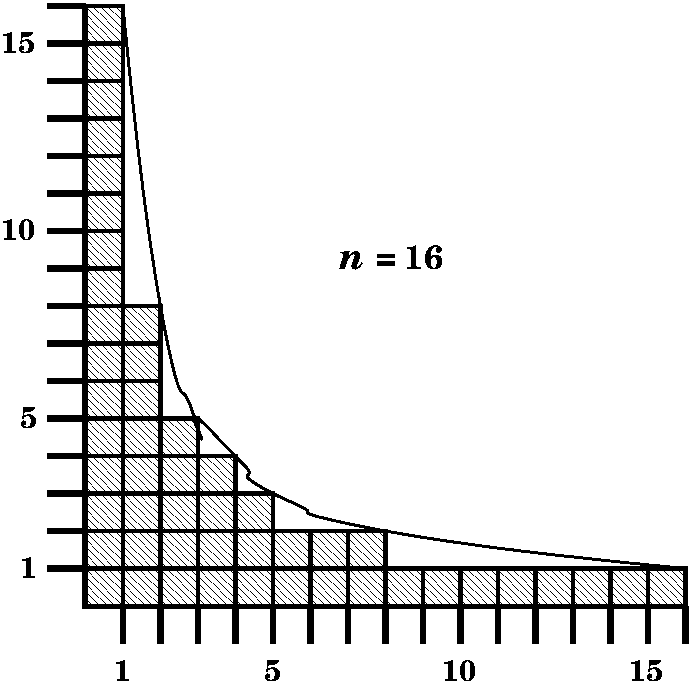
\includegraphics[scale=0.4]{pairing-hyp.pdf}
\caption{{\it The aggregate set of positions of tables having $16$ or
fewer position.}
\label{f.hyp}}
\end{figure}

   

\ignore{*****************
\noindent {\em Additive pairing functions}
%
The study in \cite{Rosenberg02} focuses on pairing functions that are
{\it additive}: Assign each row $v$ a {\it base task-index} $B_v$ and
a {\it stride} $S_v$.  Then use the formula
\[ \t(v, t) \ = \ B_v + (t-1) S_v \]
to map $\N^+ \times \N^+$ bijectively onto $\N^+$.

{\em A methodology for designing {\em additive} pairing functions.}
%
Easily, any additive pairing function must have infinitely many
distinct strides; i.e., $S_x$, viewed as a function of $x$, must have
infinite range.  Despite this, that there do exist easily computed
additive pairing functions.  One strategy for designing such pairing
functions builds on the following well-known property of the set \O\/
of positive odd integers.

\begin{lemma}[\cite{NivenZ80}]
\label{l.odds}
For any positive integer $c$, every odd integer can be written
in precisely one of the $2^{c-1}$ forms:
\[ 2^c n +1, \ 2^c n +3, \ 2^c n +5, \ldots, \ 2^c n + (2^c -1), \]
for some nonnegative integer $n$.
\end{lemma}

\noindent
One builds on Lemma~\ref{l.odds} to construct additive pairing
functions (APFs) in the following manner.

\paragraph{\underline{Procedure}} {
\sf APF-Constructor}($\t$) \\
/*Construct an APF $\t$*/
\begin{description}
\item[Step 1.]
Partition the set of row-indices into {\it groups} whose sizes are
powers of 2 (with any desired mix of equal-size and distinct-size
groups).  Order the groups linearly in some (arbitrary) way.
\end{description}
/*One can now talk unambiguously about group 0 (whose members share
{\it group-index} $g=0$), group 1 (whose members share group-index
$g=1$), and so on.*/
\begin{description}
\item[Step 2.]
Assign each group a distinct copy of the set \O, as well as a {\it
copy-index} $\kappa(g)$ expressed as a function of the group-index
$g$.

\item[Step 3.]
Allocate group $g$'s copy of \O\/ to its members via the $(c =
\kappa(g))$ instance of Lemma~\ref{l.odds}, using the multiplier $2^g$
as a {\it signature} to distinguish group $g$'s copy of the set \O\/
from all other groups' copies.
\end{description}
One can specify the procedure's APFs in a computationally friendly
way.

{\em An explicit expression for $\t$.}
If we denote the $2^{\kappa(g)}$ rows of group $g$ as $x_{g,1}$,
$x_{g,2}$, \ldots, $x_{g,2^{\kappa(g)}}$, then for all $i \in \{ 1, 2,
\ldots, 2^{\kappa(g)} \}$,
\begin{equation}
\label{e.define.t}
\t(x_{g,i}, y) \ \eqdef \
2^g \left[ 2^{1 + \kappa(g)}(y-1) +
	(2x_{g,i} +1 \bmod 2^{1 + \kappa(g)}) \right]
\end{equation}

\begin{theorem}
\label{t.define.ataf}
Any function $\t: \N^+ \times \N^+ \leftrightarrow \N^+$ that is
designed via Procedure {\small\sf APF-Constructor}, hence is of the
form (\ref{e.define.t}), is a valid additive pairing function whose
base row-entries and strides satisfy
\begin{equation}
\label{e.genl.b.s}
B_x \ \leq \
S_x \ =    \ \t(x, y+1) - \t(x,y) \ = \ 2^{1 + g + \kappa(g)}.
\end{equation}
\end{theorem}
*********************}



\subsection{Numerals}\index{numerals}
\label{sec:Numerals}

We can identify distinct families of {\em operational}
numerals,\index{numerals!operational} i.e., numerals that allow one to
do things such as perform arithmetic (add, multiply, etc.).

**THOUGHTS*******
series expansions, strings created by a positional number system, and
hybrids built on positional systems such as ``scientific notation''.
*************


Of course, we are all familar with certain numbers that have {\em
  non-operational} names that we use all the time.  Notable among
these are (using terminology that anticipates future sections and
chapters):
\begin{itemize}
\item
$\pi$: the ratio of the circumference of a circle to its diameter;
  $\pi \approx 3.141592653 \ldots$
\item
$e$: Euler's constant; the base of ``natural'' logarithms: $e \approx
  2.718281828 \ldots$
\item
$i$: the name of the number whose square is $-1$; $i$ is appended to
  the real numbers in order to ``complete'' them to the complex
  numbers, within which system every polynomial of degree $n$ has $n$
  roots.
\end{itemize}

\medskip

%\addcontentsline{toc}{paragraph}{A. Positional number systems}
\paragraph{\small\sf A. Positional number systems}
\index{positional number system}

The most common way of forming numerals is via strings over a {\it
  number base}.\index{positional number system!base of the system}  
%
We begin with an integer $b>1$ that will serve as our base, and we
define the set $B_b = \{ 0, 1, \ldots, b-1\}$ of {\it digits in base
  $b$}.\index{positional number system!digits in base $b$}
%
To aid legibility, {\em within the context of base-$b$ positional
  numerals}, we denote the digit $b-1$ as a single character,
$\bar{b}$.\index{$\bar{b}$: the digit $b-1$ in base $b$}
%
We then form base-$b$ numerals in the following way.\index{positional
  number system!base-$b$ numerals}
%
This formation builds on {\em geometric sums}, a mathematical
structure that we shall learn to manipulate, evaluate, and compute
with in Section~\ref{sec:geometric-sums}.

A base-$b$ numeral is a string having three sections.
\begin{enumerate}
\item
The numeral begins with its {\em integral part},\index{positional
  number system!integral part of a numeral}
%
which is a finite string of digits from $B_b$: $\alpha_n \alpha_{n-1}
\cdots \alpha_1 \alpha_0$.

The base-$b$ number represented by the numeral's integral
part\index{positional number system!numerical value of integral part}
is\footnote{Our underlined notation for the numerical value of a
  numeral is not common, but we find it convenient.}
\[
\underline{\alpha_n \alpha_{n-1}\cdots \alpha_1 \alpha_0}
\ \ \eqdef \ \
\sum_{i=0}^n \alpha_i \cdot b^i
\]

\item
The numeral continues with a single occurrence of the {\it
  radix point}\index{positional number system!radix point ``$.$''}
``$.$''
\item
The numeral ends with its {\em fractional part},\index{positional
  number system!fractional part of a numeral}
%
which is a string---{\em finite or infinite}--- of digits from $B_b$:
$\beta_0 \beta_1 \beta_2 \cdots$.

The base-$b$ number represented by the numeral's fractional part
is\index{positional number system!numerical value of fractional part}
\[
\underline{. \beta_0 \beta_1 \beta_2 \cdots}
\ \ \eqdef \ \
\sum_{j\geq 0} \beta_j \cdot b^{-j}
\]
\end{enumerate}
In summary, then, the base-$b$ number represented by the numeral
$\alpha_n \alpha_{n-1} \cdots \alpha_1 \alpha_0                  
. \beta_0 \beta_1 \beta_2 \cdots$ 
is\index{positional number system!numerical value of numeral}
\[
\underline{\alpha_n \alpha_{n-1} \cdots \alpha_1 \alpha_0                  
. \beta_0 \beta_1 \beta_2 \cdots}
\ \ \eqdef \ \
\sum_{i=0}^n \alpha_i \cdot b^i
\ + \ \sum_{j\geq 0} \beta_j \cdot b^{-j}.
\]
By prepending a ``negative sign'' (or, ``minus sign'') $-$ to a
numeral or a number, one renders the thus-embellished entity as
negative.

\bigskip

%\addcontentsline{toc}{paragraph}{B. Scientific notation}
\paragraph{\small\sf B. Scientific notation}
\index{Scientific notation}

The finite numerals in subsection A are all ``exact'' in the sense
that changing any digit changes the value of the named number.  We
turn now to a class of numerals that abjure this ``exactness'' for the
sake of expedience.  There are a few reasons that one might be willing
to do this.

\begin{itemize}
\item
WHY SCIENTIFIC NOTATION
\end{itemize}

\addcontentsline{toc}{paragraph}{C. Exact arithmetic}





\section{Arithmetic and Its Laws}\index{laws of arithmetic}
\label{sec:Arithmetic-Tools+Laws}

Numbers are {\it adjectives}\index{number!as adjective}---you have
five apples and three oranges---but in contrast to adjectives that are
purely descriptive---the red ball, the big dog---numbers can be {\em
  manipulated},\index{number!as {\em manipulable} adjective} using the
tools of {\it arithmetic}.

\subsection{The Tools of Arithmetic}
\label{sec:arithmetic-tools}

The basic tools of arithmetic reside in a small set of operations,
together with two special integers that play important roles with
respect to the operations.  Since these entities are so tightly
intertwined, we discuss them simultaneously.

\smallskip

\noindent {\small\sf Two special integers}
%
The integers zero ($0$)\index{number!zero ($0$)} and one
($1$),\index{number!one ($1$)} play special roles within all four of
the classes of numbers we have described.

\smallskip

\noindent {\small\sf  The operations of arithmetic}\index{arithmetic!basic operations}
%
Arithmetic on the four classes of numbers that we have described is
built upon a rather small repertoire of operations.  When we say that
an operation produces a number ``of the same sort'', we mean that it
produces
\begin{itemize}
\item
an integer result from integer arguments;
\item
a rational (number) result from rational (number) arguments;
\item
a real (number) result from real (number) arguments;
\item
a complex (number) result from complex (number) arguments;
\end{itemize}
The fundamental operations on numbers are, of course, familiar to the
reader.  Our goal in discussing them is to stress the laws that govern
the operations.  Along the way, we also introduce a few operations
that are less familiar but no less important.

\subsubsection{Unary (single-argument) operations}

\addcontentsline{toc}{paragraph}{A. Negating and reciprocating numbers}
\noindent {\small\sf A. Negating and reciprocating numbers.}
\index{arithmetic!basic operations!negation}
%
\noindent {\it i. The operation of {\em negation}}:
\index{arithmetic!basic operations!negating}
\begin{itemize}
\item
is a {\em total function} on the sets $\Z, \Q, \R, \C$.  It replaces
a number $a$ by its {\em negative},
\index{number!negative}
a number of the same sort, denoted $-a$.
\item
is a {\em partial function} on the nonnegative subsets
of $\Z, \Q, \R, \C$.  It replaces a number $a$ by its negative, $-a$,
whenever both $a$ and $-a$ belong to the nonnegative subset being
operated on.
\end{itemize}
Zero ($0$) is the unique {\it fixed point}\index{function!fixed
  point}\index{arithmetic!negation!fixed point} of the operation,
meaning that $0$ is the unique number $a$ such that $a = -a$.

\medskip

\noindent {\it ii. The operation of {\em reciprocation}}:
\index{arithmetic!basic operations!reciprocal}
\begin{itemize}
\item
\index{arithmetic!basic operations!reciprocating}
is a {\em total function} on the sets $\Q, \R, \C$, which replaces each
number $a$ by its {\em reciprocal}, 
\index{number!reciprocal}
a number of the same sort, denoted $1/a$ or $\displaystyle {1 \over
  a}$.  We shall employ whichever notation enhances legibility.

\item
is {\em undefined} on every integer $a$ except for $1$.
\end{itemize}

\medskip

\addcontentsline{toc}{paragraph}{B. Floors, ceilings, magnitudes}
\noindent {\small\sf B. Floors, ceilings, magnitudes.}
\index{arithmetic!basic operations!floor}
\index{arithmetic!basic operations!ceiling}
\index{arithmetic!basic operations!absolute value}
\index{arithmetic!basic operations!magnitude}

\noindent {\it i. The operations of {\em taking floors and ceilings}}
are total operations on the sets $\N, \Z, \Q, \R$.
\begin{itemize}
\item
The {\it floor} of a number $a$, also called {\it the integer part}
\index{arithmetic!basic operations!integer part of a number}
\index{arithmetic!basic operations!floor of a number}
of $a$, denoted $\lfloor a \rfloor$, is the largest integer that does
not exceed $a$; i.e.,:
\[
\lfloor a \rfloor \ \eqdef \ \max_{b \in {\mathbb{N}}} \Big[ b \ \leq a \Big]
\]
\item
The {\it ceiling} of a number $a$
\index{arithmetic!basic operations!ceiling of a number}
of $a$, denoted $\lceil a \rceil$, is the smallest integer that is 
not smaller than $a$:
\[
\lceil a \rceil \ \eqdef \ \min_{b \in {\mathbb{N}}} \Big[ b \ \geq a \Big]
\]
\end{itemize}
Thus, the operations of taking floors and ceilings are two ways to
{\em round} rationals and reals to their ``closest''
integers.\index{arithmetic!basic operations!rounding to ``closest'' integer}

\medskip

\noindent {\it ii. The operations of taking {\em absolute values/magnitudes}}:
\index{arithmetic!basic operations!absolute value, magnitude}
%
Let $a$ be a real number.  The {\it absolute value}, or, {\it
  magnitude}, of $a$, denoted $|a|$ equals either $a$ or $-a$,
whichever is positive.  For a complex number $a$, the definition of
$|a|$ is more complicated: it is a measure of $a$'s ``distance'' from
the ``origin'' complex number $0 + 0 \cdot i$.  In detail:
\[
|a| \ = \ \left\{
\begin{array}{cl}
a & \mbox{ if } \ [a \in \R] \ \ \mbox{ and } [a \geq 0] \\
-a & \mbox{ if } \ [a \in \R] \ \ \mbox{ and } [a < 0] \\
\sqrt{b^2 + c^2} &  \mbox{ if } \ [a \in \C]  \ \ \mbox{ and } [a = (b+ci)]
\end{array}
\right.
\]

\medskip

\addcontentsline{toc}{paragraph}{C. Factorials (of nonnegative integers)}
\noindent {\small\sf C. Factorials (of nonnegative integers).}
\index{arithmetic!basic operations!factorial (of a nonnegative integer)}
%
The {\it factorial} of a nonnegative integer $n \in \N$, which is
commonly denoted $n!$,
\index{arithmetic!basic operations!$n!$: factorial of $n \in \N$}
\index{arithmetic!basic operations!factorial of nonnegative integer}
is the function defined via the following recursion.
\begin{equation}
\label{eq:n-factorial-recursion}
\mbox{\sc fact}(n) \ = \ \left\{
\begin{array}{cl}
1 & \mbox{  if } \ n=0 \\
n \cdot \mbox{\sc fact}(n-1) & \mbox{  if } \ n>0
\end{array}
\right.
\end{equation}
By ``unwinding'' the recursion in (\ref{eq:n-factorial-recursion}),
one finds that, for all $n \in \N$,
\begin{equation}
\label{eq:n-factorial-direct}
n! \ = \ \mbox{\sc fact}(n) \ = \ 
n \cdot (n-1) \cdot (n-2) \cdot \cdots \cdot 2 \cdot 1
\end{equation} 
A $3$-step inductive argument validates this ``unwinding'':
\begin{enumerate}
\item
If $n =0$, then {\sc fact}$(n) = 1$, by definition
(\ref{eq:n-factorial-recursion}).
\item
Assume, for induction, that the expansion in
(\ref{eq:n-factorial-direct}) is valid for a given $k \in N$:
\[ \mbox{\sc fact}(k) \ = \ k \cdot (k-1) \cdot (k-2) \cdot \cdots
\cdot 2 \cdot 1 \] 
\item
Then:
\[
\begin{array}{lclll}
\mbox{\sc fact}(k+1) & = & (k+1) \cdot \mbox{\sc fact}(k)
  & & \mbox{by (\ref{eq:n-factorial-recursion})} \\
  & = &
(k+1) \cdot k \cdot (k-1) \cdot (k-2) \cdot \cdots \cdot 2 \cdot 1
  & & \mbox{by induction}
\end{array}
\]
\end{enumerate}


\subsubsection{Binary (two-argument) operations}
\label{sec:binary-operators}

%\addcontentsline{toc}{paragraph}{A. Addition and Subtraction}
\paragraph{\small\sf A. Addition and Subtraction.}
\index{arithmetic!basic operations!addition}
\index{arithmetic!basic operations!subtraction}
%
The operation of {\it addition}\index{arithmetic!addition} is a {\em
  total function} that replaces any two numbers $a$ and $b$ by a
number of the same sort.  The resulting number is the {\em sum of $a$
  and $b$}\index{arithmetic!addition!sum} and is denoted $a+b$.

\noindent
The operation of {\it subtraction}\index{arithmetic!subtraction} is a
{\em total function} on the sets $\Z, \Q, \R, \C$, which replaces any
two numbers $a$ and $b$ by a number of the same sort.  The resulting
number is the {\em difference of $a$ and $b$}
\index{arithmetic!subtraction!difference} and is denoted $a-b$.  On
the nonnegative subsets of the sets $\Z, \Q, \R, \C$---such as $\N$,
which is the largest nonnegative subset of $\Z$---subtraction is a
{\em partial function}, which is defined only when $a \geq b$.

Subtraction can also be defined as follows.  For any two numbers $a$
and $b$, {\em the difference of $a$ and $b$ is the sum of $a$ and the
  negation of $b$}; i.e.,
\[ a-b \ = \ a + (-b) \]

{\em The special role of $0$ under addition and subtraction.}
%
The number $0$ is the {\it identity} under addition and
  subtraction.\index{number!additive identity}\index{number!identity
  under addition}\index{identity!additive}
%
This means that, for all numbers $a$,
\[ a+0 \ = \ a-0 \ = \ a. \]

{\em The special role of $1$ under addition and subtraction.}
%
For any integer $a$, there is no integer between $a$ and $a+1$ or
between $a-1$ and $a$.  For this reason, on the sets $\Z$ and $\N$,
one often singles out the following special cases of addition and
subtraction, especially in reasoning about situations that are indexed
by integers.  Strangely, these operations have no universally accepted
notations.
\begin{itemize}
\item
The {\it successor} operation\index{arithmetic!integers!successor} is
a {\em total function} on both $\N$ and $\Z$, which replaces an
integer $a$ by the integer $a+1$.
\item
The {\it predecessor} operation\index{arithmetic!integers!predecessor}
is a {\em total function} on $\Z$, which replaces an integer $a$ by
the integer $a-1$.  It is a {\em partial function} on $\N$, which is
defined only when the argument $a$ is positive (so that $a-1 \in \N$).
\end{itemize}

The operations of addition and subtraction are said to be {\em
  inverse operations}\index{arithmetic!integers!additive inverse}
\index{arithmetic!integers!addition and subtraction are mutually
  inverse} of each other because each can be used to ``undo'' the
other:
\[
a \ = \ (a+b) -b \ = \ (a-b) +b
\]

\medskip

\addcontentsline{toc}{paragraph}{B. Multiplication and Division}
\noindent {\small\sf B. Multiplication and Division}.
\index{arithmetic!basic operations!multiplication}
\index{arithmetic!basic operations!division}
%
The operation of {\it multiplication}\index{arithmetic!multiplication}
is a {\em total function} that replaces any two numbers $a$ and $b$ by
a number of the same sort.  The resulting number is the {\em product
  of $a$ and $b$}\index{arithmetic!multiplication!product} and is
denoted either $a \cdot b$ \index{arithmetic!multiplication!$a \cdot  b$}
or $a \times b$.\index{arithmetic!multiplication!$a \times b$}
We shall usually favor the former notation, except when the latter
enhances legibility.

The operation of {\it division}\index{arithmetic!division} is a {\em
  partial function} on all of our sets of numbers.  Given two numbers
$a$ and $b$, the result of dividing $a$ by $b$---{\em when that result
  is defined}---is the {\it quotient of $a$ by $b$}
\index{arithmetic!division!When is $a/b$ defined?}
\index{arithmetic!division!quotient}
\index{arithmetic!division!quotient!$a/b$}
\index{arithmetic!division!quotient!$a \div b$}
\index{arithmetic!division!quotient!${a \over b}$}
and is denoted by one of the following three notations: $a/b$, $a \div
b$, $\displaystyle{a \over b}$.  The {\it quotient of $a$ by $b$} is
defined precisely when {\em both}

\noindent
\hspace*{.35in}(1) $b \neq 0$: one can never divide by $0$ \\
\hspace*{.35in}{\em and} \\
\hspace*{.35in}(2) there exists a number $c$ such that $a = b \cdot c$.

\noindent
Assuming that condition (1) holds, {\em condition (2) always holds
  when $a$ and $b$ belong to $\Q$ or $\R$ or $\C$}.

Division can also be defined as follows.  For any two numbers $a$
and $b$, {\em the quotient of $a$ and $b$ is the product of $a$ and the
reciprocal of $b$} (assuming that the latter exists); i.e.,
\[ a/b \ = \ a \cdot (1/b). \]
Computing reciprocals of nonzero numbers in $\Q$ and $\R$ is standard
high-school level fare; computing reciprocals of nonzero numbers in
$\C$ requires a bit of calculational algebra which we do not cover.
For completeness, we note that the reciprocal of the {\em nonzero}
complex number $a + bi \in \C$ is the complex number $c+di$ where
\[ c \ = \ \frac{a}{a^2 + b^2} \ \ \ \ \
\mbox{ and } \ \ \ \ \
d \ = \ \frac{-b}{a^2 + b^2}.
\]

{\em The special role of $1$ under multiplication and division.}
%
The number $1$ is the {\it identity} under the operations of
multiplication and division.\index{number!multiplicative
  identity}\index{number!identity under
  multiplication}\index{identity!multiplicative}
%
This means that, for all numbers $a$,
\[ a \cdot 1 \ = \ a \cdot (1/1) \ = \ a. \]

{\em The special role of $0$ under multiplication and division.}
%
The number $0$ is the {\it annihilator} under
multiplication.\index{multiplicative annihilator} This means that, for
all numbers $a$
\[ a \cdot 0 \ = \ 0. \]

The operations of multiplication and division are said to be {\em
  inverse operations}\index{arithmetic!integers!multiplicative
  inverse} \index{arithmetic!integers!multiplication and division are
  mutually inverse} because, when both operations can be applied, each
can be used to ``undo'' the other:
\[ a = (a \cdot b) \div b \ = \ (a \div b) \cdot b.  \]

\medskip

%\addcontentsline{toc}{paragraph}{C. Binomial coefficients and Pascal's triangle}
\paragraph{\small\sf C. Binomial coefficients and Pascal's triangle}
\index{arithmetic!basic operations!binomial coefficient}

We close our catalogue of arithmetic operations with a binary
operation on\footnote{In advanced contexts, one encounters binomial
  coefficients with non-integer arguments.}~$\N \times \N$.

Let $n$ and $k \leq n$ be nonnegative integers (i.e., elements of
$\N$).  The {\it binomial coefficient} denoted either as
$\displaystyle {n \choose k}$ or as $\Delta_{n,k}$, is the number
\index{binomial coefficients}
\begin{equation}
\label{eq:binom-coeff}
\Delta_{n,k} \ = \
{n \choose k} \ \eqdef \ \frac{n!}{k!(n-k)!} \ = \
\frac{n(n-1)(n-2) \cdots (n-k+1)}{k (k-1)(k-2) \cdots 1}
\end{equation}
Many of the secrets of these wonderful numbers---including the fact
that they are {\em integers}---can be deduced from the following
results.

\begin{prop}
\label{thm:manipulate-binom-coeff}
For all $n, k \in \N$ with $k \leq n$:

{\rm (a)} The symmetry rule:
\index{binomial coefficients!symmetry rule}
\begin{equation}
\label{eq:symmetry-binom-coeff}
{n \choose k} \ = \ {n \choose {n-k}}
\end{equation}

{\rm (b)} The addition rule:
\index{binomial coefficients!addition rule}
\begin{equation}
\label{eq:add-binom-coeff}
{n \choose k} \ + \ {n \choose {k+1}} \ = \ {{n+1} \choose {k+1}}
\end{equation}
\end{prop}

\begin{proof}
($a$)
We verify equation (\ref{eq:symmetry-binom-coeff}) by
(\ref{eq:binom-coeff}) plus the commutativity of multiplication (see
Section~\ref{sec:Arithmetic-Laws}),
\begin{eqnarray*}
{n \choose k} & = & \frac{n!}{k!(n-k)!} \\
              & = & \frac{n!}{(n-k)!k!} \\
              & = & {n \choose {n-k}}
\end{eqnarray*}

\noindent ($b$)
We verify equation (\ref{eq:add-binom-coeff}) by explicitly adding the
fractions exposed by (\ref{eq:binom-coeff}):
\begin{eqnarray*}
{n \choose k} \ + \ {n \choose {k+1}}
  & = &
\frac{n!}{k!(n-k)!} \ + \ \frac{n!}{(k+1)!(n-k-1)!} \\
  & = &
n! \cdot \frac{(k+1) + (n-k)} {(k+1)!(n-k)!} \\
  & = & 
\frac{(n+1)!}{(k+1)!(n-k)!} \\
  & = &
{{n+1} \choose {k+1}} \hspace*{2in} \qed
\end{eqnarray*}

Extrapolating from Proposition~\ref{thm:manipulate-binom-coeff}, we now
present {\it Pascal's triangle}, named in honor of
\index{Pascal's triangle}
\index{Pascal, Blaise}
the French polymath Blaise Pascal.  Fig.~\ref{fig:pascal-triangle}
provides a ``prefix'' of this famed array of integers, for $n,k \leq
5$.
\begin{figure}[htb]
\[
\begin{array}{c||r|r|r|r|r|r|r}
{\displaystyle {n \choose k}} & k=0 & k=1 & k=2 & k=3 & k=4 & k=5 &\ldots \\
\hline
\hline
n=1 & 1 & 1 &    &    &    &   & \ldots \\
\hline
n=2 & 1 & 2 & 1  &    &    &   & \ldots \\
\hline
n=3 & 1 & 3 & 3  & 1  &    &   & \ldots \\
\hline
n=4 & 1 & 4 & 6  & 4  & 1  &   & \ldots \\
\hline
n=5 & 1 & 5 & 10 & 10 & 5  & 1 & \ldots \\
\hline
\vdots &\vdots &\vdots &\vdots &\vdots &\vdots &\vdots &\ddots
\end{array}
\]
\caption{A ``prefix'' of Pascal's Triangle, for $n,k \leq 5$.}
\label{fig:pascal-triangle}
\end{figure}
The formation rule of the array is:
\begin{description}
\item[\sf Formation rule for Pascal's triangle:]
% 
{\it The entry at (row $n+1$, column $k+1$) is the sum of the entries
  at (row $n$, column $k$) and (row $n$, column $k+1$).}
\end{description}
\qed
\end{proof}


If you compare the formation rule for Pascal's triangle with equation
(\ref{eq:add-binom-coeff}), then you may anticipate the following
result.

\addcontentsline{toc}{paragraph}{-- A fun result: Pascal's triangle
  and the binomial coefficients}

\begin{prop}
\label{thm:pascal-binom}
The entries of Pascal's triangle are the binomial coefficients.
Specifically, for all $n,k$, the entry at (row $n$, column $k$) of the
Triangle is $\displaystyle {n \choose k}$.
\end{prop}

\begin{proof}
We note by observation and direct calcullation (see
Fig.~\ref{fig:pascal-triangle}) that the proposition is true for $n =
1$ and $k \in \{0, 1\}$.  A simple double induction

\noindent
****************** \\
induction on $n$, then for each value of $n$ on $k \leq n$ \\
SHOULD WE SPELL THIS OUT IN DETAIL?  GIVE AS AN EXERCISE? \\
******************

\noindent
verifies that every binomial coefficient appears in the Triangle and
every Triangle entry is a binomial coefficient.  \qed
\end{proof}

\medskip

\addcontentsline{toc}{paragraph}{-- A fun result: Binomial
  coefficients are integers}

\begin{prop}
\label{thm:binomcoeff-integer}
Every binomial coefficient is an integer.
\end{prop}

\begin{proof}
Since every entry in Pascal's triangle is obtained from integers via
repeated additions, this result follows from
Proposition~\ref{thm:pascal-binom}.  \qed
\end{proof}

\bigskip

Binomial coefficients are indispensable when studying myriad topics
related to {\em counting}, such as:
\begin{itemize}
\item
what are the relative likelihoods of various $5$-card deals from a
fair $52$-card deck?
\item
What is the likelihood of observing $15$ {\sc head}s and $25$ {\sc
  tail}s in $40$ flips of a fair coin?
\item
What are the comparative operation-count costs of Merge-Sort and
Quick-Sort when sorting $n$ keys; cf.~\cite{CLRS}?

\end{itemize}
We shall, therefore, see a lot more about binomial coefficients in
Section~\ref{sec:powers+polynolmials} and Chapter~\ref{ch:prob-stat}.
With each subsequent encounter, our respect for these numbers will
grow.


\subsection{The Laws of Arithmetic, and applications}
\index{arithmetic!basic laws}
\label{sec:Arithmetic-Laws}

The student should understand the following laws of arithmetic on the
reals, rationals, and reals---and be able to employ them cogently in
rigorous argumentation.

\medskip

\addcontentsline{toc}{paragraph}{A. The commutative law}
\noindent {\small\sf A. The commutative law.}
\index{commutative law!arithmetic}
\index{commutative law!addition}
\index{commutative law!multiplication}
\index{arithmetic!commutative law}
%
For all numbers $x$ and $y$:
\[
\begin{array}{llc}
\mbox{\it for addition:}
  & & x+y \ = \ y+x \\
\mbox{\it for multiplication:}
  & & x \cdot y \ = \ y \cdot x
\end{array}
\]

\medskip

\addcontentsline{toc}{paragraph}{B. The associative law}
\noindent {\small\sf B. The associative law}
\index{associative law for arithmetic}
\index{arithmetic!associative law}
%
For all numbers $x$, $y$, and $z$,
\[ (x+y)+z \ = \ x+(y+z) \ \ \ \mbox{\bf and } \ \ 
x\cdot (y\cdot z) 
(x \cdot y) \cdot z \ = \ x\cdot (y\cdot z). \] 
This allows one, for instance, to write strings of additions or of
multiplications without using parentheses for grouping.

\medskip

\addcontentsline{toc}{paragraph}{C. The distributive law}
\noindent  {\small\sf C. The distributive law.}
\index{distributive law for arithmetic}
\index{arithmetic!distributive law}
%
For all numbers $x$, $y$, and $z$,
\begin{equation}
\label{eq:distr-law}
x \cdot (y + z) \ = \ (x \cdot y) + (x \cdot z).
\end{equation}
One commonly articulates this law as, ``{\em Multiplication
  distributes over addition.}''


One of the most common uses of the distributive law reads equation
(\ref{eq:distr-law}) ``backwards,'' thereby deriving a formula for
{\em factoring} \index{arithmetic!factoring} complex expressions that
use both addition and multiplication.

Easily, addition does {\em not} distribute over multiplication; i.e.,
in general, $x + y \cdot z \ \neq \ (x+y) \cdot (x+z)$.  Hence, when
we see ``$x + y \cdot z$'', we know that the multiplication is
performed before the addition.  In other words, {\em Multiplication
  takes priority over addition.}  \index{arithmetic!priority of
  multiplication over addition} This priority permits us to write the
righthand side of (\ref{eq:distr-law}) without parentheses, as in
\[ x \cdot (y + z) \ = \ x \cdot y + x \cdot z. \]

Via multiple invocations of the preceding laws, we can derive a recipe
for multiplying complicated expressions.  We illustrate this via the
``simplest'' complicated expression, $(a+b) \cdot (c+d)$.

\begin{prop}
\label{prop:(a+b)(c+d)}
For all numbers $a, b, c, d$:
\begin{equation}
\label{eq:(a+b)(c+d)}
(a+b) \cdot (c+d) \ = \ a \cdot c + a \cdot d + b \cdot c + b \cdot d
\end{equation}
\end{prop}

\begin{proof}
Note first that because multiplication takes priority over addition,
the absence of parentheses in expressions such as
(\ref{prop:(a+b)(c+d)}) does not jeopardize unambiguity.  Our proof of
the proposition invokes the laws we have just enunciated multiple
times.
\[
\begin{array}{lclll}
(a+b) \cdot (c+d) & = & (a+b) \cdot c \ + \ (a+b) \cdot d
& & \mbox{distributive law} \\ 
  & = & c \cdot (a+b) \ + \ d \cdot (a+b)
& & \mbox{commutativity of multiplication} \ (2 \times) \\
  & = & c \cdot a + c \cdot b + d \cdot a + d \cdot b 
& & \mbox{distributive law} \ (2 \times) \\
  & = & a \cdot c + b \cdot c + a \cdot d + b \cdot d
& & \mbox{commutativity of multiplication} \ (4 \times) \\
  & = &  a \cdot c + a \cdot d + b \cdot c + b \cdot d
& & \mbox{commutativity of addition}
\end{array}
\]
\qed
\end{proof}


We close our short survey of the laws of arithmetic with the following
important two-part law.
\begin{itemize}
\item
{\it The law of inverses}.\index{inverse laws for
  arithmetic}\index{laws of arithmetic!inverse laws}
%
  \begin{itemize}
  \item
Every number $x$ has an {\em additive inverse},\index{additive inverse}
i.e., a number $y$ such that $x+y =0$.  This inverse is $x$'s {\it
  negative} $-x$.\index{additive inverse!negative as additive inverse}
  \item
Every {\em nonzero} number $x \neq 0$ has a {\em multiplicative
  inverse},\index{multiplicative inverse} i.e., a number $y$ such that
$x \cdot y = 1$.  This inverse is $x$'s {\it reciprocal},
$1/x$.\index{multiplicative inverse!reciprocal as multiplicative inverse}
  \end{itemize}
\end{itemize}

We close this section with another of our ``fun'' propositions.

\addcontentsline{toc}{paragraph}{-- A fun result: A ``trick'' for
  squaring some integers}

\begin{prop}
\label{thm:75x65=4925}
Let $n$ be any number that has a $2$-digit decimal of the form $\delta
5$, where $\delta \in \{ 0,1,2,3,4,5,6,7,8,9 \}$,
so that
\[ n \ = \ 10 \cdot \delta + 5
\]
Then 
\[ n^2 \ = \ 100 \cdot \delta \cdot (\delta+1) + 25. \]
In other words, one obtains a base-$10$ numeral for $n^2$ by
multiplying $\delta$ by $\delta +1$ and appending $25$ to the product.
\end{prop}

\noindent
Examples of Proposition ~\ref{thm:75x65=4925} include
$25^2 = 625$ (because $2 \cdot 3 = 6$) and $75^2 = 5625$ (because $7
\cdot 8 = 56$).

\begin{proof} (for general $\delta$).
%
We invoke Proposition~\ref{prop:(a+b)(c+d)} and the distributive law.
\[
\begin{array}{lclll}
n^2 & = & (10 \cdot \delta + 5)^2 & & \mbox{Given} \\
    & = & 100 \cdot \delta^2 \ + \ 100 \cdot delta \ + \ 25
              & & \mbox{the proposition} \\
    & = & 100 \cdot (\delta^2 \ + \ \delta) \ + \ 25
              & & \mbox{factoring: distributive law} \\
    & = & 100 \cdot \delta \cdot (\delta + 1) \ + \ 25
              & & \mbox{factoring: distributive law} \\
\end{array}
\]
\qed
\end{proof}


\subsection{Rational Arithmetic: A Worthwhile Exercise}
\label{sec:Rational-arithmetic}
\index{number!rational!arithmetic}

In Section~\ref{sec:rationals} we defined the rational numbers and
reviewed why they were needed to compensate for the general lack of
multiplicative inverses in the integers.  But we did not review how to
perform arithmetic on the elements of the set $\Q$.  We correct this
shortcoming now.  Of course, the reader will have encountered rational
arithmetic long ago---but we are now reviewing the topic in order to
provide the reader with a set of worthwhile exercise to reinforce the
mathematical thinking whose presentation is our main goal.

\medskip

The rational numbers build their rules for arithmetic upon the
corresponding rules for integers.  For all $p/q$ and $r/s$ in $\Q$:
\[
\begin{array}{|llcl|}
\hline
\mbox{\small\sf Addition:} & 
{\displaystyle
{p \over q} + {r \over s} }
  & = &
{\displaystyle
 \frac{p \cdot s + r \cdot q}{q \cdot s} }  \\
 & & & \\
\mbox{\small\sf Subtraction:} &
{\displaystyle
{p \over q} + {r \over s} }
  & = & 
{\displaystyle
{p \over q} + {(-r) \over s} } \\
 & & & \\
\mbox{\small\sf Multiplication:} &
{\displaystyle
{p \over q} \cdot {r \over s} }
  & = & 
{\displaystyle
\frac{p \cdot r}{r \cdot s} } \\
  & & & \\
\mbox{\small\sf Division:} &
{\displaystyle
{p \over q} \div {r \over s} }
  & = &
{\displaystyle
{p \over q} \cdot {s \over r} } \\
\hline
\end{array}
\]

It is worth verifying that rational arithmetic as thus defined behaves
in the required manner; in particular that rational arithmetic:
\begin{itemize}
\item
works correctly when the argument rational numbers are, in fact,
integers, i.e., when $q = s = 1$ in the preceding table.
\item
treats the number $0$ appropriately, i.e., as an additive identity and
a multiplicative annihilator; cf., Sections~\ref{sec:arithmetic-tools}
and~\ref{sec:Arithmetic-Laws}.
\item
obeys the required laws; cf., Section~\ref{sec:Arithmetic-Laws}.

Verifying the distributivity of rational multiplication over rational
addition will be a particularly valuable exercise because of the
required amount of manipulation.
\end{itemize}

\section{Basic Algebraic Concepts and Their Manipulations}

\subsection{Powers and polynomials}
\label{sec:powers+polynolmials}

\subsubsection{Raising a number to a power.}
\label{sec:x-toa-power}
A conceptually powerful notational construct is the operation of {\it
  raising a number to a power:}\index{raising a number to a power}
%
For real numbers $a$ and $b$, the {\it $b$th power} of $a$, denoted
$a^b$ is defined by the system of equations
\begin{equation}
\label{eq:power-def}
\begin{array}{llll}
\mbox{for all numbers $a>0$} & & & a^0 = 1 \\
 & & & \\
\mbox{for all numbers $a, b, c$} & & & a^b \cdot a^c = a^{b+c}.
\end{array}
\end{equation}
This deceptively simple definition has myriad consequences which we
often take for granted.
\begin{itemize}
\item
For all numbers $a>0$, the number $a^0 = 1$.

This follows (via cancellation) from (\ref{eq:power-def}) via the fact
that
\[ a^b \cdot a^0 \ = \ a^{b+0} \ = \ a^b \ = \ a^b \cdot 1.  \]

\item
For all numbers $a >0$, the number $a^{1/2}$\index{$a^{1/2}$: the
  square root of number $a$}
is the {\it square root} of $a$,\index{square root}
i.e., $a^{1/2}$ is the (unique, via cancellation) number $b$ such that
$b^2 = a$.  Another common notation for The number $a^{1/2}$ is
$\sqrt{a}$.\index{$\sqrt{a}$: the square root of number $a$}

This follows from (\ref{eq:power-def}) via the fact that
\[ a \ = \ a^1 \ = \ a^{(1/2) + (1/2)} \ = \ a^{1/2} \cdot a^{1/2} \ = \
\left(a^{1/2}\right)^2. \]

\item
For all numbers $a>0$ and $b$, the number $a^{-b}$ is the {\it
  multiplicative inverse}\index{multiplicative inverse}
of $a^b$, meaning that $a^b \cdot a^{-b} = 1$

This follows from (\ref{eq:power-def}) via the fact that
\[ a^b \cdot a^{-b} \ = \ a^{(b + (-b))} \ = \ a^0 \ = \  1 \]
\end{itemize}
When the power $b$ is a positive integer, then definition
(\ref{eq:power-def}) can be cast in the following attractive inductive
form:
\begin{equation}
\label{eq:power-def-integer}
\begin{array}{llll}
\mbox{for all numbers $a>0$} & & & a^0 = 1 \\
 & & & \\
\mbox{for all numbers $a$ and integers $b$} & & & a^{b+1} = a \cdot
a^b.
\end{array}
\end{equation}
Summing up, we now know about powers that are integral or fractional,
positive, zero, or negative

\subsubsection{Polynomials and their roots.}
\label{sec:poly-roots}
We want students to master the notions of polynomials and their
associated notions, such as degrees and coefficients, and computations
therewith, including polynomial summation and multiplication.  While
polynomial multiplication is often considered ``non-elementary'', it
must be mastered in order to fully understand positional number
systems; it is also essential, e.g., when discussing a range of topics
relating to, say, fault tolerance and encryption).

\index{The Fundamental Theorem of Algebra}
\begin{theorem}[The Fundamental Theorem of Algebra]
Every degree-$n$ univariate polynolmial with complex coefficients has
$n$ complex roots 
\end{theorem}

\index{The Binomial Theorem}
\subsubsection{The Binomial Theorem.}
\label{sec:Binomial-thm}

Perhaps the simplest bivariate polynomials are the ones in the
following family.
\begin{equation}
\label{eq:binomial-polys}
\mbox{For } \ n \in \N^+, \hspace*{.5in}
P_n(x,y) \ \eqdef \ (x+y)^n.
\end{equation}
There are lessons to be learned from the structure of these
polynomials, so let us begin to expand them using the arithmetic
techniques we have learned earlier.
\begin{eqnarray*}
P_1(x,y) \ = \
(x+y)^1 & = & x+y  \\
P_2(x,y) \ = \
(x+y)^2 & = & (x+y) \cdot (x+y) \\
        & = & x^2 + 2xy + y^2 \\
P_3(x,y) \ = \
(x+y)^3 & = & (x+y) \cdot (x^2 + 2xy + y^2) \\
   & = & (x^3 + 2x^2y +  xy^2) + (x^2y + 2xy^2 + y^3) \\
   & = & x^3 + 3x^2y + 3xy^2 + y^3  
\end{eqnarray*}

Let us stop to review what we are seeing.  We have remarked before
that doing mathematics can sometimes involve a wonderfully exciting
(quite sophisticated) pattern-matching game.  So, let us pattern-match!
\begin{enumerate}
\item
The coefficients of the expanded $P_1(x,y)$ are $\langle 1,1 \rangle$.
\item
The coefficients of the expanded $P_2(x,y)$ are $\langle 1,2,1 \rangle$.
\item
The coefficients of the expanded $P_3(x,y)$ are $\langle 1,3,3,1 \rangle$.
\end{enumerate}
There is a pattern emerging here.  Can you spot it?  Where have we
seen a pattern of tuples that begins in the same manner?  As a rather
broad hint, look at Fig.~\ref{fig:pascal-triangle}!  Could the
coefficients of each $P_n$ possibly be the successive binomial
coefficients
\[ {n \choose 0}, \ {n \choose 1}, \ \ldots, \ {n \choose {n-1}}, \ {n
  \choose n}
\]
Let us use induction to explore this possibility by expanding a
generic $P_n$ with symbolic ``dummy'' coefficients and see what this
says about $P_{n+1}$.  To this end, let $a_{n,n-r}$ denote the
coefficient of $x^{n-r} y^r$ in the expansion of $P_n(x,y)$.  Using
our ``dummy'' coefficients, we have
\[ 
\begin{array}{l}
P_n(x,y) \ = \
 x^n \ + \ \cdots \ + \ a_{n,n-r} x^{n-r} y^r
    \ + \ a_{n,n-r-1} x^{n-r-1} y^{r+1} \\
\hspace*{1in} + \ a_{n,n-r-2} x^{n-r-2} y^{r+2}
 \ + \ \cdots \ + \ y^n
\end{array}
\]
Continuing with this symbolic evaluation, we have:
\begin{equation}
\label{eq:xPk}
\begin{array}{l}
x \cdot P_n(x,y) \ = \
 x^{n+1} \ + \ \cdots \ + \ a_{n,n-r} x^{n-r+1} y^r
    \ + \ a_{n,n-r-1} x^{n-r} y^{r+1} \\
\hspace*{1in} + \ a_{n,n-r-2} x^{n-r-1} y^{r+2}
 \ + \ \cdots \ + \ xy^n
\end{array}
\end{equation}
and
\begin{equation}
\label{eq:yPk}
\begin{array}{l}
y \cdot P_n(x,y) \ = \
 x^n y \ + \ \cdots \ + \ a_{n,n-r} x^{n-r} y^{r+1}
    \ + \ a_{n,n-r-1} x^{n-r-1} y^{r+2} \\
\hspace*{1in} + \ a_{n,n-r-2} x^{n-r-2} y^{r+3}
 \ + \ \cdots \ + \ y^{n+1}
\end{array}
\end{equation}
Because
\[ P_{n+1}(x+y) \ = \ (x+y) \cdot P_n(x,y)
                \ = \ x \cdot P_n(x,y) \ + \ y \cdot P_n(x,y),
\]
the ``dummy'' coefficient $a_{n-r+1,r}$ of $x^{n-r+1} y^r$ in
$P_{n+1}(x+y)$ is the sum of the following coefficients in $P_n(x,y)$:
\begin{center}
$\bullet$
the coefficient $a_{n,n-r}$ of $x^{n-r}y^r$ \ \ \ \ \
and \ \ \ \ \
$\bullet$
the coefficient $a_{n,n-r+1}$ of $x^{n-r+1}y^{r-1}$
\end{center}
By induction, then, for all $n,r \in \N$ with $r \leq n$,
\[ a_{n,r} + a_{n,r+1} \ = \ a_{n+1,r+1} \]
Combining this equation with the observed initial conditions
\[ a_{1,0} \ = \ a_{1,1} \ = \ 1 \]
we see that each coefficient $a_{n,r}$ is actually the binomial
coefficient $\displaystyle {n \choose r}$.  This observation is
attributed to the renowned English mathematician/physicist Isaac
Newton and is enshrined in Newton's famous {\it Binomial Theorem}.

\ignore{**********
so that, finally,
\begin{eqnarray*}
             & = &
 x^{k+1} \ + \ (k+1) x^k y \ + \ \cdots \ + \
   (a_{k,k-r-1} + a_{k,k-r}) x^{k-r} y^{r+1} \\
             &   & \ \ \ + \
   (a_{k,k-r-2} + a_{k,k-r-1}) x^{k-r-1} y^{r+2}
 \ + \ \cdots \ + \ (k+1) xy^k \ + \ y^{k+1} \\
      & = &
 x^{k+1} \ + \ (k+1) x^k y \ + \ \cdots \ + \
 a_{k+1,k-r} x^{k-r} y^{r+1} \\
            &    & \ \ \ + \  a_{k+1,k-r-1} x^{k-r-1} y^{r+2}
 \ + \ \cdots \ + \ (k+1) xy^k \ + \ y^{k+1}
\end{eqnarray*}
*******}

\begin{theorem}[The Binomial Theorem]
\label{thm:Binomial-theorem}
For all $n \in \N$,
\[
(x+y)^n \ = \
\sum_{i=0}^n \ \ {n \choose i} x^{n-i} y^i.
\]
\end{theorem}
\index{The Binomial Theorem!binomial coefficients}
\index{binomial coefficients!The Binomial Theorem}



\subsection{Exponentials and Logarithms}
\label{sec:exponential+logarithm}

This section introduces the fundamentals of two extremely important
classes of functions which are functional inverses of each other, in
the following sense.  Functions $f$ and $g$ are {\it functional
  inverses}\index{functional inverse} of each other if for all
arguments $x$
\begin{equation}
\label{eq:functional-inverse}
f(g(x)) \ = \ x.
\end{equation}

\subsubsection{Basic definitions}

\paragraph{\small\sf A. Exponential functions}.\index{Exponential functions}
%
A function $f$ is {\it exponential} if there is a positive number $b$
such that, for all $x$,
\begin{equation}
\label{eq:exponential-defn}
f(x) \ = \ b^x.
\end{equation}
The number $b$ is the {\it base}\index{base of exponential}
%
of $f(x)$.  The basic arithmetic properties of exponential functions
are derivable from (\ref{eq:power-def}), so we leave these details to
the reader and turn immediately to the functional inverses of
exponential functions..

\paragraph{\small\sf B. Logarithmic functions}.\index{Logarithmic
  functions}
%
Given an integer $b >1$ (mnemonic for ``base''), the {\em base-$b$
  logarithm}\index{base-$b$ logarithm}
%
of a real number $a > 0$ is denoted $\log_b a$ and defined by the
equation\index{$\log_b a$: the base-$b$ logarithm of number $a$}
\begin{equation}
\label{eq:logarithm-defn}
a \ = \ b^{\log_b a}.
\end{equation}
Logarithms are partial functions: $\log_b a$ is not defined for
non-positive arguments.

The base $b = 2$ is so prominent in the contexts of computation theory
and information theory that we commonly invoke one of two special
notations for $\log_2 a$: (1) we often elide the base-$2$ subscript
and write $\log a$;\index{$\log(a)$: base-$2$ logarithm of number $a$}
(2) we employ the specialized notation $\ln a$\index{$\ln(a)$:
  base-$2$ logarithm of number $a$}.  Notationally:
\[ \log_2 a \ \eqdef \ \log a \ \eqdef \ \ln a \]

We leave to the reader the easy verification, from
(\ref{eq:logarithm-defn}), that the {\it base-$b$ logarithmic
  function}, defined by
\begin{equation}
\label{eq:log-function-defn}
f(x) \ = \ \log_b x
\end{equation}
is the functional inverse of the base-$b$ exponential function.

\subsubsection{Fun facts about exponentials and logarithms}

Definition (\ref{eq:logarithm-defn}) exposes and---even more
importantly---explains myriad facts about logarithms that we often
take for granted.

\begin{prop}
For any base $b >1$, for all numbers $x >0$, $y>0$,
\[ \log_b (x \cdot y) \ = \ \log_b x \ + \ \log_b y \]
\end{prop}

\begin{proof}
Definition (\ref{eq:logarithm-defn}) tells us that $x = b^{\log_b x}$
and $y = b^{\log_b y}$.  Therefore,
\[ x \cdot y \ = \ b^{\log_b x} \cdot b^{\log_b y} \ = \
b^{\log_b x \ + \ \log_b y}, \]
by the laws of powers.  Taking base-$b$ logarithms of the first and
last terms in the chain yields the claimed equation.
\qed
\end{proof}



Many students believe that the following result is a {\em convention}
rather than a consequence of the basic definitions.  {\em The logarithm
  of $1$ to any base is $0$.}

\begin{prop}
For any base $b >1$,
\[ \log_b 1 \ = \ 0 \]
\end{prop}

\begin{proof}
We note the following chain of equalities.
\[  b^{\log_b x} \ = \ b^{\log_b (x \cdot 1)} 
\ = \ b^{(\log_b x) + (\log_b 1)} 
\ = \ b^{\log_b x} \cdot b^{\log_b 1}
\]
Hence, $b^{\log_b 1} \ = \ 1$.  If $\log_b 1$ did not equal $0$, then
$b^{\log_b 1}$ would exceed $1$.  \qed
\end{proof}

\begin{prop}
For all bases $b > 1$ and all numbers $x, y$,
\[ x^{\log_b y} \ = \ y^{\log_b x} \]
\end{prop}

\begin{proof}
We invoke (\ref{eq:logarithm-defn}) twice to remark that
\[ \left[x^{\log_b y} \ = \ b^{(\log_b x) \cdot (\log_b y)}\right]
\ \ \mbox{ and } \ \ 
\left[y^{\log_b x}\ = \ b^{(\log_b y) \cdot (\log_b x)}\right] \]
The commutativity of addition completes the verification.  \qed
\end{proof}

\begin{prop}
For any base $b >1$,
\[ \log_b (1/x) \ = \ - \log_b x \]
\end{prop}

\begin{proof}
This follows from the fact that $\log_b 1 =0$, coupled with the
product law for logarithms.
\[ \log_b x + \log_b (1/x) \ = \ \log_b (x \cdot (1/x))
\  = \ \log_b 1 \ = \ 0 
\]
\qed
\end{proof}

\begin{prop}
For any bases $a, b >1$,
\begin{equation}
\label{eq:log-exp-0}
\log_b x \ = \ \left(\log_b a \right) \cdot \left( \log_a x \right).
\end{equation}
\end{prop}

\begin{proof}
We begin by noting that, by definition,
Note that
\begin{equation}
\label{eq:log-exp-1}
 x \ = \ b^{\log_b x} \ = \ a^{\log_a x} .
\end{equation}
Let us take the base-$b$ logarithm of the second and third expressions
in (\ref{eq:log-exp-1}) and then invoke the product law for logarithms.
From the second expression in (\ref{eq:log-exp-1}), we find that
\begin{equation}
\label{eq:log-exp-2}
 \log_b \left(b^{\log_b x} \right) \ = \ \log_b x .
\end{equation}
From the third expression in (\ref{eq:log-exp-1}), we find that
\begin{equation}
\label{eq:log-exp-3}
 \log_b \left( a^{\log_a x} \right) \ = \
\left(\log_b a \right) \cdot \left( \log_a x \right).
\end{equation}
We know from (\ref{eq:log-exp-1}) that the righthand expressions in
(\ref{eq:log-exp-2}) and (\ref{eq:log-exp-3}) are equal, whence
(\ref{eq:log-exp-0}).   \qed
\end{proof}

If we set $x = b$ in (\ref{eq:log-exp-0}), then we find the following
marvelous equation.

\begin{prop}
For any integers $a, b >1$,
\begin{equation}
\left(\log_b a \right) \cdot \left( \log_a b \right) \ = \ 1 \ \ \ \ \
\mbox{ or, equivalently, } \ \ \ \ \
\log_b a \ = \ \frac{1}{\log_a b} .
\end{equation}
\end{prop}


\subsubsection{Exponentials and logarithms within information theory}
\label{sec:count-strings}

The student should recognize and be able to reason about the following
facts.  If one has an alphabet of $a$ letters/symbols and must provide
distinct string-label ``names'' for $n$ items, then at least one
string-name must have length no shorter than $\lceil \log_a n \rceil$.

\begin{prop}
\label{thm:bound-stringnames-lgth-k}
Say that one must assign distinct labels to $n$ items, via strings
over an alphabet of $a$ letters.  Then at least one string-label must
have length no shorter than $\lceil \log_a n \rceil$.
\end{prop}

\begin{proof}
Let $Sigma$ be an alphabet of $a$ letters/symbols.  For each integer
$k \geq 0$ (i.e., for each $k \in \N$), let $\Sigma^{(k)}$ denote the
set of all length-$k$ strings over $\Sigma$.  The bound of
Proposition~\ref{thm:bound-stringnames-lgth-k} follows by counting the
number of strings of various lengths over $\Sigma$, because each such
string can label at most one item.  Let us, therefore, inductively
evaluate the cardinality $|\Sigma^{(k)}|$ of each set $\Sigma^{(k)}$.
\begin{itemize}
\item
$|\Sigma^{(0)}| =1$

This is because the null-string $\varepsilon$ \index{$\varepsilon$:
  the null string, of length $0$}
\index{null string $\varepsilon$}
is the unique string in $\Sigma^{(0)}$, i.e., $\Sigma^{(0)} = \{
\varepsilon \}$.

\item
$|\Sigma^{(k+1)}| = |Sigma| \cdot |\Sigma^{(k)}|$.

This reckoning follows from the following recipe for creating all
strings over $\Sigma$ of length $k+1$ from all strings of length $k$.
\[
\Sigma^{(k+1)} \ = \ \{ \sigma x \ | \ \sigma \in \Sigma, x \in
\Sigma^{(k)} \}
\]
This recipe is correct because
  \begin{itemize}
  \item
Each string in $\Sigma^{(k+1)}$, as constructed, has length $k+1$.

This is because the recipe adds a single symbol to a length-$k$
string.
  \item
For each string $x \in \Sigma^{(k)}$, there are $|\Sigma|$ distinct
strings in $\Sigma^{(k+1)}$, as constructed.

This is because each string in $\Sigma^{(k+1)}$ begins with a distinct
symbol from $\Sigma$.

  \item
$\Sigma^{(k+1)}$, as constructed, contains all strings of length $k+1$
over $\Sigma$.

This is because for each $\sigma \in \Sigma$ and each $x \in
\Sigma^{(k)}$, the string $\sigma x$ is in $\Sigma^{(k+1)}$, as
constructed.
  \end{itemize}
\end{itemize}
We thus have the following recurrence.
\begin{eqnarray*}
|\Sigma^{(0)}| & = & 1 \\
|\Sigma^{(k+1)}| & = & |\Sigma| \cdot |\Sigma^{(k)}| \ \ \ \ 
\mbox{ for } \ k \geq 0
\end{eqnarray*}
Using the Master Theorem, we thus find explicitly that

\noindent
For each $\ell \in \N$,
\[ |\Sigma^{(\ell)}| \ = \ \frac{|\Sigma|^{\ell+1} \ - \ |\Sigma|}
{|\Sigma| -1} \ \leq \ c \cdot |\Sigma|^{\ell}
\]
for some constant $c$.  In order for this quantity to reach $n \in
\N$, we must have
\[ \ell \ > \ d \cdot \log_{|\Sigma|} n   \]
for some small constant $d$.  \qed
\end{proof}

**HERE

Focus on 
Say, inductively, that there are $\ell_k$


\begin{prop}
\label{thm:Num-strings-lgth-k}
The number of distinct strings of length $k$ over an alphabet of $a$
letters is $a^k$.
\end{prop}


\ignore{*********************

\subsection{Arithmetic and geometric sequences and series}
\label{sec:sums-series}

The ability to sum -- and perhaps approximate -- simple series,
including, {\em at least}, finite arithmetic series and both finite
and infinite geometric series.

\subsubsection{Arithmetic sequences and series.}
\label{sec:arithmetic-series}
%
We define arithmetic sequences and learn how to calculate their sums.

\begin{equation}
\label{eq:arith-seq}
\begin{array}{l}
\mbox{An $n$-term arithmetic sequence:} \\
\hspace*{.25in}a, \ a+b, \ a+2b, \ a+3b, \ \ldots, a+(n-1)b \\
\\
\mbox{The corresponding arithmetic series:} \\
\hspace*{.25in}a + (a+b) + (a+2b) + (a+3b) + \cdots + (a+(n-1)b) \\
\hspace*{.5in} = \
an + b \cdot (1 + 2 + \cdots + n-1)
\end{array}
\end{equation}
We can, thus, sum the arithmetic series in (\ref{eq:arith-seq}) by
determining the sum of the first $m$ positive integers; $m = n-1$ in
(\ref{eq:arith-seq}).  We use this result as an opportubnity to
introduce important notation.

\addcontentsline{toc}{paragraph}{-- A fun result: Summing the first
  $n$ integers}

\begin{prop}
\label{thm:sum-first-integers-Gauss}
For all $n \in \N$,
\begin{eqnarray}
\nonumber
S_n \ \eqdef \ \sum_{i=1}^n \ i
 & \eqdef &
 1 + 2 + \cdots + (n-1) + n \\
\label{eq:sum-1-to-n}
 & = & {1 \over 2} n (n+1) \\
\nonumber
 & = & {{n+1}  \choose 2}.
\end{eqnarray}
\end{prop}

\begin{proof}
The {\em constructive} proof\footnote{The proof is {\em constructive}
  in that it actually derives an answer.  This is in contrast to the
  inductive proof of Proposition~\ref{thm:sum-1-to-n-induction}, which
  just verifies a ``guessed'' answer.}~of summation
(\ref{eq:sum-1-to-n}) that we present now employs a device known to
the eminent German mathematician Karl Friedrich Gauss \index{Gauss,
  Karl Friedrich} as a pre-teenager.
\begin{equation}
\label{eq:arith-series}
\begin{array}{llccccccccc}
\mbox{Write $S_n$ ``forwards'':} &
\hspace*{.25in}\sum_{i=1}^n \ = & 1 & + & 2   & + & \cdots & + & (n-1) & + & n \\
 & & & & & & & & & &  \\
\mbox{Write $S_n$ ``in reverse'':} &
\hspace*{.25in}\sum_{i=1}^n \ = & n & + & (n-1) & + & \cdots & + & 2     & + & 1
\end{array}
\end{equation}
Now add the two versions of $S_n$ in (\ref{eq:arith-series}) {\em
  columnwise}.  Because each of the $n$ column-sums equals $n+1$, we
find that $2 S_n = n(n+1)$, which we easily rewrite as in
(\ref{eq:sum-1-to-n}) (after multiplying both sides of the equation by
$2$).   \qed
\end{proof}

It follows that our original series in (\ref{eq:arith-seq}) sums as
follows.
\[
a + (a+b) + (a+2b) + (a+3b) + \cdots + (a+(n-1)b) \ = \
an + b \cdot {n \choose 2}. 
\]

\medskip

We can use Proposition~\ref{thm:sum-first-integers-Gauss} to craft
{\em two} ``constructive'' proofs---i.e., proof that explicitly
calculate the summation---that each perfect square, say, $m^2$, is the
sum of the first $m$ odd integers, $1, 3, 5, \ldots, 2m-1$.  These
proofs complement the ``guess-and-verify'' inductive proof of the same
result in Proposition~\ref{thm:squares-odd-integers-induction}.

\addcontentsline{toc}{paragraph}{-- A fun result: The $n$th perfect
  square is the sum of the first $n$ odd integers (two proofs)}

\begin{prop}
\label{thm:squares-odd-integers-Gauss}
For all $n \in \N^+$,
\begin{equation}
\label{eq:sum-of-odds}
\sum_{k=1}^n \ (2k-1)
 \ = \ 1 + 3 + 5 + \cdots + (2n-1) \ = \ n^2.
\end{equation}
That, is, the $n$th perfect square is the sum of the first $n$ odd
integers.
\end{prop}

Before presenting our two proofs of this result, we note that the
notation in (\ref{eq:sum-of-odds}) is perfectly general: every positive
odd integer $m$ can be written in the form $2n-1$ for some positive
integer $n$.

\smallskip

\begin{proof}
({\it Argument \#1}.)
%
By direct calculation, we have
\begin{eqnarray*}
\sum_{k=1}^n \ \left( 2k-1 \right)
   & = & 2 \sum_{k=1}^n \ k \ \ - \ n \\
   & = & 2 \frac{n (n+1)}{2} \ \ - \ n \ \ \ \ \mbox{ by
  Proposition~\ref{thm:sum-first-integers-Gauss}} \\
   & = & (n^2 + n) - n \\
   & = & n^2. \hfill \qed
\end{eqnarray*}
\end{proof}

\medskip

\begin{proof}
({\it Argument \#2}.)
%
Let us adapt Gauss's ``trick'' to this problem.  Let us denote the
target sum $\sum_{k=1}^n \ (2k-1)$ by $S_n$. 
\begin{equation}
\label{eq:add-odds}
\begin{array}{llccccccccc}
\mbox{$S_n$ ``forwards'':} &
S_n \ = 
& 1 & + & 3 & + & \cdots & + & (2n-3) & + & (2n-1) \\
 & & & & & & & & & &  \\
\mbox{$S_n$ ``in reverse'':} &
S_n \ =
& (2n-1) & + & (2n-3) & + & \cdots & + & 3 & + & 1
\end{array}
\end{equation}
Now add the two versions of $\sum_{k=1}^n \ (2k-1)$ in (\ref{eq:add-odds})
{\em columnwise}.  Because each of the $n$ column-sums equals $2n$, we
find that
\begin{equation}
\label{eq:sum-of-odds-sum}
2 \sum_{k=1}^n \ (2k-1) \ = \ 2n^2.
\end{equation}
We thus derive the desired summation (\ref{eq:sum-of-odds}) when we
divide both sides of equation (\ref{eq:sum-of-odds-sum}) by $2$.  \qed
\end{proof}

\subsubsection{Geometric sequences and series.}
\label{sec:geometric-sums}
%
We define geometric sequences and learn how to calculate their sums.

\begin{equation}
\label{eq:geom-seq}
\begin{array}{l}
\mbox{An $n$-term geometric sequence:} \\
\hspace*{.25in}a, \ ab, \ ab^2, \ \ldots, ab^{n-1} \\
\\
\mbox{The corresponding geometric series:} \\
\hspace*{.25in}a + ab + ab^2 + \cdots + ab^{n-1} \ = \
 a (1+ b + b^2 + \cdots + b^{n-1})
\end{array}
\end{equation}
Easily, we can sum the series in (\ref{eq:geom-seq}) by summing just
the sub-series
\begin{equation}
\label{eq:geom-series}
S_{b}(n) \ \eqdef \
1+ b + b^2 + \cdots + b^{n-1}.
\end{equation}
We proceed as follows.  Write $S_{b}(n)$ so that its terms are in {\em
  decreasing} order.  We thereby isolate two cases.
\begin{enumerate}
\item
Say first that $b > 1$.  In this case, we write the series in the form
\[ S^{b>1}_{b}(n) \ = \ b^{n-1} + b^{n-2} + \cdots + b^2 + b + 1, \]
and we note that
\[ S^{b>1}_{b}(n) \ = \
b^{n-1} \ + \ {1 \over b} \cdot S^{b>1}_{b}(n) \ - \ {1 \over b}. \]
In other words, we have
\[ \left( 1 - {1 \over b} \right)  S^{b>1}_{b}(n) \ = \ b^{n-1} - {1
  \over b}, \]
or equivalently,
\begin{equation}
\label{eq:geom-sum:b>1}
S^{b>1}_{b}(n) \ = \ \frac{b^{n}- 1}{b - 1}.
\end{equation}

\item
Alternatively, if $b < 1$, then we write the series in the form
\[ S^{b<1}_{b}(n) \ = \ 1+ b + b^2 + b^3 + \cdots + b^{n-1}. \]
and we note that
\[ S^{b<1}_{b}(n) \ = \
1 \ + \ b \cdot S^{b<1}_{b}(n) \ - \ b^n. \] 
In other words,
\[ (1-b) S^{b<1}_{b}(n) \ = \ 1 \ - \ b^n \]
or equivalently,
\begin{equation}
\label{eq:geom-sum:b<1}
S^{b<1}_{b}(n) \ = \ \frac{1 - b^n}{1-b}.
\end{equation}
\end{enumerate}

Note that $S^{b>1}_{b}(n)$ and $S^{b<1}_{b}(n)$ actually have the same
form.  We have chosen to write them differently to stress their {\em
  approximate} values, which are useful in ``back-of-the-envelope''
calculations:  For very large values of $n$, we have
\begin{equation}
\label{eq:geom-sum:approx}
S^{b>1}_{b}(n) \ \approx \ \frac{b^n}{b-1} \ \ \
\mbox{while} \ \ \
S^{b<1}_{b}(n) \ \approx \ \frac{1}{1-b} .
\end{equation}

\medskip

\addcontentsline{toc}{paragraph}{-- A fun result: When is an integer
  divisible by $9$?}

We now exploit our ability to sum geometric sums to illustrate a
somewhat surprising, nontrivial fact about integers that are
``encoded'' in their positional numerals.  We hope that this ``fun''
result will inspire the reader to seek kindred numeral-encoded
properties of numbers.

\begin{prop}
\label{thm:div-by-b-bar}
An integer $n$ is divisible by an integer $m$ if, and only if, $m$
divides the sum of the digits in the base-$(m+1)$ numeral for $n$.
\end{prop}

The most familiar instance of this result is phrased in terms of our
traditional use of base-$10$ (decimal) numerals. \\
{\it An integer $n$ is divisible by $9$ if, and only if, the sum of
  the digits of $n$'s base-$10$ numeral is divisible by $9$.}

\smallskip

\begin{proof}
({\it Argument for general base $b$}).
%
Of course, we lose no generality by focusing on numerals without
leading $0$'s, for adding leading $0$'s does not alter a numeral's sum
of digits.

To enhance legibility, let $b = m+1$, so that we are looking at the
base-$b$ numeral for $n$.  Say that
\[ n \ = \ \delta_k \cdot b^k + \delta_{k-1} \cdot b_{k-1} + \cdots +
\delta_1 \cdot b + \delta_0, \]
so that the sum of the digits of $n$'s base-$b$ numeral is
\[ s_b(n) \ \eqdef \ \delta_k + \delta_{k-1} + \cdots + \delta_1 + \delta_0. \]
We next calculate the difference $n - s_b(n)$.  We proceed as
follows, digit by digit.
\begin{equation}
\label{eq:sum-of-digits}
\begin{array}{ccccccccccc}
n & = &
\delta_k \cdot b^k & + & \delta_{k-1} \cdot b^{k-1} & + & \cdots
  & + & \delta_1 \cdot b & + & \delta_0 \\
s_b(n) & = &
\delta_k & + & \delta_{k-1} & + & \cdots & + & \delta_1 & + & \delta_0 \\
\hline
n - s_b(n) & = &
\delta_k \cdot (b^k -1) & + &
\delta_{k-1} \cdot (b^{k-1} -1) & + &
\cdots & + &
\delta_1 \cdot (b-1) & & 
\end{array}
\end{equation}

We now revisit summation (\ref{eq:geom-sum:b>1}).  Because $b$ is a
positive integer, so that $1 + b + \cdots + b^{a-2} + b^{a-1}$ is also
a positive integer, we adduce from the summation that {\em the integer
  $b^a -1$ is divisible by $b-1$.}

We are almost home.  Look at the equation for $n - s_b(n)$ in the
system (\ref{eq:sum-of-digits}).  As we have just seen, every term on
the righthand side of that equation is divisible by $b-1$.  It follows
therefore, that the lefthand expression, $n - s_b(n)$, is also
divisible by $b-1$.  An easy calculation, which we leave to the
reader, now shows that this final fact means that $n$ is divisible by
$b-1$ if, and only if, $s_b(n)$ is.  \qed
\end{proof}
********************}




\section{Congruences and Modular Arithmetic}



\section{Numbers and Numerals}

\subsection{Number vs.~Numeral: Object vs.~Name}


\subsection{Geometric series and positional number systems}

The relation between simple geometric series and numeration within
positional number systems -- including changing bases in such systems.


\section{Useful Nonalgebraic Notions}
\label{sec:extra-functions}

\subsection{Nonalgebraic Notions Involving Numbers}

\ignore{****************
\addcontentsline{toc}{paragraph}{Floors and Ceilings}
{\small\sf Floors and ceilings}.
%
Given any real number $x$, we denote by $\lfloor x \rfloor$ the {\em
  floor}\index{$\lfloor x \rfloor$: the floor of real number $x$}
(or {\em integer part})\index{$\lfloor x \rfloor$: the integer part
  of real number $x$}
%
of $x$, which is the largest integer that that does not exceed $x$.
Symmetrically, we denote by $\lceil x \rceil$ the 
{\em ceiling}\index{$\lceil x \rceil$: the ceiling of real number $x$}
of $x$, which is the smallest integer that is at least as large as
$x$.  For any nonnegative integer $n$,
\[ \lfloor n \rfloor  \ = \ \lceil n \rceil \ = \ n;  \]
for any positive rational number $n + p/q$, where $n$, $p$, and $q$
are positive integers and $p < q$,
\[ \lfloor n + p/q \rfloor  \ = \ n, \ \mbox{ and } \
\lceil n+ p/q \rceil \ = \ n+1.  \]

\addcontentsline{toc}{paragraph}{Absolute values/Magnitudes}
{\small\sf Absolute values, or, magnitudes}
%
Given any real number $x$, positive or negative, we denote by $|x|$
the {\it absolute value}\index{$|x|$: the absolute value of real number $x$}
or {\it magnitude}\index{$|x|$: the magnitude of real number $x$}
of $x$.  If $x \geq 0$, then $|x| = x$; if $x < 0$, then $|x| = -x$.

**********}


If the intended curriculum will approach more sophisticated
application areas such as robotics or data science or information
retrieval or data mining (of course, at levels consistent with the
students' preparation), then one would do well to insist on
familiarity with notions such as:


\ignore{*********

\section{Advanced Topics}

\subsection{Measures of distance in tuple-spaces}

including the following
norms/metrics: $L_1$ (Manhattan, or, rook's-move distance), $L_2$
(Euclidean distance); $L_\infty$ (King's-move distance).


\subsection{Edit-distance: a measure of closeness in {\em string spaces}}

***************}
%chapter
%*********REVISED 02-15-18

%%%%%%%%%%%%%%%%%%%%%%%%%%%%%%%%%

%version of 03-08-19

\chapter{AN INTRODUCTION TO GRAPHS AND TREES}
\label{Ch:Graphs-Trees}
\index{graphs}

Graphs provide one of the richest technical and conceptual frameworks
in the world of computing.  They provide concrete representations of
manifold data structures {\Denis that should be studied in depth}
\ignore{hence must be well understood }
in preparation for a ``Data Structures and Algorithms'' course.  They embody tangible
abstractions of relationships of all sorts, hence must be well
understood in order to discuss entities as varied as web-search
engines and social networks with precision and rigor.  As with most of
the topics we discuss in this text, graph-oriented concepts must be
taught ``in layers''.  All students should be conversant with the use
of graphs to represent and reason about a vast array of complicated
relationships---ranging from taxonomies (including intra-family
structures) to link-based data structures to interconnectivity within
social media, and on and on---but the degree of sophistication that an
individual student requires depends both on the abilities of the
student and the range of graph-modeled concepts that will appear in
the student's program.  The most-basic concepts in this chapter should
be understood by all students in any academic program that includes a
computation-oriented component---although each concept can be
developed with more texture and nuance within the context of specific
application domains; the more advanced concepts should be selected
with care, based on the instructor's perception of students' needs, in
the light of the ever-growing importance of concepts involving
interconnectivity.

Many developments in computing technology over recent decades have
made it imperative that graphs no longer be viewed by students as the
static objects introduced early in the history of computational
studies.  For instance, while it was innovative in the 1960s to employ
graphs and trees computationally as abstractions of data structures, such a view
is standard today.  Similar remarks, perhaps with differing dates, can
be made about graphs as vehicles for representing the flow of control
and information and as vehicles for representing interconnectivity
among both concepts and populations.  Applications ranging from
databases to web-search engines to social networks demand an
appreciation of graphs as dynamic objects.  This change in perspective
affects many aspects of the mathematical prerequisites for any
academic program that includes a computation-oriented component.

\section{Basic Concepts}
\label{sec:basic-graphs}

\subsection{Generic Graphs: Directed and Undirected}
\label{sec:graphs-generic}

\subsubsection{Connectivity-related concepts}

% general introduction
The basic components of a graph $\g$ are \index{graphs!nodes}
\index{graphs!vertices} \index{node (of a graph)} \index{vertex (of a
  graph)} its {\em nodes/vertices}
  \ignore{\footnote{The singular form of
  ``vertices'' is {\it vertex}.}}~(one encounters both terms in the
literature) and its {\em edges} \index{graphs!edges} \index{edge (of a
  graph)} that interconnect them.  (The singular form of ``vertices''
is {\it vertex}.)  \index{graphs!vertex} \index{vertex (of a graph)}

% undirected case
When graph $\g$ is {\em undirected}, \index{graphs!undirected} each of
its edges connotes some sort of sibling-like relationship among nodes
of ``equal'' status.  When graph $\g$ is {\em directed}
\index{graphs!directed} (sometimes referred to as a {\em digraph}),
\index{digraph} \index{graphs!digraphs} each of its edges connotes an
``unequal'' relationship such as parenthood or priority or dependence;
edges in directed graphs are often termed {\em
  arcs}. \index{graphs!arc} \index{arc (of a directed graph)}

In many situations involving directed graphs, it is important to
deal with the {\em dual} \index{graphs!digraph!dual} of a digraph
$\g$.  {\Denis I am not comfortable with the term DUAL which has another 
meaning in maths programming and linear prog}
This dual---which is usually denoted by some notational
embellishment of ``$\g$'', such as $\widehat{\g}$---is the digraph
obtained by {\em reversing} all of $\g$'s arcs.  One sometimes
encounters situations when arguments about, or operations on, a
digraph $\g$ can be ``translated'' to arguments about, or operations
on, $\widehat{\g}$ with only clerical effort.  A {\em subgraph} $\g'$
of a graph $\g$ is a graph whose nodes are a subset of $\g$'s and
whose edges are a subset of $\g$'s that interconnect only nodes of $\g'$.  

\medskip

{\em Undirected} graphs are usually the default concept, in the
following sense: When $\g$ is described as a ``graph,'' with no
qualifier ``directed'' or ``undirected,'' it is usually understood
that $\g$ is an undirected graph.

\medskip

A {\em path} \index{graphs!path} \index{path (in a graph)} in
an undirected graph is a sequence of nodes within which every adjacent
pair is connected by an edge.  A path is a {\em cycle}
\index{graphs!cycle} \index{cycle (in a graph)} if all nodes in the
sequence are distinct, except for the first and last, which are
identical.  Paths and cycles in directed graphs are defined similarly,
except that every adjacent pair of nodes must be connected by an arc,
and all arcs must ``point in the same direction.''

{\Denis I moved the following section on trees as the introduction of the section 11.1.2}
\ignore{The special class of graphs called {\it trees} \index{graphs!trees}
\index{trees} are identified mathematically as graphs that contain no
cycles or, equivalently, as graphs in which each pair of nodes is
connected by a unique path: a tree is thus the embodiment of ``pure''
connectivity (see Fig.~\ref{fig:tree} for an example of tree).  As one
would expect from the vernacular, a set of trees is called a {\it
  forest}. \index{forest (of trees)}

\begin{figure}[hbt]
\begin{center}
       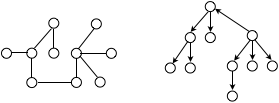
\includegraphics[scale=0.7]{FiguresGraph/tree}
       \caption{A tree with 10 vertices.}
  \label{fig:tree}
\end{center}
\end{figure}

\begin{figure}[hbt]
\begin{center}
       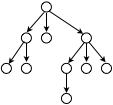
\includegraphics[scale=0.7]{FiguresGraph/outtree}
       \caption{A directed tree (out tree).}
  \label{fig:outtree}
\end{center}
\end{figure}
}

{\Denis may be it lacks a sentence here for the transition...}

A {\it directed graph} \index{graphs!directed} ({\it digraph},
\index{digraph} for short) $\g$ is given by a set of {\it nodes}
\index{graphs!node}
\index{$\n_{\fg}$: set of nodes of graph $\g$}
$\n_{\fg}$ and a set of {\it arcs}
\index{graphs!digraph!arcs}
(or {\it directed edges}) $\a_{\fg}$.
In the following, we will omit the subscript if there is no ambiguity.
\index{$\a_{\fg}$: set of arcs of digraph $\g$}
Each arc of $\g$ has the form $(u \rightarrow v)$,
\index{$\rightarrow$: arc in a directed graph}
where $u, v \in \n_{\fg}$; we say that this arc goes {\em from} $u$
{\em to} $v$.  A {\it path} 
\index{graphs!path in a digraph}
\index{path in a digraph}
in the digraph $\g$ is a sequence of arcs that share adjacent
endpoints, as in the following $(n-1)$-arc path from node $u_1$ to
node $u_n$ in $\g$:
\begin{equation}
\label{eq:di-path}
(u_1 \rightarrow u_2), \ (u_2 \rightarrow u_3), \ \ldots, \ (u_{n-2}
        \rightarrow u_{n-1}), \ (u_{n-1} \rightarrow u_n)
\end{equation}
The path (\ref{eq:di-path}) is often written in the more succinct form
\[
u_1 \ \rightarrow \ u_2 \ \rightarrow \ u_3 \ \rightarrow \cdots
\rightarrow \ u_{n-2} \ \rightarrow \ u_{n-1} \ \rightarrow \ u_n
\]
The just-described path makes sense only when every node $u_i$ belongs
to $\n_{\fg}$ and every one of its arcs, $(u_i \rightarrow u_{i+1})$,
belongs to $\a_{\fg}$.  The {\it length} of path (\ref{eq:di-path}) is
the number of arcs, i.e., $n-1$.  The existence of the path means that
the {\it distance} \index{distance!in a digraph}
\index{digraph!distance} \index{graphs!distance!in a digraph} from
$u_1$ to $u_n$ in $\g$ is no greater than $n-1$.  (There may exist
shorter paths in $\g$ from $u_1$ to $u_n$.)

{\Denis Two remarks here: First the term distance is not defined...
Second, I think we should add a brief paragraph about elementary paths, 
the Konig lemma is crucial since all the path algorithms require a finite set of vertices
(I remove the replicate nodes)}

\medskip

It is sometimes useful to endow the arcs of a digraph with labels from
an alphabet $\Sigma$.  When so endowed, the path (\ref{eq:di-path})
would be written in a form such as

\smallskip

\hspace*{.35in}$\displaystyle
(u_1 \stackrel{\lambda_1}{\rightarrow} u_2), \ 
(u_2 \stackrel{\lambda_2}{\rightarrow} u_3), \ \ldots, \ 
(u_{n-2} \stackrel{\lambda_{n-2}}{\rightarrow} u_{n-1}), \ 
(u_{n-1} \stackrel{\lambda_{n-1}}{\rightarrow} u_n)$

\smallskip

\noindent
where the $\lambda_i$ denote symbols from $\Sigma$.  Labeled paths
also are often written in a succinct manner, as:

\smallskip

\hspace*{.35in}$\displaystyle 
u_1 \ \stackrel{\lambda_1}{\rightarrow} \ u_2
    \ \stackrel{\lambda_2}{\rightarrow} \ u_3
    \ \stackrel{\lambda_3}{\rightarrow} \ \cdots \ 
    \ \stackrel{\lambda_{n-3}}{\rightarrow} \ u_{n-2}
    \ \stackrel{\lambda_{n-2}}{\rightarrow} \ u_{n-1}
    \  \stackrel{\lambda_{n-1}}{\rightarrow} \ u_n$

\medskip

If $u_1 = u_n$, then we call path (\ref{eq:di-path}) a {\em (directed)
  cycle},\index{cycle (in a digraph)} and we call its labeled version
a {\em labeled (directed) cycle}.  (The qualifier ``directed'' is
usually included only for emphasis.)

\medskip

{\Denis in the following, we move to undirected paths and intentionnally 
you changed the notation from G to H... It is interesting, but not natural for me,
I am using spontaneously the same symbol...}

An {\em undirected graph} $\h$ is given by a set of nodes $\n_{\fh}$
and a set $\e_{\fh}$ 
\index{$\e_{\fh}$: the set of edges of the undirected  graph $\h$}
of $2$-element subsets of $\n_{\fh}$.  Each of these subsets is called
an {\it edge (of $\h$)}.
\index{graphs!edge} \index{edge (in a graph)}
One can, thus, view the undirected graph $\h$ as being obtained from a
directed graph $\bar{\h}$ by removing the directionality of
$\bar{\h}$'s arcs.  Whereas we say: \\
\hspace*{.35in}the {\em arc} $(u,v)$ goes {\em from} node $u$ {\em to}
node $v$ \\
we say: \\
\hspace*{.35in}the undirected edge $\{u,v\}$ goes {\em between} nodes
$u$ and $v$ \\
or, more simply: \\
\hspace*{.35in}the undirected edge $\{u,v\}$ {\em connects} nodes $u$
and $v$.  \\
One can view an undirected graph as asserting ``pure'' connectivity,
whereas directed graphs assert some form of priority or directionality.

A {\it path} in an undirected graph \index{graphs!path in undirected
  graph} \index{path in an undirected graph} is a sequence of
edges---i.e., of $2$-element sets of nodes---such that adjacent edges
share a node.  For illustration, an $(n-1)$-edge path that connects
nodes $u_1$ and $u_n$ in the undirected graph $\h$ has the form
\begin{equation}
\label{eq:undi-path}
\{u_1, u_2\}, \ \{u_2, u_3\}, \ \ldots, \ \{u_{n-2}, u_{n-1}\}, \ \{u_{n-1}, u_{n}\}
\end{equation}
The path described in (\ref{eq:undi-path}) makes sense only when every
node $u_i$ belongs to $\n_{\fh}$ and every edge $\{u_i \ u_j\}$ belongs
to $\e_{\fh}$.  The {\it length} of path (\ref{eq:undi-path}) is the
number of edges---which is $n-1$ here; and the existence of
the path means that the {\it distance} \index{graphs!distance} 
\index{distance!in an undirected graph}
{\it between} $u_1$ and $u_n$ in $\h$ is no greater than $n-1$.  (There
may exist shorter paths that connect $u$ and $v$.)

\medskip

For each edge $\{u,v\} \in \e_{\fh}$, we call nodes $u$ and $v$ {\it
  neighbors} (in $\h$).
\index{graphs!nodes!neighbor nodes}
\index{neighbor node!in a graph}
The {\it degree}
\index{graphs!nodes!degree of a node in an undirected graph}
\index{graphs!degree of a node in an undirected graph}
\index{degree of a node in an undirected graph}
of a node $u \in \n_{\fh}$ is the number of neighbors that $u$ has.

Even at this early moment in our study of graphs, we can observe a few
important facts that can be useful when analyzing a broad range of
computation-related issues involving graphs (either as auxiliary
notions or as subjects of discourse).

\begin{prop}
\label{thm:number-edges/arcs}
{\bf (a)}
An $n$-node digraph $\g$ has no more than $n^2$ arcs.

{\bf (b)}
An $n$-node graph $\h$ has no more than $\displaystyle {n \choose 2}$ edges.

\end{prop}

\begin{proof}
{\bf (a)}
The set $\a_{\fg}$ of arcs of $\g$ is a subset of the set of ordered
pairs of nodes of $\g$.  This latter number is clearly $n^2$, because
one can choose the first node in a pair in $n$ ways and then {\em
  independently} choose the second node in $n$ ways.

\smallskip

\noindent {\bf (b)}
The stated number is the number of $2$-node subsets of $\n_{\fh}$.  To
wit, start by listing the $n^2$ ordered pairs of nodes of $\h$.
First, eliminate from the list all $n$ pairs whose first and second
elements are equal: a set of the form $\{ u,u\}$ has only one element,
hence is not an edge of $\h$.  Then, for each distinct pair of nodes
$u, v \in \n_{\fh}$, eliminate one of the two ordered pairs, $\langle
u,v \rangle$ and $\langle u,v \rangle$: both of these ordered pairs
lead to the same unordered set $\{ u,v\}$, hence the same edge of
$\h$.  After these eliminations, we are left with
\[ \frac{n^2 - n}{2} \ = \ {n \choose 2} \]
$2$-element subsets of $\n_{\fh}$, from which we choose the edges of
$\h$. \qed
\end{proof}


\begin{prop}
\label{thm:even-num-odd-degrees}
In any undirected graph, the number of nodes of odd degree is even.
\end{prop}

\begin{proof}
The result follows directly from the following equation that holds for
any undirected graph $\g$:

{\Denis we are dealing with undirected graphs and the notation is still $\g$ and not $\h$...
This is connected with my previous remark. Let take $\g$ everywhere?}
\[ \sum_{v \in {\cal N}_{\cal G}} \ \mbox{\sc degree}(v) \ = \ 2 \cdot
|\e_{\cal G}|.
\]
The equation holds because each edge $e$ of $\g$ ``touches'' two nodes
of $\g$, namely, $\e$'s two endpoints.  Since the sum of $\g$'s
node-degrees is even, each odd node-degree must be paired (in the sum)
with another odd node-degree.  \qed
\end{proof}

\medskip

We sometimes use the term {\it neighbor} within the context of {\em
  directed} graphs also.  If we say that nodes $u$ and $v$ are
neighbors in the directed graph $\g$,
\index{neighbor node!in a directed graph}
then we mean that $\a_{\fg}$ contains at least one of the arcs $(u
  \rightarrow v)$ or $(v \rightarrow u)$.  More typically, we use
  terminology that is more faithful to digraph $\g$'s directedness.
If $\a_{\fg}$ contains the arc $(u \rightarrow v)$, then we would call
  $v$ a {\it (direct) successor} of $u$
\index{digraph!successor node}
\index{successor node in a directed graph}
and we would call $u$ a {\it (direct) predecessor} of $v$
\index{digraph!predecessor node}
\index{predecessor node in a directed graph}
The term {\it parent} often replaces ``predecessor node'', and the
term {\it child} often replaces ``successor node'', especially when
$\g$ is a directed {\em tree}.  Acknowledging the distinction between
predecessors and successors in digraphs, we usually split the notion
of the degree of a node within a digraph into the {\it indegree} and
the {\it outdegree} of node $u$:
\begin{itemize}
\item
The {\it indegree} of node $u \in \n_{\fg}$
\index{digraph!indegree}
is the number of nodes $v \in \n_{\fg}$ such that $(u \rightarrow v)$
is an arc of $\g$.
\item
Symmetrically, the {\it outdegree} of node $u \in \n_{\fg}$
\index{digraph!outdegree}
is the number of nodes $v \in \n_{\fg}$ such that $(v \rightarrow u)$
is an arc of $\g$.
\end{itemize}

\smallskip

The reader will note that we nowhere guarantee that there is always a
path that connects each node $u$ with each other node $v$.  We say
that a graph $\g$ is {\it connected} \index{graphs!connected} if every
pair of nodes $u, v \in \n_{\fg}$ is connected by a path in $\g$.  If
graph $\g$ is {\em not} connected, then it is the disjoint union of
some number $c$ of connected subgraphs, usually called $\g$'s {\it
  (connected) components}.  \index{graphs!connected components} Of
course, $\g$ is connected just when $c=1$; i.e., there is a single
connected component.

\subsubsection{Graphs as a modeling tool: the {\sf 2SAT} problem}
\label{sec:graph-model-2SAT}

Now that we have the basic notions relating to connectivity in graphs,
we can develop the proof of Proposition~\ref{thm:2SAT}.  For the
reader's convenience, we restate the Proposition here.

\begin{prop}{Restatement of Proposition~\ref{thm:2SAT}}
\label{thm:2SAT-reprise}
The {\sf 2SAT} problem can be solved in polynomial time.

\noindent
That is, given any instance $\Phi$ of {\sf 2SAT}, one can determine in
time polynomial in the number of literals in $\Phi$ whether there
exists a satisfying assignment of truth-values to the variables of
$\Phi$.
\end{prop}

We develop the proof of Proposition~\ref{thm:2SAT-reprise} by focusing
on an instance of the {\sf 2SAT} problem: the following POS expression
for a propositional formula $\Phi$:
\begin{eqnarray}
\label{eq:Phi-2SAT}
\Phi & = & C_1 \ \wedge \ C_2 \ \wedge \cdots \wedge \ C_m \\
\nonumber
  & \mbox{where:} & \bullet \ \ \mbox{each clause }
 \ C_i \ = \ \ell_{i,1} \vee \ell_{i,2} \\
\nonumber
  &               & \bullet \ \ \Phi \ \ \mbox{ has $n$ logical variables}
\end{eqnarray}
We transform $\Phi$ into a directed graph $\g(\Phi)$ that has $2n$
vertices and $2n$ arcs.
\begin{itemize}
\item
For each logical variable, $x$: there is one vertex that represents
the {\em true} literal form, $x$, of variable $x$, and a second vertex
that represents the {\em false} literal form, $\bar{x}$, of the
variable.
\item
Each clause $C_i = (\ell_{i,1} \vee \ell_{i,2})$ is represented by a
pair of arcs.  Say that literal $\ell_{i,1}$ comes from variable
$x_1$, and literal $\ell_{i,2}$ comes from variable $x_2$.  These arcs
represent ``instructions'' for assigning truth-values in a way that
maximize the number of clauses that receive the value {\sc true}.
  \begin{itemize}
  \item
There is an arc $(\bar{x_1} \rightarrow x_2)$.

This arc indicates that, if variable $x_1$ is assigned truth-value
{\sc false}, then variable $x_2$ should be assigned truth-value {\sc
  true}.
  \item
Symmetrically, there is an arc $(\bar{x_2} \rightarrow x_1)$.

This arc indicates that, if variable $x_2$ is assigned truth-value
{\sc false}, then variable $x_1$ should be assigned truth-value {\sc
  true}.
  \end{itemize}
\end{itemize}
All paths in $\g(\Phi)$ represent logical implications. 

The core of our proof is the following result.

\begin{prop}
\label{prop:2SAT}
The POS formula $\Phi \ = \ C_1 \ \wedge \ C_2 \ \wedge \cdots \wedge
\ C_m$ is satisfiable if, and only if, no strongly connected component
of $\g(\Phi)$ contains both the positive form ($x$) and the negated
form ($\bar{x}$) of any variable $x$ of $\Phi$.
\end{prop}

The proof is a consequence of the two following elementary results.

\begin{lemma}
\label{lem:2SATlemma1}
If $\g(\Phi)$ contains a path from vertex $x$ to vertex $y$, then it
contains a path from vertex $\bar{y}$ to vertex $\bar{x}$.
\end{lemma}

The proof, by induction on the length of the shortest path from vertex
$x$ to vertex $y$, is left to the reader. 

\begin{lemma}
\label{lem:2SATlemma2}
If $\g(\Phi)$ contains a path from vertex $x$ to vertex $y$, then for
every truth assignment $t$ that satisfies formula $\Phi$ (i.e.,
evaluates $\Phi$ to {\sc true}), if $t$ assigns variable $x$ the
truth-value {\sc true}, then $t$ also assigns variable $y$ the
truth-value {\sc true}.
\end{lemma}

\begin{proof}
Assume that $\Phi$ is satisfied by a truth assignment $t$ which
assigns variable $x$ the truth-value {\sc true}.  Say, for
contradiction, that along the path from $x$ to $\bar{x}$ in
$\g(\Phi)$, there exists an arc (say $(\alpha \rightarrow\beta)$) such
that assignment $t$ assigns the value {\sc true} to $\alpha$ and the
value {\sc false} to $\beta$.  Because of the way we constructed
$\g(\Phi)$, the existence of this arc means that $\Phi$ contains the
clause $\bar{\alpha} \vee \beta$.  Moreover, under truth assignment
$t$, this clause of $\Phi$ evaluates to {\sc false}, because both of
its literals are assigned value {\sc false}.  This contradicts the
assumption that $t$ is a satisfying assignment for $\Phi$.  \qed
\end{proof}

We finally prove the main result of this section,
Proposition~\ref{prop:2SAT}.

\begin{proof}[Proposition~\ref{prop:2SAT}]
Focus on a POS formula $\Phi$ and its associated digraph $\g(\Phi)$.

{\bf Necessity}.
Say first that $\g(\Phi)$ has a strongly connected component which
contains vertices arising from a variable $x$ in both positive ($x$)
and negated ($\bar{x}$) forms.  We claim that $\Phi$ is not
satisfiable.

Now, by definition of ``strongly connected'', $\g(\Phi)$ must contain
paths between the vertices corresponding to $x$ and $\bar{x}$.  By
Lemma~\ref{lem:2SATlemma2}, therefore, any truth-assignment that could
satisfy formula $\Phi$ would have to assign literals $x$ and $\bar{x}$
the same truth-value.  Any such truth-assignment to formula $\Phi$'s
{\em literals} would not be a valid truth-assignment to $\Phi$'s {\em
  variables} (specifically to variable $x$).  We conclude that no
valid truth-assignment could satisfy formula $\Phi$.

\medskip

{\bf Sufficiency}.
Say next that $\g(\Phi)$ has no strongly connected component which
contains vertices arising from a variable $x$ in both positive ($x$)
and negated ($\bar{x}$) forms.  We construct a truth-assignment $t$ to
$\Phi$'s variables under which $\Phi$ evaluates to {\sc true}.
Assignment $t$ witnesses $\Phi$'s satisfiability.

We construct a satisfying truth-assignment $t$ for $\Phi$ as follows.

\noindent {\bf 1.}
Say that graph $\g(\Phi)$ has $k$ mutually disjoint strongly connected
components.  We label these components in {\it topological order},
\index{topological order} as $S_1, S_2, \ldots, S_k$.  The phrase
{\it ``topological order''} means the following.
\begin{itemize}
\item
$\g(\Phi)$ contains no arc of the form $(u \rightarrow v)$ where
  vertex $u$ belongs to some component $S_i$, and vertex $v$ belongs
  to some component $S_j$ with $j < i$.
\end{itemize}
We know that this labeling is possible because any such arc would make
all vertices of $S_j$ accessible from all vertices of $S_i$, and
conversely.  This would mean that $S_i$ and $S_j$ would be contained
within the same strongly connected component---which would contradict
their assumed disjointness.

\medskip

\noindent {\bf 2.}
We assign truth-values to variables of $\Phi$ by scanning the
vertices/literals of $\g(\Phi)$ in decreasing order of the topological
indices of $\g(\Phi)$'s strongly connected components.
\begin{itemize}
\item
The {\em first time} that we encounter a vertex/literal $\ell$, in
true or negated form, we assign the truth-value to $\ell$'s associated
variable that makes literal $\ell$ {\sc true}.  This strategy also
makes the clause that this instance of literal $\ell$ occurs in
evaluate to {\sc true}.
\item
If we encounter an instance of a vertex/literal $\ell$ whose
associated variable has already been assigned a truth-value, then we
assign to this instance a truth-value that is consistent with the
variable's assignment: a positive literal gets the same assignment,
while a negative instance gets the negated version of the assignment.
\end{itemize}

Proceedings in this fashion, we develop a truth-assignment that
satisfies all of $\Phi$'s clauses.  To wit, assume for contradiction
that some clause of $\Phi$, say $(\xi \vee \eta)$, is not satisfied
under our procedure.  This means, in particular, that our assignment
$t$ assigns the truth-value {\sc false} to vertex/literal $\xi$.  But,
this can happen only if $t$ has assigned the truth-value {\sc true} to
vertex/literal $\bar{\xi}$, within a strongly connected component of
$\g(\Phi)$ whose index is higher than that of the strongly connected
component that $\xi$ occurs in.  The same observation applies to
vertex/literal $\eta$.  But this is impossible, because within our
construction of $\g(\Phi)$, the clause $(\xi \vee \eta)$ in formula
$\Phi$ would add the arc $(\bar{\xi} \rightarrow \eta)$ to graph
$\g(\Phi)$.  It fallows that we have found a truth assignment that
satisfies formula $\Phi$, as was claimed.  \qed
\end{proof}

\medskip

We close with two small examples to illustrate
Proposition~\ref{prop:2SAT}
\begin{enumerate}
\item
Fig.~\ref{2SATyes} illustrates $\g(\Phi_1)$, for the formula
\[ \Phi_1 \ = \ (\bar{x}_{3} \vee \bar{x}_{1}) \ \wedge \
 (x_{1} \vee \bar{x}_{2}) \ \wedge \ (x_{2} \vee x_{3})
\]
The graph has the two strongly connected components illustrated in the
figure.  One can thereby read off the following satisfying truth-value
assignment $t$ for formula $\Phi_1$: $t(x_1) = \mbox{\sc false}$;
$t(x_2) = \mbox{\sc false}$; $t(x_3) = \mbox{\sc true}$.
\begin{figure}[h]
\begin{center}
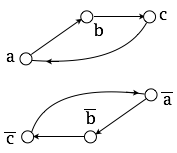
\includegraphics[width=0.3\textwidth]{FiguresGraph/2SATyes.png}
\caption{A portion of the digraph $\g(\Phi_1)$.  The graph's two
  strong components provide a truth assignment for $\Phi_1$: $t(x_1) =
  \mbox{\sc false}$; $t(x_2) = \mbox{\sc false}$; $t(x_3) = \mbox{\sc
    true}$.}
\label{2SATyes}
\end{center}
\end{figure}

\item
Fig.~\ref{2SATno} illustrates $\g(\Phi_2)$, for the formula
\[ \Phi_2 \ = \ (\bar{x}_{3} \vee \bar{x}_{1}) \ \wedge \                                      
(\bar{x}_{1} \vee x_{3}) \ \wedge \ (x_{2} \vee x_{3})
\]
Because the graph contains a (directed) path from vertex $x_1$ to
vertex $\bar{x}_1$, Proposition~\ref{prop:2SAT} assures us that formula
$\Phi_2$ does not admit any satisfying truth-assignment.
\begin{figure}[h]
\begin{center}
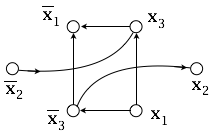
\includegraphics[width=0.3\textwidth]{FiguresGraph/2SATno.png}
\caption{A portion of the digraph $\g(\Phi_2)$.  Because the graph
  contains  a path from vertex $x_1$ to vertex $\bar{x}_1$,  formula
  $\Phi_2$ does not admit any satisfying truth-assignment.}
\label{2SATno}
\end{center}
\end{figure}
\end{enumerate}

\medskip

Even without formal background in algorithmics, it is clear that the
processes of: constructing digraph $\g(\Phi)$ from formula $\Phi$;
isolating and investigating the strongly connected components of
$\g(\Phi)$ can be accomplished in a number of computational steps that
is polynomial in thesize of $\Phi$.  This validates
Proposition~\ref{prop:2SAT}.  \qed



\subsubsection{Distance-related concepts}

\noindent {\it Distance and diameter in a digraph.}
\index{digraph!distance between two nodes}
Extrapolating from our discussion of path (\ref{eq:di-path}): The {\it
  distance} from node $u_1$ to node $u_n$ in the digraph $\g$ is the
smallest number of arcs in any path from $u_1$ to $u_n$.  In detail:
\begin{equation}
\label{eq:di-distance-defn}
 \mbox{\sc distance}(u_1, u_n) \ \ \left\{
\begin{array}{cll}
= & 0 & \mbox{  if  } \ u_1 = u_n \\
\leq & n-1 & \mbox{  if there is a path } \ (\ref{eq:di-path})
\ \mbox{ from $u_1$ to $u_n$} \\
= & \infty & \mbox{  if there is no path } \ (\ref{eq:di-path})
\ \mbox{ from $u_1$ to $u_n$}
\end{array}
\right.
\end{equation}
The {\it diameter} \index{diameter in a digraph}
\index{digraph!diameter} of a directed graph $\g$ is the largest
distance between two nodes of $\g$, i.e., the largest number $d$ for
which there exist nodes $u_1, u_n \in \n_{\fg}$ such that {\sc
  distance}$(u_1, u_n) = d$.  Note that when discussing digraphs, we
always use {\em directed} paths when defining distance.

\medskip

\noindent {\it Distance and diameter in an undirected graph.}
\index{graphs!!distance between two nodes}
\index{diameter in a graph}
Extrapolating from our discussion of path (\ref{eq:undi-path}): The
{\it distance between} node $u_1$ and node $u_n$ in the graph $\g$ is
the smallest number of edges in any path from $u_1$ to $u_n$.  In
detail:
\begin{equation}
\label{eq:distance-defn}
 \mbox{\sc distance}(u, v) \ \ \left\{
\begin{array}{cll}
= & 0 & \mbox{  if  } \ u = v \\
\leq & n-1 & \mbox{  if there is a path } \ (\ref{eq:di-path})
\ \mbox{ between $u$ and $v$} \\
= & \infty & \mbox{  if there is no path } \ (\ref{eq:di-path})
\ \mbox{ between $u$ and $v$}
\end{array}
\right.
\end{equation}
{\Denis Same remark as before, we are dealing with undirected graphs and the notation is $\g$ instead of $\h$...}

The {\it diameter} \index{diameter in a graph} \index{graphs!diameter}
of an undirected graph $\h$ is the largest distance between two nodes
of $\h$, i.e., the largest number $d$ for which the exist nodes $u_1,
u_n \in \n_{\fh}$ such that {\sc distance}$(u_1, u_n) = d$.  Note that
when discussing undirected graphs, we always use {\em undirected}
paths when defining distance.

\ignore{********
Alternatively, this result can be proved by applying the Fubini's
principle using the adjacency matrix.  The two ways of counting the
non-zero elements are by rows (giving the sum of degrees) and globally.
\bigskip

Now, decompose this sum into even and odd degrees.

$\Sigma_{x \in V} \delta(x) = \Sigma_{x \in V_{even}} \delta(x) +
\Sigma_{x \in V_{odd}} \delta(x)$.

As $\Sigma_{x \in V_{even}} \delta(x)$ is obviously even as the sum of
even numbers, $\Sigma_{x \in V_{odd}} \delta(x)$ should also be even.

Thus, the number of odd vertices is even.% as depicted in Figure~\ref{propertyOdd}.
*************}

\bigskip
\noindent \fbox{
\begin{minipage}{0.95\textwidth}
Our discussion of internode distances within graphs have focused on
shortest (or longest) path problems in {\em unweighted} graphs.  A
variety of important applications can be modeled via path-distance
problems in graphs $\g$ each of whose edges, say, $\{u,v\}$, is
weighted with a number that measures the cost of going between nodes
$u$ and $v$ in $\g$.  Of course, when graph $\g$ is directed, then the
arcs $(u \rightarrow v)$ and $(v \rightarrow u)$ can have different
weights, to model situations wherein going from $u$ to $v$ is
easier/cheaper than going from $v$ to $u$.  Happily, determining
shortest (or longest) paths in a directed or undirected graph $\g$ can
be accomplished ``efficiently''---which in the algorithmic world means
``in a number of steps that is polynomial in the size of $\g$''.
 \end{minipage}
}

%%%%%%%%%%%%%%%%%%%%%%%%%%%%%%%%%%%%

\subsubsection{Matchings in graphs}
\index{graphs!matching}

The notion of a {\it matching} in a graph is fundamental to many
situations that can be modeled using graphs.  A {\it matching} in an
undirected graph $\g$ is a set of edges of $\g$ that have no nodes in
common.  It is, thus, a formal mechanism for pairing nodes of a graph.
The broad array of activities that can be modeled using graph matching
include: pairing competitors for a tennis tournament; helping a person
select a potential spouse (which even in the vernacular is often
termed ``matchmaking''); determining (near-)optimal layouts for a
keyboard in language X (based on the relative ``affinities'' of
various pars of letters for one another in language X); selecting
persons to command the police stations in city Y (based on the
perceived ``match'' between a candidate's qualifications and the needs
of specific stations).  Even this small sampler of situations that
involve matchings makes it clear that there are many variations on
this formal theme.  This section is devoted to describing, and briefly
discussing, a few of the most commonly encountered versions of
matching in graphs.
\bigskip

\noindent \fbox{
\begin{minipage}{0.95\textwidth}
Although the definitions of the various versions of matching are
readily accessible to even the beginning student of mathematics, much
of the more sophisticated mathematical knowledge about matchings is
beyond any beginning text.  The interested reader might consult a more
advanced source, such as \cite{Berge73}, to get a feeling for what is
known about this simple, yet rich, topic.
\end{minipage}
}
\bigskip

\noindent {\it Matchings in unweighted graphs}.
The most straightforward notion of matching involves an undirected
graph $\g$ with unlabeled edges.  The optimization criterion most
often invoked with this genre of matching is to maximize the number of
edges of $\g$ that belong to the matching.

The target in this ``vanilla-flavored'' matching problem is often a
matching that is {\em maximal}, \index{graphs!maximal matching}
\index{graphs!maximal matching!unweighted graph} in the sense that
adding any further edge of $\g$ to the matching leaves one with a set
of edges that is no longer a matching.

Among maximal matchings in a graph $\g$, the ``ultimate treasure'' is
a matching that is {\it perfect}, \index{graphs!perfect matching} in
the sense that every node of $\g$ belongs to some edge of the
matching.

\begin{prop}
\label{thm:max-matching}
Maximal matchings exist for any graph $\g$.  One can find such a
matching in a number of steps proportional to $|\n_{\fg}|$.
\end{prop}

\begin{proof}
We leave to the reader the challenge of verifying that the following
\index{greedy algorithm} {\em greedy}\footnote{In the world of
  algorithmics, the term ``greedy'' describes any process that seeks to
  satisfy a criterion as quickly as possible, with no consideration of
  how this choice affects future choices.}~process satisfies the
conditions of the Proposition.

{\Denis Rewrite with the algo style and put it in a more algorithmic language}
\noindent
{\it The Process:} \\
Begin by laying the nodes of $\g$ out, left to right, in any way.
Repeat the following process until no nodes remain in the layout.

\noindent
Select the leftmost node, $u$, in the remaining layout of $\n_{\fg}$.
Select the leftmost neighbor, $v$, of $u$ that remains in the layout.
  \begin{enumerate}
  \item
If you succeed in finding both $u$ and $v$, then add edge $\{u,v\}$ to
the matching we are building.  Remove both $u$ and $v$ from the
layout.
  \item
If there is no neighbor $v$ of $u$ in the remaining layout, then
remove node $u$ from the layout.
  \end{enumerate}
The real challenge here is to find a data structure that allows an
efficient search for a ``remaining'' neighbor-node $v$ at each step of
the selection process.
\qed
\end{proof}

\medskip

In contrast to maximal matchings, there exist myriad simple graphs
that do not admit any perfect matching.  Contemplating, for instance,
matchings within any cycle with an odd number of nodes may prepare the
reader for the challenge of verifying the following necessary
condition for a graph to admit a perfect matching.

\begin{prop}
\label{thm:necessary-for-perfect-matching}
Let $\g$ be a graph that admits a perfect matching.  Then:
\begin{itemize}
\item
$\g$ has an even number of nodes.
\item
The cardinality of the (perfect) matching---i.e., the number of edges
in the matching---is exactly
$\frac{1}{2}|\n_{\fg}|$.
\end{itemize}
\end{prop}


\bigskip

\noindent {\it Matchings in weighted graphs}.
The other very popular genre of matching problem focuses on graphs
each of whose edges, say, $\{u,v\}$, is weighted with a number that
measure the ``affinity'' of  nodes $u$ and $v$ for each other.  The
challenge is to find a matching that is {\em maximal}
\index{graphs!maximal matching} in the sense of having a cumulative
sum of edge-weights that is not exceeded by any other matching's.

We note in closing that, while edge-weightings often complicate
computational processing of graphs, they need not render such
computations practically infeasible.  For instance, the problem of
discovering a perfect matching of minimal weight in an edge-weighted
graph can be solved moderately efficiently---i.e., in a number of
steps that is polynomial in the size of the graph.  (An algorithm that
achieves this efficiency can be based on the colorfully named {\it
  Hungarian assignment method}; \index{Kuhn, Harold W.}  see the
original source \cite{Kuhn55} or the encyclopedic algorithms text
\cite{CLRS}.)










%%%%%%%%%%%%%%%%%%%%%%%%%%%%%%%%%

\subsection{Trees}
\label{sec:Trees}

The special class of graphs called {\it trees} \index{graphs!trees}
\index{trees} occupy a place of honor within both the mathematical
field called {\it graph theory} and within the vernacular.
They are identified mathematically as graphs that contain no
cycles or, equivalently, as graphs in which each pair of nodes is
connected by a unique path: a tree is thus the embodiment of ``pure''
connectivity (see Fig.~\ref{fig:tree} for an example of tree).  As one
would expect from the vernacular, a set of trees is called a {\it
  forest}. \index{forest (of trees)}
\begin{figure}[hbt]
\begin{center}
       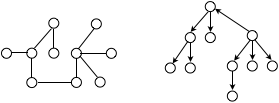
\includegraphics[scale=0.7]{FiguresGraph/tree}
       \hspace{1cm}
       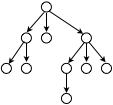
\includegraphics[scale=0.7]{FiguresGraph/outtree}
       \caption{An undirected tree with 10 vertices (left) and a directed out tree (right).}
  \label{fig:tree}
\end{center}
\end{figure}


Mathematically speaking, a tree is a graph that contains no cycles,
i.e., is {\it cycle-free}. \index{graphs!cycle-free} Equivalently, a
tree is a graph in which each pair of distinct nodes is connected by
precisely one path.  A tree is thus the embodiment of ``pure''
connectivity: it provides the minimal interconnection structure that
provides paths that connect every pair of nodes.  As one might expect
from the vernacular, a set of trees is called a {\it forest}. \index{forest (of trees)}

We have just given two distinct definitions of ``tree''.  The reader
should prove that both definitions define the same class of graphs.

\begin{prop}
\label{thm:2defns-trees}
Prove that the two definitions of ``tree'' are equivalent.  In other
words, prove that the following assertions about a connected graph
$\t$ are equivalent, in the sense that one assertion holds if, and
only if, the other does.
\begin{enumerate}
\item
The graph $\t$ is cycle-free.
\item
Each pair of distinct nodes of $\t$ is connected by precisely one
path.
\item
An $n$-node connected tree $\t$ has precisely $n-1$ edges.
\end{enumerate}
\end{prop}

Let us detail the proof of the last property.

\begin{proof}
\noindent 
Let us proceed by induction on $n$.

The base case $n=2$ is obvious, because one edge is both necessary and
sufficient to connect two nodes.

Assume for induction that the indicated tally is correct for all trees
having no more than $k$ nodes.

Consider, for the purpose of extending the induction, any tree $\t$ on
$k+1$ nodes.  Easily, $\t$ must contain at least one leaf-node---i.e.,
a node $v$ of degree $1$---or else $\t$ would contain a cycle.  If we
remove $v$ and its incident edge, we now have a tree on $k$ nodes
which, by induction, has $k-1$ edges.  When we reattach node $v$, to
restore $\t$ to its original state, we see that $\t$ has $k+1$ nodes
and $k$ edges.

Because $\t$ was an arbitrary $(k+1)$-node tree, the induction is
extended.  \qed
\end{proof}

\bigskip

\noindent \fbox{
\begin{minipage}{0.95\textwidth}
Sociologically, the historical {\it atomic family tree} \index{family
  tree} has two roots, representing the matriarch and patriarch of the
family.  The entirety of the tree represents a single family
generationally, before any children form their own families.  All
child-nodes in this genre of tree are the roots of singly-rooted
subtrees of the entire family tree.  The leaves of the tree are the
childless descendants of the roots.  Note that, while we are using
anthropomorphic language here, we could be discussing other genres of
``family'', as, e.g., many types of biological taxonomies.
\end{minipage}
}
\bigskip

Among rooted directed trees, an important subclass comprises those
that have a {\em single root} which has a directed path to every other
node.  The length of each such directed path is often used to label
the {\it generation}
\index{generation of a node in a singly-rooted directed tree}
of the node at the end of the path: root, child, grandchild,
great-grandchild, etc.
Every node of the tree is the root of a singly-rooted directed
subtree of the entire tree.  All subtrees that are rooted at nodes of
the same generation are mutually disjoint.
\bigskip

\noindent \fbox{
\begin{minipage}{0.95\textwidth}
A singly-rooted tree represents a {\it hierarchy}.
\index{trees!singly-rooted!hierarchy} \index{hierarchy} Given two
directed subtrees within a hierarchy, either the root of one of the
subtrees is a descendant of the root of the other, or the two subtrees
are are mutually disjoint.
\end{minipage}
}
\bigskip

More formally: {\em rooted trees} are a class of {\em acyclic}
digraphs.  Paths in trees which start at the root are often called
{\em branches}.  The {\em acyclicity} of a tree $\t$ means that for
any branch of $\t$ of the form (\ref{eq:di-path}), we cannot have $u_1
= u_n$, for this would create a cycle.  Each singly-rooted tree $\t$
has a designated {\em root node} \index{trees!root node} $u_n \in
\n_{\ft}$ that resides at the end of a branch (\ref{eq:di-path}) that
starts at $r_{\ft}$ (so $u_1 = r_{\ft}$) is said to reside at {\em
  depth} $n-1$ in $\t$; by convention, $r_{\ft}$ is said to reside at
depth $0$.  \index{depth of a node in a singly-rooted trees} $\t$'s
root $r_{\ft}$ has some number (possibly $0$) of arcs that go from
$r_{\ft}$ to its {\em children,} each of which thus resides at depth
$1$ in $\t$; in turn, each child has some number of arcs (possibly
$0$) to its children, and so on.  For each arc $(u \rightarrow v) \in
A_{\ft}$, we call $u$ a {\it parent} \index{trees!parent node} of $v$,
and $v$ a {\it child} \index{trees!child node} of $u$, in $\t$;
clearly, the depth of each child is one greater than the depth of its
parent.  Every node of $\t$ except for $r_{\ft}$ has precisely one
parent; $r_{\ft}$ has no parents.  A childless node of a tree is a
{\em leaf}, \index{trees!leaf node} i.e., a node of degree $1$.  The
transitive extensions of the parent and child relations are,
respectively, the {\em ancestor} \index{trees!ancestor node} and {\em
  descendant} \index{trees!descendant node} relations.  The {\em
  degree} \index{degree (of a node in a tree)} of a node $v$ in a tree
is the number of children that the node has, call it $c_v$.  If every
non-leaf node in a tree has the same degree $c$, then we call $c$ the
{\em degree of the tree}.  \index{degree of a tree}

It is sometimes useful to have a symbolic notation for the ancestor
and descendant relations.  To this end, we write $(u \Rightarrow v)$
\index{$\Rightarrow$: ancestor/descendant in a rooted tree} to
indicate that node $u$ is an {\it ancestor} of node $v$, or
equivalently, that node $v$ is a {\it descendant} of node $u$.  If we
decide that we are not interested in {\em really distant} descendants
of the root of a tree $\t$, then we can {\em truncate} \index{truncated}
$\t$ at a desired depth $d$ by removing all nodes whose depths exceed
$d$.  We thereby obtain the {\em depth-$d$ prefix} of $\t$.

\ignore{****************
Figure \ref{fig.graph-samples} depicts an arc-labeled rooted tree $\t$
whose arc labels come from the alphabet $\{a,b\}$.  $\t$'s arc-induced
relationships are listed in Table~\ref{tab.graph-samples}.
\begin{figure}[htb]
\centerline{\epsfig{figure=graph.sample.eps,height=4truecm}}
\caption{An arc-labeled rooted tree $\t$ whose arc labels come from
  the alphabet $\{a,b\}$.  (Arc labels have no meaning; they are just
  for illustration.)
\label{fig.graph-samples}}
\end{figure}
\begin{table}[htb]
{\small
\begin{center}
\fbox{
\begin{tabular}{c||c|c|c|c}
\multicolumn{5}{c}{The arc-labeled rooted tree $\t$ of
  Figure \ref{fig.graph-samples}} \\
\hline
Node            & Children & Parent & Descendants & Ancestors \\
\hline
\hline
$r_{\ft} = u_0$ 
& $u_1$
& none & 
$u_1, u_2, \ldots, u_k, v_1, v_2, \ldots, v_k,
w_1, w_2, \ldots, w_k$
& none \\
\hline
$u_1$
& $u_2, v_1$
& $u_0$ & 
$u_2, \ldots, u_k, v_1, v_2, \ldots, v_k, w_1, w_2, \ldots, w_k$
& $u_0$ \\
\hline
$u_2$
& $u_3, v_2$
& $u_1$ & 
$u_3, \ldots, u_k, v_2, \ldots, v_k, w_2, \ldots, w_k$
& $u_0$ \\
\hline
 $\vdots$ & $\vdots$ & $\vdots$ &  $\vdots$ &  $\vdots$ \\
\hline
$u_k$
& $v_k$ 
& $u_{k-1}$ & 
$v_k, w_k$
& $u_0, u_1, \ldots, u_{k-1}$ \\
\hline
$v_1$
& $w_1$ 
& $u_1$ & 
$w_1$
& $u_0, u_1$ \\
\hline
$v_2$
& $w_2$
& $u_2$ & 
$w_2$
& $u_0, u_1, u_2$ \\
\hline
 $\vdots$ & $\vdots$ & $\vdots$ &  $\vdots$ &  $\vdots$ \\
\hline
$v_k$
& $w_k$
& $u_k$ & 
$w_k$
& $u_0, u_1, \ldots, u_k$ \\
\hline
$w_1$
& none
& $v_1$ & 
none
& $u_0, u_1, v_1$ \\
\hline
$w_2$
& none &
$v_2$ & 
none
& $u_0, u_1, u_2, v_2$ \\
\hline
$w_k$
& none
& $v_k$ & 
none
& $u_0, u_1, \ldots, u_k, v_k$
\end{tabular}
}
\end{center}
}
\caption{A tabular description of the rooted tree $\t$ of
  Figure \ref{fig.graph-samples}.  \label{tab.graph-samples}}
\end{table}
*********************}

\subsubsection{Spanning trees}

One of the major uses of trees and forests is as a way of succinctly
``summarizing'' the connectivity structure inherent in an undirected
graph.  This role is inherent in the notion of a {\it spanning tree}
\index{graphs!spanning tree} \index{spanning tree} of a connected
graph $\g$.  A spanning tree of $\g$ is a tree $\t(\g)$ whose node-set
is identical to $\g$'s:
\[ \n_{\ft(\fg)} \ = \ \n_{\fg} \]
and all of whose edges are edges of $\g$:
\[ \e_{\ft(\fg)} \ \subseteq \ \e_{\fg}. \]
Not surprisingly, a connected graph $\g$  typically has {\em many}
spanning trees.  All such trees share $\g$'s node-set, but they may
choose quite different sets of edges.

\ignore{
{\Arny Chance for some exercises here}

For a graph $\g$ that is not connected, we replace the notion of
spanning tree of $\g$ with the analogous notion of a {\it spanning
  forest} \index{graphs!spanning forest} \index{spanning forest} of
$\g$.  We shall typically discuss only spanning trees in this section,
leaving the reader to extrapolate the discussion to include spanning
forests of unconnected graphs.
}


The major use of spanning trees in applications is to ``summarize''
the full connectivity structure of a graph---and of the entities that
the graph models, such as a map, the layout of a museum, etc.  When
used in this way, the edges of spanning trees are typically {\em
  weighted}, \index{graphs!spanning tree!edge-weighted} in order to
model a ``cost'' of incorporating that edge in the tree.  The types of
computational problem modeled via edge-weighted spanning trees
include: the optimal placement of firehouses, or hospitals, in a town
and the optimal deployment of security mechanisms in an art museum.
Reflecting problems wherein edge-weights measure transit costs, it is
a classical computational problem to seek a {\em minimum-weight
  spanning tree} \index{graphs!minimum-weight spanning tree}
\index{minimum-weight spanning tree} (or, in the vernacular, a {\em
  minimum spanning tree}).  Happily, this classical optimization
problem can be solved within a number of steps that is linear in the
number of edges of $\g$ \cite{CLRS}.

\ignore{
I put in the exercice session
{\Arny Giving just a {\em hint} at a solution for MST to real
  beginners is probably useless}

There are mainly two ways for constructing such a MST, each one
emphasizes a different propriety of the MST, namely, avoid cycles and
minimize the span.  In both cases, the edges are sorted in increasing
order of weights.  More precisely, the first one constructs a subtree
which partially spans the graph by adding at each step the minimum
neighboring edge while the other add successively the edges of minimal
weights that do not create a cycle.
}

Just as with graphs, there is a {\em directed} version of trees which
is formed by replacing the (unoriented) edges of an undirected tree by
(oriented) arcs; see the right side of Fig.~\ref{fig:tree}.  Within a directed tree
$\t$, one often says that an arc goes from a {\it parent node}
\index{trees!parent node} to a {\it child node} \index{trees!child
  node}.  Extending this anthropomorphic metaphor, one often talks
about the {\it ancestor(s)} \index{trees!ancestor node} and {\it
  descendant(s)} \index{trees!descendant node} of a tree-node.  We
single out two special classes of nodes: A {\it root (node)}
\index{trees!root (node)} \index{root (of a directed tree)} of $\t$ is
defined by its having no entering arcs, i.e., indegree $0$; a {\it
  leaf (node)} \index{trees!leaf (node)} \index{leaf (of a directed
  tree)} of $\t$ is defined by its having no exiting arcs, i.e.,
outdegree $0$.  The reader is certainly familiar with the use of
rooted directed trees to represent family trees and corporate
hierarchies.

%%%%%%%%%%%%%%%%%%%%%%%%%%%%%%%%%%%

\subsection{Computationally Significant ``Named'' Graphs}
\label{sec:graphs-important-families}

The mathematical discipline called graph theory is an important source
of formal aids for the activities of designing, analyzing, utilizing,
and verifying computer systems.  Of course, computer systems are
designed by humans.  Among other consequences of this fact is the
observations that the graphs that are among the most commonly used to
structure systems tend to be rather uniform in structure, in a variety
of possible ways.  Such graphs, when drawn, often exhibit a lot of
structural symmetry.  One popular form of symmetry is {\it degree
  regularity}: an undirected graph $\g$ is {\it regular}
\index{graphs!regular} if all nodes of $\g$ have the same degree.  Not
surprisingly, there is a directed version of ``regular'' embodied in the
symmetric notions of {\it in-regularity}
\index{graphs!directed!in-regular} and {\it out-regularity}.
\index{graphs!directed!out-regular}

\medskip

We now describe five families of regular graphs that have proven
useful over the history of digital computing, and we expose some basic
properties of each, including its diameter.  Each of these graphs is
available in both a directed and an undirected version, although, as
we note, one of these versions is more commonly encountered.  We have
selected these specific graphs for rather different reasons.
\begin{itemize}
\item
The first two graphs, the {\it cycle-graph} of paragraph {\small\sf A}
and the {\it complete graph} of paragraph {\small\sf B} were selected
for respectively representing the lowest-degree and highest-degree
graphs that share two properties: (1) every node of each graph is
accessible from every other node; (2) all nodes ``look alike'' to
someone traversing the graph.  Elaborating on (2): If we put you down
on a node of either graph, there is no way that you can determine the
identity of that node.  This is an important feature to ponder,
because it is a simple instance of the anonymity problem inherent to
many modern distributed computing environments.  {\it How does one
  orchestrate cooperative activities when all agents ``are
  identical''?}
\item
The remaining graphs, the {\it mesh and torus networks}\footnote{These
  two structures, though distinct, are usually discussed together
  because they share so many important properties.}~of paragraph
{\small\sf C}, the {\it hypercube network} of paragraph {\small\sf D},
and the {\it de Bruijn network} of paragraph {\small\sf E}, were
selected for their importance within the world of parallel and
distributed computing---as abstract platforms for developing efficient
computational and communicational processes, and as abstract versions
of the networks that underlie parallel architectures by
interconnecting its processors.
\end{itemize}
Throughout, the parameters that describe our graph families range over
the positive integers; i.e., each occurrence of $n$ below ranges over
$\N^+$.

\subsubsection{The cycle-graph $\cc_n$}

For each positive integer $n \in \N^+$, both the {\it undirected
  order-$n$ cycle-graph} $\cc_n$ and the {\it directed order-$n$
  cycle-graph} $\widehat{\cc}_n$ \index{cycle graph} \index{cycle
  network} have {\it node-set}
\[ \n_{{\cal C}_n} \ = \ \n_{\widehat{{\cal C}}_n}
\ = \ \{ 0, \ 1, \ \ldots, \ n-1\}. \]
\begin{itemize}
\item
$\cc_n$ has $n$ edges; its {\it edge-set} is
\[ \e_{{\cal C}_n} \ = \
\big\{ \{i, \ i+1 \bmod n\} \ \ | \ \ i \in \{0, \ 1, \ \ldots,
\ n-1\} \big\}.
\]
Fig.~\ref{fig:cycle} illustrates a cycle with $8$ vertices.
  \begin{itemize}
  \item \index{cycle graph!node-degree}
$\cc_n$ is a regular network: each node has degree $2$.

Specifically, each node $i$ of $\cc_n$ has its {\it predecessor} $i-1
\bmod n$ \index{cycle graph!predecessor node} \index{cycle
  graph!successor node} and its {\it successor} $i+1 \bmod n$ .
  \item \index{cycle graph!diameter}
$\cc_n$ has diameter $\lfloor n/2 \rfloor$.

Direct calculation shows that $\cc_n$'s diameter is no larger than
this.  The fact that this is, in fact, the graphs's diameter is
witnessed by the distance between each node $k \in \n_{{\cal C}_n}$
and its antipodal node $k + \lfloor n/2 \rfloor \bmod n$.
  \end{itemize}

\item
$\widehat{\cc}_n$ has {\it arc-set}
\[ \a_{\widehat{{\cal C}}_n} \ = \ 
\big\{ (i \rightarrow i+1 \bmod n) \ \ | \ \ i \in \{0, \ 1, \ \ldots, \ n-1\} \big\}
\]
  \begin{itemize}
  \item \index{cycle graph!directed node-degree}
$\widehat{\cc}_n$ is a regular network: each node has the same
    indegree and the same outdegree.  Coincidentally, both the common
    indegree and the common outdegree are $2$.
  \item
$\widehat{\cc}_n$ has (directed) diameter $n-1$.

Of course, $n-1$ is an upper bound on the diameter of any $n$-node
digraph.  The fact that this is exactly the graph's diameter is
witnessed by the directed distance from each node $k$ of $\widehat
{\cc}_n$ to its predecessor node $k-1 \bmod n$.
  \end{itemize}
\end{itemize}

\begin{figure}[hbt]
\begin{center}
       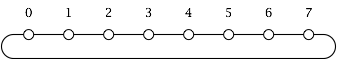
\includegraphics[scale=0.7]{FiguresGraph/cycle}
       \caption{A cycle of $8$ vertices.}
  \label{fig:cycle}
\end{center}
\end{figure}

\subsubsection{The complete graph, or, clique $\k_n$}
\label{sec:cliques}
\index{complete graph} \index{clique}

For each positive integer $n \in \N^+$, we denote by $\k_n$ the {\em
  undirected} order-$n$ {\it complete-graph} (or, {\it clique}),
\index{complete graph} \index{clique} and by $\widehat{\k}_n$ the {\em
  directed} order-$n$ {\it complete-graph} (or, {\it clique}).  Both
$\k_n$ and $\widehat{\k}_n$ have {\it node-set}
\[ \n_{{\cal K}_n} \ = \ \n_{\widehat{{\cal K}}_n}
\ = \ \{ 0, \ 1, \ \ldots, \ n-1\}. \]
\begin{itemize}
\item
$\k_n$ has $\displaystyle {n \choose 2}$ edges; its {\it edge-set} is
\[ \e_{{\cal K}_n} \ = \
\big\{ \{i, \ j\} \ \ | \ \ i,j \in \{0, \ 1, \ \ldots, \ n-1\}, \ i
\neq j \big\}.
\]
  \begin{itemize}
  \item \index{complete graph!node-degrees} \index{clique!node-degrees}
$\k_n$ is a regular network: each node has degree $n-1$; every node $i
\in \n_{\fk_n}$ is connected with all other nodes.

   \item \index{complete graph!diameter}
$\k_n$ has diameter $1$.

$\k_n$'s diameter is a direct consequence of its node-degrees, and vice versa.
  \end{itemize}

\item
$\widehat{\k}_n$ has $(n-1)n$ arcs; its {\it arc-set} is
\[ \a_{\widehat{{\cal K}}_n} \ = \ 
\big\{ (i \rightarrow j) \ \ | \ \ i,j \in \{0, \ 1, \ \ldots, \ n-1\}
\big\}, \ i \neq j
\]
  \begin{itemize}
  \item
$\widehat{\k}_n$ is a regular network: each node has the same indegree
    and the same outdegree.  Both the common indegree and the common
    outdegree are $n-1$.
  \item
$\widehat{\k}_n$ has (directed) diameter $1$.

As in the undirected case, there is a causal relationship between
$\widehat{\k}_n$'s diameter and its (in- and out-) node-degrees.
  \end{itemize}
\end{itemize}

Hearkening back to our discussion of matchings in (unweighted) graphs:
The structure of the set of perfect matchings in general graphs is
decidely nontrivial.  For clique-graphs, though, the structure is much
easier to discuss.

\begin{prop}
\label{thm:perfect-matchings-clique}
The number of perfect matchings admitted by the clique-graph $\k_n$ is
either $0$---if $n$ is odd---or exponential in $n$ if $n$ is even.
\end{prop}

\begin{proof}
The assertion about cliques with odd numbers of nodes is immediate
from Proposition~\ref{thm:necessary-for-perfect-matching}.

We verify the assertion about cliques of the form $\k_{2k}$ by
induction on $k$.  To this end, let $M_n$ denote the number of perfect
matchings that the clique $\k_n$ admits.

The base of our induction is the case $k=1$.  Because $\k_{2}$
consists of a single edge, it admits only one perfect matching; i.e.,
$M_1 = 1$.
%(see Figure~\ref{perfectMatching1}): 

To garner intuition, we also explicitly solve the case $k=2$, which is
illustrated in Fig.~\ref{fig:AllPerfectMatchings}.
\begin{figure}[hbt]
\begin{center}
       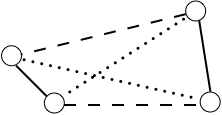
\includegraphics[scale=0.55]{FiguresGraph/perfectmatchingAll}
       \caption{The three different perfect matchings in the $4$-node
         clique $\k_4$: the matchings' edges are drawn, respectively,
         with bold lines, dashed lines, and dotted lines.}
%of one matching are drawn in bold;
% The optimal one is represented in bold (the two others are in dashed and dot lines).}
  \label{fig:AllPerfectMatchings}
\end{center}
\end{figure}
As the figure illustrates, $\k_4 = \k_{2 \cdot 2}$ can be viewed as a
$4$-cycle (drawn with bold and dashed lines), augmented by two
``cross-edges'' (drawn with dotted lines).  Easily, then, $\k_4$
admits $3$ different perfect matchings, which can be identified (and
specified) by the edge that contains the northwesterly node---call it
$v$---in the figure.  Node $v$ has the choice of three nodes to
``boldly'' match with. (In the figure, $v$ has chosen the
southwesterly node as its ``bold'' match.)  Once $v$ has chosen its
match, there is only one viable choice for the second edge in the
matching.  Thus, $M_2=3$.

We jump now to the case of any arbitrary $k > 2$.  We remark that
there are precisely $2k-1$ nodes of $\k_{2k}$ that node $1$ can
``choose'' as its mate in a perfect matching.  Once we set node $1$
and its chosen mate aside, we confront an independent instance of the
problem with parameter $k-1$, i.e., the problem of counting the number
of perfect matchings in $\k_{n-2} = \k_{2k-2}$.  We thereby note that
as $k$ grows, the quantity $M_k$ obeys the following recurrence:
\[ M_k \ = \ (2k-1) \cdot M_{k-1} \]
In other words:

\hspace*{.25in}{\em $M_k$ is the product of the first $k$ odd numbers.}
%$N_1=1$, $N_2=3$, $N_3=3 \times 5=15$, $N_4=3 \times 5 \times 7=115$, etc..

\noindent
To gauge the growth rate of $M_k$, we concentrate on cases $k > 2$ and
ignore the $\lfloor k/2 \rfloor$ smallest odd numbers.  We then
replace each of the remaining odd numbers by its smallest possible
value.  We thereby find that
\[
M_k \ \ =    \ \ \prod_{i=1}^k \ (2i-1)
    \ \ \geq \ \ \prod_{\lceil k/2 \rceil}^k \ (2i-1)
    \ \ \geq \ \ \left( 2 \lceil k/2 \rceil -1 \right)^{k/2}
    \ \ >    \ \ k^{k/2}
\]
In summary, $M_k$ grows exponentially with the parameter $k$, as claimed.
\qed
\end{proof}


\bigskip

The two families of graphs we have just discussed, cycles and cliques,
are recommended to our attention by their structural simplicity---they
epitomize, respectively, the most sparse way (the cycle) and the most
dense way (the clique) to completely interconnect $n$ nodes.  The
remainder of this section is devoted to three graph-structures that
are structurally more complex than cycles and cliques, which have been
designed to meet specific needs within the real technological world of
computing and communicating.  Indeed, the three upcoming graph
families are among the most important ones when discussing parallel
and distributed computing (PDC, for short).  All three families have
been used both to design computer architectures that support PDC and
to craft algorithms that exploit the potential efficiencies---in
computation and communication---that one can achieve using PDC.

\subsubsection{The mesh ($\m_{m,n}$) and torus ($\widetilde{\m}_{m,n}$) networks}
\label{sec:mesh-torus}
\index{mesh and torus networks}

For positive integers $m, n \in \N^+$, both the $m \times n$ {\it mesh
  (network)} $\m_{m,n}$ and the $m \times n$ {\it toroidal network}
(or, {\it torus}) $\widetilde{\m}_{m,n}$ have {\it node-set}
\begin{eqnarray*}
\n_{\fm_{m,n}} \ = \ \n_{\widetilde{\fm}_{m,n}}
  & = & 
\{1, \ 2, \ldots, \ m\} \ \times \ \{1, \ 2, \ldots, \ n\} \\
  & = & 
\big\{ \langle i, \ j \rangle \ \ | \ \ 
\big[ i \in \{1, \ 2, \ldots, \ m\} \big], \ \
\big[ j \in \{1, \ 2, \ldots, \ n\} \big]
\big\}
\end{eqnarray*}

\begin{itemize}
\item
$\m_{m,n}$ has $(m-1)n \ + \ (n-1)m$ edges; its {\it edge-set} is
\begin{eqnarray*}
\e_{\fm_{m,n}} & = & 
\big\{
\{ \{ i, j \}, \ \{ i+1, j \} \ \ | \ \
1 \leq i < m, \ \ 1 \leq j \leq n \} \\
  &  & \hspace*{.1in} \cup
\{ \{ i, j \}, \ \{ i, j+1 \} \ \ | \ \
1 \leq i \leq m, \ \ 1 \leq j < n \}
\big\}
\end{eqnarray*}

  \begin{itemize}
  \item
    \begin{itemize}
    \item
The subgraph of $\m_{m,n}$ defined by the node-set
\[ \{ \langle i, \ j \rangle  \ \ | \ \ \left[i \in \{1, 2, \ldots,
  m\}\right], \ \ \left[1 \leq j < n\right]\}
\]
and all edges both of whose endpoints belong to that set is called the
$i$th {\it row} of $\m_{m,n}$
\index{row of a mesh graph}
\index{mesh graph!row}
Dually, the subgraph of $\m_{m,n}$ defined by the node-set
\[ \{ \langle i, \ j \rangle  \ \ | \ \ \left[j \in \{1, 2, \ldots,
  n\}\right], \ \ \left[1 \leq i < m\right] \}
\]
and all edges both of whose endpoints belong to that set is called the
$j$th {\it column} of $\m_{m,n}$.
\index{column of a mesh graph}
\index{mesh graph!column}
     \item
Nodes $\langle 1, \ 1 \rangle$, $\langle 1, \ n \rangle$, $\langle m,
\ 1 \rangle$, and $\langle m, \ n \rangle$ are the {\it corner nodes}
(or, just {\it corners}) of $\m_{m,n}$.
\index{corner (node) of a mesh graph}
\index{mesh graph!corner (node)}
     \item
The path-graph consisting of the node-set
\[ \{ \langle 1, \ 1 \rangle, \ \langle 1, \ 2 \rangle, \ldots, \
\langle 1, \ n \rangle \}
\]
together with all edges of $\m_{m,n}$ both of whose endpoints belong
to this set, is the {\it top edge} of $\m_{m,n}$.
\index{top edge of a mesh graph}
\index{mesh graph!top edge}

The other edges of $\m_n$ are defined analogously:

\smallskip

The {\it bottom edge} of $\m_{m,n}$ is the path-graph built upon the
node-set
\[ \{ \langle m, \ 1 \rangle, \ \langle m, \ 2 \rangle, \ldots, \
\langle m, \ n \rangle \}
\]
\index{bottom edge of a mesh graph}
\index{mesh graph!bottom edge}

The {\it left edge} of $\m_{m,n}$ is the path-graph built upon the
node-set
\[ \{ \langle 1, \ 1 \rangle, \ \langle 2, \ 1 \rangle, \ldots, \
\langle m, \ 1 \rangle \}
\]
\index{left edge of a mesh graph}
\index{mesh graph!left edge}

The {\it right edge} of $\m_{m,n}$ is the path-graph built upon the
node-set
\[ \{ \langle 1, \ n \rangle, \ \langle 2, \ n \rangle, \ldots, \
\langle m, \ n \rangle \}
\]
\index{left edge of a mesh graph}
\index{mesh graph!right edge}
     \end{itemize}

  \item \index{mesh graph!node-degree}
$\m_{m,n}$ is {\em not} a regular graph.  Its corner nodes each has
    degree $2$; its non-corner edge nodes each has degree $3$; its
\index{internal node of a mesh graph}
\index{mesh graph!internal node}
{\em internal nodes}---which are all non-edge nodes---each has degree
$4$

  \item \index{mesh graph!undirected diameter}
The diameter of $\m_{m,n}$ is $m+n-2$, as witnessed by the distance
between nodes $\langle 1, \ 1 \rangle$ and $\langle 2, \ n \rangle$.
  \end{itemize}

\item
$\widetilde{\m}_{m,n}$ has $2mn$ arcs; its {\it arc-set} is
\begin{eqnarray*}
\a_{\widetilde{\m}_{m,n}} & = &
\big\{
\{ (\langle i, \ j \rangle \rightarrow \langle i+1 \bmod m, \ j
\rangle) \ \ | \ \ 1 \leq i \leq m, \ \ 1 \leq j \leq n \} \\
  &  & \hspace*{.1in} \cup
\{ (\langle i, \ j \rangle \rightarrow \langle i, \ j+1 \bmod n
\rangle) \ \ | \ \ 1 \leq i \leq m, \ \ 1 \leq j \leq n \}
\big \}
\end{eqnarray*}

  \begin{itemize}
  \item
The subgraph of $\widetilde{\m}_{m,n}$ defined by the node-set
\[ \{ \langle i, \ j \rangle  \ \ | \ \ \left[i \in \{1, 2, \ldots,
  m\}\right], \ \ \left[1 \leq j \leq n\right]\}
\]
and all edges both of whose endpoints belong to that set is called the
$i$th {\it row} of $\widetilde{\m}_{m,n}$
\index{torus graph!row}
Dually, the subgraph of$\widetilde{\m}_{m,n}$ defined by the node-set
\[ \{ \langle i, \ j \rangle  \ \ | \ \ \left[j \in \{1, 2, \ldots,
  n\}\right], \ \ \left[1 \leq i \leq m\right] \}
\]
and all edges both of whose endpoints belong to that set is called the
$j$th {\it column} of $\widetilde{\m}_{m,n}$.
\index{torus graph!column}
  \item
$\widetilde{\m}_{m,n}$ is a regular network; each node has degree $4$.
    Despite the fact that $\widetilde{\m}_{m,n}$ is an {\em
      undirected} graph, its arcs are commonly referred to via an
    anthropomorphic labeling, either as ``up, down, left, and right''
    or as ``north, south, west, and east''.
  \item \index{mesh graph!directed diameter}
$\widetilde{\m}_{m,n}$'s diameter is $\lfloor m/2 \rfloor \ + \
\lfloor n/2 \rfloor$.  This can be verified in analogy to the diameter
of the cycle-graph $\cc_n$.
  \end{itemize}
\end{itemize}

\begin{figure}[hbt]
\begin{center}
       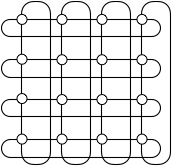
\includegraphics[scale=0.6]{FiguresGraph/torus}
       \caption{The $4 \times 4$ torus.}
  \label{fig:torus}
\end{center}
\end{figure}

\subsubsection{The (boolean) hypercube network $\q_n$}
\index{boolean hypercube}
\index{hypercube}

The graphs we focus on in this section have had a major impact on the
world of coding, especially in regard to codes that are {\em error
  correcting} \cite{PetersonW81}, and the world of computing,
especially in regard to parallel and distributed computing
\cite{JohnssonH1989, SaadS89, Schwartz80}.  The cited sources give a
range of perspectives on the importance of {\it hypercube networks.}

\index{order-$n$ boolean hypercube}
The {\it order-$n$ boolean hypercube}, traditionally denoted $\q_n$,
is the $2^n$-node graph defined as follows.
\begin{itemize}
\item
{\it The recursive definition}. 
\index{order-$n$ boolean hypercube!recursive definition}
  \begin{itemize}
  \item
The order-$0$ boolean hypercube, $\q_0$, has a single node, and no
edges.
  \item
The order-$(k+1)$ boolean hypercube, $\q_{k+1}$, is obtained by taking
two copies of $\q_k$, call them $\q_k^{(1)}$ and $\q_k^{(2)}$, and
creating an edge that connects each node of $\q_k^{(1)}$ with the
corresponding node of $\q_k^{(2)}$.
  \end{itemize}
For illustration:
  \begin{itemize}
  \item
$\q_1$ consists of two nodes connected by a single edge.
  \item
$\q_2$ can be viewed as a ``square'', or equivalently, a copy of $\cc_4$.
  \item
$\q_3$ can be viewed as a ``cube'', i.e., as two copies of $\cc_4$
    with edges connecting corresponding nodes: Each of the following
    pairs of nodes are connected by an edge: the upper right
    corner-nodes, the upper left corner-nodes, the lower right
    corner-nodes, and the lower left corner-nodes.
  \end{itemize}

\item
{\it The direct definition}.
For each $n \in \N$, the nodes of the order-$n$ boolean hypercube,
$\q_n$, are all length-$n$ binary strings.  For illustration:
\index{order-$n$ boolean hypercube!direct definition}
\begin{eqnarray*}
\n_{{\fq}_0}
  & = & 
\{ \varepsilon \}, \ \ \mbox{ the length-$0$ {\em null string}} \\ 
\n_{{\fq}_1}
  & = &
\{ 0, \ 1 \} \\
\n_{{\fq}_2}
  & = & \{ 00, \ 01, \ 10, \ 11 \} \\
\n_{{\fq}_3}
  & = & \{ 000, \ 001, \ 010, \ 011, \ 100, \ 101, \ 110, \ 111 \} 
\end{eqnarray*}
The iteration-based construction of big hypercubes from the next
smaller ones is illusrated in Fig.~\ref{fig:hypercube}.
\begin{figure}[hbt]
\begin{center}
       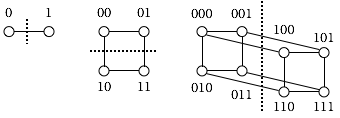
\includegraphics[scale=0.6]{FiguresGraph/hypercube}
\caption{The iteration-based construction of order-$n$ hypercubes:
  Take two copies of the order-$(n-1)$ hypercube.  Prepend a $0$ to
  the node-labels of the first copy and a $1$ to the node-labels of
  the second copy.}
  \label{fig:hypercube}
\end{center}
\end{figure}

Easily, for each value of $n$, $\q_n$ has $2^n$ nodes, for this is the
number of length-$n$ binary strings.

\medskip

For each value of $n$, each edge of $\q_n$ connects two node-strings
that differ in precisely one position.  This means that $\q_n$ has $n
2^{n-1}$ edges: To wit, each of its $2^n$ nodes has $n$ neighbors, so
the quantity $n 2^n$ counts each of $\q_n$'s edges twice---one for
each endpoint.  For illustration:
\begin{eqnarray*}
\a_{{\fq}_1}
  & = &
\big\{ \{ 0, \ 1 \} \big\} \\
\a_{{\fq}_2}
  & = & \big\{
\{ 00, \ 01 \}, \ \{ 00, \ 10\}, \
\{ 01, \ 11 \}, \ \{ 10, \ 11\} 
\big\} \\
\a_{{\fq}_3}
  & = & \big\{ 
\{000, \ 001\}, \
\{000, \ 010\}, \
\{000, \ 100\}, \
\{001, \ 011\}, \\
  &  & \hspace*{.2in}
\{001, \ 101\}, \
\{010, \ 011\}, \
\{010, \ 110\}, \
\{100, \ 101\}, \\
  &  & \hspace*{.2in}
\{100, \ 110\}, \
\{101, \ 111\}, \
\{011, \ 111\}, \
\{110, \ 111\}
\big\}
\end{eqnarray*}
\end{itemize}

\medskip

\noindent
It is easy to observe $\q_n$'s basic structural properties.
\begin{itemize}
\item \index{hypercube!node-degree}
$\q_n$ is a regular network: each of its $2^n$ nodes has degree $n$.

This follows from the fact that each arc of $\q_n$ rewrites a single
bit-position in the length-$n$ binary string that is the arc's source
node.

\item \index{hypercube!diameter}
$\q_n$ has diameter $n \ = \ \ln(|\n_{\fq_n}|)$.\footnote{Recall that
  $\ln n = \log_2 n$; see Section~\ref{sec:logarithmic-fns}.}

We address this issue formally.
\end{itemize}

\begin{prop}
\label{thm:hypercube-diameter}
For all $n \in \N^+$, $\q_n$ has diameter $n \ = \ \ln(|\n_{\fq_n}|)$.
\end{prop}

\begin{proof}
We prove this diameter bound by construction.  Focus on two arbitrary
nodes of $\q_n$:
\[ x \ = \ \alpha_1 \alpha_2 \cdots \alpha_n \ \ \ \mbox{ and } \ \ \
y \ = \ \beta_1 \beta_2 \cdots \beta_n
\]
One of the several paths in $\q_n$ from $x$ to $y$ is described
schematically as the following left-to-right, bit-by-bit rewriting of
$x$ as $y$ using arcs of $\q_n$
\[
x \ = \ \alpha_1 \alpha_2 \cdots \alpha_n \ \rightarrow \
\beta_1 \alpha_2 \cdots \alpha_n \ \rightarrow \
\beta_1 \beta_2\cdots \alpha_n \ \rightarrow \cdots \rightarrow\ 
\beta_1 \beta_2 \cdots \beta_n \ = \ y
\]
Since each bit of each string is rewritten once, the bound follows.
\qed
\end{proof}

\medskip

The fact that $\q_n$'s diameter is {\em logarithmic} in its size makes
$\q_n$ an efficient network for many tasks related to parallel
computing and communication.

\bigskip

A powerful avenue for understanding the structure of a given family of
networks is to understand how the perceived ``shape'' of graphs in the
family can apparently change just by relabeling/renaming the nodes, or
the edges/arcs, of the graphs.  The formal mechanism for studying such
relabelings/renamings is the concept of {\it graph isomorphism}.
\index{graph isomorphism} Let $\g$ and $\h$ be undirected graphs that
have the same numbers of nodes and edges.  (The following definition
can easily be adapted to deal with {\em directed} graphs.)  An {\it
  isomorphism} between $\g$ and $\h$ is a {\em
  bijection}\footnote{Recall, from Chapter~\ref{ch:sets-BA-logic} that
  a bijection is a function that is one-to-one (i.e., injective) and
  onto (i.e., surjective).}
\[ \beta: \n_{\fg} \ \leftrightarrow \ \n_{\fh} \]
such that
\begin{itemize}
\item
For each edge $\{ u,v \}$ of $\g$ (i.e., $\{ u,v \} \in \e_{\fg}$),
the doubleton set $\{ \beta(u), \beta(v) \}$ is an edge of $\h$ (i.e.,
$\{ \beta(u), \beta(v) \} \in \e_{\fh}$).
\item
For each edge $\{ x,y \}$ of $\h$ (i.e., $\{ x,y \} \in \e_{\fh}$),
the doubleton set $\{ \beta^{-1}(x), \beta^{-1}(y) \}$ is an edge of $\g$ (i.e.,
$\{ \beta^{-1}(x), \beta^{-1}(y) \} \in \e_{\fg}$).
\end{itemize}
We can immediately exemplify this notion via the following example.

\begin{prop}
The order-$4$ hypercube $\q_4$ is \textit{isomorphic} to the $4 \times
4$ torus $\widetilde{\m}_{4,4}$.
\end{prop}

\begin{figure}[hbt]
\begin{center}
       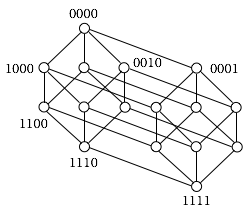
\includegraphics[scale=0.6]{FiguresGraph/Isomorphism1}
       \caption{A representation of $\q_4$.}
  \label{fig:isomorphism1}
\end{center}
\end{figure}

\begin{figure}[hbt]
\begin{center}
       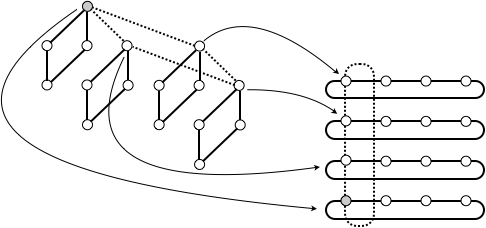
\includegraphics[scale=0.5]{FiguresGraph/Isomorphism2}
       \caption{Transformation of $\q_4$ to a $4 \times 4$ torus.}
  \label{fig:isomorphism2}
\end{center}
\end{figure}

A graphical proof is depicted in Fig.~\ref{fig:isomorphism1}  and ~\ref{fig:isomorphism2} and 
We relegate the formal proof of this result to a Exercise, supplying as a
hint the coding scheme (or, bijection) depicted in
Fig.~\ref{fig:toruslabel}.
\begin{figure}[hbt]
\begin{center}
       \includegraphics[scale=0.6]{FiguresGraph/toruslabel}
\caption{Sketching the coding scheme that yields an isomorphism
  between the order-$4$ hypercube $\q_4$ and the $4 \times                          
4$ torus $\widetilde{\m}_{4,4}$.}
  \label{fig:toruslabel}
\end{center}
\end{figure}


\subsubsection{The de Bruijn network $\d_n$}
\label{sec:deBruijn-network}
\index{de Bruijn network}
\index{de Bruijn graph}

While the family of hypercube networks has few competitors in the
world of parallel and distributed computing, in terms of performance
and ease of designing algorithms, it does have one major shortcoming
regarding its realization in hardware.  The basic problem is that the
order-$n$ hypercube has large node-degrees, specifically logarithmic
in the size of the network.  This feature makes the hypercubes actual
performance much lower than its theoretical performance.
Specifically, the size of the hypercube grows exponentially with the
common degrees of the network's nodes---this is the ``inverse'' way
of talking about logarithmic node-degrees---while the space in which
we (and our computers) live grows only cubically with linear
distance.  The resulting disparity means that the wires in a large
hypercube must inevitably be very long---in contrast to the unit-size
of idealized network-edges.  Consequently, electrical signals within a
large hyeprcube must travel long distances, which means that the
physical computer is much slower than its idealized version.  (One
finds a more technical discussion of this phenomenon in
\cite{Ullman84}.)

The preceding shortcoming of hypercubes led researchers to seek a
family of networks whose node-degrees stay constant even as one
deploys successively larger instances of the network.  A candidate
such network was discovered within the domain of coding theorists (as,
coincidentally, was the hypercube).  

In the mid-20-century, Dutch mathematican Nicolaas Govert de Bruijn
\index{de Bruijn, Nicolaas Govert} discovered a way to generate
compact sequences that contain all possible strings of a prespecified
length.  Focussing on {\em binary} strings---although de Bruijn's
strategy works for any finite alphabet---de Bruijn could generate a
string of length $2^n +n-1$ that contains every length-$n$ binary
string as a substring.  Quite appropriately, such a string is called a
{\it de Bruijn sequence}. \index{de Bruijn sequence} It is not obvious
that de Bruijn sequences exist for every $n$, but we now plant the
seeds of a proof that they do.  We begin by illustrating two sample
sequences in (\ref{eqn:deBruijn-seq}).
\begin{equation}
\label{eqn:deBruijn-seq}
\begin{array}{|l||c|c|}
\hline
n & \mbox{\sc Length-$n$ binary strings}
    & \mbox{\sc Order-$n$ de Bruijn sequence} \\
\hline
\hline
1 &
00, \ 01, \ 10, \ 11  & 00110 \\
\hline
2 &
\begin{array}{l}
000, \ 001, \ 010, \ 011, \\
100, \ 101, \ 110, \ 111 
\end{array}
  & 0001110100 \\
\hline
\end{array}
\end{equation}
The table in (\ref{eqn:deBruijn-seq}) spawns many interesting
questions:
\begin{itemize}
\item
Do de Bruijn sequences exist for every $n$?
\item
If so, 
  \begin{itemize}
  \item
How does one compute them?
  \item
Can one always find a de Bruijn sequence of length $2^n +n-1$?
  \item
Can one find de Bruijn sequences of length $< 2^n +n-1$?
  \end{itemize}
 {\Arny (SOME GOOD EXERCISES HERE)}  
\end{itemize}
The answers to all of these questions---and the connection of de
Bruijn sequences to the current chapter---reside in the family of
directed graphs called {\it de Bruijn graphs} (or, {\it networks}).
\index{de Bruijn graph} \index{de Bruijn network} (The term used
varies by intended application---mainly, coding theory and [the
  interconnection networks of] parallel computer architectures.  We
use the names interchangeably.)

\begin{figure}[hbt]
\begin{center}
       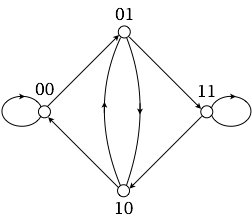
\includegraphics[scale=0.6]{FiguresGraph/dB2by2}
       \caption{The $4$-node, order-$2$ de Bruijn network.}
  \label{fig:dB2by2}
\end{center}
\end{figure}

\begin{figure}[hbt]
\begin{center}
       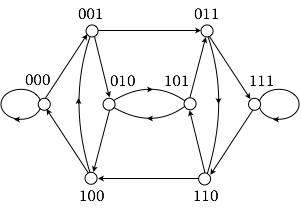
\includegraphics[scale=0.6]{FiguresGraph/dB2by3}
       \caption{The $8$-node, order-$3$ de Bruijn network.}
  \label{fig:dB2by3}
\end{center}
\end{figure}

For every integer $n \in \N^+$, the {\it order-$n$ de Bruijn network}
is the {\em directed} graph $\d_n$ whose nodes comprise the set of
length-$n$ binary strings\footnote{While {\em binary} de Bruijn
  networks are the most frequently encountered ones, one can also find
  de Bruijn networks whose nodes comprise all length-$n$ strings over
  larger finite alphabets.  Such extended families also find
  applications in coding theory.}  The sets $\n_{\fd_2}$ and
$\n_{\fd_3}$ appear in (\ref{eqn:deBruijn-seq}).


$\d_n$ is a regular directed graph; its nodes all have in-degree $2$
and outdegree-$2$.  Each node of $\d_n$ is a binary string of
length $n \geq 1$; hence it can be written in the form $\beta x$,
where $\beta \in \{0, \ 1\}$ is a {\it bit} (short for {\it binary
  digit}) and $x$ is a length-$(n-1)$ binary string.

The $2^{n+1}$ arcs of $\d_n$ come in pairs specified as follows.  For
each $\beta \in \{0,1\}$ and for each length-$(n-1)$ binary string
$x$, $\d_n$ has the two arcs
\[ (\beta x \rightarrow x0) \ \ \ \mbox{ and } \ \ \ 
(\beta x \rightarrow x1)
\]
We enumerate $\a_{\fd_3}$ in (\ref{eqn:deBruijn-arcs}).
\begin{equation}
\label{eqn:deBruijn-arcs}
{\small
\begin{array}{|ccccc|}
\hline
\mbox{\sc Source node} & & \mbox{\sc Target node} & & \mbox{\sc Target node} \\
\hline \hline
{\displaystyle
\left.
\begin{array}{c}
000 \\
001 \\
010 \\
011 \\
100 \\
101 \\
110 \\
111
\end{array}
\right\}
} &
\mbox{\sc goes to} 
  &
{\displaystyle
\left\{
\begin{array}{c}
000 \\
010 \\
100 \\
110 \\
001 \\
011 \\
101 \\
111
\end{array}
\right.
}
  &
\mbox{\sc and to}
  &
{\displaystyle
\left\{
\begin{array}{c}
001 \\
011 \\
101 \\
111 \\
000 \\
010 \\
100 \\
110
\end{array} 
\right.
}
 \\
\hline
\end{array}
}
\end{equation}

For each $n \in \N^+$, $\d_n$ has diameter $n$.  To see why this is
true, note that following any one of $\d_n$'s arcs, say from node $x$
to node $y$, consists of ``rewriting'' the length-$n$ string $x$ as
the length-$n$ string $y$.  The diameter bound therefore follows by
showing that, for any two string-nodes of $\d_n$, say node $u$ and
node $v$, one can rewrite string $u$ as string $v$ by traversing a
sequence of arcs---i.e., a directed path---of length at most $n$.
Observe, for instance, that the path in $\d_3$ described schematically
as follows
\[ 000 \ \rightarrow \ 001 \ \rightarrow \ 011 \ \rightarrow \ 111 \]
leads node $000$ to node $111$, by rewriting string $000$ as string
$111$.  The diameter bound is now an immediate consequence of the
following result.  The result builds upon a notion that we have not
yet encountered but will study in some detail in
Section~\ref{sec:Hamiltonian-cycle}.
\index{graphs!Hamiltonian cycle} \index{Hamiltonian cycle}.

A {\it Hamiltonian cycle} in an $n$-node graph $\g$ is a length-$n$
cycle that contains every node of $\g$ precisely once.  A {\it
  directed Hamiltonian cycle} in an $n$-node digraph $\h$ is a
length-$n$ directed cycle that contains every node of $\h$ precisely
once.

\begin{prop}
\label{thm:deBruijn-Hamiltonian}
For all $n \in \N^+$, $\d_n$ contains a {\em directed Hamiltonian
  cycle}, 
\index{directed Hamiltonian cycle in a digraph}
i.e., a length-$2^n$ directed cycle of the form
\begin{equation}
\label{eq:deBruijn-cycle}
 x \ \rightarrow \ y_1 \ \rightarrow \ y_2 \ \rightarrow \cdots
\ \rightarrow \ y_{2^n-1} \ \rightarrow \ x
\end{equation}
that contains every node of $\d_n$ precisely once; i.e.:
\begin{itemize}
\item
$\{x, \ y_1, \ y_2, \ldots, \ y_{2^n-1}\} \ = \ \n_{\fd_n}$.
\item
All of the ``$y$-nodes'' that appear in cycle
(\ref{eq:deBruijn-cycle}) differ from $x$ and from each other.
\end{itemize}
\end{prop}

The simplest proof of this result has two steps, each of which
introduces a topic we have not yet developed.

\medskip

\noindent {\bf (1)}
%
For any directed graph $\g$, the {\it line digraph} \index{line graph}
\index{line digraph} of $\g$, denoted $\Lambda(\g)$, is the following
directed graph.
\begin{itemize}
\item
The nodes of $\Lambda(\g)$ are the arcs of $\g$:
\[ \n_{{\cal L}({\cal G})} \ = \ \a_{\fg} \]
\item
For each pair of arcs of $\g$ of the form
\[ \big[a_{x,y} = (x \ \rightarrow \ y) \big] \ \ \ \mbox{ and } \ \ \ 
\big[a_{y,z} = (y \ \rightarrow \ z) \big]
\]
i.e, arcs such that the endpoint of the first arc is the source of the
second arc, $\Lambda(\g)$ contains an arc $(a_{x,y} \ \rightarrow
\ a_{y,z})$.
\end{itemize}
The relevance of this topic to this section is that the line graph of
every de Bruijn network $\d_n$ is the ``next bigger'' de Bruijn
network, $\d_{n+1}$.  Let us verify this claim.

\begin{prop}
\label{thm:deBruin-linegraph}
For all $n \in \N^+$,
$\d_{n+1}$ is the line digraph of $\d_n$: $\d_{n+1} \ = \ \Lambda(\d_n)$.
\end{prop}

\begin{proof}
Each node of $\Lambda(\d_n)$ is an arc of $\d_n$, hence has the form
\[ (\beta x \ \rightarrow \ x \gamma) \]
for $x$ a length-$(n-1)$ binary string and $\beta, \gamma \in
\{0,1\}$.  Let us associate node $\beta x \gamma$ of $\d_{n+1}$ with
this node of $\Lambda(\d_n)$.

\smallskip

Note first that each arc of $\d_{n+1}$ has the form
\[ (\delta y \varepsilon \ \rightarrow \ y \varepsilon \varphi), \]
where $y$ is a length-$(n-2)$ binary string and $\delta, \varepsilon,
\varphi \in \{0,1\}$.  By our association of nodes of $\d_{n+1}$ with
arcs of $\d_n$, this arc of $\d_{n+1}$ does, indeed, correspond to two
successive arcs of $\d_n$.   The first of these successive arcs
{\em enters} node $y \varepsilon$ of $\d_n$; the second {\em leaves}
that node.

Note next that, given any two successive arcs of $\d_n$, say
\[
(\rho \sigma z \ \rightarrow \ \sigma z \tau) \ \ \ \mbox { and } \ \ \
(\sigma z \tau \ \rightarrow \  z \tau \xi)
\]
where $z$ is a length-$(n-2)$ binary string and $\rho, \sigma, \tau,
\xi \in \{0,1\}$, there is, indeed, an arc of $\d_{n+1}$ of the form
\[ (\rho \sigma z \tau \ \rightarrow \ \sigma z \tau \xi) \]
This means that the digraph $\d_{n+1}$ is identical to the digraph
$\Lambda(\d_n)$, modulo a renaming of nodes and arcs.\footnote{Technically,
  we are asserting that the digraphs ${\cal D}_{n+1}$ and ${\cal
    L}({\cal D}_n)$ are {\it isomorphic} to one another.  The topic of
  graph isomorphism is beyond the scope of this text, but our informal
  description provides all the details one would need to formalize the
  described isomorphism.}

The described correspondence between the nodes and arcs of $\d_{n+1}$
and $\Lambda(\d_n)$ completes the proof.  \qed
\end{proof}

\begin{figure}[hbt]
\begin{center}
       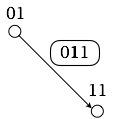
\includegraphics[scale=0.6]{FiguresGraph/dBlabelEdge}
\caption{Illustrating how to label each arc of a de Bruijn network by
  concatenating the labels of the nodes incident to the arc and
  compacting the common intermediate bits.  In the depicted example,
  the node-labels $01$ and $11$ combine to yield the arc-label $011$.}
  \label{fig:dBlabelEdge}
\end{center}
\end{figure}

\medskip

\noindent {\bf (2)}
{\it Eulerian cycles (or tours)}. \index{Eulerian cycle}
\index{Eulerian tour} A {\it directed Eulerian cycle} in a digraph
$\g$ is a directed cycle that contains each arc of $\g$ precisely
once.  We will see, later in this chapter, a truly elementary
argument, based on node-degrees, which proves that every de Bruijn
digraph has a directed Eulerian cycle.  This demonstration will
combine with Proposition~\ref{thm:deBruin-linegraph} to complete the
proof of Proposition~\ref{thm:deBruijn-Hamiltonian}.  \qed
%\end{proof}

\bigskip

Stepping back from the structural specifics of $\d_n$, we now see that
de Bruijn networks provide us with a {\em
  bounded-degree---specifically, a degree-$2$} family of networks each
of whose constituent graphs has {\em logarithmic diameter}!  In this
regard, at least, de Bruijn networks have exactly the same
cost-performance as hypercubes---i.e., $2^n$-node graphs with diameter
$n$---with bounded degrees.  Even more dramatic, it has been shown
that sophisticated algorithmic techniques can achieve roughly
equivalent computational efficiency, on a broad range of significant
computational problems, using de Bruijn networks as using like-sized
hypercubes \cite{AnnexsteinBR90, BermondP89, Ullman84}.


\section{Path and Cycle Discovery Problems in Graphs}
\label{sec:path-cycle-problems}

Just as various genres of {\it spanning trees} are used to
``summarize'' aspects of the connectivity structure of a connected
graph $\g$, various genres of {\it paths} and {\it cycles} in $\g$ are
often useful to ``summarize'' aspects of $\g$'s traversal structure.
This section is devoted to a range of problems related to determining
the existence in a graph $\g$ of a path or a cycle that {\em
  completely} ``summarizes'' $\g$'s traversal structure, either by
containing each node of $\g$ precisely once or by containing each edge
of $\g$ precisely once.  We shall generally focus in this section only
on {\em undirected} paths and cycles in {\em undirected}, {\em
  unweighted} graphs.  Extrapolating the notions we discuss to their
directed analogues in directed and/or weighted graphs, will be
accomplished via carefully crafted exercises.  In a similarly, but
simpler, vein, we shall generally discuss only prolems concerning {\em
  cycles}, leaving to the reader the analogous notions that concern
paths.  We begin by delimiting the two main classes of cycle-discovery
problems that we study in this section.

\smallskip

{\it Eulerian cycles (or, tours)}.  A cycle in a graph $\g$ that
traverses each of $\g$'s edges precisely once is called an {\it
  Eulerian cycle},\index{graphs!Eulerian cycle} \index{Eulerian cycle}
(or, often, an {\it Eulerian circuit}).  \index{graphs!Eulerian
  circuit} \index{Eulerian circuit} The edge-exhausting
cycles/circiuts/tours referred to by these several names were
introduced as a topic of study in 1736 by the Swiss mathematician
\index{Euler, Leonhard} Leonhard Euler, whose name we have already
encountered multiple times.  Euler allegedly discovered the topic
while contemplating how to design a tour of the town of K\"{o}nigsberg
that would cross each of the town's bridges precisely once.  The quest
for Eulerian cycles in graphs is, thus, one of the oldest problems in
the fields now called {\it Operations Research} and {\it graph
  theory}.  (An edge-exhausting {\em path} in $\g$ is referred to in
the obvious analogous way.)  When one views an Eulerian cycle as a
``map'' for traversing a graph---as did Euler when contemplating this
problem---one often calls the cycle an {\it Eulerian tour}.
\index{graphs!Eulerian tour} \index{Eulerian tour} Traditionally, a
graph that admits an Eulerian cycle is said to be {\it
  Eulerian}. \index{graphs!Eulerian} \index{Eulerian graph}

\medskip

Dually: A cycle in a graph $\g$ that encounters each of $\g$'s nodes
precisely once is called a {\it Hamiltonian cycle},
\index{graphs!Hamiltonian cycle} \index{Hamiltonian cycle} (or, often,
a {\it Hamiltonian circuit}). \index{graphs!Hamiltonian circuit}
\index{Hamiltonian circuit} This cycle-discovery problem is named in
honor of the British mathematician William Rowan Hamilton,
\index{Hamilton, William Rowan} who is credited with inventing the
concept in the mid-19th century.  (A node-exhausting {\em path} in
$\g$ is referred to in the obvious analogous way.)  When one views a
Hamiltonian cycle as a ``map'' for traversing a graph, one often calls
the cycle a {\it Hamiltonian tour}.  \index{graphs!Hamiltonian tour}
\index{Hamiltonian tour} Traditionally, a graph that admits a
Hamiltonian cycle is said to be {\it
  Hamiltonian}. \index{graphs!Hamiltonian} \index{Hamiltonian graph}

\medskip

Despite the conceptual duality between the edge-encountering goal that
underlies Eulerian paths and cycles, on the one hand, and the
node-encountering goal that underlies Hamiltonian paths and cycles,
these two graph-traversing goals differ in virtually every significant
respect.  It is rather easy to characterize the family of graphs that
admit Eulerian tours and to find such a tour if it exists
(Section~\ref{sec:EulerianCycle}); in contrast, there is no known
characterization of the family of graphs that admit Hamiltonian tours,
and the computational problem of efficiently determining whether a
graph admits such a tour is one of the major classical problems in the
field of computational complexity  (Section~\ref{sec:Hamiltonian-cycle}).

%%%%%%%%%%%%%%%%%%%%%%%%%%%%%%%%%%%%%%%%%%%%%%%%%%%%

\subsection{Eulerian Cycles and Paths}
\label{sec:EulerianCycle}

The main results in this section characterize the families of directed
and undirected graphs that admit an {\it Eulerian cycle} or an {\it
  Eulerian path}.  The proofs of these characterizations are
constructive: they consist of algorithms that efficiently find such a
cycle or such a path when one exists.  We focus on graphs that are
connected: the algorithms we present can actually be adapted to find
an {\it Eulerian cycle} or an {\it Eulerian path} in each connected
component of a general graph.  As we embark on our adventure, we note
that the problem of finding an Eulerian cycle in a graph $\g$ is
equivalent to the problem of drawing $\g$ without ever lifting one's
pencil. \index{graphs!drawing without lifting pencil}

%\subsubsection{Characterizing Eulerian graphs, and finding Eulerian tours}
%\label{sec:eulerian-cycle-path}

There is a simple and elegant characterization of graphs that admit
Eulerian cycles and paths, which is accompanied by a simple and
efficent algorithm for testing a given graph for finding such a tour
in a graph that admits one.  We encapsulate four versions of the
desired result in the following statement.

\begin{prop}[Eulerian Cycles]
\label{thm:eulerian-cycle}
{\bf (a)}
An undirected graph $\g$ admits an Eulerian cycle if, and only if,
$\g$ is connected and every node of $\g$ has even degree.

{\bf (b)}
A directed graph $\h$ admits a directed Eulerian cycle if, and only if,
$\h$ is connected and, for every node $v$ of $\g$,
$\mbox{\sc indegree}(v) \ = \ \mbox{\sc outdegree}(v)$.
\end{prop}

\begin{proof}
The {\em necessity} of the conditions in both parts {\bf (a)} and {\bf
  (b)} is established thus.
\begin{itemize}
\item
By definition, a graph that is not connected does not admit any cycle.
\item
Each cycle that a graph admits accounts for two edges per node,
because the cycle must ``enter'' the node by one edge and ``exit'' the
node by a different edge.
\end{itemize}

\smallskip

\noindent
We turn now to the verification of the {\em sufficiency} of the
Proposition's conditions.  Our argument resides in the following
``streamlined'' version of an induction---this is closer to the form
of an induction that one would encounter in practice, rather than in a
textbook.

The base case of the induction resides in proving the sufficiency of
the Proposition's conditions for ``small'' graphs.  While we largely
leave this step to the reader, we do want to discuss the definition of
``small''.  Until we understand how to deal with arbitrary $n$-node
graphs, we will not know how the general step of our induction reduces
the graph size $n$ at each step.  Because of this, it is a good
practice to ``play'' with several small graph sizes initially.
Hopefully, in addition to giving our inductive argument a robust base
case, such ``playing'' will give us valuable intuition for the general
case of the induction.
\begin{itemize}
\item
Focusing on {\em undirected} graphs: We note that $2$-node graphs
cannot have even node-degrees---and, indeed, as promised by the
Proposition, they cannot be Eulerian.  One can exhaustively enumerate
$3$-node and $4$-node graphs and verify that the Proposition correctly
separates the Eulerian ones from the non-Eulerian ones.
\item
Focusing on {\em directed} graphs: We note that $2$-node graphs can be
Eulerian---as witnessed by the $2$-node digraph each of whose nodes
hosts a single arc that points to the other node.  Once again, one can
perform an exhaustive enumeration of $3$-node and $4$-node graphs
andverify that the Proposition correctly separates the Eulerian ones
from the non-Eulerian ones.
\end{itemize}

We now develop a complete proof of the {\em sufficiency} of the
conditions in part {\bf (a)} of the Proposition, for general $n$-node
undirected graphs.  Throughout the discussion, we intersperse hints
regarding the sufficiency of the conditions in part {\bf (b)} of the
Proposition.

Let us consider a connected multi-node undirected graph $\g$ all of
whose nodes have nonzero even degree.
\begin{description}
\item[{\bf Step 1}]
Initialize the {\it progress parameter} $k$ to $0$.  This parameter
will help orchestrate our discovery of the Eulerian cycle within $\g$.

\item[{\bf Step 2}]
Choose an arbitrary node of $\g$ some of whose incident edges have not
yet been traversed.  Call this node $v_k$, and let us henceforth refer
to $v_k$ as a {\em special} node.  Follow a walk along edges of $\g$
beginning at special node $v_k$.  The rules of this walk are:
  \begin{itemize}
  \item
Every step of the walk will traverse an edge of $\g$ that {\em has not
  yet been traversed} during any walk.
  \item
The walk terminates when it encounters a node of $\g$ {\em all of
  whose edges have already been traversed}.
  \end{itemize}
The facts that 

\hspace*{.25in}\begin{tabular}{ll}
(1) & each node of $\g$ has even degree; \\
(2) & the walk begins at node $v_k$ (which crosses one of $v_k$'s edges); \\
(3) & no edge of $\g$ is traversed more than once
\end{tabular}

\noindent
mean that the last node encountered in this walk is $v_k$.  In other
words: {\em This walk begins and ends with node $v_k$.}

Note that node $v_k$ will occur in this walk multiple
times---specifically with multiplicity $\frac{1}{2} \mbox{\sc
  degree}(v_k)$.

\item[{\bf Step 3}]
Say that we have completed the walk in $\g$ that begins at node $v_k$.

\smallskip

{\bf If} every edge of $\g$ has been traversed by the end of the
current walk, then we {\it go to {\bf Step 4}} and invoke procedure
{\bf Build Eulerian Cycle}, which stitches our series of walks into an
Eulerian cycle in $\g$.

\smallskip

{\bf Else}, there is a node of $\g$, call it $v_{k+1}$, one of whose
incident edges has not yet been traversed.  Note that we are here
increasing the value of our progress parameter from $k$ to $k+1$.  We
now {\it repeat {\bf Step 2}} with the updated progress parameter,
$k+1$.

\item[{\bf Step 4}]
We have reached this step because our sequence of walks that begin and
end at special nodes has terminated with all of $\g$'s edges having
been traversed.  We are now ready to stitch together these walks in
order to expose an Eulerian cycle in $\g$.  The resulting procedure
{\bf Build Eulerian Cycle} proceeds as follows.

For each special node $v_k$, during the walk that begins and ends at
$v_k$, we encounter other special nodes, call them $v_{k,1}$,
$v_{k,2}$, \ldots, $v_{k,{m_k}}$, in the order of their being
encountered along the walk.  We then define the following recursive
procedure.

\medskip

\begin{tabular}{|ll|}
\multicolumn{2}{l}{{\bf Procedure Build Eulerian Cycle}($v_k$)} \\
\hline
{\bf Phase $1$} &
Follow the walk that begins at $v_k$ until it encounters $v_{k,1}$ \\
  &
Execute {\bf Build Eulerian Cycle}($v_{k,1}$) \\
\hline
{\bf Phase $2$} &
Continue the walk that begins at $v_k$ until it encounters $v_{k,2}$ \\
  &
Execute {\bf Build Eulerian Cycle}($v_{k,2}$) \\
\hline
  &
$\begin{array}{c}
\bullet \\
\bullet \\
\bullet
\end{array}
$ \\
\hline
{\bf Phase $m_k$} &
Continue the walk that begins at $v_k$ until it encounters $v_{k,m_k}$ \\
   &
Execute {\bf Build Eulerian Cycle}($v_{k,m_k}$) \\
\hline
{\bf Phase $m_k +1$} &
Complete the walk that begins at $v_k$. \\
\hline
\end{tabular}
\end{description}

\medskip

\noindent
The process invocation

Execute {\bf Build Eulerian Cycle}($v_0$)

\noindent
produces the Eulerian cycle in $\g$.

\bigskip

When dealing with a {\em directed} graph $\h$, we proceed exactly as
with undirected graphs, with one critical difference: for each node
$v$ of $\h$, we always enter $v$ along one of its {\em in-arcs}, and
we always exit $v$ along one of its {\em out-arcs}.  As in the
undirected case, each arc of $\h$ is traversed precisely once during
the described process.  \qed
\end{proof}

\medskip

The significance of the de Bruijn network in both coding and
computation (as discussed in Section~\ref{sec:deBruijn-network}) lends
considerable weight to the following important application of
Proposition~\ref{thm:eulerian-cycle}:  When combined with
Proposition~\ref{thm:deBruin-linegraph}, we obtain a proof of 
Proposition~\ref{thm:deBruijn-Hamiltonian}.

\begin{corol}
\label{thm:deBruijn-Eulerian}
Every de Bruin network $\d_n$ is (directed)-Eulerian..
\end{corol}

\ignore{**************
We offer two proofs of this result: the first merely establishes the
existence of the cycle; the second actually computes the cycle.  Both
proofs invoke the following elementary facts.
\bigskip
\noindent {\bf Claim 1.}
if all the degrees are even (and not null) then there exists a cycle.\bigskip
\noindent {\bf Claim 2.}
A tour is an union of disjoint cycles.\bigskip
\noindent {\bf Claim 3.}
If we remove a cycle in a tour then the degrees remain even.\bigskip
\begin{proof}
{\bf A proof of existence.}


The necessary condition of the proposition is straightforward. 
Let us focus on the sufficient condition.
\bigskip

\noindent {\bf Proof 1 (existence).}

By contradiction, let us assume that all the vertices of a connected graph are even and there is no tour that contains all the edges.
Let consider a tour with a maximum number of edges. 
If we remove its edges, it remains some edges and from Claim~3 they are even.
Then, from Claim~1, there exists a cycle within these remaining edges (say $\Gamma$). 
The contradiction comes from Claim~2 since the union of the maximal tour plus the cycle $\Gamma$ 
is another tour which contains more edges than the initial one.
\bigskip

\noindent This proof can be adapted in a constructive way and thus, leads to an algorithm. It is as follows:

\noindent {\bf Proof 2 (constructive).}
By induction on the number of edges. 

\begin{itemize}
\item The basis case is simple to verify for $m=2$ (where two vertices linked by two edges correspond to the cycle of minimal length). 
\item
Let consider a connected graph with $m+1$ edges where all its vertices have an even degree.
Let assume that the property holds for connected graphs of even vertices with $k$ edges ($k \leq m$), which means there exist Eulerian tours in these sub-graphs. 

From Claim~1, there exists a cycle (let denote it by $\Gamma$ described by its successive vertices) and consider the sub-graph of $G$ 
without the edges of $\Gamma$: $G'=(V-{\Gamma},E')$. 
By induction hypothesis, there exists an Eulerian cycle $\mathcal{C}_i$ in each connected component of $G'$ 
(from Claim 3).
The Eulerian tour of $G$ is obtained by the concatenation of pieces of $\Gamma$ and the Eulerian cycles in the successive $\mathcal{C}_i$.

\end{itemize}
*****************}

The simplicity of the preceding characteriation degrades a trifle when
one seeks Eulerian {\em paths} rather than {\em cycles}.

\begin{prop}[Eulerian Paths]
\label{thm:eulerian-path}
{\bf (a)}
An undirected graph $\g$ admits an Eulerian path if, and only if,
$\g$ is connected and at most two nodes of $\g$ have odd degree.

{\bf (b)}
A directed graph $\h$ admits an Eulerian path if, and only if: $\h$ is
connected; either $\h$ admits an Eulerian cycle, or $\h$ contains one
node $u$ such that

\hspace*{.5in}$\mbox{\sc indegree}(u) \ = \ \mbox{\sc outdegree}(u) +1$

\noindent
and one node $v$ such that

\hspace*{.5in}$\mbox{\sc indegree}(v) \ = \ \mbox{\sc outdegree}(v) -1$.
\end{prop}

The proof of the path-oriented Proposition~\ref{thm:eulerian-path} has
the same overall structure as the cycle-oriented
Proposition~\ref{thm:eulerian-cycle}, with one major difference.
Whereas a cycle has neither beginning nor end, a path has both.
Proposition~\ref{thm:eulerian-path}(a) asserts that an undirected
graph which admits an Eulerian path but not an Eulerian cycle has
precisely two nodes of odd degree.  These odd-degree nodes play the
role of the two ends of the Eulerian path.  In similar fashion,
Proposition~\ref{thm:eulerian-path}(b) asserts that a directed graph
which admits an Eulerian path but not an Eulerian cycle contains one
node, $u$, whose out-degree exceeds its in-degree and one node, $v$,
whose in-degree exceeds its out-degree.  Node $u$ plays the role of
the beginning node of the Eulerian path, and node $v$ plays the role
of the end node of the path.  With these hints, we invite the reader
to adapt the proof of Proposition~\ref{thm:eulerian-cycle} to obtain a
proof of Proposition~\ref{thm:eulerian-path}.


%%%%%%%%%%%%%%%%%%%%%%%%%%%%%%%%%%%%%%%%%

\subsection{Hamiltonian Paths and Cycles/Tours}
\label{sec:Hamiltonian-cycle}

We turn now to the problem of determining when a connected graph $\g$
has a {\it Hamiltonian cycle}---and the allied problem of finding such
a cycle when one exists.  One can envision a number of benefits
rendered accessible by the presence of a Hamiltonian cycle in a graph
$\g$.  Most obviously, the cycle specifies a tour of $\g$ (or of a map
whose structure $\g$ abstracts) which visits each of $\g$'s nodes
precisely once.  This is the sense in which the cycle ``sumarizes
$\g$'s traversal structure.

\subsubsection{More inclusive notions of Hamiltonianicity}

Many graphs---even ones with ``nice'' structures---do not admit
Hamiltonian cycles.  The reader can generate {\it mesh-graphs}
(Section~\ref{sec:mesh-torus}) that admit no Hamiltonian cycle.  The
existence of such non-Hamiltonian graphs has spawned several
independent paths of inquiry.  One path seeks ``modest'' ways to
weaken the property of {\it Hamiltonianicity}
\index{graphs!Hamiltonianicity} in a way that retains many of
Hamiltonianicity's benefits while encompassing a braoder range of
graph structures.  We describe two avenues toward weakened, more
inclusive, notions of Hamiltonianicity.

\noindent {\it Be satisfied with paths, rather than cycles}.
A {\it Hamiltonian path} \index{graphs!Hamiltonian path}
\index{Hamiltonian path} in a graph $\g$ is a path that passes through
each of $\g$'s nodes precisely once.  Hamiltonian paths can easily be
shown to be a strictly weaker notion than Hamiltonian cycles, in the
following sense.  Obviously, every graph that admits a Hamiltonian
cycle also admits a Hamiltonian path: one just drops any single edge
of such a cycle to obtain such a path.  However, there are many graphs
that admit a Hamiltonian path that do not admit any Hamiltonian cycle.
As suggested earlier, there exist mesh-graphs that admit no
Hamiltonian cycle, even though every mesh-graph admits a Hamiltonian
path.  This latter claim is verified by a path that traverses the rows
of a mesh-graph {\it seriatim}, in alternating directions.

\noindent {\it Be satisfied with short paths, rather than edges}.
A Hamiltonian cycle in graph $\g$ is a circular enumeration of $\g$'s
nodes in which adjacent nodes are at unit distance from one
another---i.e., are connected by an edge.  We can weaken (or,
generalize) this notion to create a {\it Hamiltonian $k$-cycle}
\index{graphs!Hamiltonian $k$-cycle} in $\g$, for any positive integer
$k$: This is a circular enumeration of $\g$'s nodes in which adjacent
nodes are at distance $\leq k$ from one another---so a Hamiltonian
$1$-cycle is what we have been calling a Hamiltonian cycle.  In fact,
the following result shows that one need not let $k$ be very big
before one encompasses all connected graphs.  Regrettably, the proof
of this result is beyond the current text.

\begin{prop}
\label{thm:weak-Hamiltonianicity}
{\bf (a)} {\rm \cite{ChartrandK69}}
Let $\g$ be any connected graph.  One can cyclically enumerate the
nodes of $\g$ in such a way that nodes that are adjacent in the cycle
are at distance $\leq 3$ in $\g$.


\noindent {\bf (b)} {\rm  \cite{Fleischner74}}
Let $\h$ be any graph that is {\em $2$-connected}
\index{graphs!$2$-connected} \index{graphs!biconnected} (or, {\it
  biconnected}) in the sense that, for every two nodes, $u$ and $v$,
of $\h$, there exist at least two node-disjoint paths in $\h$ that
connect $u$ and $v$.  One can cyclically enumerate the nodes of $\h$
in such a way that nodes that are adjacent in the cycle are at
distance $\leq 2$ in $\h$.
\end{prop}

\subsubsection{Hamiltonianicity in ``named'' graphs}

Yet another direction of inquiry is to determine whether specific
graphs of interest are Hamiltonian.  We illustrate this avenue by
reviewing the five important families of graphs we studied in
Section~\ref{sec:graphs-important-families}.

\begin{prop}
\label{thm:named-graph-Hamiltonian}
{\bf (a)}
Every cycle-graph $\cc_n$ is Hamiltonian.

\noindent {\bf (b)}
Every clique-graph $\k_n$ is Hamiltonian.

\noindent {\bf (c)}.1.
For all $m,n$: the mesh-graph $\m_{m,n}$:

(i)  is path-Hamiltonian.

(ii) contains no odd-length cycle; hence, is not Hamiltonian if $mn$
is odd.

(iii) is Hamiltonian whenever $mn$ is even 

\noindent {\bf (c)}.2.
For all $m,n$: the torus-graph $\widetilde{\m}_{m,n}$ is Hamiltonian.

\noindent {\bf (d)}
Every hypercube $\q_n$  is Hamiltonian.

\noindent {\bf (e)}
Every de Bruijn network $\d_n$ is (directed)-Hamiltonian.
\end{prop}

\begin{proof}
\noindent {\bf (a)}
This is a tautology, by definition of $\cc_n$.

\medskip

\noindent {\bf (b)}
This is immediate because, by definition, $\k_n$ contains every
$n$-node graph---including $\cc_n$---as a subgraph.

\medskip

\noindent {\bf (c)}.1.i.
As we noted earlier in the text, one can ``snake'' a path through
$\m_{m,n}$, row by row, from the top-most to the bottom-most.  By
``snake'', we mean that one should traverse adjacent rows in
alternating directions.

\noindent {\bf (c)}.1.ii.
This is a consequence of the fact that $\m_{m,n}$ is {\it bipartite}:
\index{graphs!bipartite} One can color $\m_{m,n}$'s nodes ed and blue
in such a way that every edge connect nodes of different colors.
Details are left to the reader.

\noindent {\bf (c)}.1.iii.
We sketch the construction of a Hamiltonian cycle in $\m_{m,n}$ when
$mn$ is even.  Say, with no loss of generality that $m$ is even, so
that $\m_{m,n}$ has an even number of rows.  Temporarily remove column
$1$ of $\m_{m,n}$, and consruct the ``snaking'' Hamiltonian path
described in part {\bf (c)}.1.i of this proof.  Because $m$ is even,
this path begins and ends in column $2$ of $\m_{m,n}$.  One can,
therefore, replace column $1$ and use it to connect the ends of the
``snaking'' Hamiltonian path.  This describes a Hamiltonian cycle in
$\m_{m,n}$.

\noindent {\bf (c)}.2.
When $mn$ is even, the Hamiltonianicity of $\widetilde{\m}_{m,n}$
follows from the fact that $\m_{m,n}$ is a spanning subgraph of
$\widetilde{\m}_{m,n}$.  (Think about it!)  When $mn$ is odd, one
needs just traverse $\widetilde{\m}_{m,n}$'s nodes row by row, going
to the cyclically next node after completing each row.  Details are
left to the reader.

\medskip

\noindent {\bf (d)}
One can craft a Hamiltonian cycle in $\q_n$ by
generating an {\it order-$n$ binary reflected Gray code}---so named
for its inventor, Bell Laboratories researcher \index{Gray, Frank}
Frank Gray; see \cite{PetersonW81}.  \index{Gray code} \index{binary
  reflected Gray code} Such a ``code'' is a cyclic enumeration of all
$2^n$ binary strings of length $n$ having the property that cyclically
adjacent \index{strings!cyclically adjacent} strings differ in only
one bit-position.  Length-$n$ strings $x_i$ and $x_j$ are {\it
  cyclically adjacent} in the Gray code $\langle x_0, \ x_1, \ldots,
x_{2^n-1} \rangle$ if $j = i+1 \bmod 2^n$.

\noindent
It is computationally easy to generate an order-$n$ Gray code from an
order-$(n-1)$ Gray code, as follows.

We note first that the order-$1$ code is the sequence $\langle 0, 1
\rangle$.

Inductively, to generate the order-$(k+1)$ Gray code from the
order-$k$ code:
\begin{itemize}
\item
Concatenate the order-$k$ code with a {\em reversed} copy of itself.
(It is the code-sequence that is reversed, not the individual strings.
For instance, as we go from the order-$2$ code $\langle x_0, \ x_1,
\ x_2, \ x_3 \rangle$ to the order-$3$ code, we concatenate that
sequence with $\langle x_3, \ x_2, \ x_1, \ x_0 \rangle$.)
\item
Augment each length-$k$ string in one copy of the order-$k$ Gray code
to length $(k+1)$ by prepending a $0$ to each string; and, augment
each length-$k$ string in the other (reversed) copy of the order-$k$
Gray code to length $(k+1)$ by prepending a $1$ to each string.
\end{itemize}
The following table illustrates the first few steps of this process.
\begin{equation}
\label{eq:gray-code}
 {\small
\begin{array}{|c|c|c|c|}
\hline
\mbox{Order } \ 1
  & \mbox{Order } \ 2
  & \mbox{Order } \ 3
  & \mbox{Order } \ 4 \\
\hline
0   & 00   & 000  &  0000 \\ 
1   & 01   & 001  &  0001 \\
    & 11   & 011  &  0011 \\
    & 10   & 010  &  0010 \\
    &      & 110  &  0110 \\
    &      & 111  &  0111 \\
    &      & 101  &  0101 \\
    &      & 100  &  0100 \\
    &      &      &  1100 \\  
    &      &      &  1101 \\  
    &      &      &  1111 \\  
    &      &      &  1110 \\  
    &      &      &  1010 \\  
    &      &      &  1011 \\  
    &      &      &  1001 \\  
    &      &      &  1000 \\  
\hline
\end{array} }
\end{equation}

We now sketch a proof that for each index $n \in \N^+$, the order-$n$
Gray code sequence specifies a Hamiltonian cycle in $\q_n$; exercises
will give the reader the opportunity to fill in details.  We verify
the following two assertions in turn:
\begin{enumerate}
\item
{\it The order-$n$ Gray code contains all $2^n$ length-$n$ binary
  strings.}
\item
{\it Every pair of cyclically adjacent strings in the order-$n$ Gray
  code differ in a single bit-position.}
\end{enumerate}

(1) We sketch the induction.  When $n=1$, the Gray code consists of
the two distinct strings $0$ and $1$.  Assume that the assertion holds
for $n=k$.  The order-$(k+1)$ code is obtained by taking two copies of
the order-$k$ code and prepending $0$ to the strings in one copy and
$1$ to the strings in the other copy.  The $2^k$ distinct binary
strings from the order-$k$ code thereby produce $2^{k+1}$ distinct
binary strings in the order-$(k+1)$ code.

(2) We distinguish three situations.  Let the adjacent strings be
string $x$, which appears in position $i$ of the code, and string $y$,
which appears in position $i+1 \bmod 2^n$ of the code.
  \begin{itemize}
  \item
Say that $i = 2^n-1$.  In this case $x$ is the last string in the
code, and $y$ is the first string.  By the ``refective'' nature of the
construction of the code, we know that $x = 1z$ and $y = 0z$ for some
length-$(n-1)$ binary string $z$.  Strings $x$ and $y$ therefore
differ in precisely one bit-position, namely, bit-position $0$.

  \item
Precisely the same argument shows that when $i = 2^{n-1} -1$, strings
$x$ and $y$ again differ precisely in bit-position $0$.

  \item
In all other cases, namely, when $i \in \{0,1, \ldots, 2^n-1\}
\setminus \{2^{n-1} -1, 2^n-1\}$, strings $x$ and $y$ share the same
first bit-position.  In fact, for some bit $\beta \in \{0,1\}$, $x =
\beta u$ and $y = \beta v$ for length-$(n-1)$ binary strings $u$ and
$v$ which are cyclically adjacent in the order-$(n-1)$ Gray code.  By
an inductive argument, $u$ and $v$ differ in precisely one
bit-position---which means that $x$ and $y$ also differ in precisely
one bit-position.
  \end{itemize}

\medskip

\noindent {\bf (e)}
By Proposition~\ref{thm:deBruin-linegraph}, each de Bruijn network
$\d_n$ is the line-digraph of the next bigger de Bruijn network,
$\d_{n+1}$.  Therefore, by definition of ``line (di)graph'', the fact
that $\d_n$ is (directed)-Eulerian
(Corollary~\ref{thm:deBruijn-Eulerian}) means that $\d_{n+1}$ is
(directed)-Hamiltonian.  \qed
\end{proof}


\subsubsection{Testing general graphs for Hamiltonianicity}
\label{sec:Hamiltonian-unweighted}

The techniques we use in Subsection~{\small\sf B} to investigate the
Hamiltonianicity of our ``named'' graphs exploit the detailed
structures of the individual graphs.  Thus, we cannot expect the proof
of Proposition~\ref{thm:named-graph-Hamiltonian} to suggest avenues
for determining whether an arbitrary given graph is Hamiltonian.  In
fact, quite sophisticated results proved in the early 1970s make a
strong mathematical argument that no set of case studies is likely to
have a major impact on the problem of testing general graphs for
Hamiltonianicity.  This is because, in common with the Satisfibility
problem {\sf 3SAT} of Section~\ref{sec:Satisfiability}, the
Hamiltonianicity-detection problem is {\sf NP}-complete.  We repeat
from our discussion in Section~\ref{sec:Satisfiability} that the
details of the theory of {\sf NP}-completeness are beyond the scope of
this text, but we do want the reader to recognize the following.
\begin{description}
\item
{\it The problem of deciding, given a graph $\g$ that is presented via
  a list of nodes and a list of edges, whether $\g$ admits a
  Hamiltonian path or a Hamiltonian cycle is {\sf NP}-complete.}
\end{description}

\section{Graph Coloring and Chromatic number}
\label{sec:graph-color}
\index{graphs!node-coloring}

This section introduces the notion of {\it graph coloring}, and its
associated notion of the {\it chromatic number}
\index{graphs!chromatic number} of a graph.

A {\it node-coloring} \index{graphs!node-coloring} of a graph $\g$ is
an assignment of labels to $\g$'s nodes, in such a way that all of a
node $v$'s neighbors get a different label than $v$.  Traditionally,
the labels are called {\it colors}, for that term's evocative power.
The {\it chromatic number} \index{graphs!chromatic number} of a graph
$\g$ is the smallest number of colors that can be used in a legal
node-coloring of $\g$.  In traditional parlance, the assertions

``$\g$ has chromatic number $c$'' \ \ \ \ \ and \ \ \ \ \
``$\g$ is {\it $c$-colorable}''
\index{graphs!$c$-colorable}

\noindent
are considered to be synonymous.

The notion of graph coloring can be used to computational advantage to
model a broad variety of situations.  An extremely important, and
illustrative, use of graph coloring is to model {\it distributed}
computing.  In this setting, the nodes of a computation-graph $\g$
represent {\it agents}, such as, e.g., processing elements in a
computer; and $g$'s edges represent {\it communication links} that
enable each node $u$ to check its neighbors' states before any action
and to inform its neighbors of state-changes occasioned by an action
of $u$.  The prohibition against ``monochrome'' edges---i.e., edges
both of whose incident nodes have the same color---guarantees that
node $u$ and all of its like-colored nodes can act at the same instant
with no fear of missing an important input to those actions.  Indeed,
one often encounters programs for distributed computing that look
something like

1. All {\em red} nodes perform an action

2. All {\em green} nodes perform an action

3. All {\em blue} nodes perform an action

\hspace*{1in} $\vdots$


\subsection{Graphs with Small Chromatic Numbers}
\label{sec:Graphs-small-Chromatic-No} 

Most of the ``named'' graphs in
Section~\ref{sec:graphs-important-families} have very small chromatic
numbers.  This is no accident: These graphs were invented (or, at
least, placed in the spotlight) because of their importance to the
topic of parallel and distributed computing---and we suggested only a
few paragraphs ago how to use graph node-colors to orchestrate some
such computations.  Accordingly, we devote this section to studying
graphs with very small chromatic numbers.

\subsubsection{Graphs with chromatic number $2$}
\label{sec:2-color-graphs}

We begin to garner intuition about graph coloring by exposing a large
set of graphs with chromatic number $2$.  In fact, we can completely
characterize these graphs structurally.

A graph $\g$ is {\it leveled} \index{graphs!leveled} if there exists
an assignment of {\it level numbers} $\{ 1, 2, \ldots, \lambda\}$ to the
nodes of $\g$ in such a way that every neighbor of a level-$\ell$ node
$u$ resides either on level $\ell +1$ or on level $\ell -1$.

\begin{prop}
\label{thm:leveled=2-color}
A graph $\g$ has chromatic number $2$ if, and only if, it is leveled.
\end{prop}

\begin{proof}
Say first that $\g$ is a leveled graph.  Then labeling each node of
$\g$ with the (odd-even) parity of its level provides a valid
$2$-coloring of $\g$.

Say next that $\g$ is $2$-colorable.  Pick any node $v$ of $\g$ and
assign it to be the unique node on level $1$.  Let all neighbors of
$v$ be assigned to level $2$.  Continuing iteratively, say that the
largest level-number that we have employed---i.e., assigned nodes
to---is $\ell$.  Then we now assign to level $\ell +1$ all neighbors
of level-$\ell$ nodes which have not yet been assigned to a level of
$\g$.  Because $\g$ is $2$-colorable, each of the levels we have
specified is monochromatic, so that each edge of $\g$ connects a node
of one color with a node of the other color.  \qed
\end{proof}

We can now show that the following named graphs are $2$-colorable.

\begin{corol}
\label{thm:list-2-colorables}
The following graphs are leveled, hence have chromatic number $2$.

{\bf (a)}
any tree (which includes any path-graph $\p_n$)

{\bf (b)}
any cycle-graph $\cc_n$ that has an even number $n$ of nodes

{\bf (c)}
any mesh-graph $\m_{m,n}$

{\bf (d)}
any torus-graph $\widetilde{\m}_{m,n}$ that has an even number of
diagonals, i.e., even $m+n$

{\bf (e)}
any hypercube $\q_n$
\end{corol}

\begin{proof}
We provide a detailed sketch for each of the five graph families in
turn.

\noindent {\bf (a)}
We follow the procedure from the second half of the proof of
Proposition~\ref{thm:leveled=2-color} to expose a level structure in
any tree $\t$, as follows.  Pick any node $v$ of $\t$ and make it the
unique node on level $1$.  Let all neighbors of $v$ be assigned to
level $2$.  Continuing iteratively, say that the largest level-number
that we have employed is $\ell$.  Then we now assign to level $\ell
+1$ all neighbors of level-$\ell$ nodes which have not yet been
assigned to a level of $\t$.

Of course this process can be simplified when $\t$ is a path-graph
$\p$, by choosing one of $\p$'s end-nodes as node $v$.  We thereby
have precisely one node on each level, whereas the general procedure
can have levels with $2$ nodes.  A lesson here is that {\em a graph
  may admit many distinct level structures}.

\medskip

\noindent {\bf (b)}
When we apply the procedure of part (a) to an even-length cycle
$\cc_{2n}$, we produce a level structure in which levels $1$ and $n+1$
have one node apiece, while all other levels have two nodes apiece.

\medskip

\noindent {\bf (c)}
The edge-structure of mesh-graphs ensures that the labeling of each
node $\langle i,j \rangle$ of $\m_{m,n}$ with the odd-even parity of
the number $i+j$ is a $2$-coloring of $\m_{m,n}$.

\medskip

\noindent {\bf (d)}
The labeling in part (d) provides a $2$-coloring of any torus-graph
$\widetilde{\m}_{m,n}$ with even $m+n$.

\medskip

\noindent {\bf (e)}
Each edge of a hypercube $\q_n$ connects a node $v = \beta_1 \beta_2
\cdots \beta_n$, where each $\beta_i \in \{0,1\}$, to a node $v' =
\beta'_1 \beta'_2 \cdots \beta'_n$ where precisely one $\beta_j$
differs from $\beta'_j$.  Therefore, the following aggregation of
nodes of $\q_n$ into sets $S_0, S_1, \ldots, S_n$ provides a valid
leveling of $\q_n$.

Assign node $v = \beta_1 \beta_2 \cdots \beta_n$ to set $S_k$
precisely if $k$ of the bits $\beta_i$ equal $1$.
\qed
\end{proof}

The reader can show that no odd-length cycle $\cc_{2n+1}$ with $n \geq
1$ is $2$-colorable.  In like fashion, no graph $\g$ that {\em
  contains} an odd-length cycle can be $2$-colored.  This is the
problem that plagues the torus $\widetilde{\m}_{m,n}$ when $m+n$ is
odd.
  {\Arny Put the odd cycle and torus as Exercises}

The existence of odd-length cycles prevents {\em every} de Bruijn
network $\d_n$ from being $2$-colorable.  As small examples, one
observes the $3$-cycle
\[ 00 \ \rightarrow \ 01 \ \rightarrow \ 10  \rightarrow \ 00 \]
in $\d_2$ in Fig.~\ref{fig:dB2by2} and the $3$-cycle
\[ 001 \ \rightarrow \ 010 \ \rightarrow \ 100 \ \rightarrow \ 001 \]
in $\d_3$ in Fig.~\ref{fig:dB2by3}.  In fact, these small odd-length
cycles are only the proverbial tip of the iceberg for de Bruijn
networks.  The following result asserts that de Bruijn networks are
{\it directed-pancyclic}, \index{graphs!pancyclic} 
\index{de Bruijn network!pancyclicity} \index{de Bruijn graph!pancyclicity}
meaning that they contain (even directed!)~cycles of {\em all}
possible lengths, both odd and even.  The proof of this result is
outside the scope of this text, but it should be accessible to the
motivated reader.

\begin{prop}{\cite{Yoeli62}}
For all $n$, the order-$n$ de Bruijn
network $\d_n$ is directed-pancylic, i.e., it
contains directed cycles of all possible lengths $1, 2, \ldots, 2^n$.
\end{prop}

\subsubsection{Planar and Outerplanar Graphs}
\label{sec:planar+outerplanar-color}
\index{planar graphs}
\index{outerplanar graphs}
\index{graphs!planar}
\index{graphs!outerplanar}

In this section, we focus on two graph families that are defined in
terms of the way they can be drawn (on a two-dimensional medium, such
as a piece of paper).
\bigskip

\noindent \fbox{
\begin{minipage}{0.95\textwidth}
The reader should not view this attention to how a graph can be drawn
as just an abstract game.  The process of designing and implementing
circuits within the constraints of {\it VLSI}, \index{VLSI} {\it Very
  Large Scale Integrated Circuit} technology,
\index{Very Large Scale Integrated Circuit technology}
\index{VLSI:Very Large Scale
Integrated Circuit technology} are very similar to drawing a circuit
on a two-dimensional medium.  We refer the reader to the revolutionary
1979 text \cite{Mead-Conway} for an introduction to this fascinating
technology, which requires technical literacy but little specialized
knowledge.
\end{minipage}
}
\bigskip

\noindent
A graph is {\it planar} \index{graphs!planar} \index{planar graphs}
precisely if it can be drawn {\em without any crossing edges}.  A
graph $\g$ is {\it outerplanar} \index{graphs!outerplanar}
\index{outerplanar graphs} precisely if it can drawn by {\em placing
  its nodes along a circle in such a way that its edges can be drawn
  as noncrossing chords of the circle}.  The latter condition is
equivalent to demanding that $\g$'s edges can be drawn within the
circle without any crossings.

We urge the reader to garner intuition about the graphs in these
families by experimenting with drawing some specific, rather complex
graphs.
\begin{itemize}
\item
The first set of graphs to draw are cliques, as defined in
Section~\ref{sec:cliques}.  The cliques $\k_3$, $\k_4$, and
$\k_5$ will help expose the nature of the planar and outerplanar
graphs, because:
  \begin{itemize}
  \item
$\k_3$ is outerplanar; 
  \item
$\k_4$ is planar but not outerplanar;
  \item
$\k_5$ is not planar.
  \end{itemize}

\item
The ``bipartite'' cousins of the cliques will also yield valuable
insights.  For postive integers $m$ and $n$, the $m \times n$
bipartite clique $\k_{m,n}$ \index{bipartite clique} is the graph
whose node-set comprises the ordered pairs of integers:
\[  \n_{\fk_{m,n}} \ = \
\{ \langle i,j \rangle \ \ | \ \ 1 \leq i \leq m; \ \ 1 \leq j \leq n\}
\]
and whose edges connect each node $\langle i,j \rangle$ to every node
$\langle i,k \rangle$ with $1 \leq k \leq n$ and to every node
$\langle h,j \rangle$ with $1 \leq h \leq m$.

The second set of graphs to draw are the bipartite cliques $\k_{1,3}$,
$\k_{2,3}$, and $\k_{3,3}$.  These graphs will also help expose the
nature of the planar and outerplanar graphs, because:
  \begin{itemize}
  \item
$\k_{1,3}$ is outerplanar; 
  \item
$\k_{2,3}$ is planar but not outerplanar;
  \item
$\k_{3,3}$ is not planar.
  \end{itemize}
\end{itemize}

We selected the preceding cliques and bipartite cliques to ``play
with'' very carefully.  Using arguments that go beyond the scope of
this text, one can prove the following {\em characterization via
  exclusion} result, which characterizes each of our graph families by
identifying {\it forbidden subgraphs}.  \index{forbidden subgraphs}
\index{forbidden subgraphs!characterization of planar graphs}
\index{forbidden subgraphs!characterization of outerplanar graphs} The
notion of {\it graph homeomorphism} plays a fundamental role in
\index{graphs!homeomorphism} the characterization.  This is a
dauntingly named technical term that is easily understood informally.
A {\it homeomorph} \index{graphs!homeomorph} of a graph $\g$ is
obtained by adding (degree-$2$) nodes along one or more edges of $\g$.
The characterization of planar graphs by exclusion resides in a
celebrated theorem by the Polish mathematician and logician Kazimierz
Kuratowski; \index{Kuratowski, Kazimierz} the analogous result for
outerplanar graphs was derived by the French mathematician Gary
Chartrand \index{Chartrand, Gary} and the American mathematician Frank
Harary. \index{Harary, Frank}

\begin{theorem}
\label{thm:planar+outerplanar-exclusion}
{\bf (a)} {\rm \cite{ChartrandB67}}
A graph is outerplanar if, and only if, it does not have a subgraph
that is homeomorphic to either $\k_4$ or $\k_{2,3}$.

{\bf (b)} {\rm \cite{Kuratowski30}}
A graph is planar if, and only if, it does not have a subgraph
that is homeomorphic to either $\k_5$ or $\k_{3,3}$.
\end{theorem}


\paragraph{\small\sf A. Outerplanar graphs}

We look first at the smaller of this section's graph families, namely,
the {\it outerplanar graphs}. \index{outerplanar graphs}
\index{graphs!outerplanar} (We shall remark in subsection B why these
graphs are called {\em outer}-planar.)

We begin our discussion of outerplanar graphs with some basic facts
about the family.

\begin{prop}
Every tree is outerplanar.
\end{prop}

We leave to the reader the challenge of drawing a tree in a way that
exposes its outerplanarity.  {\Arny Another exercise}

\begin{prop}
\label{thm:basic-outerplanar-stuff}
Let $\g$ be an outerplanar graph.  Then:

\begin{tabular}{ll}
{\bf (a)} &
$\g$ is planar. \\
{\bf (b)} &
$\g$ is a subgraph of a Hamiltonian graph. \\
{\bf (c)} &
Every subgraph of $\g$ is outerplanar. \\
{\bf (d)} &
At least one of $\g$'s nodes has degree $\leq 2$.
\end{tabular}
\end{prop}

\begin{proof}
{\bf (a)} $\g$'s planarity can be inferred from the ability to draw
$\g$'s edges as noncrossing chords of the circle.

\medskip

\noindent {\bf (b)} $\g$'s ``sub-Hamiltonianicity'' can be inferred
from the ability to draw $\g$ with its nodes along a circle.

\medskip

\noindent {\bf (c)} We can produce an outerplanarity-witnessing
drawing of any subgraph of $\g$ by erasing some nodes and/or some
edges from our outerplanarity-witnessing drawing of $\g$.

\medskip

\noindent {\bf (d)} One verifies easily that this result holds for all
outerplanar graphs having $3$ or fewer nodes.  Focus, therefore, on an
arbitrary outerplanar graph $\g$ that has more than $3$ nodes.  Since
adding more edges to a graph cannot decrease the degree of any node,
we lose no generality by focusing on a $\g$ that is {\em maximal}
outerplanar, \index{maximal outerplanar graph} in the sense that
adding any new edge to $\g$ would destroy its outerplanarity.

Because $\g$ has more than $3$ nodes, and because all of its nodes lie
on a circle (in the drawing that witnesses its outerplanarity), there
must be pairs of nodes of $\g$ that are not adjacent along the circle.
Let $u$ and $v$ be nonadjacent nodes such that the distance between
$u$ and $v$ (measured in edges that must be traversed to reach one
from the other) is minimal among pairs of nodes nonadjacent nodes.  We
consider two cases.
\begin{itemize}
\item
If the distance between $u$ and $v$ were $2$, then the unique node
that lies between $u$ and $v$ along the circle would have degree $2$.
\item
If, on the other hand, the distance between $u$ and $v$ {\em exceeded}
$2$, then there would be at least {\em two} nodes that lie between $u$
and $v$ in either direction around the circle.  But in this case,
there would be two nonadjacent nodes that were closer to one another
than $u$ and $v$---which contradicts our choice of $u$ and $v$ as a
pair of closest nonadjacent nodes.
\end{itemize}
We conclude that $\g$ must have a node of degree $\leq 2$, completing
the proof.
\qed
\end{proof}

\bigskip

Our primary concern in this section is, of course, on graph coloring.
We return to this topic now.  The $3$-node cycle $\cc_3$ witnesses the
fact that not every outerplanar graph is $2$-colorable; $3$ colors is
the best that we can hope for.  We now show that this hope can be
realized.  The inductive proof of the following result can easily be
turned into an efficient node-coloring algorithm for outerplanar
graphs.

\begin{prop}[The $3$-Color Theorem for Outerplanar Graphs]
\label{thm:OP-3-colorability}
Every outerplanar graph is $3$-colorable.
\end{prop}

\begin{proof}
We proceed by induction on the number of nodes in the outerplanar
graph to be colored.

The base cases of the result are provided by small outerplanar
graphs---say those having $3$ nodes or fewer.

We assume, for induction, that every outerplanar graph having fewer
than $n$ nodes is $3$-colorable.

Let us now focus on an arbitrary $n$-node outerplanar graph $\g$.  By
Proposition~\ref{thm:basic-outerplanar-stuff}(d), $\g$ has a node $v$
of degree $\leq 2$.  Let us remove node $v$ from $\g$, along with the
edge(s) that connect $v$ to the rest of $\g$; call the resulting graph
$\g'$.  Now, $\g'$ is clearly outerplanar, once we ``stitch'' together
the circle we ``damaged'' by removing $v$, and $\g'$ has fewer than
$n$ nodes.  By induction, therefore, $\g$ is $3$-colorable.  But now
we can reattach node $v$ to $\g'$ by replacing the edges that attach
$v$ to $\g$.  Moreover, we can now color $v$ using whichever of the
$3$ colors on $\g$ that is {\em not} used for $v$'s neighbors in $\g$.
We have, thus, specified a $3$-coloring of $\g$, which extends the
induction and completes the proof.  \qed
\end{proof}

\ignore{**************
Two remarks about Proposition~\ref{thm:OP-3-colorability}:
\begin{enumerate}
\item
Our proof of the proposition can easily be transformed into an
algorithm that $3$ colors any $n$-node outerplanar graph in a
number of inductive stages that is a low-degree polynomial in $n$.
\item
The color-bound of the proposition can, of course, not be improved, as
witnessed by odd-length cycle-graphs.
\end{enumerate}
*************}

\paragraph{\small\sf B. Planar graphs}

The larger of this section's two graph families comprises {\it planar
  graphs} \index{planar graphs} \index{graphs!planar} i.e., graphs
that can be drawn (on a two-dimensional medium, such as a piece of
paper) with no crossing edges.  The original focus on planar graphs
stemmed from viewing them as abstractions of geographical maps.

The $4$-node clique $\k_4$ witnesses the fact that not every planar
graph is $3$-colorable.  To wit, because every pair of nodes of every
clique are neighbors of each other, it follows that:

\smallskip

{\em For all $n$, the $n$-node clique $\k_n$ can be colored with $n$
  colors but no fewer.}.

\smallskip

\noindent
A century-plus attempt to prove that $4$ colors suffice for planar
graphs culminated in one of the most fascinating dramas in modern
mathematics, as American mathematicians Kenneth Appel 
\index{Appel, Kenneth}
and Wolfgang Haken, \index{Haken, Wolfgang}---with the help of their
families and of their computer!---announced their two-article-long
proof in 1974 of their renowned {\it $4$-Color Theorem for Planar
  Graphs}.  \index{The $4$-Color Theorem for Planar Graphs}
\index{coloring planar graphs!the $4$-Color Theorem}

\begin{theorem}[The $4$-Color Theorem for Planar Graphs \cite{AppelH77a,AppelH77b}]
\label{thm:Four-ColorTheorem}
Every planar graph is $4$-colorable.
\end{theorem}

The proof of Theorem~\ref{thm:Four-ColorTheorem} is beyond the scope
of any introductory text, but the backstory of the proof is truly
fascinating---and it supplies ample motivation for the proofs of the
$6$-color and $5$-color analogues of the Theorem.  Beginning with a
failed attempt, in 1875, to prove that every planar map can be colored
with four colors with no abutting countries getting the same color,
the so-called {\it $4$-Color Problem}
\index{The $4$-Color Problem for planar graphs} 
held the world of discrete mathematics in thrall for roughly a century
before But the drama surrounding the $4$-Color Problem persisted,
because of the Appel-Haken proof's reliance, in a fundamental way, on
a computer program that checked more than a thousand essential---but
clerical---assertions (about forbidden subgraphs).  It took the
mathematics community years before this proof, with its massive
complexity and unprecedented employment of ``collaboration'' by
computer, was generally accepted.  In addition to the primary
references \cite{AppelH77a,AppelH77b} that accompany our statement of
the Theorem, we recommend to the interested reader the articles
\cite{AppelH77c,AppelH89} that summarize and, at a rather
sophisticated level, popularize this marvelous mathematical tale.

We turn now to the $6$-color and $5$-color analogues of the $4$-color
Theorem.  The weaker, $6$-color, version of the Theorem can be proved
in much the same way as its outerplanar-graph cousin,
Proposition~\ref{thm:OP-3-colorability}.  The proof of the stronger,
$5$-color, version of the Theorem already requires us to break the
world into multiple cases---but only a single-digit number of cases,
in contrast to the four-digit case list one encounters with the proof
of Theorem~\ref{thm:Four-ColorTheorem} \cite{AppelH77a,AppelH77b}.

\bigskip

{\it The $6$-Color Theorem for Planar Graphs.}
The first step in showing that every planar graph can be colored using
$6$ colors resides in the following analogue for planar graphs of
Proposition~\ref{thm:basic-outerplanar-stuff}(d), which asserts that
every outerplanar graph has a node of degree $2$.

\begin{lemma}
\label{thm:PlanarGraph-degree5}
Every planar graph has a node of degree $\leq 5$.
\end{lemma}

\begin{proof} {\em (Lemma~\ref{thm:PlanarGraph-degree5})}
Let us focus on a planar drawing of a (perforce) planar graph $\g$,
which has $n$ nodes, $e$ edges, and $f$ {\it faces}.  A {\it face}
\index{graphs!planar!face in a drawing}
\index{planar graph!face in a drawing} 
in a drawing of $\g$ is a polygon whose sides are edges of
$\g$, whose points are nodes of $\g$, and whose interiors are empty,
in that no edge of $\g$ crosses through the interior.
\bigskip

\noindent \fbox{
\begin{minipage}{0.95\textwidth}
Now that we know about faces, we can finally describe the origin of
the term {\it outerplanar}.  A graph $\g$ is outerplanar if it can be
drawn with all of its nodes around a single ``outer'' face in such a
way that all of its edges are drawn in a noncrossing manner within the
``outer'' face.  In fact, we usually draw $\g$ so that the ``outer''
face is literally outside the ``outer'' face.
\end{minipage}
}
\bigskip

The following auxiliary result derives a celebrated ``formula'' of
Euler.  \index{Euler, Leonhard} \index{Euler's Formula}

\begin{prop} [Euler's Formula for Planar Graphs]
\label{thm:Euler-Formula}
Given the indicated drawing of $\g$, we have
\begin{equation}
\label{eqn:Eulers-formula}
n \ - \ e \ + \ f \ \ = \ \ 2
\end{equation}
\end{prop}

\medskip

We defer proving Proposition~\ref{thm:Euler-Formula} so that we can
proceed with our ongoing proof of Lemma~\ref{thm:PlanarGraph-degree5}.
We devote Subsection C to two quite different proofs of Euler's
celebrated formula.

\medskip

As we approach the next step of the proof, we simplify the setting by
assuming henceforth that $\g$ is connected and that it is {\em
  maximal}, \index{graphs!planar!maximal} in the sense that one cannot
add any new edge to the drawing without crossing an existing edge.
This step only strengthen's the Lemma's conclusion by apparently
making it more difficult to find a small-degree node.

With this assumption in place, we now adapt a pedagaogical tool from
\cite{Berge73}, in order to make the following counting argument
easier to follow.  We construct a {\em directed bipartite} graph {\bf
  G} which exposes certain features of $\g$'s structure.  On one side
of {\bf G} are the $f$ faces of $\g$; on the other side are $\g$'s $e$
edges.  {\bf G} contains an arc from each face $\varphi$ of $\g$ to
each edge $\varepsilon$ of $\g$ that forms a ``side'' of the polygonal
drawing of $\varphi$.  Because $\g$ is a maximal planar graph, we have:
\begin{itemize}
\item
Each face of $\g$ is a $3$-cycle, hence involves three nodes.
\item
Each edge of $\g$ touches two faces.
\item
Each edge of $\g$ touches two nodes.
\end{itemize}

Let us now put these facts together, and assume, for contradiction,
that every node of $\g$ had degree $\geq 6$.  We would then find that
\[
\left[ f \ \ \leq \ \ \frac{2}{3} e \right] \ \ \ \ \mbox{ and } \ \ \ \
\Big[ e \ \ \geq \ \ 3n \Big]
\]
Incorporating these two bounds into Euler's Formula
(\ref{eqn:Eulers-formula}), we arrive at the following contradiction.
\[ 2 \ \ = \ \ n \ - \ e \  + \ f
\ \ \leq \ \ \frac{1}{3} e \ - \ e \ + \ \frac{2}{3} e \ \ = \ \ 0
\]
This contradiction proves that every planar graph must have a node of
degree $\leq 5$.
 \qed-Lemma~\ref{thm:PlanarGraph-degree5}
\end{proof}

\medskip

We finally have the tools to color planar graphs using $6$ colors.
\index{The $6$-Color Theorem for Planar Graphs}
\index{coloring planar graphs!the $6$-Color Theorem}

\begin{prop}[The $6$-Color Theorem for Planar Graphs]
\label{thm:P-6-colorability}
Every planar graph is $6$-colorable.
\end{prop}

\begin{proof}
The $2$-Color Theorem for Outerplanar Graphs
(Proposition~\ref{thm:OP-3-colorability}) and this result follows via
almost-identical inductions on the number of nodes in the graph $\g$
that is being colored.  Both arguments:
\begin{enumerate}
\item
remark that the coloring goal can be met for small graphs

For outerplanar graphs, ``small'' means ``$3$ or fewer nodes''.  For
planar graphs, it means ``$4$ or fewer nodes''.

\item
remove from $\g$ a node $v$ of smallest degree $d_v$, together with
all its incident edges

For outerplanar graphs, we guarantee that $d_v \leq 2$
(Proposition~\ref{thm:basic-outerplanar-stuff}(d)).  For planar
graphs, we guarantee that$d_v \leq 5$
(Lemma~\ref{thm:PlanarGraph-degree5}).

\item
inductively color the nodes of the graph $\g'$ left after the removal
of $v$

For outerplanar graphs, we color $\g'$ with $\leq 3$ colors
(Proposition~\ref{thm:OP-3-colorability}).  For planar
graphs, we use an inductive assumption that $\g'$ can be colored with
$\leq 6$ colors. 

\item
reattach $v$ via its $d_v$ edges and then color $v$.

Note that the coloring guarantee in both
results---Proposition~\ref{thm:OP-3-colorability} for outerplanar
graphs and the current result for planar graphs---allows us to use
$d_v +1$ colors to color $\g$.  Because $v$ has degree $d_v$, it is a
neighbor of no more than $d_v$ nodes of $\g'$, so our access to $d_v
+1$ colors guarantees that we can successfully color $v$.
\end{enumerate}
The proofs of the $3$-colorability of outerplanar graphs and the
$6$-colorability of planar graphs thus differ only in the value of
$d_v$.  \qed
\end{proof}

\bigskip

{\it The $5$-Color Theorem for Planar Graphs.}
\index{The $5$-Color Theorem for Planar Graphs}
\index{coloring planar graphs!the $5$-Color Theorem}
We now prove that every planar graph can be colored using $5$ colors.
\bigskip

\noindent \fbox{
\begin{minipage}{0.95\textwidth}
The case analysis in the following proof is a bit more complex than in
most of the results in the text, but a methodical reading should make
the proof quite accessible.  Moreover, {\em roadmap} of the case
analysis is a valuable lesson in how mathematics is really done!  For
instance, the motivated reader will be able to recast the totally
positive proof we present into the form of a proof by contradiction.
The positive version should be more to the taste of a computationally
oriented reader---but both proofs are equally correct.
\end{minipage}
}
\bigskip

\begin{prop}[The $5$-Color Theorem for Planar Graphs \cite{Heawood90}]
\label{thm:P-5-colorability}
Every planar graph is $5$-colorable.
\end{prop}

\ignore{************************
The proof again (I mean like for 6 colors) is by recurrence but we add
here a contradiction argument:
Similarly, we focus on a node with degree 5 (at some points, we will
have to justify this)
This node (call it x) has 5 neighbors
The problem is when they are colored by the 5 colors, otherwise it is
colored by a missing one.
Let now label these 5 nodes from 1 to 5.
Consider the nodes 1 and 3, colored by two different colors and the
sub-graph composed of nodes with colors 1 and 3
If these two nodes are in disjoint connex components, (case 1), it is
easy to color x by reverting the colors 1 and 3 in one component
(see figure)
Thus, the problem is when there exists an alternate path (in term of
colors) between node 1 and node 3
in this case (case 2), consider nodes 2 and 4, using a similar process
as in case 1, if there are two connex components
we are done (x can be colored by reverting the colors along the path
in one component), otherwise, there is an alternate path
between 2 and 4.
However, since the graph is planar, then, both alternate paths will
intersect, which is impossible
************************}

\begin{proof}
The proof combines a sophisticated analysis of the structure of the
planar graph we wish to color with an induction that can be converted
into an efficient algorithm actually achieving the $5$-coloring.

\smallskip

For brevity, let us henceforth discuss only {\em valid} colorings,
i.e., colorings of a graph's nodes in which neighboring nodes get
different colors.

\smallskip

\noindent {\em Base of our induction.}
Because the $5$-clique $\k_5$ is obviously $5$-colorable, so also must
be all graphs having $\leq 5$ nodes.  Therefore, we know that any
non-$5$-colorable graph would have $\geq 6$ nodes.

\smallskip

\noindent {\em Inductive hypothesis.}
Assume, for induction, that every planar graph having $\leq n$ nodes
is $5$-colorable.

\smallskip

\noindent {\em Inductive extension.}
If the proposition were false, then there would exist a planar graph
$\g$ having $n+1$ nodes which is not $5$-colorable.  By
Lemma~\ref{thm:PlanarGraph-degree5}, $\g$ would have a node $v$ of
degree $\leq 5$.  The remainder of the proof focuses on the graph
$\g$, its minimal-degree node $v$, and on $v$'s $(d_v \leq 5)$
neighbors in $\g$.

Now, if there were a coloring of $\g$'s nodes in which $\leq 4$ colors
were used to color $v$'s neighbors, then the following analogue of the
coloring strategy of Proposition~\ref{thm:P-6-colorability} would
produce a $5$-coloring of $\g$.
\begin{enumerate}
\item
Remove node $v$ and its incident edges from $\g$, thereby producing
the $n$-node planar graph $\g'$.
\item
Produce a $5$-coloring of $\g'$ that uses only $4$ colors for the
nodes that are neighbors of $v$ in $\g$.
\item
($a$) Reattach node $v$ and its edges to $\g'$, thereby reconstituting
  $\g$.  ($b$) Color $v$ with whichever of the $5$ available colors is
  not used to color $v$'s neighbors.
\end{enumerate}

In order to proceed in pursuit of a contradiction, we must understand
what structural features of $\g$ make it impossible to use only $4$
colors on $v$'s neighbors when $5$-coloring $\g$.  There are three
important situations to recognize.
\begin{description}
\item[{\sf Case 1}.]
Node $v$ has degree $\leq 4$.

\smallskip

By definition, $\leq 4$ colors are used to color $v$'s neighbors in
this case.
\end{description}
Note that, in all remaining cases, node $v$ has precisely $5$
neighbors---or else, we would have invoked Case 1 to color $\g$ with
$5$ colors.
\begin{description}
\item[{\sf Case 2}.]
For some $5$-coloring of $\g$, $\geq 2$ neighbors of $v$ get the same
color.

\smallskip

Because $v$ has exactly $5$ neighbors, in this case, only $4$ colors
are used to color these neighbors.
\end{description}
In all remaining cases, the $5$ neighbors of $v$ receive distinct
colors.
\begin{description}
\item[{\sf Case 3}.]
For some $5$-coloring of $\g$, some two neighbors of $v$, call them
$v_1$ and $v_2$, reside in distinct components of $\g$ once $v$ and
its incident edges are removed from $\g$.

\smallskip

As before, let $\g'$ be the (in this case, disconnected) graph that
results when $v$ and its incident edges are removed from $\g$.  For $i
= 1,2$ Let $\g_i$ be the component of $\g'$ that contains node $v_i$.

Say that, under the $5$-coloring of $\g$ that we are focusing on,
$v_1$ is colored {\it red} and $v_2$ is colored {\it green}.

Let us recolor the nodes of $\g_1$ so that node $v_1$ is now colored
{\it green}.  (One needs only switch the colors {\it red} and {\it
  green} in the existing coloring of $\g_1$.)  It is always possible
to do this in a way that does not affect the valid coloring of $\g_2$
because $\g_1$ and $\g_2$ are mutually disjoint.

Once we have thus-recolored $\g_1$, we have a $5$-coloring of $\g$ for
which Case 2 holds.  (In fact, we can color node $v$ {\em red} when we
reattach it to $\g'$.)
\end{description}

\noindent
We now see that Cases 1--3 cannot prevent us from $5$-coloring $\g$, so
we are left with the following minimally constrained situation.
\begin{description}
\item[{\sf Case 4}.]
\begin{itemize}
\item
Every minimum-degree node of $\g$ has $5$ neighbors.

For the minimum-degree node $v$, let us call these neighbors $v_1$,
$v_2$, $v_3$, $v_4$, $v_5$, in clockwise order within the planar
drawing.
\item
In every $5$-coloring of $\g$, the neighbors of every minimum-degree
node receive distinct colors.

For node $v$, let us say that neighbor $v_i$ receives color $c_i$.
\end{itemize}
The leftmost graph in FIGURE 1 depicts the portion of $\g$ comprising
node $v$ and its neighbors.  In the figure, we use integer $i$ to
denote, ambiguously, node $v_i$ and its assigned color $c_i$.  The
question mark ``?'' that ``colors'' node $v$ indicates that we do not
yet know what color to assign to $v$.  The other two graphs in the
figure depict schematically how we have dealt with Case 3 above.
\begin{itemize}
\item
All neighbors of node $v$ remain in the same component of $\g$ when
$v$ and its incident edges are removed.
\end{itemize}
\end{description}
To analyze Case 4, we focus on nodes $v_1$ and $v_3$ in FIGURE 1.
Importantly, these nodes have received distinct colors ($c_1$ and $c_3
\neq c_1$, respectively), and these nodes are not adjacent to one
another as one makes a clockwise sweep around node $v$.

Now take $\g$ and focus only on the nodes that are colored $c_1$ or
$c_3$ (as are $v_1$ and $v_3$, respectively) and on the nodes that are
colored $c_2$ or $c_4$ (as are $v_2$ and $v_4$, respectively).  One
sees from Figure 2 that:
\begin{itemize}
\item
$\g$ can, {\em but need not}, contain a path whose nodes alternate
  colors $c_1$ and $c_3$---call this a ``$c_1$-$c_3$ path'' between
  nodes $v_1$ and $v_3$.
\item
$\g$ can, {\em but need not}, contain a path whose nodes alternate
  colors $c_2$ and $c_4$---call this a ``$c_2$-$c_4$ path'' between
  nodes $v_2$ and $v_4$.
\item
$\g$ {\em cannot} contain both of the paths just described, i.e., a
  $c_1$-$c_3$ path between $v_1$ and $v_3$ {\em and} a $c_2$-$c_4$ path
  between $v_2$ and $v_4$.

{\em These two paths, if they existed, would cross one another---which
  is forbidden because $\g$ is a {\em planar} graph.}  See Figure 2.
\end{itemize}
It follows that {\em either} $\g$ does not contain a $c_1$-$c_3$ path
between $v_1$ and $v_3$ {\em or} $\g$ does not contain a $c_2$-$c_4$
path between $v_2$ and $v_4$.  Say, with no loss of generality, that
the former path does not exist.  Then we can switch colors $c_1$ and
$c_3$ beginning with node $v_1$ and obtain a coloring of $\g$ in which
$v_1$ and $v_3$ both receive the color $c_3$.  We can then proceed as
in Case 2 to get a $5$-coloring of $\g$.

This four-case analysis shows that we can always produce a
$5$-coloring of $\g$, which completes the proof.  \qed
\end{proof}

We finish this topic with an overview of the intellectual
cost-benefit tradeoff we have observed:
\begin{itemize}
\item
A straightforward recursive coloring strategy suffices if one is
willing to settle for a six-color palette when coloring planar graphs
(Proposition~\ref{thm:P-6-colorability}).
\item
A four-case analysis, in which one case comprises multipl subcases, is
needed in order to eliminate one of the colors from the palette, to
achieve a five-color palette (Proposition~\ref{thm:P-5-colorability}).
\item
An analysis involving close to $2000$ cases is needed in order to
achieve the provable optimal, a four-color palette
(Theorem~\ref{thm:Four-ColorTheorem}).
\end{itemize}

\paragraph{\small\sf C. Two validations of Euler's Formula}
\index{Euler's Formula}

We develop two quite different proofs of
Proposition~\ref{thm:Euler-Formula}.

\medskip

\index{Euler's Formula!validation by structural induction}
\noindent {\bf Validatinging Euler's Formula by structural induction}.  We
validate (\ref{eqn:Eulers-formula}) by growing a planar graph $\g$
edge by edge.  We proceed by induction.

\smallskip

\noindent {\it Base case}.
The Formula clearly holds for the smallest planar graphs, including
the smallest interesting one, $\cc_3$, which has $n = e = 3$ and $f =2$
(the inner and outer faces of the ``triangle'').

\smallskip

\noindent {\it Extension}.
We grow the current version of $\g$ by adding a new edge.  Two cases
arise.
\begin{itemize}
\item
{\em The new edge connects existing nodes.}  In this case, this
augmentation of $\g$ increases the number of edges ($e$) and the
number of faces ($f$) by $1$ each, while keeping the number of nodes
($n$) unchanged.  Euler's Formula (\ref{eqn:Eulers-formula}) thus
continues to hold.

\item
{\em The new edge adds a new node, which is appended to some
  preexisting node.}  In this case, this augmentation of $\g$
increases the number of edges ($e$) and the number of nodes ($n$) by
$1$ each, while keeping the number of faces ($f$) unchanged.  Euler's
formula (\ref{eqn:Eulers-formula}) thus continues to hold.
\end{itemize}
This augmentation extends the induction, hence validates the Formula.
\qed

\bigskip

%{\Denis Here is a nice alternative proof for the Euler proposition}

\index{Euler's Formula!validation by deconstruction}
\noindent {\bf Validating Euler's Formula by deconstruction}.  Let us be
given a planar graph $\g$ that has $n$ nodes, $e$ edges, and $f$
faces.  We validate (\ref{eqn:Eulers-formula}) by deconstructing $\g$
and showing that each step in the process preserves as {\it invariant}
the expression $\phi(n,e,f) = n+e-f$.  \index{invariants}

\bigskip

\noindent \fbox{
\begin{minipage}{0.95\textwidth}
The concept of \textit{invariance} is an extremely important
conceptual tool when crafting proofs.  The underlying idea is to find
an expression $\phi(\cdot)$ whose value is preserved as a process
proceeds, step by step.  Rather than try to explain the concept in
abstraction, we recommend that the reader follow this proof of Euler's
Formula with an eye to keeping track of the invariant expression
$\phi(n,e,f)$ whose arguments are obtained from the subject planar
graph $\g$.
\end{minipage}
}
\bigskip

\noindent
We analyze the following two-step process, whose steps are performed
in sequence.
\begin{description}
\item[{\bf Step 1}.]
Iterate the following process of removing edges from $\g$ until one
edge-removal reduces $\g$ to a graph with a single face.  This
termination condition is equivalent to stopping when the remaining
graph is a tree.  One can verify that the tree one ends up with is
{\em connected}.

{\bf The action}.
If the graph remaining at some step contains an edge that is shared by
two distinct faces, then remove any such edge.

Fig.~\ref{fig:planarStep1} illustrates the action of Step 1 for a
(residual) graph with $n=8$ nodes, $e=11$ edges, and $f=5$ faces.
\begin{figure}[hbt]
\begin{center}
   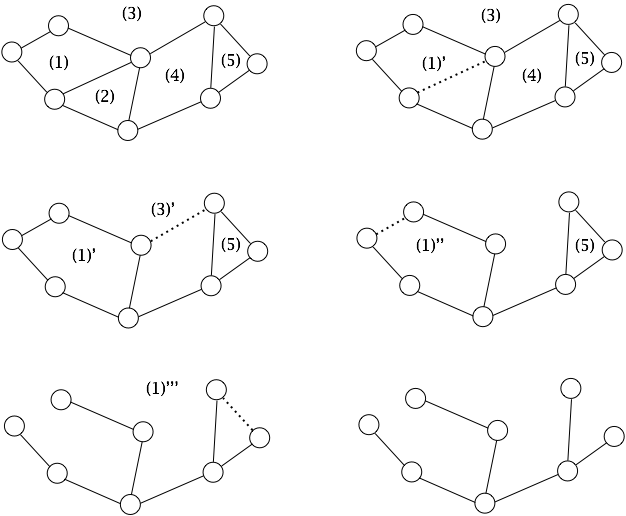
\includegraphics[scale=0.4]{FiguresGraph/planarStep1}
\caption{Illustrating Step 1: From top left to bottom right, each
  transformation preserves the invariant $\phi(n,e,f)$.  The first
  transformation removes the edge shared by faces (1) and (3),
  creating a new, merged, face (1)'.}
  \label{fig:planarStep1}
\end{center}
\end{figure}

\bigskip

{\bf The analysis}.
\begin{itemize}
\item
The graph remaining after an edge-removal is still planar---edges are
removed but never added---so we can continue the process.
\item
The process preserves the value of function $\phi$.  To wit, $n$ is
unchanged, while $e$ and $f$ are each reduced by $1$: $\phi(n,e,f) =
\phi(n,e-1,f-1)$.
\end{itemize}

\item[{\bf Step 2}.]
Iterate the following process of removing nodes from the tree produced
by Step 1, until onlu one node remains.

{\bf The action}.
Remove any leaf of the current tree, together with its incident edge.

Fig.~\ref{fig:planarStep2} illustrates the action of Step 2
for a tree  with $n=8$ nodes---hence, $e=7$ edges and $f=1$ face.
\begin{figure}[hbt]
\begin{center}
   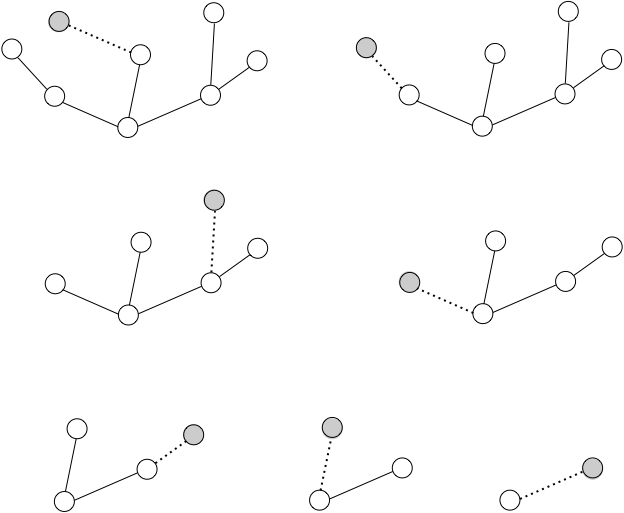
\includegraphics[scale=0.4]{FiguresGraph/planarStep2}
   \caption{Illustrating Step 2: We remove a sequence of leaves, each
     with its incident edge, until we reach a single node.  Again,
     $\phi$ remains invariant after each leaf-removal.}
  \label{fig:planarStep2}
\end{center}
\end{figure}

\bigskip

{\bf The analysis}.
The value of function $\phi$ remains unchanged by each leaf-removal.
To wit, $f$ is unchanged (it remains at $1$), while $n$ and $e$ are
each reduced by $1$: $\phi(n,e,f) = \phi(n-1,e-1,f)$
\end{description}

\noindent {\bf The cumulative analysis}.
\begin{itemize}
\item
Our process executes a number of steps exactly equal to the number of
edges of the graph $\g$ that we began with.  To wit, the edge-removal
Step removes $e-n$ edges, while the leaf-removal Step removes $n$
nodes.
\item
At the end of the process, $e=0$ and $n=f=1$, so that the residual
value of $\phi$ is $2$.  Because each action prescribed by the process
preserved the value of $\phi$, we know that $\phi$ has the value $2$
before each edge-removal and leaf-removal.
\end{itemize}
We conclude that, at the
start of the process,  $\phi(n,e,f)$ had the value $2$.  In other
words, $n-e+f = 2$.  This concludes the proof.  \qed


\subsection{Computing Chromatic Number}
\label{sec:Compute-Chromatic-No}

**HERE
**FIND REFERENCES

\cite{GareyJ79}
\cite{Karp72}

It is an {\sf NP}-complete problem to decide, given any fixed $k \geq
3$, whether a given graph $\g$ is $k$-colorable.

A simple argument shows that it is {\sf NP}-hard to find smallest
number of colors that provide a valid node-coloring of $\g$.

But one can exhibit ``greedy'' algorithms that give good results.



\section{$\oplus$ Pointers to Advanced Topics}
\label{sec:advanced-topics}

%**PROVIDE SOME REFERENCES

We conclude this chapter by mentioning a variety of topics that are
typically not covered---at least in depth---early in the curriculum,
but that are important enough that the reader should at least be aware
of them.  The topics we mention are motivated by virtually every
computational area that benefits from graph-theoretic models.  We have
tried to present each topic we touch on at a level of discourse that
will prepare the interested reader to delve more deeply into the
material, yet at a level of informality that will make the material
accessible to the more casual reader.  We thus strive for an intuitive
presentation that will not lead any reader astray.

The problem that we discuss in Section~\ref{sec:Relate-CS-Math-Probs}
illustrates how the {\em dynamic} models in the field of
algorithmics---``dynamic'' in the sense that they {\em do}
something---and the {\em structural} models provided by graph theory
can often provide beneficial illumination of one another.

Section~\ref{sec:graph-decompose} \index{graphs!graph separators}
\index{graphs!graph decomposition} focuses on the myriad computations
on graph that can be accomplished efficiently via recursive algorithms
that decompose, then reassemble, the graphs that they work on.

Section~\ref{sec:graph-evolve} \index{graphs!evolving graphs}
introduces the increasingly important topic of graphs whose structure
changes dynamically over time.  One timely instance of this dynamic
evolution is the connectivity graph of the Internet.

Section~\ref{sec:hypergraphs} \index{graphs!hypergraphs}
\index{hypergraphs} introduces {\it hypergraphs}, a generalization of
graphs that allows multi-entity relationships, in contrast to the
binary relationships mandated by graphs' two-element edges.
Hypergraph-based models find application in areas as diverse as:
\begin{itemize}
\item
{\it social networks:} Hyperedges can describe, e.g., collaboration
and collusion.
\item
{\it electronic networks:} Hyperedges can enable the design of
equi-potential nodes in voltage-driven technologies such as {\it
  VLSI}.
\item
{\it communication networks:} Hyperedges can model bus-oriented
communication.
\end{itemize}

\subsection{Hamiltonianicity in Weighted Graphs: the TSP}
\label{sec:TSP}
\index{Traveling Salesman Problem}

In Section~\ref{sec:Hamiltonian-unweighted}, we suggested how daunting
it is computationally to determine whether an unweighted graph admits
a Hamiltonian cycle.  There is an important, practically significant,
analogue of this problem for edge-weighted graphs, which has
traditionally been known as the {\it Traveling Salesman Problem}; we
shall use the modern abbreviation {\it TSP}.
\index{Traveling Salesman Problem}
\index{TSP: the Traveling Salesman Problem}
The TSP is a classical problem in Operations Research, whose familiar
name arises from the following story.
\index{Traveling Salesman Problem!origin of the name}

We consider a saleswoman who wants to make a call on all of her $n$
clients, who live in the $n$ cities, $C_1, C_2, \ldots, C_n$.  In
order to minimize the {\it cost} of her tour, she studies the
$\displaystyle {n \choose 2}$ real numbers $\{c_{i,j} \ | \ 1 \leq i,j
\leq n\}$, where each $c_{i,j}$ is the {\it cost} of traveling between
cities $C_i$ and $C_j$ (in either direction).  
\bigskip

\noindent \fbox{
\begin{minipage}{0.95\textwidth}
We are purposely vague about the meaning of the word ``cost'' here.
The costs represented by the unknowns $c_{i,j}$ could be intercity
driving distances or inter-region travel times or international
airfares.  Instances of the TSP can be formulated with {\em any}
notion of cost that can be represented by positive real numbers.

\smallskip

The importance of being vague is that, in particular, {\em none of
  these costs is assumed to obey any of the laws that one commonly
  associates with the distances we encounter in our daily lives}.  The
{\it triangle inequality} is a prime example of such a law.
\index{triangle inequality} Intuitively, this law insists that the
distance between any two cities is never decreased by placing an
intermediate stopover city between them.  It is a discretization of
the geometric postulate, {\em A straight line is the shortest distance
  between two points.}  Cost measures that obey the triangle
inequality are termed {\it Euclidean} \index{Euclidean distance
  measure} \index{Euclid} because the distances studied in Euclidean
geometry are assumed to obey this law.

\smallskip

Some people like to think of general intercity costs as
airfares---which clearly obey no immutable laws.)
\end{minipage}
}
\bigskip

The saleswoman's objective is to schedule the order of visiting her
clients' $n$ cities in the most economical way.  Formally, the
challenge of the TSP is to discover a minimum-cost tour of all $n$
cities.  Such a tour would be a cycle of the form
\[ C_{i_1} \ - \ C_{i_2} \ - \cdots - \ C_{i_n} \ - \ C_{i_1} \]
such that:
\begin{itemize}
\item
all $n$ cities appear in the tour precisely once;
\item
no tour has cost smaller than the cost
\[ c_{i_1,i_2} \ + \ c_{i_2, i_3} \ + \cdots + \  
c_{i_{n-1}, i_n} \ + \ c_{i_n, i_1} \]
of the indicated tour.
\end{itemize}
The main connection of the TSP to the current chapter is twofold.
\begin{enumerate}
\item
The TSP can be represented as a weighted analogue of the problem of
detecting Hamiltonian cycles.  Within this representation, the TSP's
$n$ cities are depicted as an instance of the complete graph $\k_n$,
and its intercity costs are real-number weights on the edges of
$\k_n$.  We describe this representation via the following informal,
but precise, encoding of a graph $\g$ as an instance of the TSP.
  \begin{itemize}
  \item
Each node of $\g$ becomes a ``city'' that must be visited.
  \item
For each pair of cities/nodes $A$ and $B$:
\[ \mbox{\sc cost}(A,B) \ = \ \left\{
\begin{array}{ccl}
1 & & \mbox{if there is an edge between $A$ and $B$ in $\g$} \\
\infty & & \mbox{if there is no edge between $A$ and $B$ in $\g$} \\
       & & \mbox{\small\sf (if the idea of ``infinite'' cost bothers
  you, then} \\
       & & \mbox{\small\sf make this some ridiculousy large number)}
\end{array}
\right.
\]
  \end{itemize}

\item
The TSP is computationally ``no easier'' than the
Hamiltonianicity-detection problem, in a very strong sense.  By
definition, the target of the TSP is a tour of minimum {\em overall
  cost}, as measured by the sum of the costs of the edges traversed in
the tour.  But, of course, {\em every} tour has some cost, according
to this measure.  The computational difficulty of the TSP is suggested
by the following result, which we state without proof.
\end{enumerate}

\begin{prop}[\cite{GareyJ79}]
\label{thm:Approx-TSP-NPC}
For any fixed positive constant $\kappa$, the problem of finding a
tour for an instance of the TSP that is within a factor of $\kappa$ of
minimal is an {\sf NP}-complete problem.
\end{prop}


The fact that TSP is a computationally complex problem is not very
surprising, because the TSP can be framed in a way that encompasses a
form of the Hamiltonianicity-detection problem.
What {\em is} surprising, though, is that if we restrict attention to
{\em Euclidean} instances of the TSP---i.e., instances whose ``costs''
measure Euclidean \index{Euclidean TSP problem} distances---say,
driving distances---then there exists a rather efficient algorithm
that solves such instances of the TSP {\em approximately} optimally,
\index{Traveling Salesman Problem!approximately optimal solution}
\index{TSP: the Traveling Salesman Problem!approximately optimal solution} 
in the sense of Proposition~\ref{thm:Approx-TSP-NPC}.  That is, there
exists a fixed constant $\kappa > 0$ such that, for each Euclidean
instance $\i$ of the TSP, if an {\em optimal}---i.e., {\em
  cost-minimal}---tour for instance $\i$ has cost $c^\star$, then the
cost of the tour discovered by the algorithm is no larger than $\kappa
\cdot c^\star$.  The algorithm that achieves this approximation is
named for its inventor, Nicos Christofides.
\index{Christofides, Nicos}

\ignore{*********
It corresponds to determine a minimal Hamiltonian cycle in a weighted
complete graphs $K_n$.  Obviously, $K_n$ is Hamiltonian (it exists
$n!$ such Hamiltonian paths), thus, the question here is to determine
the minimum one.

  Of course, she must go in every city and her objective is to
minimize the total distance done in the tour.  The only information
she has is the list of the cities and a map with all inter-cities
distances.  We assume a \textit{Euclidian distance} (for instance the
weights correspond to number of kilometers between two cities).  This
property means that the straight line is always the minimum distance,
or in other words that the distance between two vertices/cities is
larger if the path is going through any other vertex.
%More formally, the input of the problem is a weighted matrix with an infinite weight on the diagonal.
\bigskip
*****************}

\begin{prop}[\cite{Christofides76}]
There exists an algorithm for the Euclidean TSP that produces
approximately optimal tours, specifically, tours whose costs are no
greater than $1.5$ times the cost of an optimal tour.
\end{prop}

Proving this result is the domain of an algorithms text such as
\cite{CLRS}.  We remark only that the algorithm combines a number of
classical computational problems that admit efficient solutions:
minimum-weight spanning trees, preorder walks within trees, and
minimum-weight perfect matchings.

\ignore{***************
We construct an efficient solution for the Euclidean TSP, which is
known as {\it the Christofides algorithm}, \index{Christofides algorithm} 
after its inventor, Nicos Christofides.
\index{Christofides, Nicos}
\cite{Christofides76}

The following table, and Fig.~\ref{fig:perfectMatchingInitial}, depict
an instance of the Euclidian TSP with $n=7$ cities.
\[
\begin{array}{|c||c|c|c|c|c|c|c|}
\mbox{\bf City} & \multicolumn{6}{c}{\mbox{\bf Inter-City Costs}} \\
\hline
C_1 & 0 & c_{1,2} & c_{1,3} & c_{1,4} & c_{1,5} & c_{1,6} & c_{1,7} \\
\hline
C_2 & c_{2,1} & 0 & c_{2,3} & c_{2,4} & c_{2,5} & c_{2,6} & c_{2,7} \\
\hline
C_3 & c_{3,1} & c_{3,2} & 0 & c_{3,4} & c_{3,5} & c_{3,6} & c_{3,7} \\
\hline
C_4 & c_{4,1} & c_{4,2} & c_{4,3} & 0 & c_{4,5} & c_{4,6} & c_{4,7} \\
\hline
C_5 & c_{5,1} & c_{5,2} & c_{5,3} & c_{5,4} & 0 & c_{5,6} & c_{5,7} \\
\hline
C_6 & c_{6,1} & c_{6,2} & c_{6,3} & c_{6,4} & c_{6,5} & 0 & c_{6,7} \\
\hline
C_7 & c_{7,1} & c_{7,2} & c_{7,3} & c_{7,4} & c_{7,5} & c_{7,6} & 0 \\
\hline
\end{array}
\]


\begin{figure}[hbt]
\begin{center}
       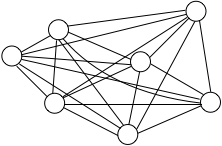
\includegraphics[scale=0.8]{FiguresGraph/christofides1}
\caption{An instance of the Euclidean TSP with $7$ cities, $C_1$,
  $C_2$, $C_3$, $C_4$, $C_5$, $C_6$, $C_7$, and intercity costs
  $\{c_{i,j} \ | \ 1 \leq i,j \leq 7\}$.}
              \label{fig:christofidesInitial}
\end{center}
\end{figure}


Let us construct a good solution (not \textit{too far} from the optimal) in polynomial time. 
Let us denote by $\omega_G$ the weight of graph G (i.e. the sum of the weights on its edges). 
The Chritofides algorithm proceeds in three steps. 
\bigskip

\textbf{Step 1.} Determine a minimal weight spanning tree $T^*$. 
%A spanning tree of G is a tree (connected graph with no cycle) with the same set of vertices as G. 
As we recalled in the preliminaries, a minimal weight spanning tree can be determined in polynomial time. 
\bigskip

$\omega_{T^*}$ is a lower bound of the value of the optimal tour $\omega_{H^*}$. 
Indeed, $H^*$ is a cycle, then, removing any edge in $H^*$ leads to a chain, which is a particular spanning tree.
As $T^*$ is the minimal spanning tree, we have:
$\omega_{T^*} \leq \omega_{H^*}$.

\begin{figure}[hbt]
\begin{center}
       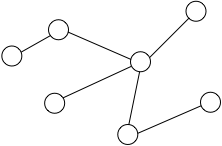
\includegraphics[scale=0.6]{FiguresGraph/christofides2}
       \caption{Construction of an optimal spanning Tree $T^*$.}
              \label{fig:christofidesSpanningTree}
\end{center}
\end{figure}


\textbf{Step 2.} Consider now the set $V_{odd}$ of the vertices of $T^*$ whose degrees are odd. 

We proved in the preliminary properties that the cardinality of $V_{odd}$ is even. 

Let us construct the perfect matching $C^*$ of minimum weight between the vertices in $V_{odd}$. 
Fig.~\ref{fig:AllPerfectMatchings} shows all possible perfect matchings on the previous example, the optimal one (with minimal weight) is represented in bold. 

Fig.~\ref{fig:christofidesPerfectMatching} illustrates the graph obtained by considering the edges of both $T^*$ and $C^*$. 
\begin{figure}[hbt]
\begin{center}
       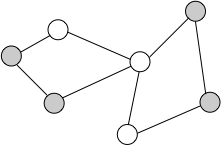
\includegraphics[scale=0.6]{FiguresGraph/christofides3}
       \caption{Adding the optimal perfect matching $C^*$ to the minimal spanning tree $T^*$.}
              \label{fig:christofidesPerfectMatching}
\end{center}
\end{figure}

Let us now determine a lower bound of the optimal tour $H^*$ (represented in Fig.~\ref{fig:perfectMatchingInitial}).

$2 \omega_{C^*}$ is a lower bound of the value of the optimal tour ($\omega_{C^*} \leq \frac{1}{2} \omega_{H^*}$). 
Indeed, consider first the perfect matching $C^*$.
As its vertices belong to $H^*$, $\omega_{C*}$ is lower than the piece of Hamiltonian tour contained between these vertices
because of the euclidian property (see Fig.~\ref{fig:perfectMatchingC*}).
Similarly for the \textit{complementary} perfect matching $C$ (Fig.~\ref{fig:perfectMatchingC}).  
Thus, the weight of the cycle formed by the concatenation of both perfect matchings is lower than the Hamiltonian tour $\omega_{C^* \bigcup C} \leq \omega_{H^*}$.
Moreover, as $C^*$ is the minimum perfect matching, we have $\omega_{C^*} \leq \omega_{C}$, this concludes the proof.


\begin{figure}[hbt]
\begin{center}
       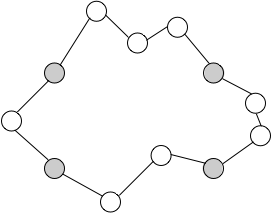
\includegraphics[scale=0.7]{FiguresGraph/perfectmatching1}
       \caption{An optimal Hamiltonian cycle $H^*$.}
              \label{fig:perfectMatchingInitial}
\end{center}
\end{figure}

\begin{figure}[hbt]
\begin{center}
       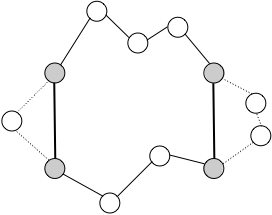
\includegraphics[scale=0.7]{FiguresGraph/perfectmatching2}
       \caption{Perfect matching $C^*$ between the vertices of odd degrees.}
              \label{fig:perfectMatchingC*}
\end{center}
\end{figure}

\begin{figure}[hbt]
\begin{center}
       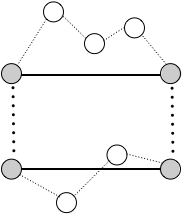
\includegraphics[scale=0.7]{FiguresGraph/perfectmatching3}
       \caption{Cycle $C^* \bigcup C$ (in dashed and bold).}
              \label{fig:perfectMatchingC}
\end{center}
\end{figure}

\bigskip

\textbf{Step 3.} 
All the vertices of $T^* \cup C^*$ have an even degree since we added an edge of $C^*$ to every odd degree vertices of $T^*$. 
We are now going to transform this graph by replacing iteratively the high degree vertices by shortcuts, which decreases the degree until reaching $2$. 

While it exists a vertex of degree greater than 4, we remove two of these consecutive edges and replace them by the opposite edge of this triangle 
without disconnecting the graph. There are $2k$ ways to remove $2$ edges and replace them by the triangle edge. Some of them disconnect the graph
and thus, must be avoided. 
Fig.~\ref{fig:christofidesFinalStep1} shows such a transformation on the previous example, 
Fig.~\ref{fig:christofidesFinalStep2} shows a valid transformation.

\begin{figure}[hbt]
\begin{center}
       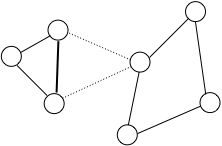
\includegraphics[scale=0.6]{FiguresGraph/christofides4}
       \caption{Reduction of the degree in $T^* \bigcup C^*$, disconnected solution.}
              \label{fig:christofidesFinalStep1}
\end{center}
\end{figure}

\begin{figure}[hbt]
\begin{center}
       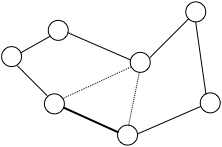
\includegraphics[scale=0.6]{FiguresGraph/christofides5}
       \caption{Reduction of the degree in $T^* \bigcup C^*$, connected solution.}
       \label{fig:christofidesFinalStep2}
\end{center}
\end{figure}

This process leads to a feasible tour. 
Such transformations do not increase the total weight.

Finally, 
as $\omega_{T^*} \leq \omega_{H^*}$ and $\omega_{C^*} \leq 1/2 \omega_{H^*}$,
we deduce that the value of such a tour is lower than $3/2 \omega_{H^*}$.
\qed
\end{proof}
*****************}


\subsection{Relating Computational and Mathematical Problems}
\label{sec:Relate-CS-Math-Probs}

This 

\ignore{*******************

\subsubsection{The Route Inspection/ Chinese Postman Problem}
\label{sec:chinesePostman}

**HERE

After solving the preceding ``pure'' version of the Eulerian-tour
problem---which seeks a tour of a graph which crosses each edge
precisely once---we discuss an extension of this problem which allows
us to augment a graph $\g$ by adding multiple edges between the same
two nodes.  (Terminologically, we thereby convert $\g$ to a {\it
  multi-graph} \index{multi-graph} \index{graphs!multi-graph}
consisting of nodes and {\it multi-edges}.) \index{multi-edge} Not
obviously, adding multi-edges can often convert a graph $\g$ that does
not admit an Eulerian cycle into a multi-graph that does admit an
Eulerian cycle.  The problem of finding the {\em smallest} such
augmentation of $\g$---i.e., of adding the fewest multi-edges---is
called the \index{Route Inspection Problem} {\it Route Inspection
  Problem}; it is also often called the {\it Chinese Postman Problem},
\index{Chinese Postman Problem} in honor of its inventor, the Chinese
mathematician Kwan Mei-Ko \index{Kwan Mei-Ko} \cite{Kwan60}.



This section is devoted to studying the {\it Route Inspection
  Problem}, \index{Route Inspection Problem} also known as the {\it
  Chinese Postman Problem}, \index{Chinese Postman Problem} in honor
of its inventor, the Chinese mathematician Kwan Mei-Ko \index{Kwan
  Mei-Ko} \cite{Kwan60}.  This problem seeks to add as few multi-edges
\index{graphs!multi-graph!multi-edge} as possible to a graph $\g$ in
order to render $\g$ Eulerian.  (A {\it multi-graph} is ``almost'' an
undirected graph.  It differs from a true graph because of the
possible presence of multiple multi-edges that connect the same two
nodes.)

**HERE


We know from Proposition~\ref{thm:eulerian-cycle} that if all of
$\g$'s nodes have even node-degrees, then---{\em and only then}---$\g$
admits an Eulerian cycle.  Therefore, in this case, {\em zero}
multi-edges need be added to $\g$ to render it Eulerian.  

Let us now present the more general problem of determining a cycle that contains all the edges in any graph, in particular when
there exist some odd vertices. From the previous section, we know that there is no Eulerian cycle in this case and thus, 
any feasible solution should duplicate some edges.
The problem is to duplicate the minimum.
This problem is known as the {\it chinese postman} and it is described below (in a french equivalent version).

A postman moved recently from Grenoble to a small village in the country side. 
He asked himself how to organize his daily tour by bike for distributing the letters in the shortest possible time. 
The director of the post office gives him the map and 
fortunately, the postman had some old souvenir of previous lectures in Graph Theory.  
The tour starts from the post office and of course, the postman has to go through every roads for distributing the letters before coming back
to his office.
The underlying graph is $G=(V,E)$ where $V$ is the (finite) set of cross points and $E$ is the set of the links between the cross roads
weighted by the distances.  

Fig.~\ref{fig:EulerianInitial} presents an example of the chinese postman problem. 
\begin{figure}[hbt]
\begin{center}
       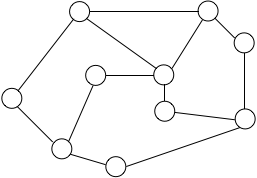
\includegraphics[scale=0.6]{FiguresGraph/EulerienInitial}
       \caption{An instance of the Chinese postman with $10$ cross-nodes.}
              \label{fig:EulerianInitial}
\end{center}
\end{figure}

\bigskip

This problem can be formulated mathematically in term of Eulerian
cycles.  Intuitively, the basic idea is to duplicate some edges that
are carefully chosen in order to use the previous construction of an
Eulerian tour of Section~\ref{sec:EulerianCycle} that will help the
postman to determine the optimal tour (of minimal length) using some
simple mathematical properties.
\bigskip

First, we know that there is an even number of odd vertices.
Considering the previous instance of the postman problem, there are $4$ such vertices (represented in grey in Fig.~\ref{fig:EulerianVodd}).

\begin{figure}[hbt]
\begin{center}
       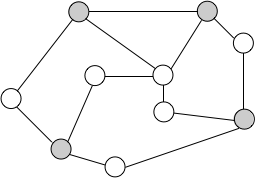
\includegraphics[scale=0.6]{FiguresGraph/EulerienVodd}
       \caption{The $4$ vertices with an odd degree in the previous instance.}
              \label{fig:EulerianVodd}
\end{center}
\end{figure}
\bigskip

As there exists a path between any pair of vertices of odd degree in $V_{odd}$,
we consider the complete graph whose vertices are the odd degree vertices weighting the edges with the shortest paths (denoted by $K_{odd}$).
As we mentioned in the preliminary properties, computing the shortest paths is a classical problem, which can be solved in polynomial time. 

\begin{figure}[hbt]
\begin{center}
       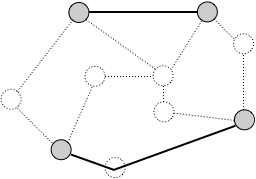
\includegraphics[scale=0.6]{FiguresGraph/EulerienPerfectMatching}
       \caption{The minimum weight perfect matching labelled by the shortest distances between the vertices of $V_{odd}$.}
              \label{fig:Eulerianperfectmatching}
\end{center}
\end{figure}
\bigskip

Then, it is possible to do the correspondence between the optimal solution of the postman problem and a perfect matching of minimal weight in $K_{odd}$
%Recall that a matching is a set of edges without common vertices. It is perfect if it has the maximum number of edges. 
by duplicating the edges of the minimal perfect matching.

\begin{figure}[hbt]
\begin{center}
       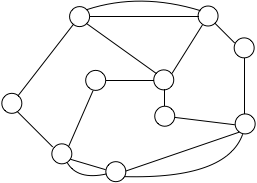
\includegraphics[scale=0.6]{FiguresGraph/EulerienFinal}
       \caption{Final step: adding the edges of the minimum perfect matching.}
              \label{fig:EulerianFinal}
\end{center}
\end{figure}

The main steps of the algorithm for determining the optimal tour are the following:

\begin{itemize}
\item Consider the complete graph with the odd vertices and compute its weight by the shortest paths.
Compute a perfect matching of minimal weight between these vertices. 
\item Duplicate all the edges along the paths of this matching.
\item Determine an Eulerian tour in this new graph with even degrees.
\end{itemize}

The optimality of this algorithm comes from the fact that the duplicated edges are the minimum possible ones.
% This is straightforward for two odd vertices.
Finally, all the vertices of the new graph are even since the degree of the odd vertices in $G$ is augmented by $1$
(extremities of the paths) and the other even vertices which are intermediate vertices of the paths remain even. 

\medskip

This short discussion is a good segu\'{e} to the material in the next
section, which leds valuable perspective on our brief study of
Hamiltonian paths and cycles---and, indeed, on the computational
implications of that work.
*************************}

\subsection{Graph Decomposition}
\label{sec:graph-decompose}
\index{graphs!decomposition}
\index{graphs!bisector}
\index{graphs!separator}

The reader will certainly have noted that some ``named'' graphs are,
intuitively, more tightly interconnected than others.  From a purely
intellectual vantage point, it would be of interest to be able to
quantify the tightness of interconnection.  Among the various measures
that have been proposed, one stands out for its myriad algorithmic
implications: the notion of {\it graph separator}.  In fact, this
notion appears in the literature in several flavors.  An $n$-node,
$e$-edge graph $\g$ has:
\begin{itemize}
\item
an {\it $\alpha$-edge separator} of size $k$, 
\index{graphs!$\alpha$-edge separator of size $k$} where $\alpha$ is a
real number with $\alpha \leq 1/2$ and $k$ is an integer with $k < n$,
precisely if:

\smallskip

one can partition $\g$ into two disjoint (not-necessarily connected)
subgraphs, each having $\leq \alpha n$ nodes, by removing $\leq k$
edges from $\g$.

\item
a {\it $\alpha$-node separator} of size $\ell$,
\index{graphs!$\alpha$-node separator of size $\ell$}
where $\alpha$ is a real number with $\alpha \leq 1/2$ and $\ell$ is
an integer with $k < e$, precisely if:

\smallskip

one can partition $\g$ into two disjoint (not-necessarily connected)
subgraphs, each having $\leq \alpha n$ nodes, by removing $\leq \ell$
nodes from $\g$.
\end{itemize}
We replace the term ``separator'' with the term {\em ``bisector''} 
\index{graphs!edge bisector} \index{graphs!node bisector}
if both subgraphs after a separation operation have $\leq \lfloor
\frac{1}{2} n \rfloor$ nodes.

\medskip

Commonalities and differences in inherent separator sizes are often
not visually obvious.  For illustration, referring to the ``named''
graphs of Section~\ref{sec:graphs-important-families}:
\begin{itemize}
\item
It is certainly obvious that cycles are easier to bisect than cliques,
as measured by either edge or node bisectors.
\item
It is far less clear that de Bruijn networks and hypercubes are
roughly equal in ease to bisect, as measured by node bisectors.
\end{itemize}
But similar separation behavior has very important algorithmic
consequences.  For instance, the closeness in separation
characteristics between de Bruijn networks and hypercubes manifests
itself in a large range of algorithmic applications.  The range of
such applications is hinted at by sources that study the algorithmics
of laying out VLSI circuits (see, e.g., \cite{Leiserson85}) and
sources that study the ability of a network's interconnections to host
a range of communication patterns that enable efficient parallel
computation and communication (see, e.g.,
\cite{AnnexsteinBR90,Leiserson85,Ullman84}).


\medskip

There is a large literature that develops the algorithmics of finding
small separators for significant families of graphs.  An early star in
the firmament of such studies is the discovery in \cite{LiptonT79} of
a $1/3$-node separator of size $\sqrt{8n}$ for $n$-node planar graphs.
The dual problem of finding lower bounds on the sizes of graph
separators is a bit sparser but, of course, no less significant.  The
reader can find a comprehensive exposition on the theory of graph
separators in \cite{RosenbergH01}, including both the mathematics that
yields lower bounds on separator sizes and the algorithmics that
yields upper bounds.


\subsection{Graphs with Evolving Structure}
\label{sec:graph-evolve}
\index{graphs!with evolving structure}

Classical problems in the area of graph algorithms will discuss
graphs, especially trees, whose structures evolve over time.  Such
evolution is observed, e.g., in the study of ``classical'' algorithmic
problems such as {\it Minimum Spanning Tree} and {\it Branch and
  Bound}; see, e.g., \cite{CLRS}.  What is certain to be more exciting
to the reader, though, are the ``modern'' topics where one encounters
graphs with evolving structure, such as {\it social networks} and {\it
  inter-networks} (e.g., the {\it Internet of Things}).

For ``classical'' topics, as exemplified by the two we have mentioned,
the mathematics covered in this chapter will provide the reader with
the background necessary to deal with graph evolution.  Indeed, this
evolution emerges as an inevitable concomitant of the algorithmics
that is superimposed upon the traditional structures of graph theory:
the challenge to the reader is to assimilate new algorithmic notions,
not new mathematics.

\index{graphs!with evolving structure!social networks}
\index{graphs!with evolving structure!inter-networks}
In contrast, the ``modern'' topics we have mentioned do require the
reader's assimilating new mathematics.  Dealing successfully with the
algorithmic issues that arise with social networks and inter-networks
requires the reader to understand the structures of the evolving
graph-oriented systems and how evolution changes these structures.
Among the interesting (and valuable) mathematical questions one can
pose is: When a new node applies to join an evolving network, which
node in the network is the best one to connect to, in order to best
facilitate one's interactions or influence within the community.  The
latter topic leads, e.g., to the study of {\em power-law} networks.
\index{graphs!with evolving structure!social networks!power-law networks}
\index{graphs!with power-law degreegrowth patterns}
\bigskip

\noindent \fbox{
\begin{minipage}{0.95\textwidth}
An evolving network is said to {\it obey a power law} if there exists
a real number $\gamma >0$ such that, for sufficiently large values of
the integer parameter $k$, the fraction of nodes in the network having
degree $k$ is proportional to $k^{-\gamma}$.
\end{minipage}
}
\bigskip

Little of the abstract work on power-law networks would likely be
studied in depth in any early course; indeed, the structure of these
networks is not yet well understood even in advanced settings.
Attempts to understand power laws with rigor have given rise to a
number of competing, rather sophisticated, abstract models---see,
e.g., \cite{AielloCL00,BarabasiA99,Bollobas85,ChenCGJSW}---and
numerous studies have attempted to understand the specific situations
wherein the abstract models reflect reality more or less
faithfully---see, e.g.,
\cite{BuT02,FaloutsosFF99,JaiswalRT04,TangmunarunkitGJSW02,ZeguraCD97}.


\subsection{Hypergraphs}
\label{sec:hypergraphs}
\index{graphs!generalization to hypergraphs}
\index{hypergraphs}

A large variety of modern computing-related topics benefit from the
structure inherent in graph-theoretic models but do not comfortably
conform to the {\em binary} relationships imposed by graphs' having
{\em two} nodes per edge.  A model that retains the structure of
graph-theoretic models without the binary constraint is the
generalization of graphs called {\em hypergraphs}.  A hypergraph has
nodes that play exactly the same role as with graphs, but in place of
a graph's binary edges, a hypergraph has {\em hyperedges}, each being
a set of nodes whose size is not restricted to $2$.  A rather general
treatment of hypergraphs can be found in the comprehensive
graph-theory text \cite{Berge73}; a specialized article that focuses
on some of the topics of this chapter, such as node-coloring, is
\cite{Lovasz73}.  Because of their inherent complexity, hypergraphs as
graph-theoretic objects are usually relegated to advanced courses.
However, the literature contains many studies of hypergraphs that are
``fine-tuned'' for specific computing-related application areas, and
many of these should be accessible without extensive mathematical
background.  Sample  computing-related application areas that benefit
from hypergraph-oriented models include the following.
\begin{itemize}
\item
Bus-connected parallel communication has been part of digital computer
\index{hypergraphs!modeling bus-connected communication} design since
its earliest days.  The informal picture of such a system is that
there are communication channels that multiple agents can retrieve
message from and post messages to.  In hypergraph-oriented terms: the
nodes/communicating agents aggregate into groups/hyperedges.  Each
group's agents share ``read/write'' access to a specific channel.  A
spcialized genre of hypergraph that was invented to study the
described scenario is the {\it interval hypergraph}
\index{hypergraphs!interval hyergraphs} model developed in
\cite{Rosenberg89a}.

\item
Modern electronic circuits are implemented using integrated circuit
\index{hypergraphs!modeling integrated circuits} technology,
specifically, {\em VLSI: Very Large Scale Integrated circuitry}; see,
e.g., \cite{Mead-Conway}.  These technologies tend to be
voltage-driven, rather than current-driven.  Accordingly, much of the
attention when designing circuits centers on the coordination of
equi-potential points in a network, rather than on point-to-point
transmission of signals.  Hypercubes are tailor-made for such
technologies.  A crucially important issue that arises because of the
design strengths and weaknesses of  VLSI technology is {\it fault
  tolerance}---how to cope with the inevitable faulty transistors in
massive VLSI systems.  Even mathematically quite-accessible ideas can
provide provocative ideas about this important topics; see, e.g.,
\cite{Rosenberg85a}

\item
Social networks have become so prevalent in society that no one will
be surprised to learn that many approaches to modeling the networks'
interconnectivity have been studied.  In
Section~\ref{sec:graph-evolve}, we discussed an interconnectivity
model based on evolving graphs and clustering within such graphs.
More recently, hypergraph-based models
\index{hypergraphs!modeling interconnectivity in social networks}
have also been proposed; see, e.g., \cite{Amatoetal17,LiuBV10}.
\end{itemize}





%chapter
%*********REVISED 01-30-18

%%%%%%%%%%%%%%%%%%%%%%%%%%%%%%%%%

%version of 02-01-18

\chapter{ASYMPTOTICS}
\label{sec:asymptotics}

{\em Asymptotics} can be viewed as a language and a system of
reasoning that allow one to talk in a {\em qualitative} voice about
{\em quantitative} topics.  We thereby generalize to arbitrary growth
functions terms such as ``linear'', ``quadratic'', ``exponential'',
and ``logarithmic''.

Such a language and system are indispensable if one needs to reason
about computational topics over a range of situations, such as a range
(``all existing''?)  computer architectures and software systems.  As
two simple examples: (1) Carry-ripple adders perform additions in time
linear in the lengths $n$ of the summands (measured in number of bits)
no matter what these lengths are. (2) Comparison-based sorting
algorithms can sort lists of $n$ keys in time proportional to $n \log
n$, but no faster---where the base of the logarithm depends on the
characteristics of the computing platform.  More precise versions of
the preceding statements require specication of the number $n$ and
other details, possibly down to the clock speeds of the host
computer's circuitry.

\section{The language of asymptotics}

The language of asymptotics, which has its origins in the field of
Number Theory in the late 19th century, builds on the following
terminology, which is likely what one would cover in an early
undergraduate course.  More advanced aspects of the language would
likely by beyond the needs of most students of computing, aside from
specialists in advanced courses.  The basics of the language build on
three primitive notations and notions.  Standard sources, such as any
text on algorithm design and analysis, flesh out the following ideas.
\begin{itemize}
\item
{\em The big-O notation}.
%
The assertion $f(x) = O(g(x))$ says, intuitively, that the function
$f$ grows no faster than function $g$.  It is, thus, the asymptotic
analogue of ``less than''.

Formally:
$f(x) = O(g(x))$

means

$(\exists c >0)(\exists x^{\#})(\forall x > x^{\#})
[f(x) \leq c \cdot g(x)]$

\item
{\em The big-$\Omega$ notation}.
%
The assertion $f(x) = \Omega(g(x))$ says, intuitively, that the
function $f$ grows at least as fast as function $g$.  It is, thus, the
asymptotic analogue of ``greater than''.

Formally:
$f(x) = \Omega(g(x))$

means

$(\exists c >0)(\exists x^{\#})(\forall x > x^{\#})
[f(x) \geq c \cdot  g(x)]$ \\

\item
{\em The big-$\Theta$ notation}.
%
The assertion $f(n) = \Theta(g(n))$ says, intuitively, that the
function $f$ grows at the same rate as does function $g$.  It is,
thus, the asymptotic analogue of ``equal to''.

Formally:
$f(x) = \Theta(g(x))$

means

$(\exists c_1 >0)(\exists c_2 >0)(\exists x^{\#})(\forall x > x^{\#})
[c_1 \cdot g(x) \leq f(x) \leq c_2 \cdot  g(x)]$
\end{itemize}
One renders the preceding intuitive explanations precise by pointing
out that the three specifies relations ($a$) take hold {\em
  eventually}, i.e., only for large arguments to the functions $f$ and
$g$, and ($b$) hold up to an unspecified constant of proportionality.

\ignore{*********
\subsubsection{Getting formal}

{\small\sf Big-$O$, Big-$\Omega$, and Big-$\Theta$ notation}.%
It is convenient to have terminology and a notation that allows us to
talk about the rate of growth of one function as measured by the rate
of growth of another.  We are interested in the exact growth rate, as
well as upper and lower bounds on the growth rate.  We do have
appropriate such language for certain rates of growth.  We can talk,
for instance, about a linear growth rate or a quadratic rate or an
exponential rate, to name just a few---and we get the desired bounds
using the prefixes ``sub'' or ``super,'' as in ``subexponential'' and
``superlinear''---but our repertoire of such terms is quite limited.
Mathematicians working in the theory of numbers in the late nineteenth
century established a notation that gives us an unlimited repertoire
of descriptors for growth rates, via what has come to be called the
big-$O$, big-$\Omega$, and big-$\Theta$ notations, which are
collectively sometimes called {\em asymptotic notation}.\index{asymptotic notation}
*******}

\section{The ``uncertainties'' in asymptotic relationships}

The formal definitions of all three of our asymptotic relationships
are bracketed by two important quantifiers:
\[ ``(\exists c >0)'' \ \ \ \mbox{ and } 
 ``(\forall x > x^{\#})''.
\]
The former, {\em uncertain-size} quantifier, asserts that asymptotic
notions describe functional behavior ``in the large''.  Thus, in
common with more common qualitative descriptors of quantitative growth
such as linear, quadratic, cubic, quartic, exponential, logarithmic,
etc., asymptotic relationships give no infomation about constants of
proportionality.  {\em We are not saying that constant factors do not
  matter!  We are, rather, saying that we want to discuss growth
  patterns \underline{in the large}.}

The latter, {\em uncertain-time} quantifier asserts that asymptotic
relationships between functions are promised to hold only
``eventually'', i.e., ``for sufficiently large values of the argument
$x$''.  Therefore, in particular, asymptotic notions cannot be
employed to discuss or analyze quantities that can never grow beyond a
fixed finite value.  The fact that all instances of a quantity
throughout history have been below $N$ is immaterial, as long as it is
conceivable that an instance larger than $N$ could appear at some time
in the future.

These quantifiers in particular distinguishes claims of asymptotic
relationship from the more familiar definite inequalities such as
``$f(x) \leq g(x)$'' or $f(x) \geq 7 \cdot g(x)$.  In fact, it is
often easier to think about our three asymptotic bounding assertions
as establishing {\em envelopes} for $f(x)$:
\begin{itemize}
\item
Say that $f(x) = O(g(x))$.  If one draws the graphs of the functions
$f(x)$ and $c \cdot g(x)$, then as one traces the graphs with
increasing values of $x$, one eventually reaches a point $x^{\#}$
beyond which the graph of $f(x)$ never enters the territory {\em
  above} the graph of $c \cdot g(x)$.
\item
Say that $f(x) = \Omega(g(x))$.  This situation is the up-down mirror
image of the preceding one: just replace the highlighted ``{\em
above}'' with ``{\em below}.''
\item
Say that $f(x) = \Theta(g(x))$.  We now have a two-sided envelope:
beyond $x^{\#}$, the graph of $f(x)$ never enters the territory {\em
  above} the graph of $c_1 \cdot g(x)$ and never enters the territory
{\em below} the graph of $c_2 \cdot g(x)$.
\end{itemize}
In addition to allowing one to make familiar growth-rate comparisons
such as ``$n^{14} = O(n^{15})$'' and ``$1.001^n = \Omega(n^{1000})$,''
we can now also make assertions such as ``$\sin x = \Theta(1)$,''
which are much clumsier to explain in words.


\noindent {\bf Beyond the big letters.}
%
There are ``small''-letter analogues of the preceding ``big''-letter
asymptotic notations, but they are only rarely encountered in
discourse about real computations (although they do arise in the
analysis of algorithms).

\section{Inescapable complications}

The story we have told thus far is covered in many sources and
courses.  Two complications to the story are covered less faithfully,
although lacking them, one cannot perform cogent asymptotic
reasoning.  Both complications involve the notion of {\em uniformity}.

\noindent
{\bf 1.}
{\em Multiple functions}.
%
Say that we have four functions, $f, g, h, k$, and we know that both
\[ f(n) = O(g(n)) \ \ \mbox{ and } \ \ h(n) = O(k(n)) \]
It is intuitive that
\[ f(n) + h(n) = O(g(n) + k(n)) \]
--- but is it true?

In short, the answer is YES, but verifying that requires a bit of
subtlety, because, absent hitherto undisclosed information, the
proportionality constants $c_{f,g}$ and $N_{f,g}$ that witness the
big-$O$ relationship between functions $f$ and $g$ have no connection
with the constants, $c_{h,k}, N_{h,k}$ that witness the analogous
relationship between functions $h$ and $k$.  Therefore, in order to
verify the posited relationship between functions $f + h$ and $g + k$,
one much find witnessing constants $c_{f+h, g+k}$ and $N_{f+h,g+k}$.
Of course, this task requires only elementary reasoning and
manipulation --- but it must be done!

{\bf 2.}
{\em Multivariate functions}.
%
Finally, we discuss the scenario that almost automatically accompanies
the transition from a focus on sequential, single-agent computing to a
focus on PDC.  Within this broadened context, most functions that
describe a system have one or more variables that describe the
computing system --- its number of processors or of agents or the
sizes of its memory modules or the communication-radii of its
transponders or \ldots, in addition to the one or more variables that
describe the data that the system is processing.  Within such
scenarios, every assertion of an asymptotic relationship, of the form
\[ f(\vec{m}; \vec{n}) = O(g(\vec{m}; \vec{n})) \]
must explicitly specify the following information:
\begin{itemize}
\item
which variables can grow without bound;
\item
among such unbounded variables, which participate in the posited
asymptotic relation;
\item
for each participating unbounded variable $x$, what are the constants
$c_x$ and $N_x$ that witness the posited asymptotic relationship(s).
\end{itemize}

Clearly the complexity of cogent asymptotic reasoning --- hence also
the complexity of teaching about such reasoning --- gets much more
complicated in the multivariate settings engendered by PDC.  But, the
benefits of being able to reason qualitatively about the quantitative
aspects of computing increase at least commensurately!

%chapter
%*********REVISED 01-30-18


%%%%%%%%%%%%%%%%%%%%%%%%%%%%%%%%%

%version of 01-30-18

\chapter{PROBABILITY AND STATISTICS}
\label{ch:prob-stat}

Elements of probability theory and statistics infuse every area of
computing.  The practicality of many algorithms that are
experientially the most efficient for their target tasks depend on the
{\em distribution} of inputs in ``real" situations.  Design
methodologies for crucial complex circuits must acknowledge the {\em
  mean times to failure} of the critical components of the circuits.
Sophisticated searching algorithms must take into account the relative
{\em likelihoods} of finding one's goal in the various optional search
directions.  Analyzing and understanding large corpora of data
requires a variety of methodologies that build on the concepts of {\em
  clustering} and/or {\em decomposition}.

A student needs at least an introduction to the foundations of
probability and statistics to even understand, all the moreso to
master, the terms highlighted in the preceding paragraph.  We outline
many of the key concepts that a student must be exposed to in the
following subsections.


\section{The Elements of Combinatorial Probability}

Perhaps the easiest and most engaging way to introduce ``probability
via counting" is by calculating the comparative likelihoods of various
deals in $5$-card poker and of various rolls of a pair of dice.  The
arithmetic required for this discussion is elementary and the
``application" to gambling of interest even to non-gamblers: ``Why is
such a deal in poker (say, a straight) worth more than another (say,
three of a kind)?"  One can also introduce in this setting concepts
such as randomness, bias, etc., that are so important in the design of
experiments and the analysis of their outcomes.

\section{Toward a Basic Understanding of Statistics}

Most students whose interest tend to the empirical will likely ``do"
statistics with the aid of apps, rather than by explicitly writing
programs that perform the required calculations.  That said, all
students should understand the crucial notion of {\em random variable}
and should be conversant with the most common statistical
distributions.  ``Conversant" in this context should include complete
understandings of the (low-numbered) moments of {\em at least} the
{\em uniform} and {\em exponential} distributions.  They should know
how to compute, say, the means and variances of various distributions
— and, most importantly, they should {\em understand} the sense in
which the variance of a distribution give {\em important} information
that is not available from the mean.  All of this is prerequisite to
rigor in experimentation.

\subsubsection{The Elements of Empirical Reasoning}

Empirical reasoning does not convey the certitude that formal
reasoning does.  Students should understand how to craft experiments
in a way that collects the ``right'' data.  The should then be
able---perhaps just with statistical packages---to interpret the
results they collect and to understand what conclusions are
justifiable.  {\em It is essential that all students understand the                  
  ditinction between {\em positive correlation} and {\em causation}!}
(Most of the public would seem to flunk that test.)

In order to satisfy the preceding demands, students should understand
enough about statistics---including definitions and meanings related
to distributions and their moments---to understand what conclusions
can be made based on experimental results, and to understand how to
describe conclusions in a way that is supported by the statistics.

\section{Beyond the Basics}

As students are introduced to modern topics within computing, whether
at the level of a Computing Literacy course or a post-core technical
course, they will have to master a variety of more specialized topics
that combine pieces of the elements we have discussed in this essay.
While these topics are beyond the level of generality aimed at in this
essay, some may be appropriate prerequisites to programs that have
some specialized foci.
\begin{itemize}
\item
Issues relating to {\em clustering} find application in applicatios as
diverse as: {\em linear-algebraic computations}, {\em data mining},
{\em design and layout of digital circuitry}.

\item
Issues building on {\em graph separation/decomposition} are
encountered when studying: {\em linear-algebraic computing}, {\em
  fault-tolerant design}, {\em load balancing}.

\item
Many issues relating to {\em fault/failure tolerance} and {\em data
  analytics} benefit from study using {\em random walks} (at least in
one dimension).

\item
Many useful ideas regarding the {\em encoding and manipulation of
  data} can be gleaned from the elements of {\em information theory}
and {\em computer arithmetic}.
\end{itemize}
The preceding list is really endless.  Hopefully readers will be
inspired by our few examples to compile a longer version that is
appropriate for their particular environments.

%chapter
%*********REVISED 01-30-18

%%%%%%%%%%%%%%%%%%%%%%%%%%%%%%%%%

%\addcontentsline{toc}{chapter}{V \ Sample Exercises}
%\input{Exercises}%part

\backmatter

%version of 01-29-19

\begin{thebibliography}{999}

%A

\bibitem{AnnexsteinBR90}
F.~Annexstein, M.~Baumslag, A.L.~Rosenberg (1990):
Group action graphs and parallel architectures.
{\it SIAM J.~Comput.~19}, 544--569.

%B

\bibitem{Basin63}
S.L.~Basin (1963): The Fibonacci Sequence as it appears in nature.
{\it Fibonacci Quart.~1}, 53--57.

\bibitem{Bell86}
E.T.~Bell (1986):
{\it Men of Mathematics}.
Simon and Schuster, New York.

\bibitem{Berge73}
C.~Berge (1973):
{\it Graphs and Hypergraphs}.
North-Holland, Amsterdam.

\bibitem{BermondP89}
J.-C.~Bermond, C.~Peyrat (1989):
The de Bruijn and Kautz networks: a competitor for the hypercube?
In {\it Hypercube and Distributed Computers} (F.~Andre and
J.P.~Verjus, eds.)  North-Holland, Amsterdam, 279--293.

\bibitem{Bernstein05}
F.~Bernstein (1905): Untersuchungen aus der Mengenlehre. {\it
Math.~Ann.~61}, 117--155.

\bibitem{Birkhoff-MacLane53}
G.~Birkhoff and S.~Mac Lane (1953): {\it A Survey of Modern Algebra},
Macmillan, New York.

\bibitem{Bishop67}
E.~Bishop (1967): {\it Foundations of Constructive Analysis},
McGraw Hill, New York.

\bibitem{BooneCL73}
W.W.~Boone, F.B.~Cannonito, R.C.~Lyndon (1973):
{\it Word Problems: Decision Problem in Group Theory}, North-Holland,
Amsterdam.


%C

\bibitem{Cantor74}
G.~Cantor (1874): \"{U}ber eine Eigenschaft des Inbegriffes aller
reellen algebraischen Zahlen.  {\it J.~Reine und Angew.~Math.~77},
258--262.

\bibitem{Cantor78}
G.~Cantor (1878): Ein Beitrag zur Begr\"{u}ndung der transfiniter
Mengenlehre.  {\it J.~Reine Angew.~Math.~84}, 242--258.

\bibitem{Cantor87}
G.~Cantor (1887): Mitteilungen zur Lehre vom Transfiniten.
{\it Zeitschrift f\"{u} Philosophie und Philosophische Kritik 91}
81-–125.

\bibitem{Cauchy21}
A.L.~Cauchy (1821): {\it Cours d'analyse de l'\'{E}cole Royale
Polytechnique, 1\`{e}re partie: Analyse alg\'{e}brique}.
l'Imprimerie Royale, Paris.  Reprinted: Wissenschaftliche
Buchgesellschaft, Darmstadt, 1968.

\bibitem{ChartrandK69}
G.~Chartrand, S.F.~Kapoor (1969):
The cube of every connected graph is 1-hamiltonian.
{\it J.~Research of the National Bureau of Standards, 73B(1)}.  DOI:
10.6028/jres.073B.007

\bibitem{Christofides76}
N.~Christofides (1976):
Worst-case analysis of a new heuristic for the travelling salesman
problem.  Report 388, Graduate School of Industrial Administration,
Carnegie-Mellon Univ.

\bibitem{Cook71}
S.A.~Cook (1971): The complexity of theorem-proving procedures.  {\it
  ACM Symp.~on Theory of Computing}, 151--158.

\bibitem{CLRS}
T.H.~Cormen, C.E.~Leiserson, R.L.~Rivest, C.~Stein (2001):
{\it Introduction to Algorithms (2nd ed.)}.
MIT Press, Cambridge, MA.

\bibitem{Curry34}
H.B.~Curry (1934): Some properties of equality and implication in
combinatory logic.  {\it Annals of Mathematics, 35}, 849--850.

\bibitem{CurryFC58}
H.B.~Curry, R.~Feys, W.~Craig (1958):
{\it Combinatory Logic.  Studies in logic and the foundations of
mathematics}.  North-Holland, Amsterdam.

%D

\bibitem{Davis58}
M.~Davis (1958):
{\it Computability and Unsolvability.}
McGraw-Hill, New York.

\bibitem{Deiser2010}
O.~Deiser (2010): Einf\"{u}hrung in die Mengenlehre – Die Mengenlehre
Georg Cantors und ihre Axiomatisierung durch Ernst Zermelo (3rd,
corrected ed.), Berlin/Heidelberg: Springer, pp. 71, 501,
doi:10.1007/978-3-642-01445-1, ISBN 978-3-642-01444-4.


%F

\bibitem{Fleischner74}
H.~Fleischner (1974):
The square of every two-connected graph is hamiltonian.
{\it J.~Combinatorics Theory (B) 16}, 29--34.

\bibitem{Fubini}
G.~Fubini (1907): Sugli integrali multipli.
{\it Rom.~Acc.~L.~Rend.~(5), 16(1)}, pp.~608–614.  In {\it zbMATH
  38.0343.02}.  Reprinted in
G.~Fubini (1958): {\it Opere scelte, 2}, Cremonese, pp. 243–249.

\bibitem{FueterP23}
R.~Fueter and G.~P\'{o}lya (1923):
Rationale Abz\"{a}hlung der Gitterpunkte.  {\it
Vierteljschr.~Naturforsch.~Ges.~Z\"{u}rich 58}, 380--386.

%G

\bibitem{GareyJ79}
M.R.~Garey and D.S.~Johnson (1979):
{\it Computers and Intractability}.
W.H.~Freeman and Co., San Francisco.

\bibitem{Goedel31}
K.~G\"{o}del (1931): \"{U}ber Formal Unentscheidbare S\"{a}tze der
Principia Mathematica und Verwandter Systeme, I.  {\it Monatshefte
f\"{u}r Mathematik u.~Physik 38}, 173--198.


%H

\bibitem{Halmos60}
P.R.~Halmos (1960):
{\it Naive Set Theory}.
D.~Van Nostrand, New York.

\bibitem{Hazewinkel}
M.~Hazewinkel, ed. (2001): %[1994],
Vi\`{e}te theorem.  In {\it Encyclopedia of Mathematics}.
Springer Science+Business Media B.V./Kluwer Academic Publishers,
ISBN 978-1-55608-010-4.

\bibitem{Horner}
W.G.~Horner (1819): 
A new method of solving numerical equations of all orders, by
continuous approximation. {\it Philosophical Transactions. Royal
Society of London}, 308-–335.

%I


%J

\bibitem{JohnssonH1989}
S.L.~Johnsson, C.T.~Ho (1989):
Optimum broadcasting and personalized communication in hypercubes.
{\it IEEE Trans.~Computers 38}, 1249--1268.


%K

\bibitem{Karp72}
R.M.~Karp (1972): Reducibility among combinatorial problems.  In {\it
Complexity of Computer Computations} (R.E.~Miller and J.W.~Thatcher,
eds.)  Plenum Press, NY, pp.~85--103.

\bibitem{Kleene36}
S.C.~Kleene (1936): General recursive functions of natural numbers.
{\it Math.~Annalen 112}, 727--742.

\bibitem{Kleene52}
S.C.~Kleene (1952):
{\it Introduction to Metamathematics.}
D.~Van Nostrand, Princeton, NJ.

\bibitem{Konig36}
D.~K\"onig (1936):
{\it Theorie der endlichen und unendlichen Graphen.}  Lipzig: Akad.~Verlag.

\bibitem{Kuhn55}
H.W.~Kuhn (1955): The Hungarian method for the assignment problem.
{\it Naval Research Logistics Quarterly 2}, 83-–97.

\bibitem{Kwan60}
Kwan, Mei-Ko (1960): Graphic programming using odd or even points.
{\it Acta Mathematica Sinica, 10} (in Chinese), 263--266.  Translated
into English in {\it Chinese Mathematics 1} (1962) 273-–277.


%L

\bibitem{Leibniz}
G.W.~ Leibniz (Leibnitz) (1674-76):
{\it S\"{a}mtliche Schriften und Briefe, Reihe VII: Mathematische
  Schriften, vol.~5: Infinitesimalmathematik}.
Akademie Verlag, Berlin.

\bibitem{LewR78a}
J.S.~Lew and A.L.~Rosenberg (1978): Polynomial indexing of integer
lattices, I.  {\it J.~Number Th.~10}, 192--214.
 
\bibitem{LewR78b}
J.S.~Lew and A.L.~Rosenberg (1978): Polynomial indexing of integer
lattices, II.  {\it J.~Number Th.~10}, 215--243.

\bibitem{Littlewood-misc}
J.E.~Littlewood (1953):
{\it A Mathematician's Miscellany.}
Methuen \& Co, Ltd.
Reprinted as {\it Littlewood's Miscellany} (B.~Bollob\`{a}s, ed.),
1986, University Press, Cambridge.


%M

\bibitem{MillerPRS79}
R.E.~Miller, N.~Pippenger, A.L.~Rosenberg, L.~Snyder (1979): Optimal
2,3-trees.  {\it SIAM J.~Comput.~8}, 42--59.


%N

\bibitem{Newton}
I.~Newton (1687): {\it Philosophiæ Naturalis Principia Mathematica}
(known popularly as {\it Principia Mathematica}).
Royal Society.


\bibitem{NivenZ80}
I.~Niven and H.S.~Zuckerman (1980):
{\it An Introduction to the Theory of Numbers.} (4th ed.)
J.~Wiley \& Sons, New York.

%O

%P

\bibitem{Paulos}
J.A.~Paulos (1990):
{\it Innumeracy: Mathematical Iliteracy and Its Consequences.}
Vintage Books (Random House), New York.

\bibitem{PetersonW81}
W.W.~Peterson, E.J.~Weldon, Jr.~(1981):
{\it Error-Correcting Codes.}~(2nd Ed.)
MIT Press, Cambridge, Mass.


%R

\bibitem{Rosenberg74}
A.L.~Rosenberg (1974): Allocating storage for extendible arrays.  {\it
J.~ACM 21}, 652--670.

\bibitem{Rosenberg75}
A.L.~Rosenberg (1975): Managing storage for extendible arrays.  {\it
SIAM J.~Comput.~4}, 287--306.

\bibitem{Rosenberg79}
A.L.~Rosenberg (1979): Profile numbers.  {\it Fibonacci Quart.~17}(3),
259--264.

\bibitem{Rosenberg02}
A.L.~Rosenberg (2003): Accountable Web-computing.  {\it IEEE
Trans.~Parallel and Distr.~Systs.~14}, 97--106.

\bibitem{Rosenberg03}
A.L.~Rosenberg (2003): Efficient pairing functions---and why you
should care.  {\it Intl.~J.~Foundations of Computer Science 14},
3--17.

\bibitem{Rosenberg09}
A.L.~Rosenberg (2009):
{\it The Pillars of Computation Theory: State, Encoding,
  Nondeterminism}.
Universitext Series, Springer, New York 

\bibitem{RosenbergH01}
A.L.~Rosenberg and L.S.~Heath (2001):
{\it Graph Separators, with Applications}.
Kluwer Academic/Plenum Publishers, New York.

\bibitem{RosenbergS78}
A.L.~Rosenberg and L.~Snyder (1978):Minimal-comparison 2,3-trees.
{\it SIAM J.~Comput.~7}, 465--480.


\bibitem{RosenbergS77}
A.L.~Rosenberg and L.J.~Stockmeyer (1977): Hashing schemes for
extendible arrays.  {\it J.~ACM 24}, 199--221.

\bibitem{Ross76}
S.M.~Ross (1976):
{\it A First Course in Probability}.
Pearson Education.

\bibitem{Rosser53}
J.B.~Rosser (1953):
{\it Logic for Mathematicians.}
McGraw-Hill, New York.

\bibitem{Russel03}
B.~Russell (1903).  {\it Principles of Mathematics}.
Cambridge University Press. 


%S

\bibitem{SaadS89}
Y.~Saad, M.H.~Schultz (1989):
Data communication in hypercubes.
{\it J.~Parallel and Distributed Computing 6}, 115--135.

\bibitem{Schonfinkel24}
M.~Sch\"onfinkel (1924): \"{U}ber die Bausteine der mathematischen
Logik.  {\it Math.~Annalen 92}, 305--316.

\bibitem{Schroeder98a}
E.~Schr\"{o}der (1898): \"{U}ber zwei Definitionen der Endlichkeit und
G. Cantor'sche S\"{a}tze.  {\it Nova Acta Academiae Caesareae
Leopoldino-Carolinae (Halle a.d.~Saale) 71}, 303--362.

\bibitem{Schroeder98b}
E.~Schr\"{o}der (1898): Die selbst\"{a}ndige Definition der
M\"{a}chtigkeiten 0, 1, 2, 3 und die explicite
Gleichzahligkeitsbedingung.  {\it Nova Acta Academiae Caesareae
Leopoldino-Carolinae (Halle a.d.~Saale) 71}, 365--376.

\bibitem{Schwartz80}
J.T.~Schwartz (1980):
Ultracomputers.
{\it ACM Trans.~Programming Languages 2}, 484--521.


%T

\bibitem{Turing36}
A.M.~Turing (1936): On computable numbers, with an application to the
Entscheidungsproblem.  {\it Proc.~London Math.~Soc.} (ser.~2, vol.~42)
230--265; Correction {\it ibid.}~(vol.~43) 544--546.

%U

\bibitem{Ullman84}
J.D.~Ullman (1984):
{\it Computational Aspects of VLSI.}
Computer Science Press, Rockville, Md.

%V

%W

%Y

%Z


\end{thebibliography}

%*********REVISED 02-15-18

\printindex


\end{document}
